%
% skript.tex -- Skript ueber Differentialgleichungen
%
% (c) 2014 Prof. Dr. Andreas Mueller, HSR
%
\documentclass{book}
\usepackage{etex}
\usepackage{geometry}
\geometry{papersize={170mm,240mm},total={140mm,200mm},top=21mm,bindingoffset=10mm}
\usepackage[english,ngerman]{babel}
\usepackage[utf8]{inputenc}
\usepackage{cancel}
\usepackage{times}
\usepackage{amsmath,amscd}
\usepackage{amssymb}
\usepackage{amsfonts}
\usepackage{amsthm}
\usepackage[nolist]{acronym}
\usepackage{graphicx}
\usepackage{fancyhdr}
\usepackage{textcomp}
\usepackage[all]{xy}
\usepackage{txfonts}
\usepackage{alltt} 
\usepackage{verbatim}
\usepackage{paralist}
\usepackage{makeidx}
\usepackage{array}
%\usepackage[colorlinks=true]{hyperref}
\usepackage{hyperref}
\usepackage{tikz}
\usepackage{pgfplots}
\usepackage{pgfplotstable}
\usepackage{pdftexcmds}
%\usepackage{pgfmath}
\usepackage{placeins}
\usepackage{subfigure}
\usepackage[autostyle=false,english=american]{csquotes}
\usepackage{float}
\usepackage{enumitem}
\usepackage{wasysym}
\usepackage{environ}
\usepackage{pifont}
\usepackage{feynmp}
\usepackage{appendix}
\usetikzlibrary{calc,intersections,through,backgrounds,graphs,positioning,shapes,arrows,fit}
\usetikzlibrary{patterns,decorations.pathreplacing}
\usetikzlibrary{decorations.pathreplacing}
\usetikzlibrary{external}
\usepackage[europeanvoltages,
            europeancurrents,
            europeanresistors,   % rectangular shape
            americaninductors,   % "4-bumbs" shape
            europeanports,       % rectangular logic ports
            siunitx,             % #1<#2>
            emptydiodes,
            noarrowmos,
            smartlabels]         % lables are rotated in a smart way
           {circuitikz}          %
\usepackage{siunitx}
\usepackage{tabularx}
\usetikzlibrary{arrows}

\usepackage{algpseudocode}
\usepackage{algorithm}

% Matlab
\usepackage{listings}
\usepackage{color} %red, green, blue, yellow, cyan, magenta, black, white
\definecolor{mygreen}{RGB}{28,172,0} % color values Red, Green, Blue
\definecolor{mylilas}{RGB}{170,55,241}

\lstset{language=Matlab,%
    %basicstyle=\color{red},
    breaklines=true,%
    morekeywords={matlab2tikz},
    keywordstyle=\color{blue},%
    morekeywords=[2]{1}, keywordstyle=[2]{\color{black}},
    identifierstyle=\color{black},%
    stringstyle=\color{mylilas},
    commentstyle=\color{mygreen},%
    showstringspaces=false,%without this there will be a symbol in the places where there is a space
    numbers=left,%
    %numberstyle={\tiny \color{black}},% size of the numbers
    numbersep=9pt, % this defines how far the numbers are from the text
    emph=[1]{break},emphstyle=[1]\color{red}, %some words to emphasise
    %emph=[2]{word1,word2}, emphstyle=[2]{style},    
}
\lstdefinestyle{Matlab}{
  numbers=left,
  belowcaptionskip=1\baselineskip,
  breaklines=true,
  frame=L,
  xleftmargin=\parindent,
  language=Matlab,
  showstringspaces=false,
  basicstyle=\footnotesize\ttfamily,
  keywordstyle=\bfseries\color{green!40!black},
  commentstyle=\itshape\color{purple!40!black},
  identifierstyle=\color{blue},
  stringstyle=\color{orange},
  numberstyle=\ttfamily\tiny
}
\lstdefinelanguage{Maxima}{
  keywords={addrow,addcol,zeromatrix,ident,augcoefmatrix,ratsubst,sum,diff,ev,tex,%
    with_stdout,nouns,express,depends,load,length,submatrix,div,grad,curl,matrix,%
    invert,lambda,facsum,expand,false,then,if,else,subst,%
    rootscontract,solve,part,assume,sqrt,integrate,abs,inf,exp,sin,cos,sinh,cosh},
  sensitive=true,
  comment=[n][\itshape]{/*}{*/}
}
\lstdefinestyle{Maxima}{
  numbers=left,
  belowcaptionskip=1\baselineskip,
  breaklines=true,
  frame=L,
  xleftmargin=\parindent,
  language=Maxima,
  showstringspaces=false,
  basicstyle=\footnotesize\ttfamily,
  keywordstyle=\bfseries\color{green!40!black},
  commentstyle=\itshape\color{purple!40!black},
  identifierstyle=\color{blue},
  stringstyle=\color{orange},
  numberstyle=\ttfamily\tiny
}
\lstdefinestyle{Octave}{
  numbers=left,
  belowcaptionskip=1\baselineskip,
  breaklines=true,
  frame=L,
  xleftmargin=\parindent,
  language=Octave,
  showstringspaces=false,
  basicstyle=\footnotesize\ttfamily,
  keywordstyle=\bfseries\color{green!40!black},
  commentstyle=\itshape\color{purple!40!black},
  identifierstyle=\color{blue},
  stringstyle=\color{orange},
  numberstyle=\ttfamily\tiny
}
\lstdefinestyle{C}{
  numbers=left,
  belowcaptionskip=1\baselineskip,
  breaklines=true,
  frame=L,
  xleftmargin=\parindent,
  language=C,
  showstringspaces=false,
  basicstyle=\footnotesize\ttfamily,
  keywordstyle=\bfseries\color{green!40!black},
  commentstyle=\itshape\color{purple!40!black},
  identifierstyle=\color{blue},
  stringstyle=\color{orange},
  numberstyle=\ttfamily\tiny
}
\usepackage{caption}
\usepackage[mode=buildnew]{standalone}
\usepackage[backend=bibtex]{biblatex}
% workaround for biblatex bug
\makeatletter
\def\blx@maxline{77}
\makeatother
\addbibresource{references.bib}
% Bibresources für jeden einzelnen Artikel
%\addbibresource{friedmann/main.bib}
%\addbibresource{komplex/main.bib}
%\addbibresource{kreis/main.bib}
%\addbibresource{licht/main.bib}
%\addbibresource{schrittlaenge/main.bib}
%\addbibresource{sir/main.bib}
%\addbibresource{trafo/main.bib}
%\addbibresource{wellen/main.bib}
\AtEndDocument{\clearpage\ifodd\value{page}\else\null\clearpage\fi}
\makeindex
%\pgfplotsset{compat=1.12}
\setlength{\headheight}{15pt} % fix headheight warning
\DeclareGraphicsRule{*}{mps}{*}{}
\begin{document}
\pagestyle{fancy}
\frontmatter
\newcommand\HRule{\noindent\rule{\linewidth}{1.5pt}}
\begin{titlepage}
\vspace*{\stretch{1}}
\HRule
\vspace*{5pt}
\begin{flushright}
{
\LARGE
Mathematisches Seminar\\
\vspace*{20pt}
\Huge
Kosmologie%
}
\vspace*{5pt}
\end{flushright}
\HRule
\begin{flushright}
\vspace{60pt}
\Large
Leitung: Andreas M"uller\\
\vspace{40pt}
\Large
%Reto~Christen,
%Kevin~Cina,
%Andri~Hartmann,
%Pascal~Horat %,
%Matthias~Kn"opfel,
%Stefan Kull,
%Daniela~Meier,
%Max~Obrist %,
%Hansruedi~Patzen,
%Benjamin~R"aber,
%Simon~Schaefer %,
%Tibor~Schneider,
%Tobias~Schuler,
%Roy~Seitz,
%Martin~Stypinski
\end{flushright}
\vspace*{\stretch{2}}
\begin{center}
Hochschule f"ur Technik, Rapperswil, 2017
\end{center}
\end{titlepage}
\hypersetup{
    linktoc=all,
    linkcolor=blue
}
\newcounter{beispiel}
\newenvironment{beispiele}{
\bgroup\smallskip\parindent0pt\bf Beispiele\egroup

\begin{list}{\arabic{beispiel}.}
  {\usecounter{beispiel}
  \setlength{\labelsep}{5mm}
  \setlength{\rightmargin}{0pt}
}}{\end{list}}
\newcounter{uebungsaufgabezaehler}
% environment fuer uebungsaufgaben
\newenvironment{uebungsaufgaben}{
\begin{list}{\arabic{uebungsaufgabezaehler}.}
  {\usecounter{uebungsaufgabezaehler}
  \setlength{\labelwidth}{2cm}
  \setlength{\leftmargin}{0pt}
  \setlength{\labelsep}{5mm}
  \setlength{\rightmargin}{0pt}
  \setlength{\itemindent}{0pt}
}}{\end{list}\vfill\pagebreak}
\newenvironment{teilaufgaben}{
\begin{enumerate}
\renewcommand{\labelenumi}{\alph{enumi})}
}{\end{enumerate}}
% Aufgabe
\newcounter{problemcounter}[chapter]
\def\aufgabepath{uebungsaufgaben/}
\def\ainput#1{\input\aufgabepath/#1}
\def\verbatimainput#1{\expandafter\verbatiminput{\aufgabepath/#1}}
\def\aufgabetoplevel#1{%
\expandafter\def\expandafter\inputpath{#1}%
\let\aufgabepath=\inputpath
}
\def\includeagraphics[#1]#2{\expandafter\includegraphics[#1]{\aufgabepath#2}}
% \aufgabe
\newcommand{\uebungsaufgabe}[1]{%
\refstepcounter{problemcounter}%
\label{#1}%
\bigskip{\parindent0pt\strut}\hbox{\bf\arabic{problemcounter}. }%
\expandafter\def\csname aufgabepath\endcsname{\inputpath/}%
\expandafter\input{uebungsaufgaben/#1.tex}
}
\renewcommand\theproblemcounter{\thechapter.\arabic{problemcounter}}

% Loesung
\def\swallow#1{
%nothing
}
\NewEnviron{loesung}[1][L"osung]{%
\begin{proof}[#1]%
\renewcommand{\qedsymbol}{$\bigcirc$}
\BODY
\end{proof}
}
\NewEnviron{bewertung}{%
\begin{proof}[Bewertung]%
\renewcommand{\qedsymbol}{}
\BODY
\end{proof}
}
\NewEnviron{diskussion}{%
\begin{proof}[Diskussion]%
\renewcommand{\qedsymbol}{}
\BODY
\end{proof}
}
\NewEnviron{hinweis}{%
\begin{proof}[Hinweis]%
\renewcommand{\qedsymbol}{}
\BODY
\end{proof}
}
\def\keineloesungen{%
\RenewEnviron{loesung}{\relax}
\RenewEnviron{bewertung}{\relax}
\RenewEnviron{diskussion}{\relax}
}
\newenvironment{beispiel}{%
\begin{proof}[Beispiel]%
\renewcommand{\qedsymbol}{$\bigcirc$}
}{\end{proof}}

%%%%%%%%%%%%%%%%%%%%%%%
%% Copyleft
%% Walter A. Kehowski
%% Department of Mathematics
%% Glendale Community College
%% walter.kehowski@gcmail.maricopa.edu
%% \begin{linsys}{2}
%% -x & + & 4y & = & 8\\
%% -3x & - & 2y & = & 6
%% \end{linsys}
%%%%%%%%%%%%%%%%%%%%%%%
%\makeatletter
%% math-mode column types ------------------
\newcolumntype{\linsysR}{>{$}r<{$}}
\newcolumntype{\linsysL}{>{$}l<{$}}
\newcolumntype{\linsysC}{>{$}c<{$}}
\newenvironment{linsys}[1]{%
\begin{tabular}{*{#1}{\linsysR@{\;}\linsysC}@{\;}\linsysR}}%
{\end{tabular}}
%\makeatother
\endinput

\allowdisplaybreaks

\lhead{Inhaltsverzeichnis}
\rhead{}
\tableofcontents
\newtheorem{satz}{Satz}[chapter]
\newtheorem{hilfssatz}[satz]{Hilfssatz}
\newtheorem{definition}[satz]{Definition}
\newtheorem{annahme}[satz]{Annahme}
\newtheorem{problem}[satz]{Problem}
\newtheorem*{problem*}{Problem}
\renewcommand{\floatpagefraction}{0.75}
\mainmatter
%
% vorwort.tex -- Vorwort zum Buch zum Seminar
%
% (c) 2015 Prof Dr Andreas Mueller, Hochschule Rapperswil
%
\chapter*{Vorwort}
\lhead{Vorwort}
\rhead{}
Dieses Buch entstand im Rahmen des Mathematischen Seminars
im Frühjahrssemester 2017 an der Hochschule für Technik Rapperswil.
Die Teilnehmer, Studierende der Abteilungen für Elektrotechnik,
Informatik und Bauingenieurwesen der
HSR, erarbeiteten nach einer Einführung in das Themengebiet jeweils
einzelne Aspekte des Gebietes in Form einer Seminararbeit, über
deren Resultate sie auch in einem Vortrag informierten. 

Im Frühjahr 2017 war das Thema des Seminars ``Mathematics for
the Universe''.
Es wurden drei mathematische Themengebiete besprochen, die für
das Verständnis des Universums unerlässlich sind, die aber auch
interessante Anwendungen in den Ingenieurwissenschaften haben.
Zur Sprache kam im ersten Thema das Konzept der Krümmung,
welches einerseits zentral für das Verständnis der Entwicklung
des Universums ist, aber auch Methoden für die Behanldung 
zum Beispiel der Geometrie auf gekrümmten Flächen bereitstellt.

Das zweite Thema ging von der für die Elektrotechnik wichtigen
Multipolzerlegung aus.
Daraus wurde dann die Analyse von Funktionen auf einer Kugeloberfläche,
die harmonische Analyse nach Kugelfunktionen entwickelt.
In der Kosmologie leitet man aus einer Analyse des kosmischen
Mikrowellenhintergrundes ab, dass das Universum flach ist.
In der Ingenieurpraxis gibt es Anwendungen dafür zum Beispiel
beim Registrierungsproblem \cite{skript:tabea}.

Das dritte Thema behandelt globale Modelle für das Universum.
Dabei wird eine Technik angewandt, die auch zum Beispiel in der
Strömungsmodellierung erfolgreich ist.
Beim Reynolds-Averaging mittelt man zum Beispiel die Details
der turbulenten Strömung aus und ersetzt die Navier-Stokes-Gleichungen
durch einfacher zu lösende Gleichungen.
Dabei verliert man zwar auch einige Information, aber man gewinnt
ein Modell, das immer noch globale Aussagen über die Strömung
ermöglicht.
Im kosmologischen Zusammenhang kann man ein homogenes und isotropes
Universum mit der Friedmann-Gleichung modellieren.

Die Einführung bestand aus einigen Vorlesungsstunden, deren
Inhalt im ersten Teil dieses Skripts zusammengefasst ist.  

Im zweiten Teil dieses Skripts kommen dann die Teilnehmer selbst zu Wort.
Ihre Arbeiten wurden jeweils als einzelne
Kapitel mit meist nur typographischen Änderungen übernommen.
Diese weiterführenden Kapitel sind sehr verschiedenartig.
Eine Übersicht und Einführung befindet sich in der Einleitung
zum zweiten Teil auf Seite~\pageref{skript:uebersicht}.

In einigen Arbeiten wurde auch Code zur Demonstration der 
besprochenen Methoden und Resultate geschrieben, soweit
möglich und sinnvoll wurde dieser Code im Github-Repository
dieses Kurses\footnote{\url{https://github.com/AndreasFMueller/Seminar17.git}}
abgelegt, in anderen Fällen verweisen die Artikel selbst auf
das zugehörige Code-Repository.

Im genannten Repository findet sich auch der Source-Code dieses
Skriptes, es wird hier unter einer Creative Commons Lizenz
zur Verfügung gestellt.


\part{Grundlagen}
%\keineloesungen
\begin{refsection}
%
% einleitung.tex -- Einleitung zum Skript ueber Differentialgleichungen
%
% (c) 2015 Prof Dr Andreas Mueller, Hochschule Rapperswil
%
\chapter*{Einleitung\label{chapter:einleitung}}
\lhead{Einleitung}
\rhead{}


%
% kruemmung.tex
%
% (c) 2017 Prof Dr Andreas Müller, Hochschule Rapperswil
%
\chapter{Krümmung\label{skript:chapter:kruemmung}}
\lhead{Krümmung}
\rhead{}


%
% friedmann.tex
%
% (c) 2017 Prof Dr Andreas Müller, Hochschule Rapperswil
%
\chapter{Modellgleichungen\label{skript:chapter:modellgleichungen}}
\lhead{Modellgleichungen}
\rhead{}
Natürliche Systeme sind meistens so komplex, dass es praktisch nicht
möglich ist, jedes einzelne Detail physikalisch exakt wiederzugeben.
Es ist daher notwendig, vereinfachte Modelle zu verwenden, welche 
die Anzahl der zu berücksichtigenden Variablen reduzieren auf eine
Art, die immer noch gestattet, die gestellten Fragen mit ausreichender
Genauigkeit zu beantworten.

In diesem Kapitel betrachten wir zunächst ein paar Beispiele aus den
Naturwissenschaften, welche diesen Prozess der Modellbildung exemplarisch
vorstellen.
Anschliessend wird ein Modell für das Universum betrachtet, welches
das Universum derart vereinfacht, dass über die langfristige
Geschichte des Universums konkrete Aussagen zu machen gestattet.
Mit diesen sogenannten Friedmann-Gleichungen kann man sodann zum
Beispiel das Alter des Universums bestimmen.

%
% f-beispiele.tex -- Beispiele von mathematischen Modellen
%
% (c) 2017 Prof Dr Andreas Müller, Hochschule Rapperswil
%
\section{Beispiele von Modellgleichungen}
\rhead{Beispiele}
\subsection{Ideales Gas}

\subsection{Elastizitätstheorie}

\subsection{Strömungsdynamik}

%
% f-friedmann.tex
%
% (c) 2017 Prof Dr Andreas Müller, Hochschule Rapperswil
%
\section{Friedmann-Gleichungen}
\rhead{Friedmann-Gleichungen}






%
% multipol.tex
%
% (c) 2017 Prof Dr Andreas Müller, Hochschule Rapperswil
%
\chapter{Multipolentwicklung, Kugelfunktionen und der
kosmische Mikrowellenhintergrund
\label{skript:chapter:multipol}}
\lhead{Multipole und CMB}
\rhead{}


%\input{kapitel.tex}
\begin{appendices}
%\input{chapters/newton.tex}
%\input{chapters/komplexezahlen.tex}
\end{appendices}
\vfill
\pagebreak
\ifodd\value{page}\else\null\clearpage\fi
\lhead{Literatur}
\rhead{}
\printbibliography[heading=subbibliography]
\label{skript:literatur}
\end{refsection}

\part{Anwendungen und Weiterf"uhrende Themen}
\lhead{Anwendungen}
%
% uebersicht.tex -- Uebersicht ueber die Seminar-Arbeiten
%
% (c) 2015 Prof Dr Andreas Mueller, Hochschule Rapperswil
%
\chapter*{"Ubersicht}
\lhead{"Ubersicht}
\rhead{}
\label{skript:uebersicht}
Im zweiten Teil kommen die Teilnehmer des Seminars selbst zu Wort.
Sie zeigen Anwendungsbeispiele f"ur die im ersten
Teil entwickelte Theorie der gew"ohnlichen Differentialgleichungen.
Eine breite Vielfalt von Arbeiten vertieft einzelne Aspekte der Theorie,
untersucht spezielle Differentialgleichungen im Detail
oder erm"oglicht das bessere Verst"andnis interessanter Anwendungen.

%{\em Daniela Meier} und {\em Hansruedi Patzen} untersuchen eine spezielle
%Differentialgleichung zweiter Ordnung mit Hilfe der Potenzreihenmethode
%und entwickeln einiges an Intuition, wie L"osungen einer solchen Gleichung
%aussehen m"ussen.
%Sie decken auch Schwierigkeiten bei der numerischen Berechnung der
%Potenzreihenl"osung auf.
%
%{\em Kevin Cina} und {\em Benjamin R"aber} untersuchen das zylindersymmetrische
%Wellenausbreitungsproblem, leiten die Besselsche Differentialgleichung
%her, und l"osen sie mit Hilfe eines Potenzreihenansatz.
%Sie finden so die Besselfunktionen, ausser im Falle $\nu =0$.
%Diesen Fall untersuche {\em Stefan Kull} und {\em Roy Seitz}, sie konstruieren
%die mit dem reinen Potenzreihenansatz nicht zug"angliche zweite linear
%unabh"angige L"osung.
%Ihre Darstellung verwendet einen originellen Operator zur Formalisierung
%der analytische Fortsetzung.
%
%{\em Pascal Horat} und {\em Matthias Kn"opfel} untersuchen das Problem
%der Schrittl"ange bei der numerischen L"osung gew"ohnlicher
%Differentialgleichung.
%Aus den Lehren an einem Beispielproblem leiten sie einen eigenen
%Schrittl"angensteuerungsalgorithmus ab und untersuchen seine Leistung.
%
%{\em Simon Sch"afer} und {\em Tibor Schneider} entwickeln die
%Differentialgleichungen f"ur die Lichtbrechung in der Atmosph"are, und
%simulieren sie f"ur verschiedene Atmosph"arenmodelle.
%Eine weitere Anwendung untersuchen {\em Max Obrist} und {\em Martin Stypinski}.
%Sie modellieren die Ausbreitung anste\discretionary{k-}{k}{ck}ender Krankheiten, und erweitern
%ihr Modell auch auf die bevorstehende Zombie-Apokalypse.
%
%{\em Andri Hartmann} und {\em Tobias Schuler} untersuchen die 
%Friedmann-Gleichung, die die Expansion des Universums seit dem
%Urknall beschreibt.
%Sie wurden urspr"unglich
%durch Lema\^{i}tre und Friedmann
%als L"osungen der Feldgleichungen
%der allgemeinen Relativit"atstheorie von Albert Einstein
%entdeckt.
%Es wird eine Motivation der Gleichungen gegeben sowie eine
%ausf"uhrliche Diskussion der verschiedenen Szenarien durchgef"uhrt.
%
%Als abschliessendes Beispiel zeigt {\em Reto Christen}, wie ein Transformator
%simuliert werden kann. 
%Seine L"osung zeichnet sich durch besonders hohe Rechengeschwindigkeit aus,
%welche dank eines vertieften Verst"andnisses der Mathematik des Problems
%erreicht werden konnte.
%
%
%
%
%
%
%
%
%
%
%

\def\chapterauthor#1{{\large #1}\bigskip\bigskip}
% Artikel
%\chapter{Geometrie auf der Kugeloberfläche\label{chapter:kugel}}
\lhead{Geometrie auf der Kugeloberfläche}
\begin{refsection}
\chapterauthor{Melina Staub und Fabian Schmid}

\section{Einleitung}

Schon seit jeher fasziniert den Menschen die Fahrt zur See. Nicht grundlos ist die Seefahrt eine der wichtigsten und ältesten Tätigkeiten der Menschheit. Der innerliche Drang neue Weltmeere und unbekannte Gebiete zu entdecken, die Fahrt zur See zu erleichtern und erträglicher zu machen, trieben die Menschen an, die Schiffe dieser Welt immer weiter zu entwickeln.

Die Idee der Kugelform der Erde ist älter als man zu denken vermag. Bereits der Schüler des antiken griechischen Philosophen Platon - Aristoteles schrieb in seiner Schrift \textit{Über den Himmel} aus dem 4. Jahrhundert v. Chr. etliche Gründe welche für die Gestallt der Erde als Kugel sprechen:

\begin{itemize}
      \item Sämtliche schweren Körper streben zum Mittelpunkt des Alls. Da sie dies von allen Seiten her gleichmäßig tun und die Erde im Mittelpunkt des Alls steht, muss sie eine kugelrunde Gestalt annehmen. 
\item Bei von der Küste wegfahrende Schiffen wird der Rumpf vor den Segeln der Sicht verborgen. 
\item In südlichen Ländern erscheinen südliche Sternbilder höher über dem Horizont.
\item Der Erdschatten bei einer Mondfinsternis ist stets rund.
\end{itemize}

Jedoch war um 1492 - der Zeit der Entdeckung Amerikas durch Christoph Kolumbus, die Idee der Erde in Kugelform noch sehr umstritten. Er erkannte anhand den Theorien und Erkenntnissen der alten Griechen, vor allem Aristoteles, das die Erde eine Kugel sein muss. \\
Doch mit seinem Vorschlag einen Seeweg über den Atlantik nach Indien zu finden und nicht wie üblich um Afrika zu segeln, stiess er beim beim portugiesischen König auf taube Ohren. Sein Plan Indien über eine Route nach Westen zu erreichen, widersprach dem gesunden Menschenverstand. Wäre die Erde wirklich eine Kugel und man befände sich auf der unteren Erdhalbkugel, würde man herunterfallen.\\
Doch auch der damals übliche Glaube an die Erde in Scheibenform brachte so einige Risiken mit sich. Was würde passieren, wenn die Flotte das Ende der Scheibe erreicht hatte? Würden sie über den Erdrand hinweggleiten und in den Abgrund stürzen?\\
Erst nach viel Überzeugungsarbeit durch Kolumbus, setzte er sich am Spanischen Hof durch und segelte über die Westliche Route über den Atlantik und entdeckte schlussendlich Amerika.

Der praktische und greifbare Beweis das die Erde eine Kugel ist, lieferte rund 30 Jahre später der Portugiese Fernando Magellan. Mit seiner Weltumsegelung und seiner Ankunft in den Philippinen, bewies er definitiv das die Erde eine Kugel ist.\\

Nun wollen wir uns die Frage stellen, wie die alten Seefahrer ohne GPS und jeglichen modernen Navigationssystemen auf hoher See wussten wo sie sich befinden und was haben die Sterne mit alldem zu tun? Reisen Sie mit uns zurück in eine Zeit mit Sextant, Kompass und Sternkarten. In die Zeit der Seefahrer und Entdecker.


\section{Geometrie auf der Ebene und der Kugel}

Euklid von Alexandria beschrieb die Grundbegriffe der ebenen Geometrie mittels Punkt, Geraden, Ebene, Winkel und Dreieck. Diese Dreiecke lassen sich mithilfe der ebenen Trigonometrie beschreiben. Dabei gelten die uns bekannten trigonometrischen Winkelfunktionen:\\

\text{Sinussatz:}
\begin{align*}
\frac{ a }{ sin(\alpha) } &= \frac{ b }{sin(\beta)} = \frac{ c }{ sin(\gamma) } = \frac{abc}{2A} = 2r\\
\end{align*}

\text{Cosinussatz:}
\begin{align*}
c^{ 2 } &= a^{ 2 } + b^{ 2 } - 2ab\cdot cos(\gamma)\\
b^{ 2 } &= a^{ 2 } + c^{ 2 } - 2ab\cdot cos(\beta)\\
a^{ 2 } &= b^{ 2 } + c^{ 2 } - 2ab\cdot cos(\alpha)
\end{align*}

Um Dreiecke auf der Kugeloberfläche zu berechnen, benötigt man die sphärische Trigonometrie. Die oben beschriebenen Sätze lassen sich auf der Kugel nicht anwenden, sie werden aber als Grundlage zur Herleitung der Sätze für das Kugeldreieck benötigt.

Die nachfolgenden Seiten thematisieren die Geometrie auf der Kugeloberfläche und wie sie in der Navigation eingesetzt werden kann.


\section{Gross- und Kleinkreise}

Eine Kugeloberfläche lässt sich in zwei verschiedene Kreisarten einteilen -  Gross- und Kleinkreise. 
Wir betrachten als erstes die Grosskreise:

\begin{definition}
Ein Großkreis ist ein größtmöglicher Kreis auf einer Kugeloberfläche. Sein Mittelpunkt fällt immer mit dem Mittelpunkt der Kugel zusammen und ein Schnitt auf dem Großkreis teilt die Kugel in jedem Fall in zwei („gleich große“) Hälften.
\end{definition}

Es gibt unendlich viele Möglichkeiten, eine Kugel in zwei gleich grosse Stücke zu zerschneiden, 
daher gibt es auch unendlich viele Grosskreise. Wenn wir die Grosskreise auf einer Kugel mit diesen auf der Erde beschreiben, sprechen wir von den Längengraden aber auch der Äquator beschreibt einen Grosskreis.
Ein Elementarer Bestandteil bilden die Grosskreise in der sphärischen Trigonometrie. Mithilfe der Schnittpunkte verschiedener Grosskreise, lässt sich ein Sphärisches Dreieck bilden auf welchem sich die sphärische Trigonometrie anwenden lässt.

[GRAFIK GROSSKREISE]

\begin{definition}
Unter Kleinkreis versteht man jene Kreise auf einer Kugeloberfläche, deren Ebenen nicht den Kugelmittelpunkt enthalten.
\end{definition}

Die Kleinkreise eignen sich im Gegensatz zu den Grosskreisen \textit{nicht} für die sphärische Trigonometrie. 
Sie werden lediglich zur Bestimmung der Messgrössen, Winkelabstände oder des Höhenwinkels eines Gestirns verwendet. 

Wenn wir die Kleinkreise auf die Erdoberfläche projizieren betrachten wir die Breitengrade.

[GRAFIK KLEINKREISE]


\section{Sphärische Dreiecke / Kugeldreieck}

\begin{center}
        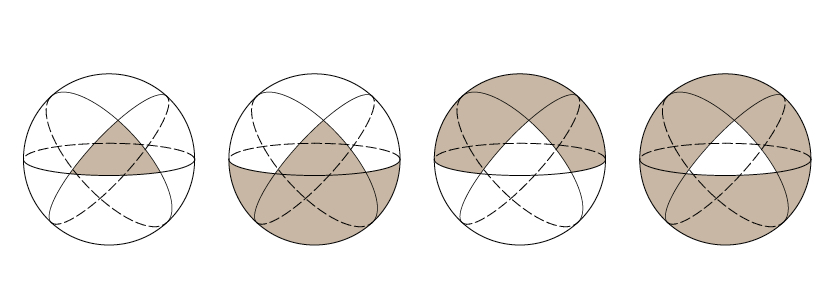
\includegraphics[width=0.9\textwidth]{kugel/Dreieckarten.jpg}
    \captionof{figure}{Dreieckarten auf einer Kugeloberfläche}
\end{center}

Der Begriff Sphärisches Dreieck oder Kugeldreieck ist ein sehr weitläufiger Begriff. 
Dabei können wir den Begriff in drei für uns wesentliche Dreiecke unterteilen:

\begin{itemize}
\item Kugelzweieck
\item Nicht Eulersche’Dreiecke
\item Eulersche’Dreiecke
\end{itemize}

\subsection{Kugelzweieck}

Zwei Grosskreise auf der Kugeloberfläche, zerlegen diese in vier gleiche Kugelzweiecke. 
Jedes dieser Dreieckseiten hat die Länge
$180^{\circ}$ oder $\pi$
Der Flächeninhalt wird dabei nur durch den Winkel $\alpha$ zwischen den beiden Grosskreisen bestimmt.

\begin{center}
        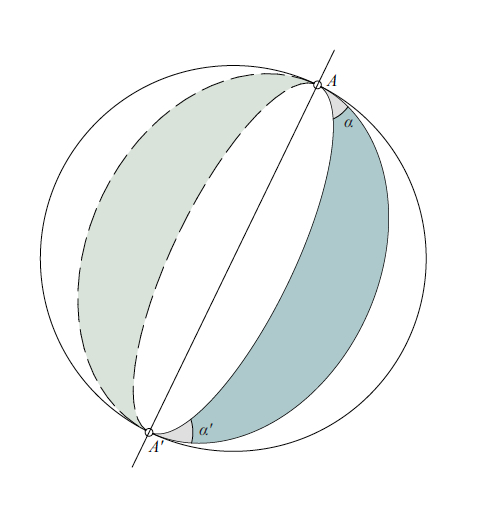
\includegraphics[width=0.3\textwidth]{kugel/Zweieck.jpg}
    \captionof{figure}{Bildung von Zweiecken durch Grosskreise}
\end{center}

Dabei ist der Flächeninhalt der ganzen Kugel:

\begin{align*}
A_{ Kugel } &= 4 \pi r^{2}
\end{align*}


Um den Flächeninhalt des betrachteten Zweieckes zu bekommen, 
müssen wir das ganze noch mit dem Kugelsegment mit dem Winkel $\alpha$ multiplizieren.

\begin{align*}
A_{ Zweieck } &= 4 \pi r^{2} \cdot \frac{ \alpha }{ 2 \pi }
\end{align*}


\subsection{Nicht Eulersche’ Dreiecke}

BLABLA

\subsection{Eulersche’ Dreiecke}

Legt man drei Grosskreise auf eine Kugeloberfläche, bilden sich dabei acht Dreiecke. 
Ein solches Dreieck heisst Eulersches’Dreieck\footnote{%
Leonard Euler (1707-1783), berühmter Schweizer Mathematiker und Physiker. 
Nicht Eulersche’Dreiecke erhält man, indem man das Äussere des Dreieckes ABC betrachtet.} 
Diese Dreiecke werden weder durch die Verlängerung ihrer Seiten durchschnitten, 
noch haben sie Dreiecksseiten welche grösser als $180^{\circ}$ sind.

\begin{center}
        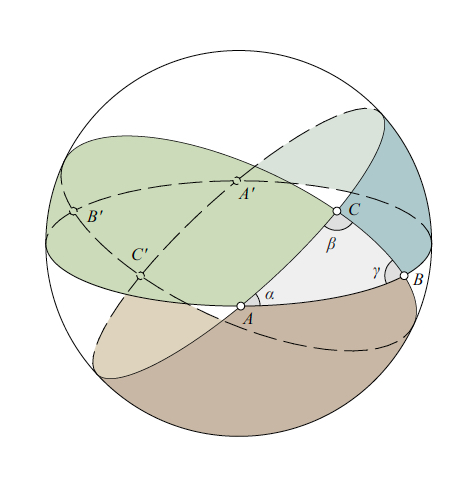
\includegraphics[width=0.4\textwidth]{kugel/Zweiecke.jpg}
    \captionof{figure}{Drei Grosskreise bilden ein sphärisches Dreieck}
\end{center}

In den nachstehenden Erklärungen und Herleitungen, sprechen wir ausschliesslich von Eulerschen’Dreiecken, da die umgeformten Winkelsätze der ebenen Trigonometrie nur auf diese Art von Kugeldreiecken angewendet werden kann.

$A_{ \overline{ ABC }}$ ist die Fläche des Dreieckes auf der Kugeloberfläche
In der ebenen Trigonometrie liegt die Winkelsumme eines Dreiecks bei
$180^{\circ}$.

Anders aber in der sphärischen Trigonometrie. Obschon sie einige Gemeinsamkeiten zur ebenen Trigonometrie aufweist, kann man nicht alles übernehmen.
So auch nicht wie Winkelsumme in einem sphärischen Dreieck.
Diese liegt bei:

\[
\begin{aligned}
\pi
&-
3\pi
&
&\text{\bigg \vert}
&
180^{\circ}
&-
540^{\circ}
\end{aligned}
\]

daraus lässt sich ableiten, das ein einzelner Winkel nicht grösser als $\pi$ oder $180^{\circ}$ sein darf. Ansonsten ist es kein Eulersches’Dreieck und wir dürfen die sphärische Trigonometrie nicht anwenden.\\
Wichtig anzumerken ist, dass die Seiten immer in Radiant beschrieben werden und nicht im Längenmass Meter wie wir es uns gewohnt sind. 
Bei den Dreiecksseiten handelt es sich um Kreisbögen und keine Strecken.

\section{Dreiecksfläche}

\begin{align*}
\text{Zweieck A}
&=
\overline{ABC} + \overline{A'BC} = 2 \alpha r^{ 2 } = A_{ \alpha }\\
\text{Zweieck B}
&=
\overline{ABC} + \overline{AB'C} = 2 \beta r^{ 2 } = A_{ \beta }\\
\text{Zweieck C}
&=
\overline{ABC} + \overline{ABC'} = 2 \gamma r^{ 2 } = A_{ \gamma }
\end{align*}

\begin{align*}
A_{ \alpha } + A_{ \beta } + A_{ \gamma } &= \frac{ 4\pi r^{ 2 } }{ 2 } + 2A_{ \overline{ ABC }} \\
2\alpha r^{ 2 } + 2\beta r^{ 2 } + 2\gamma r^{ 2 } &= \frac{ 4\pi r^{ 2 } }{ 2 } + 2A_{ \overline{ ABC }} \parallel:2\\
\alpha r^{ 2 } + \beta r^{ 2 } + \gamma r^{ 2 } &= \pi r^{ 2 } + A_{ \overline{ ABC }} \parallel-\pi r^{ 2 }\\
r^{ 2 }\left(\alpha + \beta + \gamma - \pi\right) &= A_{ \overline{ ABC }}
\end{align*}




\section{Sphärischer Exzess}
Die Winkelsumme sphärischer Dreiecke ist immer \textgreater \,  $\pi$.

\begin{align*}
\pi < \alpha + \beta + \gamma
\end{align*}

Der sphärische Exzess gibt dabei an, wie stark die Winkelsumme von $\pi$ abweicht.

\begin{align*}
\pi + \epsilon &= \alpha + \beta + \gamma \\
\epsilon &= \alpha + \beta + \gamma - \pi
\end{align*}

Würde der sphärische Exzess in der ebenen Trigonometrie angewendet, wäre dieser = 0. 
Bezieht man das auf die Erde und somit einer Kugel, kann man mit Hilfe eines beliebigen sphärischen Dreieckes und dessen Flächeninhalt auf den Radius der Kugel schliessen.

\subsection{Grenzfall - Satz von Legendre}

\begin{quote} \textit{Ein kleines sphärisches Dreieck kann näherungsweise 
wie ein ebenes Dreieck mit denselben Seiten berechnet 
werden, wenn alle Winkel des ebenen Dreiecks die um 
je ein Drittel des sphärischen Exzesses verminderten 
Winkel des sphärischen Dreiecks nimmt.} \end{quote}
\begin{flushright} - Adrien-Marie Legendre (1752-1833), Paris 1787
\end{flushright}x

Diese Aussage zeigt den Zusammenhang zwischen der 
Trigonometrie in der Ebene sowie in auf der Kugel
auf. Im speziellen bei sehr kleinen sphärischen 
Dreiecken ist die Winkelsumme nur unwesentlich 
grösser als $180^{\circ}$. Des Weiteren kann gesagt werden,
dass der sphärische Exzess gleichmässig auf alle
Winkel aufgeteilt wird.
Wichtig anzumerken ist, dass der Satz von Legendre 
für grosse, aber endliche Radien $r$ gilt.

%[SKIZZE GROSSER RADIUS/KLEINE KRÜMMUNG, KLEINER RADIUS/GROSSE KRÜMMUNG!!!!]
%


\section{Sphärisch Analoge Winkelfunktionen}

\subsection{Sphärischer Sinussatz}

Wir stellen die allgemeinen Sinussätze der Winkel $\alpha$ und $\gamma$ auf:


\[
\begin{aligned}
&{sin(\gamma)} = \frac{h}{a}
&
&\text{\bigg \vert}
&
&{sin(\alpha)} = \frac{h}{c}
&
\end{aligned}
\]

Daraus folgt:
\begin{align*}
h &= sin(\gamma)\cdot a \\
h &= sin(\alpha)\cdot c
\end{align*} 

Durch Gleichsetzung erhält man:
\begin{align*}
h &= h \\
sin(\gamma)\cdot a &= sin(\alpha)\cdot c
\end{align*} 

Durch umstellen erhalten wir den Sinussatz für a und c:
\begin{align*}
sin(\gamma)\cdot a &= sin(\alpha)\cdot c \\
\frac{sin(\gamma)}{c} &= \frac{sin(\alpha)}{a} 
\end{align*} 



\begin{align*}
\frac{sin(\alpha)}{sin(a)} = \frac{sin(\beta)}{sin(b)} = \frac{sin(\gamma)}{sin(c)}
\end{align*} 


\subsection{Winkelkosinussatz}

%[SKIZZE WINKELKOSINUS]

\[
\begin{aligned}
&\overline{C'A'} &= d\cdot {tan(b)}
&
&
&
&
&
&\overline{C'B'} &= d\cdot {tan(a)}
\end{aligned}
\]

\[
\begin{aligned}
&\overline{MA'} &= \frac{ d }{cos(b)}
&
&
&
&
&
&\overline{MB'} &= \frac{ d }{cos(a)}
\end{aligned}
\]

Der allgemeine Kosinussatz beschreibt sich wie folgt:

\begin{align*}
c^{ 2 } &= a^{ 2 } + b^{ 2 } - 2ab \cdot cos(\gamma)
\end{align*}

\begin{align*}
\triangle \overline{A'B'C' }
\overline{ A'B' }^{ 2 } &= \overline{ C'B' }^{ 2 } + \overline{ C'A' }^{ 2 } - 2 \cdot \overline{ C'B' } \cdot \overline{ C'A' } \cdot cos(\gamma)
\end{align*}



\begin{align*}
\overline{A'B'}^{ 2 } &= (d\cdot tan(a))^{ 2 } + (d\cdot tan(b))^{ 2 } - 2 \cdot (d\cdot tan(a) \cdot (d\cdot tan(b) \cdot cos(\gamma)\\
\overline{A'B'}^{ 2 } &= d^{ 2 } \cdot \left(\left(tan^{ 2 }(a) + tan^{ 2 }(b)\right) - 2\cdot tan(a) \cdot tan(b) \cdot cos(\gamma)\right)
\end{align*}

\begin{align*}
\triangle \overline{ MA'B' }
\overline{ A'B' }^{ 2 } &= \overline{ MB' }^{ 2 } + \overline{ MA' }^{ 2 } - 2\cdot \overline{ MB'} \cdot \overline{ MA' } \cdot cos(c)
\end{align*}


\begin{align*}
\overline{ A'B'}^{ 2 } &= \left(\frac{ d }{ cos(a) }  \right)^{ 2 } + \left(\frac{ d }{ cos(b)}  \right)^{ 2 } - 2 \cdot \frac{ d }{ cos(a)} \cdot \frac{ d }{ cos(b)} \cdot cos(c) \\
\overline{ A'B' }^{ 2 } &= d^{ 2 } \cdot \left(\left(\frac{ 1 }{ cos(a) }  \right)^{ 2 } + \left(\frac{ 1 }{ cos(b) }  \right)^{ 2 } - 2 \cdot \frac{ 1 }{ cos(a)} \cdot \frac{ 1 }{ cos(b)} \cdot cos(c)\right)\\
\overline{ A'B' }^{ 2 } &= d^{ 2 } \cdot \left(\left(tan^{ 2 }(a) + 1\right) + \left(tan^{ 2 }(b) + 1\right) - \left(2 \cdot \frac{cos(c)}{cos(a) \cdot cos(b)}\right)\right)
\end{align*}



\begin{align*}
\overline{ A'B'}^{ 2 } &= d^{ 2 } \cdot \left(\left(tan^{ 2 }(a) + tan^{ 2 }(b)\right) - 2 \cdot tan(a) \cdot tan(b) \cdot cos(\gamma)\right) \\
\overline{ A'B'}^{ 2 } &= d^{ 2 } \cdot \left(\left(tan^{ 2 }(a) + 1\right) + \left(tan^{ 2 }(b) + 1\right) - \left(2 \cdot \frac{cos(c)}{cos(a) \cdot cos(b)}\right)\right)
\end{align*}

Die anderen Gleichungen des Satzes, erfolgen aus Symmetriegründen.

\subsection{Seitenkosinussatz}
Durch zyklische Vertauschung des Winkelkosinus erhalten wir den Seitenkosinussatz:

\begin{align*}
{cos(a)} &= {cos(b)} \cdot {cos(c)} + {sin(b)} \cdot {sin(c)} \cdot {sin(\alpha)}\\
{cos(b)} &= {cos(a)} \cdot {cos(c)} + {sin(a)} \cdot {sin(c)} \cdot {sin(\beta)}\\
{cos(c)} &= {cos(a)} \cdot {cos(b)} + {sin(a)} \cdot {sin(b)} \cdot {sin(\gamma)}\\
\end{align*}

\section{Navigation auf See}
Das besondere an Seekarten ist die Inhaltliche Ausrichtung. Anders wie Landkarten muss sie Informationen enthalten welche für den Kapitän und seine Besatzung von grosser Bedeutung sind. Vor allem in Küstennähe ist das navigieren eines Schiffes besonders gefährlich. So enthalten Seekarten etwas über Wassertiefen, Bodenbeschaffenheiten, Gezeiten, Küstenlinien, Landzungen und Windrichtungen.
Der Hauptunterschied dabei ist, das auf der Landkarte feste Positionen definiert und aufgezeigt werden, das einzige was sich verändert ist der Reisende selbst. Bei der Seekarte ist das anders, es werden veränderliche Einwirkungen der Natur festgehalten.

Dieser kleine Unterschied zeigt die Notwendigkeit auf, die Position und den Kurs seines Schiffes auf See immer ermitteln zu können.


\section{Geographische Koordinaten}

Nachdem klar war, das die Erde eine Kugel ist, wurde diese in ein Gradnetz aufgeteilt. Dabei wurden die Angaben für eine exakte Ortsbestimmung klar definiert und die bis heute gültigen Koordinaten bestimmt.
Dabei muss man sich nochmals in Erinnerung rufen, dass sich die Erde in 24h einmal um ihre eigene Achse dreht. Nach $360 ^{\circ}$ 
und somit einer vollen Umdrehung, steht sie wieder in ihrer Ursprungsposition und ein neuer Tag beginnt.

Die Koordinaten setzen sich aus folgenden Komponenten zusammen:

\[
\begin{aligned}
&\text{Grad } (^{\circ})
&
&\text{\bigg \vert}
&
&\text{Bogenminuten } (`)
&
&\text{\bigg \vert}
&
&\text{Bogensekunden } (``)
\end{aligned}
\]

Die Erdoberfläche wurde in je 360 Breiten- und Längengrade eingeteilt. Die Breitengrade haben zueinander einen Abstand von 111.31 km, dies entspricht auch dem Abstand der Längengrade am Äquator mit Zunehmender Nähe zu den Polen, nimmt dieser Abstand ab.

\[
\begin{aligned}
&1^{\circ}
&
&\text{\bigg \vert}
&
&4 \text{ Minuten}
&
&\text{\bigg \vert}
&
&111.31\text{ km}
\end{aligned}
\]

Berechnet man nun die Erdumdrehung von 360°, erhält man genau den Erdumfang am Äquator: \begin{align*} 40’074 \text{ km.}\end{align*}

Dabei geben die Bogenminuten und -sekunden dem Standort die gewünschte Exaktheit. Mit den vollständigen Koordinaten lässt sich der Standort auf einer Landkarte exakt bestimmen und einzeichnen.

\subsection{Zeitzonen der Erde}
Wenn man nun die verschiedenen Zeitzonen der Erde betrachtet, macht die Verschiebung von jeweils einer Stunde durchaus Sinn, es lässt sich auf die Längengrade schliessen.
Zwischen den verschiedenen Zeitzonen liegen 15 Längengrade:

\begin{align*}
\text{15 Längengrade à 4 Minuten = 60 Minuten Zeitverschiebung = ca. 1665 km}
\end{align*}

Dabei ist die Zeitzone in welcher Mitte sich der Greenwich Meredian befindet die \textit{Greenwich Mean Time (GMT)} welche bis 1928 als Weltzeit galt. Im Jahr 1972 wurde diese umbenannt in die \textit{Coordinated Universal Time (UTC)} und wir von da an als Weltzeit $\pm$ 0.00 verwendet.


\section{Der Breitengrad}
Die Breitengrade bilden die bereits genannten Kleinkreise auf der Kugeloberfläche. Sie verlaufen in einem Abstand von genau 111 km parallel zum Äquator. Dabei stellt  dieser genau die Mitte zwischen Nord- und Südpol dar und teilt die Erdkugel in zwei gleiche Hälften. Somit wird von nördlicher und südlicher Breite gesprochen, je nach dem auf welcher Halbkugel man sich befindet.

%[SKIZZE DER GEOGRAFISCHEN BREITE ERDKUGEL]

\subsection{Geografische Breite $\phi$}
\begin{definition}
Die geografische Breite eines Standortes ist nichts anderes, als der Winkel am Erdmittelpunkt zwischen der Ebene des Äquators und der Geraden zum Standpunkt auf der Erdoberfläche.
\end{definition}

%[SKIZZE DER GEOGRAFISCHEN BREITE MIT WINKEL]

\subsection{Navigation mit den Breitengraden}
Da der Breitengrad bereits sehr früh ziemlich präzise bestimmt werden könnte, nutzten bereits die Seefahrer um Christoph Kolumbus den Breitengrad zur Navigation ihrer Flotten.
Den dieser lässt sich ziemlich einfach aus dem höchsten Sonnenstand oder einem Fixstern bestimmen. Dabei wird mit einem Jakobsstab\footnote{%
Der Jakobsstab ist ein früheres astronomisches Instrument zur Winkelmessung und wurde vor allem in der Seefahrt verwendet. Er ist in der Nautik der Vorläufer des Sextanten.} (später Sextant\footnote{%
Der Sextant ist ein nautisches Messinstrument zur Winkelmessung von Horizont und Fixstern (Gestirn)}) der Winkel zwischen dem Horizont und dem Fixstern gemessen. Der Winkel welchen man erhält, zieht man von 90° ab und erhält somit die geografische Breite. \\

%[SKIZZE ERMITTLUNG DES BREITENGRADES]

Wenn man sich auf der Nordhalbkugel befindet, ist der Polarstern ein sehr guter Fixstern. Befindet sich ein Schiff nun sehr nahe am Nordpol, steht dieser nahezu senkrecht am Himmelszelt bei $90^{\circ}$. Würde es aber nahe dem Äquator stehen, erscheint dieser am Horizont bei $0^{\circ}$.

\subsection{Korrekturbeiwert}

\section{Der Längengrad}
Die Längengrade bilden die bereits genannten Grosskreise auf der Kugeloberfläche.
Sie schneiden den Äquator im rechten Winkel, haben dort einen Abstand von 111 km zueinander und verbinden die Pole. Anders wie bei der geografischen Breite, ist in der Natur kein Längengrad gegeben welcher den Nullpunkt darstellt.

%[SKIZZE DER GEOGRAFISCHEN LÄNGE ERDKUGEL]

\subsection{Geografische Länge $\lambda$}
\begin{definition}
Die geografische Länge ist der Winkel an der Erdachse zum Nullmeridian.
\end{definition}

\subsection{Navigation mit den Längengraden}
Die geografische Länge lässt sich nicht so einfach bestimmen wie deren Breite. Für die Berechnung auf See benötigt man eine Referenzzeit eines Ortes mit bekannter Länge.
In der Zeit der Entdecker gab es noch keine mechanischen Uhren. Die Sonnenuhr war zudem ungeeignet, da diese nur die Uhrzeit am Standort mass und nicht die am Referenzort selbst. Die erste Pendeluhr wurde erst Mitte des 17. Jahrhunderts erfunden, was in der Schifffahrt aber auch nicht die Lösung brachte.\\
Pendeluhren auf einem Schiff sind ungeeignet, da das Pendel mit dem Wellengang aus dem Takt gebracht wird und somit die Uhr falsch geht.
Zu ungenau und gegen äussere Erschütterungen zu empfindlich waren später auch die federgetriebenen Uhren und die Unruh. Dazukamen die verschiedenen Klimazonen welche ein Schiff zu durchqueren hatten. Das Metall zog sich viel zu fest zusammen oder dehnte sich aus, was dazu führte das die Uhr unregelmässig lief.

Das sogenannte „Längenproblem“ stellte nicht nur bei der Navigation auf See ein Problem dar, es ergaben sich auch wirtschaftliche Konsequenzen. Die Schiffe mussten bis zur gewünschten geografischen Breite navigieren und segelten dann den Breitengrad entlang. Dabei waren die Schiffe oft Wochenlang unterwegs und segelten die „Breiten ab“ um an die gewünschte Position zu kommen. Dies führte zu erheblichen Zeitverlusten und viel längeren Reisezeiten.


\section{The Board of Longitude - Das Längenproblem}
Das Längenproblem beschäftigte alle grossen Seefahrernationen Europas. Wenn man bedenkt das sich Werte in einer  Höhe von halben britischen Staatshaushalten auf verloren gegangenen Schiffen befanden, erkennt man die Dringlichkeit für eine zuverlässige und genaue Navigation auf See.


\begin{itemize}
\item £ 20’000 - Abweichung von max. einem halben Grad
\item £ 15’000 - Abweichung von zwei Drittel Grad
\item £ 10’000 - Abweichung von max. $1 ^{\circ}$
\end{itemize}

\subsection{John Harrison}


\subsection{Tobias Mayer}



Uhren mit einer Abweichung von einer Minute Abweichung pro Tag (





\section{Nautische Dreieck}


$\Rightarrow$





\section{Die Vermessung der Welt}
Wir schreiben das Jahr 1818 und kehren in die Zeit des Mathematikers Carl Friedrich Gauss zurück. Neben dem liebevoll genannten „kleinen Gauss“ und anderen herausragenden Mathematischen Leistungen, beschäftigte er in den Folgejahren mit der Vermessung des Königreichs Hannovers und verfasste auf 61 Blättern das Kartenwerk \textit{Gauss’sche Landesaufnahme der 1815 durch Hannover erworbenen Gebiete}.






AUFGABE

Hubble Teleskop 
24. April 1990






\printbibliography[heading=subbibliography]
\end{refsection}




%\chapter{Geometrie auf der Kugeloberfläche\label{chapter:kugel}}
\lhead{Geometrie auf der Kugeloberfläche}
\begin{refsection}
\chapterauthor{Melina Staub und Fabian Schmid}

\section{Einleitung}

Schon seit jeher fasziniert den Menschen die Fahrt zur See. Nicht grundlos ist die Seefahrt eine der wichtigsten und ältesten Tätigkeiten der Menschheit. Der innerliche Drang neue Weltmeere und unbekannte Gebiete zu entdecken, die Fahrt zur See zu erleichtern und erträglicher zu machen, trieben die Menschen an, die Schiffe dieser Welt immer weiter zu entwickeln.

Die Idee der Kugelform der Erde ist älter als man zu denken vermag. Bereits der Schüler des antiken griechischen Philosophen Platon - Aristoteles schrieb in seiner Schrift \textit{Über den Himmel} aus dem 4. Jahrhundert v. Chr. etliche Gründe welche für die Gestallt der Erde als Kugel sprechen:

\begin{itemize}
      \item Sämtliche schweren Körper streben zum Mittelpunkt des Alls. Da sie dies von allen Seiten her gleichmäßig tun und die Erde im Mittelpunkt des Alls steht, muss sie eine kugelrunde Gestalt annehmen. 
\item Bei von der Küste wegfahrende Schiffen wird der Rumpf vor den Segeln der Sicht verborgen. 
\item In südlichen Ländern erscheinen südliche Sternbilder höher über dem Horizont.
\item Der Erdschatten bei einer Mondfinsternis ist stets rund.
\end{itemize}

Jedoch war um 1492 - der Zeit der Entdeckung Amerikas durch Christoph Kolumbus, die Idee der Erde in Kugelform noch sehr umstritten. Er erkannte anhand den Theorien und Erkenntnissen der alten Griechen, vor allem Aristoteles, das die Erde eine Kugel sein muss. \\
Doch mit seinem Vorschlag einen Seeweg über den Atlantik nach Indien zu finden und nicht wie üblich um Afrika zu segeln, stiess er beim beim portugiesischen König auf taube Ohren. Sein Plan Indien über eine Route nach Westen zu erreichen, widersprach dem gesunden Menschenverstand. Wäre die Erde wirklich eine Kugel und man befände sich auf der unteren Erdhalbkugel, würde man herunterfallen.\\
Doch auch der damals übliche Glaube an die Erde in Scheibenform brachte so einige Risiken mit sich. Was würde passieren, wenn die Flotte das Ende der Scheibe erreicht hatte? Würden sie über den Erdrand hinweggleiten und in den Abgrund stürzen?\\
Erst nach viel Überzeugungsarbeit durch Kolumbus, setzte er sich am Spanischen Hof durch und segelte über die Westliche Route über den Atlantik und entdeckte schlussendlich Amerika.

Der praktische und greifbare Beweis das die Erde eine Kugel ist, lieferte rund 30 Jahre später der Portugiese Fernando Magellan. Mit seiner Weltumsegelung und seiner Ankunft in den Philippinen, bewies er definitiv das die Erde eine Kugel ist.\\

Nun wollen wir uns die Frage stellen, wie die alten Seefahrer ohne GPS und jeglichen modernen Navigationssystemen auf hoher See wussten wo sie sich befinden und was haben die Sterne mit alldem zu tun? Reisen Sie mit uns zurück in eine Zeit mit Sextant, Kompass und Sternkarten. In die Zeit der Seefahrer und Entdecker.


\section{Geometrie auf der Ebene und der Kugel}

Euklid von Alexandria beschrieb die Grundbegriffe der ebenen Geometrie mittels Punkt, Geraden, Ebene, Winkel und Dreieck. Diese Dreiecke lassen sich mithilfe der ebenen Trigonometrie beschreiben. Dabei gelten die uns bekannten trigonometrischen Winkelfunktionen:\\

\text{Sinussatz:}
\begin{align*}
\frac{ a }{ sin(\alpha) } &= \frac{ b }{sin(\beta)} = \frac{ c }{ sin(\gamma) } = \frac{abc}{2A} = 2r\\
\end{align*}

\text{Cosinussatz:}
\begin{align*}
c^{ 2 } &= a^{ 2 } + b^{ 2 } - 2ab\cdot cos(\gamma)\\
b^{ 2 } &= a^{ 2 } + c^{ 2 } - 2ab\cdot cos(\beta)\\
a^{ 2 } &= b^{ 2 } + c^{ 2 } - 2ab\cdot cos(\alpha)
\end{align*}

Um Dreiecke auf der Kugeloberfläche zu berechnen, benötigt man die sphärische Trigonometrie. Die oben beschriebenen Sätze lassen sich auf der Kugel nicht anwenden, sie werden aber als Grundlage zur Herleitung der Sätze für das Kugeldreieck benötigt.

Die nachfolgenden Seiten thematisieren die Geometrie auf der Kugeloberfläche und wie sie in der Navigation eingesetzt werden kann.


\section{Gross- und Kleinkreise}

Eine Kugeloberfläche lässt sich in zwei verschiedene Kreisarten einteilen -  Gross- und Kleinkreise. 
Wir betrachten als erstes die Grosskreise:

\begin{definition}
Ein Großkreis ist ein größtmöglicher Kreis auf einer Kugeloberfläche. Sein Mittelpunkt fällt immer mit dem Mittelpunkt der Kugel zusammen und ein Schnitt auf dem Großkreis teilt die Kugel in jedem Fall in zwei („gleich große“) Hälften.
\end{definition}

Es gibt unendlich viele Möglichkeiten, eine Kugel in zwei gleich grosse Stücke zu zerschneiden, 
daher gibt es auch unendlich viele Grosskreise. Wenn wir die Grosskreise auf einer Kugel mit diesen auf der Erde beschreiben, sprechen wir von den Längengraden aber auch der Äquator beschreibt einen Grosskreis.
Ein Elementarer Bestandteil bilden die Grosskreise in der sphärischen Trigonometrie. Mithilfe der Schnittpunkte verschiedener Grosskreise, lässt sich ein Sphärisches Dreieck bilden auf welchem sich die sphärische Trigonometrie anwenden lässt.

[GRAFIK GROSSKREISE]

\begin{definition}
Unter Kleinkreis versteht man jene Kreise auf einer Kugeloberfläche, deren Ebenen nicht den Kugelmittelpunkt enthalten.
\end{definition}

Die Kleinkreise eignen sich im Gegensatz zu den Grosskreisen \textit{nicht} für die sphärische Trigonometrie. 
Sie werden lediglich zur Bestimmung der Messgrössen, Winkelabstände oder des Höhenwinkels eines Gestirns verwendet. 

Wenn wir die Kleinkreise auf die Erdoberfläche projizieren betrachten wir die Breitengrade.

[GRAFIK KLEINKREISE]


\section{Sphärische Dreiecke / Kugeldreieck}

\begin{center}
        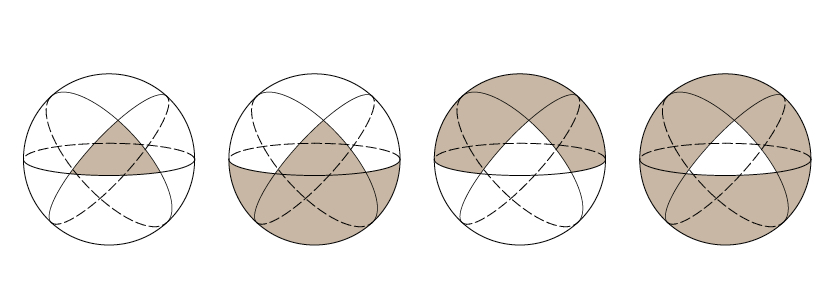
\includegraphics[width=0.9\textwidth]{kugel/Dreieckarten.jpg}
    \captionof{figure}{Dreieckarten auf einer Kugeloberfläche}
\end{center}

Der Begriff Sphärisches Dreieck oder Kugeldreieck ist ein sehr weitläufiger Begriff. 
Dabei können wir den Begriff in drei für uns wesentliche Dreiecke unterteilen:

\begin{itemize}
\item Kugelzweieck
\item Nicht Eulersche’Dreiecke
\item Eulersche’Dreiecke
\end{itemize}

\subsection{Kugelzweieck}

Zwei Grosskreise auf der Kugeloberfläche, zerlegen diese in vier gleiche Kugelzweiecke. 
Jedes dieser Dreieckseiten hat die Länge
$180^{\circ}$ oder $\pi$
Der Flächeninhalt wird dabei nur durch den Winkel $\alpha$ zwischen den beiden Grosskreisen bestimmt.

\begin{center}
        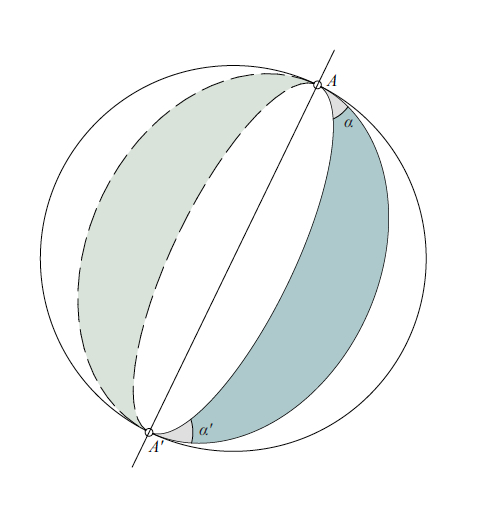
\includegraphics[width=0.3\textwidth]{kugel/Zweieck.jpg}
    \captionof{figure}{Bildung von Zweiecken durch Grosskreise}
\end{center}

Dabei ist der Flächeninhalt der ganzen Kugel:

\begin{align*}
A_{ Kugel } &= 4 \pi r^{2}
\end{align*}


Um den Flächeninhalt des betrachteten Zweieckes zu bekommen, 
müssen wir das ganze noch mit dem Kugelsegment mit dem Winkel $\alpha$ multiplizieren.

\begin{align*}
A_{ Zweieck } &= 4 \pi r^{2} \cdot \frac{ \alpha }{ 2 \pi }
\end{align*}


\subsection{Nicht Eulersche’ Dreiecke}

BLABLA

\subsection{Eulersche’ Dreiecke}

Legt man drei Grosskreise auf eine Kugeloberfläche, bilden sich dabei acht Dreiecke. 
Ein solches Dreieck heisst Eulersches’Dreieck\footnote{%
Leonard Euler (1707-1783), berühmter Schweizer Mathematiker und Physiker. 
Nicht Eulersche’Dreiecke erhält man, indem man das Äussere des Dreieckes ABC betrachtet.} 
Diese Dreiecke werden weder durch die Verlängerung ihrer Seiten durchschnitten, 
noch haben sie Dreiecksseiten welche grösser als $180^{\circ}$ sind.

\begin{center}
        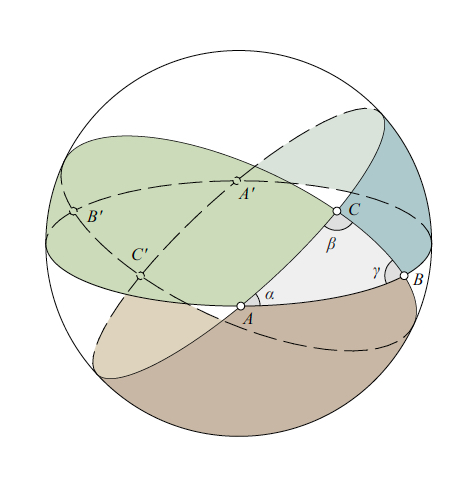
\includegraphics[width=0.4\textwidth]{kugel/Zweiecke.jpg}
    \captionof{figure}{Drei Grosskreise bilden ein sphärisches Dreieck}
\end{center}

In den nachstehenden Erklärungen und Herleitungen, sprechen wir ausschliesslich von Eulerschen’Dreiecken, da die umgeformten Winkelsätze der ebenen Trigonometrie nur auf diese Art von Kugeldreiecken angewendet werden kann.

$A_{ \overline{ ABC }}$ ist die Fläche des Dreieckes auf der Kugeloberfläche
In der ebenen Trigonometrie liegt die Winkelsumme eines Dreiecks bei
$180^{\circ}$.

Anders aber in der sphärischen Trigonometrie. Obschon sie einige Gemeinsamkeiten zur ebenen Trigonometrie aufweist, kann man nicht alles übernehmen.
So auch nicht wie Winkelsumme in einem sphärischen Dreieck.
Diese liegt bei:

\[
\begin{aligned}
\pi
&-
3\pi
&
&\text{\bigg \vert}
&
180^{\circ}
&-
540^{\circ}
\end{aligned}
\]

daraus lässt sich ableiten, das ein einzelner Winkel nicht grösser als $\pi$ oder $180^{\circ}$ sein darf. Ansonsten ist es kein Eulersches’Dreieck und wir dürfen die sphärische Trigonometrie nicht anwenden.\\
Wichtig anzumerken ist, dass die Seiten immer in Radiant beschrieben werden und nicht im Längenmass Meter wie wir es uns gewohnt sind. 
Bei den Dreiecksseiten handelt es sich um Kreisbögen und keine Strecken.

\section{Dreiecksfläche}

\begin{align*}
\text{Zweieck A}
&=
\overline{ABC} + \overline{A'BC} = 2 \alpha r^{ 2 } = A_{ \alpha }\\
\text{Zweieck B}
&=
\overline{ABC} + \overline{AB'C} = 2 \beta r^{ 2 } = A_{ \beta }\\
\text{Zweieck C}
&=
\overline{ABC} + \overline{ABC'} = 2 \gamma r^{ 2 } = A_{ \gamma }
\end{align*}

\begin{align*}
A_{ \alpha } + A_{ \beta } + A_{ \gamma } &= \frac{ 4\pi r^{ 2 } }{ 2 } + 2A_{ \overline{ ABC }} \\
2\alpha r^{ 2 } + 2\beta r^{ 2 } + 2\gamma r^{ 2 } &= \frac{ 4\pi r^{ 2 } }{ 2 } + 2A_{ \overline{ ABC }} \parallel:2\\
\alpha r^{ 2 } + \beta r^{ 2 } + \gamma r^{ 2 } &= \pi r^{ 2 } + A_{ \overline{ ABC }} \parallel-\pi r^{ 2 }\\
r^{ 2 }\left(\alpha + \beta + \gamma - \pi\right) &= A_{ \overline{ ABC }}
\end{align*}




\section{Sphärischer Exzess}
Die Winkelsumme sphärischer Dreiecke ist immer \textgreater \,  $\pi$.

\begin{align*}
\pi < \alpha + \beta + \gamma
\end{align*}

Der sphärische Exzess gibt dabei an, wie stark die Winkelsumme von $\pi$ abweicht.

\begin{align*}
\pi + \epsilon &= \alpha + \beta + \gamma \\
\epsilon &= \alpha + \beta + \gamma - \pi
\end{align*}

Würde der sphärische Exzess in der ebenen Trigonometrie angewendet, wäre dieser = 0. 
Bezieht man das auf die Erde und somit einer Kugel, kann man mit Hilfe eines beliebigen sphärischen Dreieckes und dessen Flächeninhalt auf den Radius der Kugel schliessen.

\subsection{Grenzfall - Satz von Legendre}

\begin{quote} \textit{Ein kleines sphärisches Dreieck kann näherungsweise 
wie ein ebenes Dreieck mit denselben Seiten berechnet 
werden, wenn alle Winkel des ebenen Dreiecks die um 
je ein Drittel des sphärischen Exzesses verminderten 
Winkel des sphärischen Dreiecks nimmt.} \end{quote}
\begin{flushright} - Adrien-Marie Legendre (1752-1833), Paris 1787
\end{flushright}x

Diese Aussage zeigt den Zusammenhang zwischen der 
Trigonometrie in der Ebene sowie in auf der Kugel
auf. Im speziellen bei sehr kleinen sphärischen 
Dreiecken ist die Winkelsumme nur unwesentlich 
grösser als $180^{\circ}$. Des Weiteren kann gesagt werden,
dass der sphärische Exzess gleichmässig auf alle
Winkel aufgeteilt wird.
Wichtig anzumerken ist, dass der Satz von Legendre 
für grosse, aber endliche Radien $r$ gilt.

%[SKIZZE GROSSER RADIUS/KLEINE KRÜMMUNG, KLEINER RADIUS/GROSSE KRÜMMUNG!!!!]
%


\section{Sphärisch Analoge Winkelfunktionen}

\subsection{Sphärischer Sinussatz}

Wir stellen die allgemeinen Sinussätze der Winkel $\alpha$ und $\gamma$ auf:


\[
\begin{aligned}
&{sin(\gamma)} = \frac{h}{a}
&
&\text{\bigg \vert}
&
&{sin(\alpha)} = \frac{h}{c}
&
\end{aligned}
\]

Daraus folgt:
\begin{align*}
h &= sin(\gamma)\cdot a \\
h &= sin(\alpha)\cdot c
\end{align*} 

Durch Gleichsetzung erhält man:
\begin{align*}
h &= h \\
sin(\gamma)\cdot a &= sin(\alpha)\cdot c
\end{align*} 

Durch umstellen erhalten wir den Sinussatz für a und c:
\begin{align*}
sin(\gamma)\cdot a &= sin(\alpha)\cdot c \\
\frac{sin(\gamma)}{c} &= \frac{sin(\alpha)}{a} 
\end{align*} 



\begin{align*}
\frac{sin(\alpha)}{sin(a)} = \frac{sin(\beta)}{sin(b)} = \frac{sin(\gamma)}{sin(c)}
\end{align*} 


\subsection{Winkelkosinussatz}

%[SKIZZE WINKELKOSINUS]

\[
\begin{aligned}
&\overline{C'A'} &= d\cdot {tan(b)}
&
&
&
&
&
&\overline{C'B'} &= d\cdot {tan(a)}
\end{aligned}
\]

\[
\begin{aligned}
&\overline{MA'} &= \frac{ d }{cos(b)}
&
&
&
&
&
&\overline{MB'} &= \frac{ d }{cos(a)}
\end{aligned}
\]

Der allgemeine Kosinussatz beschreibt sich wie folgt:

\begin{align*}
c^{ 2 } &= a^{ 2 } + b^{ 2 } - 2ab \cdot cos(\gamma)
\end{align*}

\begin{align*}
\triangle \overline{A'B'C' }
\overline{ A'B' }^{ 2 } &= \overline{ C'B' }^{ 2 } + \overline{ C'A' }^{ 2 } - 2 \cdot \overline{ C'B' } \cdot \overline{ C'A' } \cdot cos(\gamma)
\end{align*}



\begin{align*}
\overline{A'B'}^{ 2 } &= (d\cdot tan(a))^{ 2 } + (d\cdot tan(b))^{ 2 } - 2 \cdot (d\cdot tan(a) \cdot (d\cdot tan(b) \cdot cos(\gamma)\\
\overline{A'B'}^{ 2 } &= d^{ 2 } \cdot \left(\left(tan^{ 2 }(a) + tan^{ 2 }(b)\right) - 2\cdot tan(a) \cdot tan(b) \cdot cos(\gamma)\right)
\end{align*}

\begin{align*}
\triangle \overline{ MA'B' }
\overline{ A'B' }^{ 2 } &= \overline{ MB' }^{ 2 } + \overline{ MA' }^{ 2 } - 2\cdot \overline{ MB'} \cdot \overline{ MA' } \cdot cos(c)
\end{align*}


\begin{align*}
\overline{ A'B'}^{ 2 } &= \left(\frac{ d }{ cos(a) }  \right)^{ 2 } + \left(\frac{ d }{ cos(b)}  \right)^{ 2 } - 2 \cdot \frac{ d }{ cos(a)} \cdot \frac{ d }{ cos(b)} \cdot cos(c) \\
\overline{ A'B' }^{ 2 } &= d^{ 2 } \cdot \left(\left(\frac{ 1 }{ cos(a) }  \right)^{ 2 } + \left(\frac{ 1 }{ cos(b) }  \right)^{ 2 } - 2 \cdot \frac{ 1 }{ cos(a)} \cdot \frac{ 1 }{ cos(b)} \cdot cos(c)\right)\\
\overline{ A'B' }^{ 2 } &= d^{ 2 } \cdot \left(\left(tan^{ 2 }(a) + 1\right) + \left(tan^{ 2 }(b) + 1\right) - \left(2 \cdot \frac{cos(c)}{cos(a) \cdot cos(b)}\right)\right)
\end{align*}



\begin{align*}
\overline{ A'B'}^{ 2 } &= d^{ 2 } \cdot \left(\left(tan^{ 2 }(a) + tan^{ 2 }(b)\right) - 2 \cdot tan(a) \cdot tan(b) \cdot cos(\gamma)\right) \\
\overline{ A'B'}^{ 2 } &= d^{ 2 } \cdot \left(\left(tan^{ 2 }(a) + 1\right) + \left(tan^{ 2 }(b) + 1\right) - \left(2 \cdot \frac{cos(c)}{cos(a) \cdot cos(b)}\right)\right)
\end{align*}

Die anderen Gleichungen des Satzes, erfolgen aus Symmetriegründen.

\subsection{Seitenkosinussatz}
Durch zyklische Vertauschung des Winkelkosinus erhalten wir den Seitenkosinussatz:

\begin{align*}
{cos(a)} &= {cos(b)} \cdot {cos(c)} + {sin(b)} \cdot {sin(c)} \cdot {sin(\alpha)}\\
{cos(b)} &= {cos(a)} \cdot {cos(c)} + {sin(a)} \cdot {sin(c)} \cdot {sin(\beta)}\\
{cos(c)} &= {cos(a)} \cdot {cos(b)} + {sin(a)} \cdot {sin(b)} \cdot {sin(\gamma)}\\
\end{align*}

\section{Navigation auf See}
Das besondere an Seekarten ist die Inhaltliche Ausrichtung. Anders wie Landkarten muss sie Informationen enthalten welche für den Kapitän und seine Besatzung von grosser Bedeutung sind. Vor allem in Küstennähe ist das navigieren eines Schiffes besonders gefährlich. So enthalten Seekarten etwas über Wassertiefen, Bodenbeschaffenheiten, Gezeiten, Küstenlinien, Landzungen und Windrichtungen.
Der Hauptunterschied dabei ist, das auf der Landkarte feste Positionen definiert und aufgezeigt werden, das einzige was sich verändert ist der Reisende selbst. Bei der Seekarte ist das anders, es werden veränderliche Einwirkungen der Natur festgehalten.

Dieser kleine Unterschied zeigt die Notwendigkeit auf, die Position und den Kurs seines Schiffes auf See immer ermitteln zu können.


\section{Geographische Koordinaten}

Nachdem klar war, das die Erde eine Kugel ist, wurde diese in ein Gradnetz aufgeteilt. Dabei wurden die Angaben für eine exakte Ortsbestimmung klar definiert und die bis heute gültigen Koordinaten bestimmt.
Dabei muss man sich nochmals in Erinnerung rufen, dass sich die Erde in 24h einmal um ihre eigene Achse dreht. Nach $360 ^{\circ}$ 
und somit einer vollen Umdrehung, steht sie wieder in ihrer Ursprungsposition und ein neuer Tag beginnt.

Die Koordinaten setzen sich aus folgenden Komponenten zusammen:

\[
\begin{aligned}
&\text{Grad } (^{\circ})
&
&\text{\bigg \vert}
&
&\text{Bogenminuten } (`)
&
&\text{\bigg \vert}
&
&\text{Bogensekunden } (``)
\end{aligned}
\]

Die Erdoberfläche wurde in je 360 Breiten- und Längengrade eingeteilt. Die Breitengrade haben zueinander einen Abstand von 111.31 km, dies entspricht auch dem Abstand der Längengrade am Äquator mit Zunehmender Nähe zu den Polen, nimmt dieser Abstand ab.

\[
\begin{aligned}
&1^{\circ}
&
&\text{\bigg \vert}
&
&4 \text{ Minuten}
&
&\text{\bigg \vert}
&
&111.31\text{ km}
\end{aligned}
\]

Berechnet man nun die Erdumdrehung von 360°, erhält man genau den Erdumfang am Äquator: \begin{align*} 40’074 \text{ km.}\end{align*}

Dabei geben die Bogenminuten und -sekunden dem Standort die gewünschte Exaktheit. Mit den vollständigen Koordinaten lässt sich der Standort auf einer Landkarte exakt bestimmen und einzeichnen.

\subsection{Zeitzonen der Erde}
Wenn man nun die verschiedenen Zeitzonen der Erde betrachtet, macht die Verschiebung von jeweils einer Stunde durchaus Sinn, es lässt sich auf die Längengrade schliessen.
Zwischen den verschiedenen Zeitzonen liegen 15 Längengrade:

\begin{align*}
\text{15 Längengrade à 4 Minuten = 60 Minuten Zeitverschiebung = ca. 1665 km}
\end{align*}

Dabei ist die Zeitzone in welcher Mitte sich der Greenwich Meredian befindet die \textit{Greenwich Mean Time (GMT)} welche bis 1928 als Weltzeit galt. Im Jahr 1972 wurde diese umbenannt in die \textit{Coordinated Universal Time (UTC)} und wir von da an als Weltzeit $\pm$ 0.00 verwendet.


\section{Der Breitengrad}
Die Breitengrade bilden die bereits genannten Kleinkreise auf der Kugeloberfläche. Sie verlaufen in einem Abstand von genau 111 km parallel zum Äquator. Dabei stellt  dieser genau die Mitte zwischen Nord- und Südpol dar und teilt die Erdkugel in zwei gleiche Hälften. Somit wird von nördlicher und südlicher Breite gesprochen, je nach dem auf welcher Halbkugel man sich befindet.

%[SKIZZE DER GEOGRAFISCHEN BREITE ERDKUGEL]

\subsection{Geografische Breite $\phi$}
\begin{definition}
Die geografische Breite eines Standortes ist nichts anderes, als der Winkel am Erdmittelpunkt zwischen der Ebene des Äquators und der Geraden zum Standpunkt auf der Erdoberfläche.
\end{definition}

%[SKIZZE DER GEOGRAFISCHEN BREITE MIT WINKEL]

\subsection{Navigation mit den Breitengraden}
Da der Breitengrad bereits sehr früh ziemlich präzise bestimmt werden könnte, nutzten bereits die Seefahrer um Christoph Kolumbus den Breitengrad zur Navigation ihrer Flotten.
Den dieser lässt sich ziemlich einfach aus dem höchsten Sonnenstand oder einem Fixstern bestimmen. Dabei wird mit einem Jakobsstab\footnote{%
Der Jakobsstab ist ein früheres astronomisches Instrument zur Winkelmessung und wurde vor allem in der Seefahrt verwendet. Er ist in der Nautik der Vorläufer des Sextanten.} (später Sextant\footnote{%
Der Sextant ist ein nautisches Messinstrument zur Winkelmessung von Horizont und Fixstern (Gestirn)}) der Winkel zwischen dem Horizont und dem Fixstern gemessen. Der Winkel welchen man erhält, zieht man von 90° ab und erhält somit die geografische Breite. \\

%[SKIZZE ERMITTLUNG DES BREITENGRADES]

Wenn man sich auf der Nordhalbkugel befindet, ist der Polarstern ein sehr guter Fixstern. Befindet sich ein Schiff nun sehr nahe am Nordpol, steht dieser nahezu senkrecht am Himmelszelt bei $90^{\circ}$. Würde es aber nahe dem Äquator stehen, erscheint dieser am Horizont bei $0^{\circ}$.

\subsection{Korrekturbeiwert}

\section{Der Längengrad}
Die Längengrade bilden die bereits genannten Grosskreise auf der Kugeloberfläche.
Sie schneiden den Äquator im rechten Winkel, haben dort einen Abstand von 111 km zueinander und verbinden die Pole. Anders wie bei der geografischen Breite, ist in der Natur kein Längengrad gegeben welcher den Nullpunkt darstellt.

%[SKIZZE DER GEOGRAFISCHEN LÄNGE ERDKUGEL]

\subsection{Geografische Länge $\lambda$}
\begin{definition}
Die geografische Länge ist der Winkel an der Erdachse zum Nullmeridian.
\end{definition}

\subsection{Navigation mit den Längengraden}
Die geografische Länge lässt sich nicht so einfach bestimmen wie deren Breite. Für die Berechnung auf See benötigt man eine Referenzzeit eines Ortes mit bekannter Länge.
In der Zeit der Entdecker gab es noch keine mechanischen Uhren. Die Sonnenuhr war zudem ungeeignet, da diese nur die Uhrzeit am Standort mass und nicht die am Referenzort selbst. Die erste Pendeluhr wurde erst Mitte des 17. Jahrhunderts erfunden, was in der Schifffahrt aber auch nicht die Lösung brachte.\\
Pendeluhren auf einem Schiff sind ungeeignet, da das Pendel mit dem Wellengang aus dem Takt gebracht wird und somit die Uhr falsch geht.
Zu ungenau und gegen äussere Erschütterungen zu empfindlich waren später auch die federgetriebenen Uhren und die Unruh. Dazukamen die verschiedenen Klimazonen welche ein Schiff zu durchqueren hatten. Das Metall zog sich viel zu fest zusammen oder dehnte sich aus, was dazu führte das die Uhr unregelmässig lief.

Das sogenannte „Längenproblem“ stellte nicht nur bei der Navigation auf See ein Problem dar, es ergaben sich auch wirtschaftliche Konsequenzen. Die Schiffe mussten bis zur gewünschten geografischen Breite navigieren und segelten dann den Breitengrad entlang. Dabei waren die Schiffe oft Wochenlang unterwegs und segelten die „Breiten ab“ um an die gewünschte Position zu kommen. Dies führte zu erheblichen Zeitverlusten und viel längeren Reisezeiten.


\section{The Board of Longitude - Das Längenproblem}
Das Längenproblem beschäftigte alle grossen Seefahrernationen Europas. Wenn man bedenkt das sich Werte in einer  Höhe von halben britischen Staatshaushalten auf verloren gegangenen Schiffen befanden, erkennt man die Dringlichkeit für eine zuverlässige und genaue Navigation auf See.


\begin{itemize}
\item £ 20’000 - Abweichung von max. einem halben Grad
\item £ 15’000 - Abweichung von zwei Drittel Grad
\item £ 10’000 - Abweichung von max. $1 ^{\circ}$
\end{itemize}

\subsection{John Harrison}


\subsection{Tobias Mayer}



Uhren mit einer Abweichung von einer Minute Abweichung pro Tag (





\section{Nautische Dreieck}


$\Rightarrow$





\section{Die Vermessung der Welt}
Wir schreiben das Jahr 1818 und kehren in die Zeit des Mathematikers Carl Friedrich Gauss zurück. Neben dem liebevoll genannten „kleinen Gauss“ und anderen herausragenden Mathematischen Leistungen, beschäftigte er in den Folgejahren mit der Vermessung des Königreichs Hannovers und verfasste auf 61 Blättern das Kartenwerk \textit{Gauss’sche Landesaufnahme der 1815 durch Hannover erworbenen Gebiete}.






AUFGABE

Hubble Teleskop 
24. April 1990






\printbibliography[heading=subbibliography]
\end{refsection}




%\chapter{Geometrie auf der Kugeloberfläche\label{chapter:kugel}}
\lhead{Geometrie auf der Kugeloberfläche}
\begin{refsection}
\chapterauthor{Melina Staub und Fabian Schmid}

\section{Einleitung}

Schon seit jeher fasziniert den Menschen die Fahrt zur See. Nicht grundlos ist die Seefahrt eine der wichtigsten und ältesten Tätigkeiten der Menschheit. Der innerliche Drang neue Weltmeere und unbekannte Gebiete zu entdecken, die Fahrt zur See zu erleichtern und erträglicher zu machen, trieben die Menschen an, die Schiffe dieser Welt immer weiter zu entwickeln.

Die Idee der Kugelform der Erde ist älter als man zu denken vermag. Bereits der Schüler des antiken griechischen Philosophen Platon - Aristoteles schrieb in seiner Schrift \textit{Über den Himmel} aus dem 4. Jahrhundert v. Chr. etliche Gründe welche für die Gestallt der Erde als Kugel sprechen:

\begin{itemize}
      \item Sämtliche schweren Körper streben zum Mittelpunkt des Alls. Da sie dies von allen Seiten her gleichmäßig tun und die Erde im Mittelpunkt des Alls steht, muss sie eine kugelrunde Gestalt annehmen. 
\item Bei von der Küste wegfahrende Schiffen wird der Rumpf vor den Segeln der Sicht verborgen. 
\item In südlichen Ländern erscheinen südliche Sternbilder höher über dem Horizont.
\item Der Erdschatten bei einer Mondfinsternis ist stets rund.
\end{itemize}

Jedoch war um 1492 - der Zeit der Entdeckung Amerikas durch Christoph Kolumbus, die Idee der Erde in Kugelform noch sehr umstritten. Er erkannte anhand den Theorien und Erkenntnissen der alten Griechen, vor allem Aristoteles, das die Erde eine Kugel sein muss. \\
Doch mit seinem Vorschlag einen Seeweg über den Atlantik nach Indien zu finden und nicht wie üblich um Afrika zu segeln, stiess er beim beim portugiesischen König auf taube Ohren. Sein Plan Indien über eine Route nach Westen zu erreichen, widersprach dem gesunden Menschenverstand. Wäre die Erde wirklich eine Kugel und man befände sich auf der unteren Erdhalbkugel, würde man herunterfallen.\\
Doch auch der damals übliche Glaube an die Erde in Scheibenform brachte so einige Risiken mit sich. Was würde passieren, wenn die Flotte das Ende der Scheibe erreicht hatte? Würden sie über den Erdrand hinweggleiten und in den Abgrund stürzen?\\
Erst nach viel Überzeugungsarbeit durch Kolumbus, setzte er sich am Spanischen Hof durch und segelte über die Westliche Route über den Atlantik und entdeckte schlussendlich Amerika.

Der praktische und greifbare Beweis das die Erde eine Kugel ist, lieferte rund 30 Jahre später der Portugiese Fernando Magellan. Mit seiner Weltumsegelung und seiner Ankunft in den Philippinen, bewies er definitiv das die Erde eine Kugel ist.\\

Nun wollen wir uns die Frage stellen, wie die alten Seefahrer ohne GPS und jeglichen modernen Navigationssystemen auf hoher See wussten wo sie sich befinden und was haben die Sterne mit alldem zu tun? Reisen Sie mit uns zurück in eine Zeit mit Sextant, Kompass und Sternkarten. In die Zeit der Seefahrer und Entdecker.


\section{Geometrie auf der Ebene und der Kugel}

Euklid von Alexandria beschrieb die Grundbegriffe der ebenen Geometrie mittels Punkt, Geraden, Ebene, Winkel und Dreieck. Diese Dreiecke lassen sich mithilfe der ebenen Trigonometrie beschreiben. Dabei gelten die uns bekannten trigonometrischen Winkelfunktionen:\\

\text{Sinussatz:}
\begin{align*}
\frac{ a }{ sin(\alpha) } &= \frac{ b }{sin(\beta)} = \frac{ c }{ sin(\gamma) } = \frac{abc}{2A} = 2r\\
\end{align*}

\text{Cosinussatz:}
\begin{align*}
c^{ 2 } &= a^{ 2 } + b^{ 2 } - 2ab\cdot cos(\gamma)\\
b^{ 2 } &= a^{ 2 } + c^{ 2 } - 2ab\cdot cos(\beta)\\
a^{ 2 } &= b^{ 2 } + c^{ 2 } - 2ab\cdot cos(\alpha)
\end{align*}

Um Dreiecke auf der Kugeloberfläche zu berechnen, benötigt man die sphärische Trigonometrie. Die oben beschriebenen Sätze lassen sich auf der Kugel nicht anwenden, sie werden aber als Grundlage zur Herleitung der Sätze für das Kugeldreieck benötigt.

Die nachfolgenden Seiten thematisieren die Geometrie auf der Kugeloberfläche und wie sie in der Navigation eingesetzt werden kann.


\section{Gross- und Kleinkreise}

Eine Kugeloberfläche lässt sich in zwei verschiedene Kreisarten einteilen -  Gross- und Kleinkreise. 
Wir betrachten als erstes die Grosskreise:

\begin{definition}
Ein Großkreis ist ein größtmöglicher Kreis auf einer Kugeloberfläche. Sein Mittelpunkt fällt immer mit dem Mittelpunkt der Kugel zusammen und ein Schnitt auf dem Großkreis teilt die Kugel in jedem Fall in zwei („gleich große“) Hälften.
\end{definition}

Es gibt unendlich viele Möglichkeiten, eine Kugel in zwei gleich grosse Stücke zu zerschneiden, 
daher gibt es auch unendlich viele Grosskreise. Wenn wir die Grosskreise auf einer Kugel mit diesen auf der Erde beschreiben, sprechen wir von den Längengraden aber auch der Äquator beschreibt einen Grosskreis.
Ein Elementarer Bestandteil bilden die Grosskreise in der sphärischen Trigonometrie. Mithilfe der Schnittpunkte verschiedener Grosskreise, lässt sich ein Sphärisches Dreieck bilden auf welchem sich die sphärische Trigonometrie anwenden lässt.

[GRAFIK GROSSKREISE]

\begin{definition}
Unter Kleinkreis versteht man jene Kreise auf einer Kugeloberfläche, deren Ebenen nicht den Kugelmittelpunkt enthalten.
\end{definition}

Die Kleinkreise eignen sich im Gegensatz zu den Grosskreisen \textit{nicht} für die sphärische Trigonometrie. 
Sie werden lediglich zur Bestimmung der Messgrössen, Winkelabstände oder des Höhenwinkels eines Gestirns verwendet. 

Wenn wir die Kleinkreise auf die Erdoberfläche projizieren betrachten wir die Breitengrade.

[GRAFIK KLEINKREISE]


\section{Sphärische Dreiecke / Kugeldreieck}

\begin{center}
        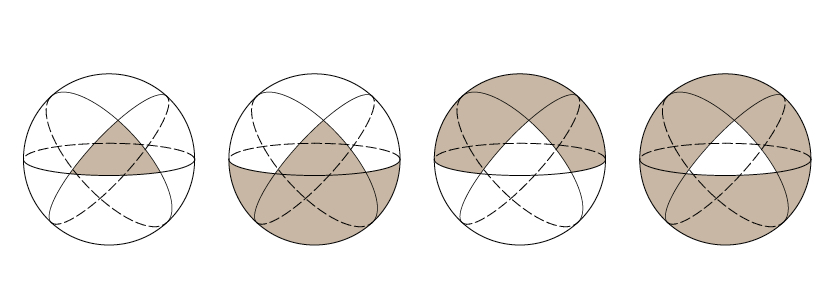
\includegraphics[width=0.9\textwidth]{kugel/Dreieckarten.jpg}
    \captionof{figure}{Dreieckarten auf einer Kugeloberfläche}
\end{center}

Der Begriff Sphärisches Dreieck oder Kugeldreieck ist ein sehr weitläufiger Begriff. 
Dabei können wir den Begriff in drei für uns wesentliche Dreiecke unterteilen:

\begin{itemize}
\item Kugelzweieck
\item Nicht Eulersche’Dreiecke
\item Eulersche’Dreiecke
\end{itemize}

\subsection{Kugelzweieck}

Zwei Grosskreise auf der Kugeloberfläche, zerlegen diese in vier gleiche Kugelzweiecke. 
Jedes dieser Dreieckseiten hat die Länge
$180^{\circ}$ oder $\pi$
Der Flächeninhalt wird dabei nur durch den Winkel $\alpha$ zwischen den beiden Grosskreisen bestimmt.

\begin{center}
        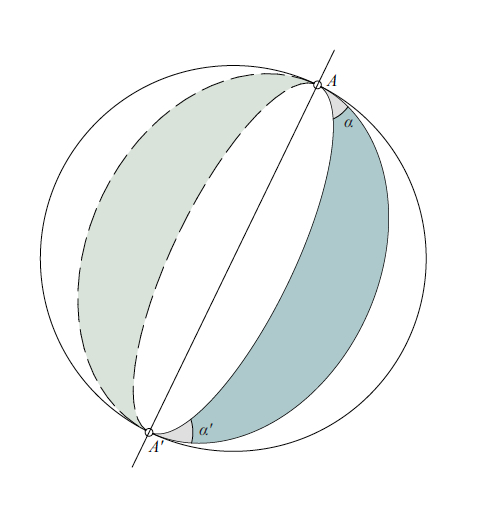
\includegraphics[width=0.3\textwidth]{kugel/Zweieck.jpg}
    \captionof{figure}{Bildung von Zweiecken durch Grosskreise}
\end{center}

Dabei ist der Flächeninhalt der ganzen Kugel:

\begin{align*}
A_{ Kugel } &= 4 \pi r^{2}
\end{align*}


Um den Flächeninhalt des betrachteten Zweieckes zu bekommen, 
müssen wir das ganze noch mit dem Kugelsegment mit dem Winkel $\alpha$ multiplizieren.

\begin{align*}
A_{ Zweieck } &= 4 \pi r^{2} \cdot \frac{ \alpha }{ 2 \pi }
\end{align*}


\subsection{Nicht Eulersche’ Dreiecke}

BLABLA

\subsection{Eulersche’ Dreiecke}

Legt man drei Grosskreise auf eine Kugeloberfläche, bilden sich dabei acht Dreiecke. 
Ein solches Dreieck heisst Eulersches’Dreieck\footnote{%
Leonard Euler (1707-1783), berühmter Schweizer Mathematiker und Physiker. 
Nicht Eulersche’Dreiecke erhält man, indem man das Äussere des Dreieckes ABC betrachtet.} 
Diese Dreiecke werden weder durch die Verlängerung ihrer Seiten durchschnitten, 
noch haben sie Dreiecksseiten welche grösser als $180^{\circ}$ sind.

\begin{center}
        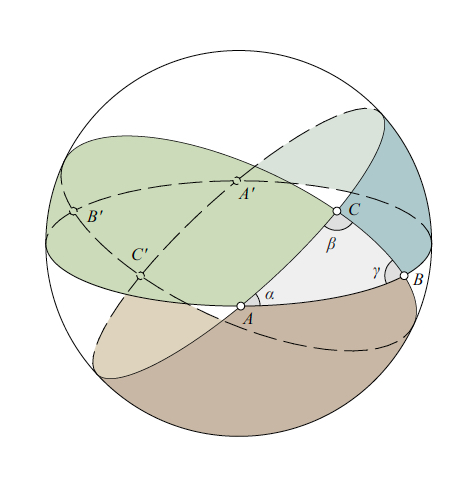
\includegraphics[width=0.4\textwidth]{kugel/Zweiecke.jpg}
    \captionof{figure}{Drei Grosskreise bilden ein sphärisches Dreieck}
\end{center}

In den nachstehenden Erklärungen und Herleitungen, sprechen wir ausschliesslich von Eulerschen’Dreiecken, da die umgeformten Winkelsätze der ebenen Trigonometrie nur auf diese Art von Kugeldreiecken angewendet werden kann.

$A_{ \overline{ ABC }}$ ist die Fläche des Dreieckes auf der Kugeloberfläche
In der ebenen Trigonometrie liegt die Winkelsumme eines Dreiecks bei
$180^{\circ}$.

Anders aber in der sphärischen Trigonometrie. Obschon sie einige Gemeinsamkeiten zur ebenen Trigonometrie aufweist, kann man nicht alles übernehmen.
So auch nicht wie Winkelsumme in einem sphärischen Dreieck.
Diese liegt bei:

\[
\begin{aligned}
\pi
&-
3\pi
&
&\text{\bigg \vert}
&
180^{\circ}
&-
540^{\circ}
\end{aligned}
\]

daraus lässt sich ableiten, das ein einzelner Winkel nicht grösser als $\pi$ oder $180^{\circ}$ sein darf. Ansonsten ist es kein Eulersches’Dreieck und wir dürfen die sphärische Trigonometrie nicht anwenden.\\
Wichtig anzumerken ist, dass die Seiten immer in Radiant beschrieben werden und nicht im Längenmass Meter wie wir es uns gewohnt sind. 
Bei den Dreiecksseiten handelt es sich um Kreisbögen und keine Strecken.

\section{Dreiecksfläche}

\begin{align*}
\text{Zweieck A}
&=
\overline{ABC} + \overline{A'BC} = 2 \alpha r^{ 2 } = A_{ \alpha }\\
\text{Zweieck B}
&=
\overline{ABC} + \overline{AB'C} = 2 \beta r^{ 2 } = A_{ \beta }\\
\text{Zweieck C}
&=
\overline{ABC} + \overline{ABC'} = 2 \gamma r^{ 2 } = A_{ \gamma }
\end{align*}

\begin{align*}
A_{ \alpha } + A_{ \beta } + A_{ \gamma } &= \frac{ 4\pi r^{ 2 } }{ 2 } + 2A_{ \overline{ ABC }} \\
2\alpha r^{ 2 } + 2\beta r^{ 2 } + 2\gamma r^{ 2 } &= \frac{ 4\pi r^{ 2 } }{ 2 } + 2A_{ \overline{ ABC }} \parallel:2\\
\alpha r^{ 2 } + \beta r^{ 2 } + \gamma r^{ 2 } &= \pi r^{ 2 } + A_{ \overline{ ABC }} \parallel-\pi r^{ 2 }\\
r^{ 2 }\left(\alpha + \beta + \gamma - \pi\right) &= A_{ \overline{ ABC }}
\end{align*}




\section{Sphärischer Exzess}
Die Winkelsumme sphärischer Dreiecke ist immer \textgreater \,  $\pi$.

\begin{align*}
\pi < \alpha + \beta + \gamma
\end{align*}

Der sphärische Exzess gibt dabei an, wie stark die Winkelsumme von $\pi$ abweicht.

\begin{align*}
\pi + \epsilon &= \alpha + \beta + \gamma \\
\epsilon &= \alpha + \beta + \gamma - \pi
\end{align*}

Würde der sphärische Exzess in der ebenen Trigonometrie angewendet, wäre dieser = 0. 
Bezieht man das auf die Erde und somit einer Kugel, kann man mit Hilfe eines beliebigen sphärischen Dreieckes und dessen Flächeninhalt auf den Radius der Kugel schliessen.

\subsection{Grenzfall - Satz von Legendre}

\begin{quote} \textit{Ein kleines sphärisches Dreieck kann näherungsweise 
wie ein ebenes Dreieck mit denselben Seiten berechnet 
werden, wenn alle Winkel des ebenen Dreiecks die um 
je ein Drittel des sphärischen Exzesses verminderten 
Winkel des sphärischen Dreiecks nimmt.} \end{quote}
\begin{flushright} - Adrien-Marie Legendre (1752-1833), Paris 1787
\end{flushright}x

Diese Aussage zeigt den Zusammenhang zwischen der 
Trigonometrie in der Ebene sowie in auf der Kugel
auf. Im speziellen bei sehr kleinen sphärischen 
Dreiecken ist die Winkelsumme nur unwesentlich 
grösser als $180^{\circ}$. Des Weiteren kann gesagt werden,
dass der sphärische Exzess gleichmässig auf alle
Winkel aufgeteilt wird.
Wichtig anzumerken ist, dass der Satz von Legendre 
für grosse, aber endliche Radien $r$ gilt.

%[SKIZZE GROSSER RADIUS/KLEINE KRÜMMUNG, KLEINER RADIUS/GROSSE KRÜMMUNG!!!!]
%


\section{Sphärisch Analoge Winkelfunktionen}

\subsection{Sphärischer Sinussatz}

Wir stellen die allgemeinen Sinussätze der Winkel $\alpha$ und $\gamma$ auf:


\[
\begin{aligned}
&{sin(\gamma)} = \frac{h}{a}
&
&\text{\bigg \vert}
&
&{sin(\alpha)} = \frac{h}{c}
&
\end{aligned}
\]

Daraus folgt:
\begin{align*}
h &= sin(\gamma)\cdot a \\
h &= sin(\alpha)\cdot c
\end{align*} 

Durch Gleichsetzung erhält man:
\begin{align*}
h &= h \\
sin(\gamma)\cdot a &= sin(\alpha)\cdot c
\end{align*} 

Durch umstellen erhalten wir den Sinussatz für a und c:
\begin{align*}
sin(\gamma)\cdot a &= sin(\alpha)\cdot c \\
\frac{sin(\gamma)}{c} &= \frac{sin(\alpha)}{a} 
\end{align*} 



\begin{align*}
\frac{sin(\alpha)}{sin(a)} = \frac{sin(\beta)}{sin(b)} = \frac{sin(\gamma)}{sin(c)}
\end{align*} 


\subsection{Winkelkosinussatz}

%[SKIZZE WINKELKOSINUS]

\[
\begin{aligned}
&\overline{C'A'} &= d\cdot {tan(b)}
&
&
&
&
&
&\overline{C'B'} &= d\cdot {tan(a)}
\end{aligned}
\]

\[
\begin{aligned}
&\overline{MA'} &= \frac{ d }{cos(b)}
&
&
&
&
&
&\overline{MB'} &= \frac{ d }{cos(a)}
\end{aligned}
\]

Der allgemeine Kosinussatz beschreibt sich wie folgt:

\begin{align*}
c^{ 2 } &= a^{ 2 } + b^{ 2 } - 2ab \cdot cos(\gamma)
\end{align*}

\begin{align*}
\triangle \overline{A'B'C' }
\overline{ A'B' }^{ 2 } &= \overline{ C'B' }^{ 2 } + \overline{ C'A' }^{ 2 } - 2 \cdot \overline{ C'B' } \cdot \overline{ C'A' } \cdot cos(\gamma)
\end{align*}



\begin{align*}
\overline{A'B'}^{ 2 } &= (d\cdot tan(a))^{ 2 } + (d\cdot tan(b))^{ 2 } - 2 \cdot (d\cdot tan(a) \cdot (d\cdot tan(b) \cdot cos(\gamma)\\
\overline{A'B'}^{ 2 } &= d^{ 2 } \cdot \left(\left(tan^{ 2 }(a) + tan^{ 2 }(b)\right) - 2\cdot tan(a) \cdot tan(b) \cdot cos(\gamma)\right)
\end{align*}

\begin{align*}
\triangle \overline{ MA'B' }
\overline{ A'B' }^{ 2 } &= \overline{ MB' }^{ 2 } + \overline{ MA' }^{ 2 } - 2\cdot \overline{ MB'} \cdot \overline{ MA' } \cdot cos(c)
\end{align*}


\begin{align*}
\overline{ A'B'}^{ 2 } &= \left(\frac{ d }{ cos(a) }  \right)^{ 2 } + \left(\frac{ d }{ cos(b)}  \right)^{ 2 } - 2 \cdot \frac{ d }{ cos(a)} \cdot \frac{ d }{ cos(b)} \cdot cos(c) \\
\overline{ A'B' }^{ 2 } &= d^{ 2 } \cdot \left(\left(\frac{ 1 }{ cos(a) }  \right)^{ 2 } + \left(\frac{ 1 }{ cos(b) }  \right)^{ 2 } - 2 \cdot \frac{ 1 }{ cos(a)} \cdot \frac{ 1 }{ cos(b)} \cdot cos(c)\right)\\
\overline{ A'B' }^{ 2 } &= d^{ 2 } \cdot \left(\left(tan^{ 2 }(a) + 1\right) + \left(tan^{ 2 }(b) + 1\right) - \left(2 \cdot \frac{cos(c)}{cos(a) \cdot cos(b)}\right)\right)
\end{align*}



\begin{align*}
\overline{ A'B'}^{ 2 } &= d^{ 2 } \cdot \left(\left(tan^{ 2 }(a) + tan^{ 2 }(b)\right) - 2 \cdot tan(a) \cdot tan(b) \cdot cos(\gamma)\right) \\
\overline{ A'B'}^{ 2 } &= d^{ 2 } \cdot \left(\left(tan^{ 2 }(a) + 1\right) + \left(tan^{ 2 }(b) + 1\right) - \left(2 \cdot \frac{cos(c)}{cos(a) \cdot cos(b)}\right)\right)
\end{align*}

Die anderen Gleichungen des Satzes, erfolgen aus Symmetriegründen.

\subsection{Seitenkosinussatz}
Durch zyklische Vertauschung des Winkelkosinus erhalten wir den Seitenkosinussatz:

\begin{align*}
{cos(a)} &= {cos(b)} \cdot {cos(c)} + {sin(b)} \cdot {sin(c)} \cdot {sin(\alpha)}\\
{cos(b)} &= {cos(a)} \cdot {cos(c)} + {sin(a)} \cdot {sin(c)} \cdot {sin(\beta)}\\
{cos(c)} &= {cos(a)} \cdot {cos(b)} + {sin(a)} \cdot {sin(b)} \cdot {sin(\gamma)}\\
\end{align*}

\section{Navigation auf See}
Das besondere an Seekarten ist die Inhaltliche Ausrichtung. Anders wie Landkarten muss sie Informationen enthalten welche für den Kapitän und seine Besatzung von grosser Bedeutung sind. Vor allem in Küstennähe ist das navigieren eines Schiffes besonders gefährlich. So enthalten Seekarten etwas über Wassertiefen, Bodenbeschaffenheiten, Gezeiten, Küstenlinien, Landzungen und Windrichtungen.
Der Hauptunterschied dabei ist, das auf der Landkarte feste Positionen definiert und aufgezeigt werden, das einzige was sich verändert ist der Reisende selbst. Bei der Seekarte ist das anders, es werden veränderliche Einwirkungen der Natur festgehalten.

Dieser kleine Unterschied zeigt die Notwendigkeit auf, die Position und den Kurs seines Schiffes auf See immer ermitteln zu können.


\section{Geographische Koordinaten}

Nachdem klar war, das die Erde eine Kugel ist, wurde diese in ein Gradnetz aufgeteilt. Dabei wurden die Angaben für eine exakte Ortsbestimmung klar definiert und die bis heute gültigen Koordinaten bestimmt.
Dabei muss man sich nochmals in Erinnerung rufen, dass sich die Erde in 24h einmal um ihre eigene Achse dreht. Nach $360 ^{\circ}$ 
und somit einer vollen Umdrehung, steht sie wieder in ihrer Ursprungsposition und ein neuer Tag beginnt.

Die Koordinaten setzen sich aus folgenden Komponenten zusammen:

\[
\begin{aligned}
&\text{Grad } (^{\circ})
&
&\text{\bigg \vert}
&
&\text{Bogenminuten } (`)
&
&\text{\bigg \vert}
&
&\text{Bogensekunden } (``)
\end{aligned}
\]

Die Erdoberfläche wurde in je 360 Breiten- und Längengrade eingeteilt. Die Breitengrade haben zueinander einen Abstand von 111.31 km, dies entspricht auch dem Abstand der Längengrade am Äquator mit Zunehmender Nähe zu den Polen, nimmt dieser Abstand ab.

\[
\begin{aligned}
&1^{\circ}
&
&\text{\bigg \vert}
&
&4 \text{ Minuten}
&
&\text{\bigg \vert}
&
&111.31\text{ km}
\end{aligned}
\]

Berechnet man nun die Erdumdrehung von 360°, erhält man genau den Erdumfang am Äquator: \begin{align*} 40’074 \text{ km.}\end{align*}

Dabei geben die Bogenminuten und -sekunden dem Standort die gewünschte Exaktheit. Mit den vollständigen Koordinaten lässt sich der Standort auf einer Landkarte exakt bestimmen und einzeichnen.

\subsection{Zeitzonen der Erde}
Wenn man nun die verschiedenen Zeitzonen der Erde betrachtet, macht die Verschiebung von jeweils einer Stunde durchaus Sinn, es lässt sich auf die Längengrade schliessen.
Zwischen den verschiedenen Zeitzonen liegen 15 Längengrade:

\begin{align*}
\text{15 Längengrade à 4 Minuten = 60 Minuten Zeitverschiebung = ca. 1665 km}
\end{align*}

Dabei ist die Zeitzone in welcher Mitte sich der Greenwich Meredian befindet die \textit{Greenwich Mean Time (GMT)} welche bis 1928 als Weltzeit galt. Im Jahr 1972 wurde diese umbenannt in die \textit{Coordinated Universal Time (UTC)} und wir von da an als Weltzeit $\pm$ 0.00 verwendet.


\section{Der Breitengrad}
Die Breitengrade bilden die bereits genannten Kleinkreise auf der Kugeloberfläche. Sie verlaufen in einem Abstand von genau 111 km parallel zum Äquator. Dabei stellt  dieser genau die Mitte zwischen Nord- und Südpol dar und teilt die Erdkugel in zwei gleiche Hälften. Somit wird von nördlicher und südlicher Breite gesprochen, je nach dem auf welcher Halbkugel man sich befindet.

%[SKIZZE DER GEOGRAFISCHEN BREITE ERDKUGEL]

\subsection{Geografische Breite $\phi$}
\begin{definition}
Die geografische Breite eines Standortes ist nichts anderes, als der Winkel am Erdmittelpunkt zwischen der Ebene des Äquators und der Geraden zum Standpunkt auf der Erdoberfläche.
\end{definition}

%[SKIZZE DER GEOGRAFISCHEN BREITE MIT WINKEL]

\subsection{Navigation mit den Breitengraden}
Da der Breitengrad bereits sehr früh ziemlich präzise bestimmt werden könnte, nutzten bereits die Seefahrer um Christoph Kolumbus den Breitengrad zur Navigation ihrer Flotten.
Den dieser lässt sich ziemlich einfach aus dem höchsten Sonnenstand oder einem Fixstern bestimmen. Dabei wird mit einem Jakobsstab\footnote{%
Der Jakobsstab ist ein früheres astronomisches Instrument zur Winkelmessung und wurde vor allem in der Seefahrt verwendet. Er ist in der Nautik der Vorläufer des Sextanten.} (später Sextant\footnote{%
Der Sextant ist ein nautisches Messinstrument zur Winkelmessung von Horizont und Fixstern (Gestirn)}) der Winkel zwischen dem Horizont und dem Fixstern gemessen. Der Winkel welchen man erhält, zieht man von 90° ab und erhält somit die geografische Breite. \\

%[SKIZZE ERMITTLUNG DES BREITENGRADES]

Wenn man sich auf der Nordhalbkugel befindet, ist der Polarstern ein sehr guter Fixstern. Befindet sich ein Schiff nun sehr nahe am Nordpol, steht dieser nahezu senkrecht am Himmelszelt bei $90^{\circ}$. Würde es aber nahe dem Äquator stehen, erscheint dieser am Horizont bei $0^{\circ}$.

\subsection{Korrekturbeiwert}

\section{Der Längengrad}
Die Längengrade bilden die bereits genannten Grosskreise auf der Kugeloberfläche.
Sie schneiden den Äquator im rechten Winkel, haben dort einen Abstand von 111 km zueinander und verbinden die Pole. Anders wie bei der geografischen Breite, ist in der Natur kein Längengrad gegeben welcher den Nullpunkt darstellt.

%[SKIZZE DER GEOGRAFISCHEN LÄNGE ERDKUGEL]

\subsection{Geografische Länge $\lambda$}
\begin{definition}
Die geografische Länge ist der Winkel an der Erdachse zum Nullmeridian.
\end{definition}

\subsection{Navigation mit den Längengraden}
Die geografische Länge lässt sich nicht so einfach bestimmen wie deren Breite. Für die Berechnung auf See benötigt man eine Referenzzeit eines Ortes mit bekannter Länge.
In der Zeit der Entdecker gab es noch keine mechanischen Uhren. Die Sonnenuhr war zudem ungeeignet, da diese nur die Uhrzeit am Standort mass und nicht die am Referenzort selbst. Die erste Pendeluhr wurde erst Mitte des 17. Jahrhunderts erfunden, was in der Schifffahrt aber auch nicht die Lösung brachte.\\
Pendeluhren auf einem Schiff sind ungeeignet, da das Pendel mit dem Wellengang aus dem Takt gebracht wird und somit die Uhr falsch geht.
Zu ungenau und gegen äussere Erschütterungen zu empfindlich waren später auch die federgetriebenen Uhren und die Unruh. Dazukamen die verschiedenen Klimazonen welche ein Schiff zu durchqueren hatten. Das Metall zog sich viel zu fest zusammen oder dehnte sich aus, was dazu führte das die Uhr unregelmässig lief.

Das sogenannte „Längenproblem“ stellte nicht nur bei der Navigation auf See ein Problem dar, es ergaben sich auch wirtschaftliche Konsequenzen. Die Schiffe mussten bis zur gewünschten geografischen Breite navigieren und segelten dann den Breitengrad entlang. Dabei waren die Schiffe oft Wochenlang unterwegs und segelten die „Breiten ab“ um an die gewünschte Position zu kommen. Dies führte zu erheblichen Zeitverlusten und viel längeren Reisezeiten.


\section{The Board of Longitude - Das Längenproblem}
Das Längenproblem beschäftigte alle grossen Seefahrernationen Europas. Wenn man bedenkt das sich Werte in einer  Höhe von halben britischen Staatshaushalten auf verloren gegangenen Schiffen befanden, erkennt man die Dringlichkeit für eine zuverlässige und genaue Navigation auf See.


\begin{itemize}
\item £ 20’000 - Abweichung von max. einem halben Grad
\item £ 15’000 - Abweichung von zwei Drittel Grad
\item £ 10’000 - Abweichung von max. $1 ^{\circ}$
\end{itemize}

\subsection{John Harrison}


\subsection{Tobias Mayer}



Uhren mit einer Abweichung von einer Minute Abweichung pro Tag (





\section{Nautische Dreieck}


$\Rightarrow$





\section{Die Vermessung der Welt}
Wir schreiben das Jahr 1818 und kehren in die Zeit des Mathematikers Carl Friedrich Gauss zurück. Neben dem liebevoll genannten „kleinen Gauss“ und anderen herausragenden Mathematischen Leistungen, beschäftigte er in den Folgejahren mit der Vermessung des Königreichs Hannovers und verfasste auf 61 Blättern das Kartenwerk \textit{Gauss’sche Landesaufnahme der 1815 durch Hannover erworbenen Gebiete}.






AUFGABE

Hubble Teleskop 
24. April 1990






\printbibliography[heading=subbibliography]
\end{refsection}




%\chapter{Geometrie auf der Kugeloberfläche\label{chapter:kugel}}
\lhead{Geometrie auf der Kugeloberfläche}
\begin{refsection}
\chapterauthor{Melina Staub und Fabian Schmid}

\section{Einleitung}

Schon seit jeher fasziniert den Menschen die Fahrt zur See. Nicht grundlos ist die Seefahrt eine der wichtigsten und ältesten Tätigkeiten der Menschheit. Der innerliche Drang neue Weltmeere und unbekannte Gebiete zu entdecken, die Fahrt zur See zu erleichtern und erträglicher zu machen, trieben die Menschen an, die Schiffe dieser Welt immer weiter zu entwickeln.

Die Idee der Kugelform der Erde ist älter als man zu denken vermag. Bereits der Schüler des antiken griechischen Philosophen Platon - Aristoteles schrieb in seiner Schrift \textit{Über den Himmel} aus dem 4. Jahrhundert v. Chr. etliche Gründe welche für die Gestallt der Erde als Kugel sprechen:

\begin{itemize}
      \item Sämtliche schweren Körper streben zum Mittelpunkt des Alls. Da sie dies von allen Seiten her gleichmäßig tun und die Erde im Mittelpunkt des Alls steht, muss sie eine kugelrunde Gestalt annehmen. 
\item Bei von der Küste wegfahrende Schiffen wird der Rumpf vor den Segeln der Sicht verborgen. 
\item In südlichen Ländern erscheinen südliche Sternbilder höher über dem Horizont.
\item Der Erdschatten bei einer Mondfinsternis ist stets rund.
\end{itemize}

Jedoch war um 1492 - der Zeit der Entdeckung Amerikas durch Christoph Kolumbus, die Idee der Erde in Kugelform noch sehr umstritten. Er erkannte anhand den Theorien und Erkenntnissen der alten Griechen, vor allem Aristoteles, das die Erde eine Kugel sein muss. \\
Doch mit seinem Vorschlag einen Seeweg über den Atlantik nach Indien zu finden und nicht wie üblich um Afrika zu segeln, stiess er beim beim portugiesischen König auf taube Ohren. Sein Plan Indien über eine Route nach Westen zu erreichen, widersprach dem gesunden Menschenverstand. Wäre die Erde wirklich eine Kugel und man befände sich auf der unteren Erdhalbkugel, würde man herunterfallen.\\
Doch auch der damals übliche Glaube an die Erde in Scheibenform brachte so einige Risiken mit sich. Was würde passieren, wenn die Flotte das Ende der Scheibe erreicht hatte? Würden sie über den Erdrand hinweggleiten und in den Abgrund stürzen?\\
Erst nach viel Überzeugungsarbeit durch Kolumbus, setzte er sich am Spanischen Hof durch und segelte über die Westliche Route über den Atlantik und entdeckte schlussendlich Amerika.

Der praktische und greifbare Beweis das die Erde eine Kugel ist, lieferte rund 30 Jahre später der Portugiese Fernando Magellan. Mit seiner Weltumsegelung und seiner Ankunft in den Philippinen, bewies er definitiv das die Erde eine Kugel ist.\\

Nun wollen wir uns die Frage stellen, wie die alten Seefahrer ohne GPS und jeglichen modernen Navigationssystemen auf hoher See wussten wo sie sich befinden und was haben die Sterne mit alldem zu tun? Reisen Sie mit uns zurück in eine Zeit mit Sextant, Kompass und Sternkarten. In die Zeit der Seefahrer und Entdecker.


\section{Geometrie auf der Ebene und der Kugel}

Euklid von Alexandria beschrieb die Grundbegriffe der ebenen Geometrie mittels Punkt, Geraden, Ebene, Winkel und Dreieck. Diese Dreiecke lassen sich mithilfe der ebenen Trigonometrie beschreiben. Dabei gelten die uns bekannten trigonometrischen Winkelfunktionen:\\

\text{Sinussatz:}
\begin{align*}
\frac{ a }{ sin(\alpha) } &= \frac{ b }{sin(\beta)} = \frac{ c }{ sin(\gamma) } = \frac{abc}{2A} = 2r\\
\end{align*}

\text{Cosinussatz:}
\begin{align*}
c^{ 2 } &= a^{ 2 } + b^{ 2 } - 2ab\cdot cos(\gamma)\\
b^{ 2 } &= a^{ 2 } + c^{ 2 } - 2ab\cdot cos(\beta)\\
a^{ 2 } &= b^{ 2 } + c^{ 2 } - 2ab\cdot cos(\alpha)
\end{align*}

Um Dreiecke auf der Kugeloberfläche zu berechnen, benötigt man die sphärische Trigonometrie. Die oben beschriebenen Sätze lassen sich auf der Kugel nicht anwenden, sie werden aber als Grundlage zur Herleitung der Sätze für das Kugeldreieck benötigt.

Die nachfolgenden Seiten thematisieren die Geometrie auf der Kugeloberfläche und wie sie in der Navigation eingesetzt werden kann.


\section{Gross- und Kleinkreise}

Eine Kugeloberfläche lässt sich in zwei verschiedene Kreisarten einteilen -  Gross- und Kleinkreise. 
Wir betrachten als erstes die Grosskreise:

\begin{definition}
Ein Großkreis ist ein größtmöglicher Kreis auf einer Kugeloberfläche. Sein Mittelpunkt fällt immer mit dem Mittelpunkt der Kugel zusammen und ein Schnitt auf dem Großkreis teilt die Kugel in jedem Fall in zwei („gleich große“) Hälften.
\end{definition}

Es gibt unendlich viele Möglichkeiten, eine Kugel in zwei gleich grosse Stücke zu zerschneiden, 
daher gibt es auch unendlich viele Grosskreise. Wenn wir die Grosskreise auf einer Kugel mit diesen auf der Erde beschreiben, sprechen wir von den Längengraden aber auch der Äquator beschreibt einen Grosskreis.
Ein Elementarer Bestandteil bilden die Grosskreise in der sphärischen Trigonometrie. Mithilfe der Schnittpunkte verschiedener Grosskreise, lässt sich ein Sphärisches Dreieck bilden auf welchem sich die sphärische Trigonometrie anwenden lässt.

[GRAFIK GROSSKREISE]

\begin{definition}
Unter Kleinkreis versteht man jene Kreise auf einer Kugeloberfläche, deren Ebenen nicht den Kugelmittelpunkt enthalten.
\end{definition}

Die Kleinkreise eignen sich im Gegensatz zu den Grosskreisen \textit{nicht} für die sphärische Trigonometrie. 
Sie werden lediglich zur Bestimmung der Messgrössen, Winkelabstände oder des Höhenwinkels eines Gestirns verwendet. 

Wenn wir die Kleinkreise auf die Erdoberfläche projizieren betrachten wir die Breitengrade.

[GRAFIK KLEINKREISE]


\section{Sphärische Dreiecke / Kugeldreieck}

\begin{center}
        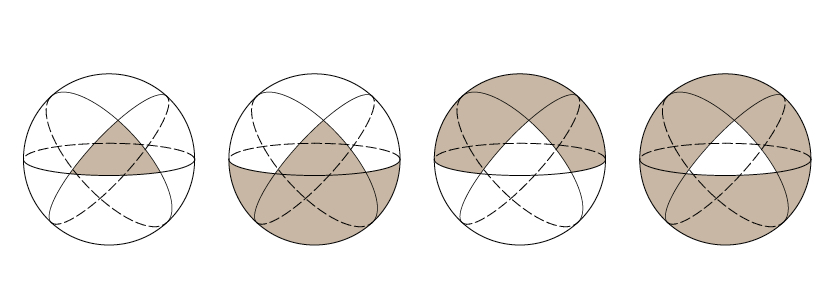
\includegraphics[width=0.9\textwidth]{kugel/Dreieckarten.jpg}
    \captionof{figure}{Dreieckarten auf einer Kugeloberfläche}
\end{center}

Der Begriff Sphärisches Dreieck oder Kugeldreieck ist ein sehr weitläufiger Begriff. 
Dabei können wir den Begriff in drei für uns wesentliche Dreiecke unterteilen:

\begin{itemize}
\item Kugelzweieck
\item Nicht Eulersche’Dreiecke
\item Eulersche’Dreiecke
\end{itemize}

\subsection{Kugelzweieck}

Zwei Grosskreise auf der Kugeloberfläche, zerlegen diese in vier gleiche Kugelzweiecke. 
Jedes dieser Dreieckseiten hat die Länge
$180^{\circ}$ oder $\pi$
Der Flächeninhalt wird dabei nur durch den Winkel $\alpha$ zwischen den beiden Grosskreisen bestimmt.

\begin{center}
        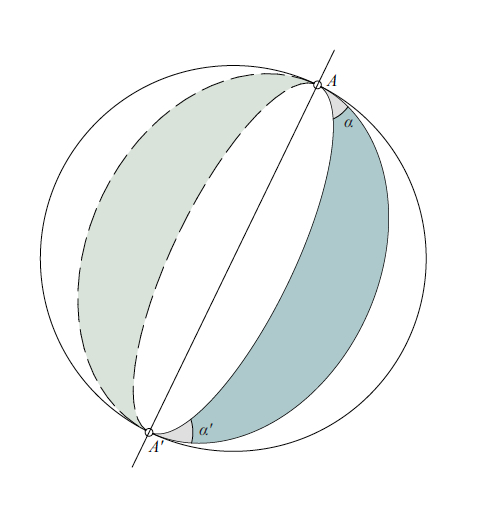
\includegraphics[width=0.3\textwidth]{kugel/Zweieck.jpg}
    \captionof{figure}{Bildung von Zweiecken durch Grosskreise}
\end{center}

Dabei ist der Flächeninhalt der ganzen Kugel:

\begin{align*}
A_{ Kugel } &= 4 \pi r^{2}
\end{align*}


Um den Flächeninhalt des betrachteten Zweieckes zu bekommen, 
müssen wir das ganze noch mit dem Kugelsegment mit dem Winkel $\alpha$ multiplizieren.

\begin{align*}
A_{ Zweieck } &= 4 \pi r^{2} \cdot \frac{ \alpha }{ 2 \pi }
\end{align*}


\subsection{Nicht Eulersche’ Dreiecke}

BLABLA

\subsection{Eulersche’ Dreiecke}

Legt man drei Grosskreise auf eine Kugeloberfläche, bilden sich dabei acht Dreiecke. 
Ein solches Dreieck heisst Eulersches’Dreieck\footnote{%
Leonard Euler (1707-1783), berühmter Schweizer Mathematiker und Physiker. 
Nicht Eulersche’Dreiecke erhält man, indem man das Äussere des Dreieckes ABC betrachtet.} 
Diese Dreiecke werden weder durch die Verlängerung ihrer Seiten durchschnitten, 
noch haben sie Dreiecksseiten welche grösser als $180^{\circ}$ sind.

\begin{center}
        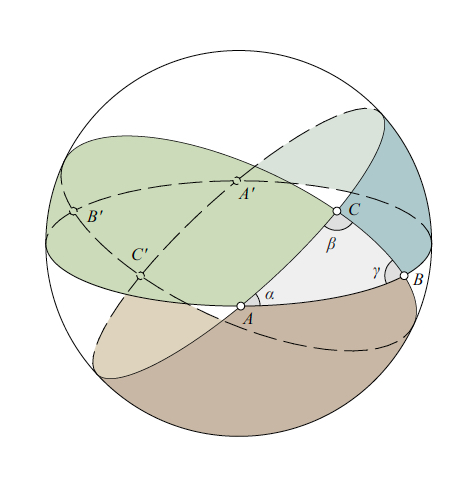
\includegraphics[width=0.4\textwidth]{kugel/Zweiecke.jpg}
    \captionof{figure}{Drei Grosskreise bilden ein sphärisches Dreieck}
\end{center}

In den nachstehenden Erklärungen und Herleitungen, sprechen wir ausschliesslich von Eulerschen’Dreiecken, da die umgeformten Winkelsätze der ebenen Trigonometrie nur auf diese Art von Kugeldreiecken angewendet werden kann.

$A_{ \overline{ ABC }}$ ist die Fläche des Dreieckes auf der Kugeloberfläche
In der ebenen Trigonometrie liegt die Winkelsumme eines Dreiecks bei
$180^{\circ}$.

Anders aber in der sphärischen Trigonometrie. Obschon sie einige Gemeinsamkeiten zur ebenen Trigonometrie aufweist, kann man nicht alles übernehmen.
So auch nicht wie Winkelsumme in einem sphärischen Dreieck.
Diese liegt bei:

\[
\begin{aligned}
\pi
&-
3\pi
&
&\text{\bigg \vert}
&
180^{\circ}
&-
540^{\circ}
\end{aligned}
\]

daraus lässt sich ableiten, das ein einzelner Winkel nicht grösser als $\pi$ oder $180^{\circ}$ sein darf. Ansonsten ist es kein Eulersches’Dreieck und wir dürfen die sphärische Trigonometrie nicht anwenden.\\
Wichtig anzumerken ist, dass die Seiten immer in Radiant beschrieben werden und nicht im Längenmass Meter wie wir es uns gewohnt sind. 
Bei den Dreiecksseiten handelt es sich um Kreisbögen und keine Strecken.

\section{Dreiecksfläche}

\begin{align*}
\text{Zweieck A}
&=
\overline{ABC} + \overline{A'BC} = 2 \alpha r^{ 2 } = A_{ \alpha }\\
\text{Zweieck B}
&=
\overline{ABC} + \overline{AB'C} = 2 \beta r^{ 2 } = A_{ \beta }\\
\text{Zweieck C}
&=
\overline{ABC} + \overline{ABC'} = 2 \gamma r^{ 2 } = A_{ \gamma }
\end{align*}

\begin{align*}
A_{ \alpha } + A_{ \beta } + A_{ \gamma } &= \frac{ 4\pi r^{ 2 } }{ 2 } + 2A_{ \overline{ ABC }} \\
2\alpha r^{ 2 } + 2\beta r^{ 2 } + 2\gamma r^{ 2 } &= \frac{ 4\pi r^{ 2 } }{ 2 } + 2A_{ \overline{ ABC }} \parallel:2\\
\alpha r^{ 2 } + \beta r^{ 2 } + \gamma r^{ 2 } &= \pi r^{ 2 } + A_{ \overline{ ABC }} \parallel-\pi r^{ 2 }\\
r^{ 2 }\left(\alpha + \beta + \gamma - \pi\right) &= A_{ \overline{ ABC }}
\end{align*}




\section{Sphärischer Exzess}
Die Winkelsumme sphärischer Dreiecke ist immer \textgreater \,  $\pi$.

\begin{align*}
\pi < \alpha + \beta + \gamma
\end{align*}

Der sphärische Exzess gibt dabei an, wie stark die Winkelsumme von $\pi$ abweicht.

\begin{align*}
\pi + \epsilon &= \alpha + \beta + \gamma \\
\epsilon &= \alpha + \beta + \gamma - \pi
\end{align*}

Würde der sphärische Exzess in der ebenen Trigonometrie angewendet, wäre dieser = 0. 
Bezieht man das auf die Erde und somit einer Kugel, kann man mit Hilfe eines beliebigen sphärischen Dreieckes und dessen Flächeninhalt auf den Radius der Kugel schliessen.

\subsection{Grenzfall - Satz von Legendre}

\begin{quote} \textit{Ein kleines sphärisches Dreieck kann näherungsweise 
wie ein ebenes Dreieck mit denselben Seiten berechnet 
werden, wenn alle Winkel des ebenen Dreiecks die um 
je ein Drittel des sphärischen Exzesses verminderten 
Winkel des sphärischen Dreiecks nimmt.} \end{quote}
\begin{flushright} - Adrien-Marie Legendre (1752-1833), Paris 1787
\end{flushright}x

Diese Aussage zeigt den Zusammenhang zwischen der 
Trigonometrie in der Ebene sowie in auf der Kugel
auf. Im speziellen bei sehr kleinen sphärischen 
Dreiecken ist die Winkelsumme nur unwesentlich 
grösser als $180^{\circ}$. Des Weiteren kann gesagt werden,
dass der sphärische Exzess gleichmässig auf alle
Winkel aufgeteilt wird.
Wichtig anzumerken ist, dass der Satz von Legendre 
für grosse, aber endliche Radien $r$ gilt.

%[SKIZZE GROSSER RADIUS/KLEINE KRÜMMUNG, KLEINER RADIUS/GROSSE KRÜMMUNG!!!!]
%


\section{Sphärisch Analoge Winkelfunktionen}

\subsection{Sphärischer Sinussatz}

Wir stellen die allgemeinen Sinussätze der Winkel $\alpha$ und $\gamma$ auf:


\[
\begin{aligned}
&{sin(\gamma)} = \frac{h}{a}
&
&\text{\bigg \vert}
&
&{sin(\alpha)} = \frac{h}{c}
&
\end{aligned}
\]

Daraus folgt:
\begin{align*}
h &= sin(\gamma)\cdot a \\
h &= sin(\alpha)\cdot c
\end{align*} 

Durch Gleichsetzung erhält man:
\begin{align*}
h &= h \\
sin(\gamma)\cdot a &= sin(\alpha)\cdot c
\end{align*} 

Durch umstellen erhalten wir den Sinussatz für a und c:
\begin{align*}
sin(\gamma)\cdot a &= sin(\alpha)\cdot c \\
\frac{sin(\gamma)}{c} &= \frac{sin(\alpha)}{a} 
\end{align*} 



\begin{align*}
\frac{sin(\alpha)}{sin(a)} = \frac{sin(\beta)}{sin(b)} = \frac{sin(\gamma)}{sin(c)}
\end{align*} 


\subsection{Winkelkosinussatz}

%[SKIZZE WINKELKOSINUS]

\[
\begin{aligned}
&\overline{C'A'} &= d\cdot {tan(b)}
&
&
&
&
&
&\overline{C'B'} &= d\cdot {tan(a)}
\end{aligned}
\]

\[
\begin{aligned}
&\overline{MA'} &= \frac{ d }{cos(b)}
&
&
&
&
&
&\overline{MB'} &= \frac{ d }{cos(a)}
\end{aligned}
\]

Der allgemeine Kosinussatz beschreibt sich wie folgt:

\begin{align*}
c^{ 2 } &= a^{ 2 } + b^{ 2 } - 2ab \cdot cos(\gamma)
\end{align*}

\begin{align*}
\triangle \overline{A'B'C' }
\overline{ A'B' }^{ 2 } &= \overline{ C'B' }^{ 2 } + \overline{ C'A' }^{ 2 } - 2 \cdot \overline{ C'B' } \cdot \overline{ C'A' } \cdot cos(\gamma)
\end{align*}



\begin{align*}
\overline{A'B'}^{ 2 } &= (d\cdot tan(a))^{ 2 } + (d\cdot tan(b))^{ 2 } - 2 \cdot (d\cdot tan(a) \cdot (d\cdot tan(b) \cdot cos(\gamma)\\
\overline{A'B'}^{ 2 } &= d^{ 2 } \cdot \left(\left(tan^{ 2 }(a) + tan^{ 2 }(b)\right) - 2\cdot tan(a) \cdot tan(b) \cdot cos(\gamma)\right)
\end{align*}

\begin{align*}
\triangle \overline{ MA'B' }
\overline{ A'B' }^{ 2 } &= \overline{ MB' }^{ 2 } + \overline{ MA' }^{ 2 } - 2\cdot \overline{ MB'} \cdot \overline{ MA' } \cdot cos(c)
\end{align*}


\begin{align*}
\overline{ A'B'}^{ 2 } &= \left(\frac{ d }{ cos(a) }  \right)^{ 2 } + \left(\frac{ d }{ cos(b)}  \right)^{ 2 } - 2 \cdot \frac{ d }{ cos(a)} \cdot \frac{ d }{ cos(b)} \cdot cos(c) \\
\overline{ A'B' }^{ 2 } &= d^{ 2 } \cdot \left(\left(\frac{ 1 }{ cos(a) }  \right)^{ 2 } + \left(\frac{ 1 }{ cos(b) }  \right)^{ 2 } - 2 \cdot \frac{ 1 }{ cos(a)} \cdot \frac{ 1 }{ cos(b)} \cdot cos(c)\right)\\
\overline{ A'B' }^{ 2 } &= d^{ 2 } \cdot \left(\left(tan^{ 2 }(a) + 1\right) + \left(tan^{ 2 }(b) + 1\right) - \left(2 \cdot \frac{cos(c)}{cos(a) \cdot cos(b)}\right)\right)
\end{align*}



\begin{align*}
\overline{ A'B'}^{ 2 } &= d^{ 2 } \cdot \left(\left(tan^{ 2 }(a) + tan^{ 2 }(b)\right) - 2 \cdot tan(a) \cdot tan(b) \cdot cos(\gamma)\right) \\
\overline{ A'B'}^{ 2 } &= d^{ 2 } \cdot \left(\left(tan^{ 2 }(a) + 1\right) + \left(tan^{ 2 }(b) + 1\right) - \left(2 \cdot \frac{cos(c)}{cos(a) \cdot cos(b)}\right)\right)
\end{align*}

Die anderen Gleichungen des Satzes, erfolgen aus Symmetriegründen.

\subsection{Seitenkosinussatz}
Durch zyklische Vertauschung des Winkelkosinus erhalten wir den Seitenkosinussatz:

\begin{align*}
{cos(a)} &= {cos(b)} \cdot {cos(c)} + {sin(b)} \cdot {sin(c)} \cdot {sin(\alpha)}\\
{cos(b)} &= {cos(a)} \cdot {cos(c)} + {sin(a)} \cdot {sin(c)} \cdot {sin(\beta)}\\
{cos(c)} &= {cos(a)} \cdot {cos(b)} + {sin(a)} \cdot {sin(b)} \cdot {sin(\gamma)}\\
\end{align*}

\section{Navigation auf See}
Das besondere an Seekarten ist die Inhaltliche Ausrichtung. Anders wie Landkarten muss sie Informationen enthalten welche für den Kapitän und seine Besatzung von grosser Bedeutung sind. Vor allem in Küstennähe ist das navigieren eines Schiffes besonders gefährlich. So enthalten Seekarten etwas über Wassertiefen, Bodenbeschaffenheiten, Gezeiten, Küstenlinien, Landzungen und Windrichtungen.
Der Hauptunterschied dabei ist, das auf der Landkarte feste Positionen definiert und aufgezeigt werden, das einzige was sich verändert ist der Reisende selbst. Bei der Seekarte ist das anders, es werden veränderliche Einwirkungen der Natur festgehalten.

Dieser kleine Unterschied zeigt die Notwendigkeit auf, die Position und den Kurs seines Schiffes auf See immer ermitteln zu können.


\section{Geographische Koordinaten}

Nachdem klar war, das die Erde eine Kugel ist, wurde diese in ein Gradnetz aufgeteilt. Dabei wurden die Angaben für eine exakte Ortsbestimmung klar definiert und die bis heute gültigen Koordinaten bestimmt.
Dabei muss man sich nochmals in Erinnerung rufen, dass sich die Erde in 24h einmal um ihre eigene Achse dreht. Nach $360 ^{\circ}$ 
und somit einer vollen Umdrehung, steht sie wieder in ihrer Ursprungsposition und ein neuer Tag beginnt.

Die Koordinaten setzen sich aus folgenden Komponenten zusammen:

\[
\begin{aligned}
&\text{Grad } (^{\circ})
&
&\text{\bigg \vert}
&
&\text{Bogenminuten } (`)
&
&\text{\bigg \vert}
&
&\text{Bogensekunden } (``)
\end{aligned}
\]

Die Erdoberfläche wurde in je 360 Breiten- und Längengrade eingeteilt. Die Breitengrade haben zueinander einen Abstand von 111.31 km, dies entspricht auch dem Abstand der Längengrade am Äquator mit Zunehmender Nähe zu den Polen, nimmt dieser Abstand ab.

\[
\begin{aligned}
&1^{\circ}
&
&\text{\bigg \vert}
&
&4 \text{ Minuten}
&
&\text{\bigg \vert}
&
&111.31\text{ km}
\end{aligned}
\]

Berechnet man nun die Erdumdrehung von 360°, erhält man genau den Erdumfang am Äquator: \begin{align*} 40’074 \text{ km.}\end{align*}

Dabei geben die Bogenminuten und -sekunden dem Standort die gewünschte Exaktheit. Mit den vollständigen Koordinaten lässt sich der Standort auf einer Landkarte exakt bestimmen und einzeichnen.

\subsection{Zeitzonen der Erde}
Wenn man nun die verschiedenen Zeitzonen der Erde betrachtet, macht die Verschiebung von jeweils einer Stunde durchaus Sinn, es lässt sich auf die Längengrade schliessen.
Zwischen den verschiedenen Zeitzonen liegen 15 Längengrade:

\begin{align*}
\text{15 Längengrade à 4 Minuten = 60 Minuten Zeitverschiebung = ca. 1665 km}
\end{align*}

Dabei ist die Zeitzone in welcher Mitte sich der Greenwich Meredian befindet die \textit{Greenwich Mean Time (GMT)} welche bis 1928 als Weltzeit galt. Im Jahr 1972 wurde diese umbenannt in die \textit{Coordinated Universal Time (UTC)} und wir von da an als Weltzeit $\pm$ 0.00 verwendet.


\section{Der Breitengrad}
Die Breitengrade bilden die bereits genannten Kleinkreise auf der Kugeloberfläche. Sie verlaufen in einem Abstand von genau 111 km parallel zum Äquator. Dabei stellt  dieser genau die Mitte zwischen Nord- und Südpol dar und teilt die Erdkugel in zwei gleiche Hälften. Somit wird von nördlicher und südlicher Breite gesprochen, je nach dem auf welcher Halbkugel man sich befindet.

%[SKIZZE DER GEOGRAFISCHEN BREITE ERDKUGEL]

\subsection{Geografische Breite $\phi$}
\begin{definition}
Die geografische Breite eines Standortes ist nichts anderes, als der Winkel am Erdmittelpunkt zwischen der Ebene des Äquators und der Geraden zum Standpunkt auf der Erdoberfläche.
\end{definition}

%[SKIZZE DER GEOGRAFISCHEN BREITE MIT WINKEL]

\subsection{Navigation mit den Breitengraden}
Da der Breitengrad bereits sehr früh ziemlich präzise bestimmt werden könnte, nutzten bereits die Seefahrer um Christoph Kolumbus den Breitengrad zur Navigation ihrer Flotten.
Den dieser lässt sich ziemlich einfach aus dem höchsten Sonnenstand oder einem Fixstern bestimmen. Dabei wird mit einem Jakobsstab\footnote{%
Der Jakobsstab ist ein früheres astronomisches Instrument zur Winkelmessung und wurde vor allem in der Seefahrt verwendet. Er ist in der Nautik der Vorläufer des Sextanten.} (später Sextant\footnote{%
Der Sextant ist ein nautisches Messinstrument zur Winkelmessung von Horizont und Fixstern (Gestirn)}) der Winkel zwischen dem Horizont und dem Fixstern gemessen. Der Winkel welchen man erhält, zieht man von 90° ab und erhält somit die geografische Breite. \\

%[SKIZZE ERMITTLUNG DES BREITENGRADES]

Wenn man sich auf der Nordhalbkugel befindet, ist der Polarstern ein sehr guter Fixstern. Befindet sich ein Schiff nun sehr nahe am Nordpol, steht dieser nahezu senkrecht am Himmelszelt bei $90^{\circ}$. Würde es aber nahe dem Äquator stehen, erscheint dieser am Horizont bei $0^{\circ}$.

\subsection{Korrekturbeiwert}

\section{Der Längengrad}
Die Längengrade bilden die bereits genannten Grosskreise auf der Kugeloberfläche.
Sie schneiden den Äquator im rechten Winkel, haben dort einen Abstand von 111 km zueinander und verbinden die Pole. Anders wie bei der geografischen Breite, ist in der Natur kein Längengrad gegeben welcher den Nullpunkt darstellt.

%[SKIZZE DER GEOGRAFISCHEN LÄNGE ERDKUGEL]

\subsection{Geografische Länge $\lambda$}
\begin{definition}
Die geografische Länge ist der Winkel an der Erdachse zum Nullmeridian.
\end{definition}

\subsection{Navigation mit den Längengraden}
Die geografische Länge lässt sich nicht so einfach bestimmen wie deren Breite. Für die Berechnung auf See benötigt man eine Referenzzeit eines Ortes mit bekannter Länge.
In der Zeit der Entdecker gab es noch keine mechanischen Uhren. Die Sonnenuhr war zudem ungeeignet, da diese nur die Uhrzeit am Standort mass und nicht die am Referenzort selbst. Die erste Pendeluhr wurde erst Mitte des 17. Jahrhunderts erfunden, was in der Schifffahrt aber auch nicht die Lösung brachte.\\
Pendeluhren auf einem Schiff sind ungeeignet, da das Pendel mit dem Wellengang aus dem Takt gebracht wird und somit die Uhr falsch geht.
Zu ungenau und gegen äussere Erschütterungen zu empfindlich waren später auch die federgetriebenen Uhren und die Unruh. Dazukamen die verschiedenen Klimazonen welche ein Schiff zu durchqueren hatten. Das Metall zog sich viel zu fest zusammen oder dehnte sich aus, was dazu führte das die Uhr unregelmässig lief.

Das sogenannte „Längenproblem“ stellte nicht nur bei der Navigation auf See ein Problem dar, es ergaben sich auch wirtschaftliche Konsequenzen. Die Schiffe mussten bis zur gewünschten geografischen Breite navigieren und segelten dann den Breitengrad entlang. Dabei waren die Schiffe oft Wochenlang unterwegs und segelten die „Breiten ab“ um an die gewünschte Position zu kommen. Dies führte zu erheblichen Zeitverlusten und viel längeren Reisezeiten.


\section{The Board of Longitude - Das Längenproblem}
Das Längenproblem beschäftigte alle grossen Seefahrernationen Europas. Wenn man bedenkt das sich Werte in einer  Höhe von halben britischen Staatshaushalten auf verloren gegangenen Schiffen befanden, erkennt man die Dringlichkeit für eine zuverlässige und genaue Navigation auf See.


\begin{itemize}
\item £ 20’000 - Abweichung von max. einem halben Grad
\item £ 15’000 - Abweichung von zwei Drittel Grad
\item £ 10’000 - Abweichung von max. $1 ^{\circ}$
\end{itemize}

\subsection{John Harrison}


\subsection{Tobias Mayer}



Uhren mit einer Abweichung von einer Minute Abweichung pro Tag (





\section{Nautische Dreieck}


$\Rightarrow$





\section{Die Vermessung der Welt}
Wir schreiben das Jahr 1818 und kehren in die Zeit des Mathematikers Carl Friedrich Gauss zurück. Neben dem liebevoll genannten „kleinen Gauss“ und anderen herausragenden Mathematischen Leistungen, beschäftigte er in den Folgejahren mit der Vermessung des Königreichs Hannovers und verfasste auf 61 Blättern das Kartenwerk \textit{Gauss’sche Landesaufnahme der 1815 durch Hannover erworbenen Gebiete}.






AUFGABE

Hubble Teleskop 
24. April 1990






\printbibliography[heading=subbibliography]
\end{refsection}




%\chapter{Geometrie auf der Kugeloberfläche\label{chapter:kugel}}
\lhead{Geometrie auf der Kugeloberfläche}
\begin{refsection}
\chapterauthor{Melina Staub und Fabian Schmid}

\section{Einleitung}

Schon seit jeher fasziniert den Menschen die Fahrt zur See. Nicht grundlos ist die Seefahrt eine der wichtigsten und ältesten Tätigkeiten der Menschheit. Der innerliche Drang neue Weltmeere und unbekannte Gebiete zu entdecken, die Fahrt zur See zu erleichtern und erträglicher zu machen, trieben die Menschen an, die Schiffe dieser Welt immer weiter zu entwickeln.

Die Idee der Kugelform der Erde ist älter als man zu denken vermag. Bereits der Schüler des antiken griechischen Philosophen Platon - Aristoteles schrieb in seiner Schrift \textit{Über den Himmel} aus dem 4. Jahrhundert v. Chr. etliche Gründe welche für die Gestallt der Erde als Kugel sprechen:

\begin{itemize}
      \item Sämtliche schweren Körper streben zum Mittelpunkt des Alls. Da sie dies von allen Seiten her gleichmäßig tun und die Erde im Mittelpunkt des Alls steht, muss sie eine kugelrunde Gestalt annehmen. 
\item Bei von der Küste wegfahrende Schiffen wird der Rumpf vor den Segeln der Sicht verborgen. 
\item In südlichen Ländern erscheinen südliche Sternbilder höher über dem Horizont.
\item Der Erdschatten bei einer Mondfinsternis ist stets rund.
\end{itemize}

Jedoch war um 1492 - der Zeit der Entdeckung Amerikas durch Christoph Kolumbus, die Idee der Erde in Kugelform noch sehr umstritten. Er erkannte anhand den Theorien und Erkenntnissen der alten Griechen, vor allem Aristoteles, das die Erde eine Kugel sein muss. \\
Doch mit seinem Vorschlag einen Seeweg über den Atlantik nach Indien zu finden und nicht wie üblich um Afrika zu segeln, stiess er beim beim portugiesischen König auf taube Ohren. Sein Plan Indien über eine Route nach Westen zu erreichen, widersprach dem gesunden Menschenverstand. Wäre die Erde wirklich eine Kugel und man befände sich auf der unteren Erdhalbkugel, würde man herunterfallen.\\
Doch auch der damals übliche Glaube an die Erde in Scheibenform brachte so einige Risiken mit sich. Was würde passieren, wenn die Flotte das Ende der Scheibe erreicht hatte? Würden sie über den Erdrand hinweggleiten und in den Abgrund stürzen?\\
Erst nach viel Überzeugungsarbeit durch Kolumbus, setzte er sich am Spanischen Hof durch und segelte über die Westliche Route über den Atlantik und entdeckte schlussendlich Amerika.

Der praktische und greifbare Beweis das die Erde eine Kugel ist, lieferte rund 30 Jahre später der Portugiese Fernando Magellan. Mit seiner Weltumsegelung und seiner Ankunft in den Philippinen, bewies er definitiv das die Erde eine Kugel ist.\\

Nun wollen wir uns die Frage stellen, wie die alten Seefahrer ohne GPS und jeglichen modernen Navigationssystemen auf hoher See wussten wo sie sich befinden und was haben die Sterne mit alldem zu tun? Reisen Sie mit uns zurück in eine Zeit mit Sextant, Kompass und Sternkarten. In die Zeit der Seefahrer und Entdecker.


\section{Geometrie auf der Ebene und der Kugel}

Euklid von Alexandria beschrieb die Grundbegriffe der ebenen Geometrie mittels Punkt, Geraden, Ebene, Winkel und Dreieck. Diese Dreiecke lassen sich mithilfe der ebenen Trigonometrie beschreiben. Dabei gelten die uns bekannten trigonometrischen Winkelfunktionen:\\

\text{Sinussatz:}
\begin{align*}
\frac{ a }{ sin(\alpha) } &= \frac{ b }{sin(\beta)} = \frac{ c }{ sin(\gamma) } = \frac{abc}{2A} = 2r\\
\end{align*}

\text{Cosinussatz:}
\begin{align*}
c^{ 2 } &= a^{ 2 } + b^{ 2 } - 2ab\cdot cos(\gamma)\\
b^{ 2 } &= a^{ 2 } + c^{ 2 } - 2ab\cdot cos(\beta)\\
a^{ 2 } &= b^{ 2 } + c^{ 2 } - 2ab\cdot cos(\alpha)
\end{align*}

Um Dreiecke auf der Kugeloberfläche zu berechnen, benötigt man die sphärische Trigonometrie. Die oben beschriebenen Sätze lassen sich auf der Kugel nicht anwenden, sie werden aber als Grundlage zur Herleitung der Sätze für das Kugeldreieck benötigt.

Die nachfolgenden Seiten thematisieren die Geometrie auf der Kugeloberfläche und wie sie in der Navigation eingesetzt werden kann.


\section{Gross- und Kleinkreise}

Eine Kugeloberfläche lässt sich in zwei verschiedene Kreisarten einteilen -  Gross- und Kleinkreise. 
Wir betrachten als erstes die Grosskreise:

\begin{definition}
Ein Großkreis ist ein größtmöglicher Kreis auf einer Kugeloberfläche. Sein Mittelpunkt fällt immer mit dem Mittelpunkt der Kugel zusammen und ein Schnitt auf dem Großkreis teilt die Kugel in jedem Fall in zwei („gleich große“) Hälften.
\end{definition}

Es gibt unendlich viele Möglichkeiten, eine Kugel in zwei gleich grosse Stücke zu zerschneiden, 
daher gibt es auch unendlich viele Grosskreise. Wenn wir die Grosskreise auf einer Kugel mit diesen auf der Erde beschreiben, sprechen wir von den Längengraden aber auch der Äquator beschreibt einen Grosskreis.
Ein Elementarer Bestandteil bilden die Grosskreise in der sphärischen Trigonometrie. Mithilfe der Schnittpunkte verschiedener Grosskreise, lässt sich ein Sphärisches Dreieck bilden auf welchem sich die sphärische Trigonometrie anwenden lässt.

[GRAFIK GROSSKREISE]

\begin{definition}
Unter Kleinkreis versteht man jene Kreise auf einer Kugeloberfläche, deren Ebenen nicht den Kugelmittelpunkt enthalten.
\end{definition}

Die Kleinkreise eignen sich im Gegensatz zu den Grosskreisen \textit{nicht} für die sphärische Trigonometrie. 
Sie werden lediglich zur Bestimmung der Messgrössen, Winkelabstände oder des Höhenwinkels eines Gestirns verwendet. 

Wenn wir die Kleinkreise auf die Erdoberfläche projizieren betrachten wir die Breitengrade.

[GRAFIK KLEINKREISE]


\section{Sphärische Dreiecke / Kugeldreieck}

\begin{center}
        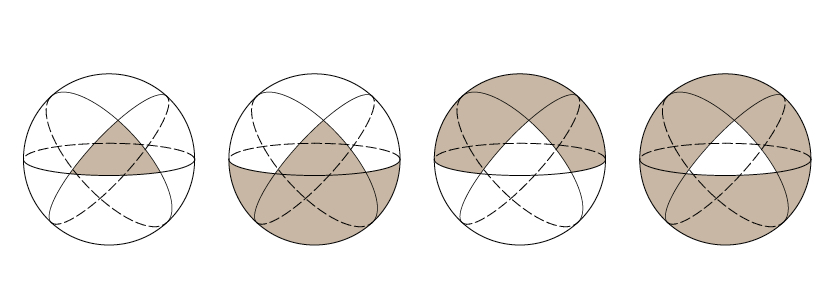
\includegraphics[width=0.9\textwidth]{kugel/Dreieckarten.jpg}
    \captionof{figure}{Dreieckarten auf einer Kugeloberfläche}
\end{center}

Der Begriff Sphärisches Dreieck oder Kugeldreieck ist ein sehr weitläufiger Begriff. 
Dabei können wir den Begriff in drei für uns wesentliche Dreiecke unterteilen:

\begin{itemize}
\item Kugelzweieck
\item Nicht Eulersche’Dreiecke
\item Eulersche’Dreiecke
\end{itemize}

\subsection{Kugelzweieck}

Zwei Grosskreise auf der Kugeloberfläche, zerlegen diese in vier gleiche Kugelzweiecke. 
Jedes dieser Dreieckseiten hat die Länge
$180^{\circ}$ oder $\pi$
Der Flächeninhalt wird dabei nur durch den Winkel $\alpha$ zwischen den beiden Grosskreisen bestimmt.

\begin{center}
        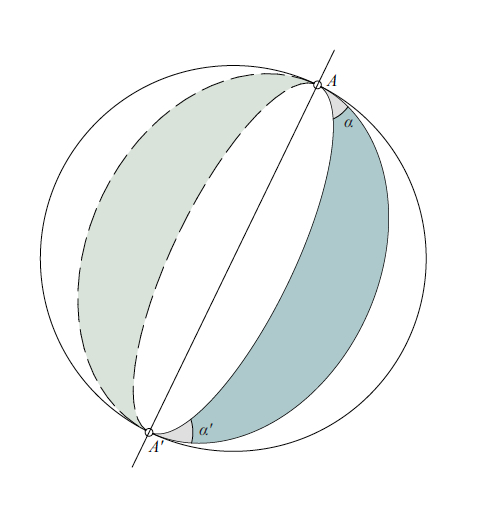
\includegraphics[width=0.3\textwidth]{kugel/Zweieck.jpg}
    \captionof{figure}{Bildung von Zweiecken durch Grosskreise}
\end{center}

Dabei ist der Flächeninhalt der ganzen Kugel:

\begin{align*}
A_{ Kugel } &= 4 \pi r^{2}
\end{align*}


Um den Flächeninhalt des betrachteten Zweieckes zu bekommen, 
müssen wir das ganze noch mit dem Kugelsegment mit dem Winkel $\alpha$ multiplizieren.

\begin{align*}
A_{ Zweieck } &= 4 \pi r^{2} \cdot \frac{ \alpha }{ 2 \pi }
\end{align*}


\subsection{Nicht Eulersche’ Dreiecke}

BLABLA

\subsection{Eulersche’ Dreiecke}

Legt man drei Grosskreise auf eine Kugeloberfläche, bilden sich dabei acht Dreiecke. 
Ein solches Dreieck heisst Eulersches’Dreieck\footnote{%
Leonard Euler (1707-1783), berühmter Schweizer Mathematiker und Physiker. 
Nicht Eulersche’Dreiecke erhält man, indem man das Äussere des Dreieckes ABC betrachtet.} 
Diese Dreiecke werden weder durch die Verlängerung ihrer Seiten durchschnitten, 
noch haben sie Dreiecksseiten welche grösser als $180^{\circ}$ sind.

\begin{center}
        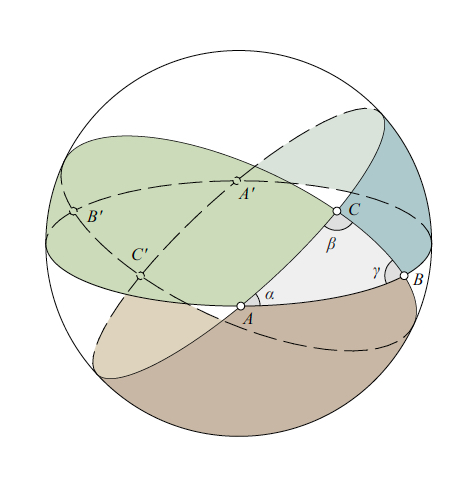
\includegraphics[width=0.4\textwidth]{kugel/Zweiecke.jpg}
    \captionof{figure}{Drei Grosskreise bilden ein sphärisches Dreieck}
\end{center}

In den nachstehenden Erklärungen und Herleitungen, sprechen wir ausschliesslich von Eulerschen’Dreiecken, da die umgeformten Winkelsätze der ebenen Trigonometrie nur auf diese Art von Kugeldreiecken angewendet werden kann.

$A_{ \overline{ ABC }}$ ist die Fläche des Dreieckes auf der Kugeloberfläche
In der ebenen Trigonometrie liegt die Winkelsumme eines Dreiecks bei
$180^{\circ}$.

Anders aber in der sphärischen Trigonometrie. Obschon sie einige Gemeinsamkeiten zur ebenen Trigonometrie aufweist, kann man nicht alles übernehmen.
So auch nicht wie Winkelsumme in einem sphärischen Dreieck.
Diese liegt bei:

\[
\begin{aligned}
\pi
&-
3\pi
&
&\text{\bigg \vert}
&
180^{\circ}
&-
540^{\circ}
\end{aligned}
\]

daraus lässt sich ableiten, das ein einzelner Winkel nicht grösser als $\pi$ oder $180^{\circ}$ sein darf. Ansonsten ist es kein Eulersches’Dreieck und wir dürfen die sphärische Trigonometrie nicht anwenden.\\
Wichtig anzumerken ist, dass die Seiten immer in Radiant beschrieben werden und nicht im Längenmass Meter wie wir es uns gewohnt sind. 
Bei den Dreiecksseiten handelt es sich um Kreisbögen und keine Strecken.

\section{Dreiecksfläche}

\begin{align*}
\text{Zweieck A}
&=
\overline{ABC} + \overline{A'BC} = 2 \alpha r^{ 2 } = A_{ \alpha }\\
\text{Zweieck B}
&=
\overline{ABC} + \overline{AB'C} = 2 \beta r^{ 2 } = A_{ \beta }\\
\text{Zweieck C}
&=
\overline{ABC} + \overline{ABC'} = 2 \gamma r^{ 2 } = A_{ \gamma }
\end{align*}

\begin{align*}
A_{ \alpha } + A_{ \beta } + A_{ \gamma } &= \frac{ 4\pi r^{ 2 } }{ 2 } + 2A_{ \overline{ ABC }} \\
2\alpha r^{ 2 } + 2\beta r^{ 2 } + 2\gamma r^{ 2 } &= \frac{ 4\pi r^{ 2 } }{ 2 } + 2A_{ \overline{ ABC }} \parallel:2\\
\alpha r^{ 2 } + \beta r^{ 2 } + \gamma r^{ 2 } &= \pi r^{ 2 } + A_{ \overline{ ABC }} \parallel-\pi r^{ 2 }\\
r^{ 2 }\left(\alpha + \beta + \gamma - \pi\right) &= A_{ \overline{ ABC }}
\end{align*}




\section{Sphärischer Exzess}
Die Winkelsumme sphärischer Dreiecke ist immer \textgreater \,  $\pi$.

\begin{align*}
\pi < \alpha + \beta + \gamma
\end{align*}

Der sphärische Exzess gibt dabei an, wie stark die Winkelsumme von $\pi$ abweicht.

\begin{align*}
\pi + \epsilon &= \alpha + \beta + \gamma \\
\epsilon &= \alpha + \beta + \gamma - \pi
\end{align*}

Würde der sphärische Exzess in der ebenen Trigonometrie angewendet, wäre dieser = 0. 
Bezieht man das auf die Erde und somit einer Kugel, kann man mit Hilfe eines beliebigen sphärischen Dreieckes und dessen Flächeninhalt auf den Radius der Kugel schliessen.

\subsection{Grenzfall - Satz von Legendre}

\begin{quote} \textit{Ein kleines sphärisches Dreieck kann näherungsweise 
wie ein ebenes Dreieck mit denselben Seiten berechnet 
werden, wenn alle Winkel des ebenen Dreiecks die um 
je ein Drittel des sphärischen Exzesses verminderten 
Winkel des sphärischen Dreiecks nimmt.} \end{quote}
\begin{flushright} - Adrien-Marie Legendre (1752-1833), Paris 1787
\end{flushright}x

Diese Aussage zeigt den Zusammenhang zwischen der 
Trigonometrie in der Ebene sowie in auf der Kugel
auf. Im speziellen bei sehr kleinen sphärischen 
Dreiecken ist die Winkelsumme nur unwesentlich 
grösser als $180^{\circ}$. Des Weiteren kann gesagt werden,
dass der sphärische Exzess gleichmässig auf alle
Winkel aufgeteilt wird.
Wichtig anzumerken ist, dass der Satz von Legendre 
für grosse, aber endliche Radien $r$ gilt.

%[SKIZZE GROSSER RADIUS/KLEINE KRÜMMUNG, KLEINER RADIUS/GROSSE KRÜMMUNG!!!!]
%


\section{Sphärisch Analoge Winkelfunktionen}

\subsection{Sphärischer Sinussatz}

Wir stellen die allgemeinen Sinussätze der Winkel $\alpha$ und $\gamma$ auf:


\[
\begin{aligned}
&{sin(\gamma)} = \frac{h}{a}
&
&\text{\bigg \vert}
&
&{sin(\alpha)} = \frac{h}{c}
&
\end{aligned}
\]

Daraus folgt:
\begin{align*}
h &= sin(\gamma)\cdot a \\
h &= sin(\alpha)\cdot c
\end{align*} 

Durch Gleichsetzung erhält man:
\begin{align*}
h &= h \\
sin(\gamma)\cdot a &= sin(\alpha)\cdot c
\end{align*} 

Durch umstellen erhalten wir den Sinussatz für a und c:
\begin{align*}
sin(\gamma)\cdot a &= sin(\alpha)\cdot c \\
\frac{sin(\gamma)}{c} &= \frac{sin(\alpha)}{a} 
\end{align*} 



\begin{align*}
\frac{sin(\alpha)}{sin(a)} = \frac{sin(\beta)}{sin(b)} = \frac{sin(\gamma)}{sin(c)}
\end{align*} 


\subsection{Winkelkosinussatz}

%[SKIZZE WINKELKOSINUS]

\[
\begin{aligned}
&\overline{C'A'} &= d\cdot {tan(b)}
&
&
&
&
&
&\overline{C'B'} &= d\cdot {tan(a)}
\end{aligned}
\]

\[
\begin{aligned}
&\overline{MA'} &= \frac{ d }{cos(b)}
&
&
&
&
&
&\overline{MB'} &= \frac{ d }{cos(a)}
\end{aligned}
\]

Der allgemeine Kosinussatz beschreibt sich wie folgt:

\begin{align*}
c^{ 2 } &= a^{ 2 } + b^{ 2 } - 2ab \cdot cos(\gamma)
\end{align*}

\begin{align*}
\triangle \overline{A'B'C' }
\overline{ A'B' }^{ 2 } &= \overline{ C'B' }^{ 2 } + \overline{ C'A' }^{ 2 } - 2 \cdot \overline{ C'B' } \cdot \overline{ C'A' } \cdot cos(\gamma)
\end{align*}



\begin{align*}
\overline{A'B'}^{ 2 } &= (d\cdot tan(a))^{ 2 } + (d\cdot tan(b))^{ 2 } - 2 \cdot (d\cdot tan(a) \cdot (d\cdot tan(b) \cdot cos(\gamma)\\
\overline{A'B'}^{ 2 } &= d^{ 2 } \cdot \left(\left(tan^{ 2 }(a) + tan^{ 2 }(b)\right) - 2\cdot tan(a) \cdot tan(b) \cdot cos(\gamma)\right)
\end{align*}

\begin{align*}
\triangle \overline{ MA'B' }
\overline{ A'B' }^{ 2 } &= \overline{ MB' }^{ 2 } + \overline{ MA' }^{ 2 } - 2\cdot \overline{ MB'} \cdot \overline{ MA' } \cdot cos(c)
\end{align*}


\begin{align*}
\overline{ A'B'}^{ 2 } &= \left(\frac{ d }{ cos(a) }  \right)^{ 2 } + \left(\frac{ d }{ cos(b)}  \right)^{ 2 } - 2 \cdot \frac{ d }{ cos(a)} \cdot \frac{ d }{ cos(b)} \cdot cos(c) \\
\overline{ A'B' }^{ 2 } &= d^{ 2 } \cdot \left(\left(\frac{ 1 }{ cos(a) }  \right)^{ 2 } + \left(\frac{ 1 }{ cos(b) }  \right)^{ 2 } - 2 \cdot \frac{ 1 }{ cos(a)} \cdot \frac{ 1 }{ cos(b)} \cdot cos(c)\right)\\
\overline{ A'B' }^{ 2 } &= d^{ 2 } \cdot \left(\left(tan^{ 2 }(a) + 1\right) + \left(tan^{ 2 }(b) + 1\right) - \left(2 \cdot \frac{cos(c)}{cos(a) \cdot cos(b)}\right)\right)
\end{align*}



\begin{align*}
\overline{ A'B'}^{ 2 } &= d^{ 2 } \cdot \left(\left(tan^{ 2 }(a) + tan^{ 2 }(b)\right) - 2 \cdot tan(a) \cdot tan(b) \cdot cos(\gamma)\right) \\
\overline{ A'B'}^{ 2 } &= d^{ 2 } \cdot \left(\left(tan^{ 2 }(a) + 1\right) + \left(tan^{ 2 }(b) + 1\right) - \left(2 \cdot \frac{cos(c)}{cos(a) \cdot cos(b)}\right)\right)
\end{align*}

Die anderen Gleichungen des Satzes, erfolgen aus Symmetriegründen.

\subsection{Seitenkosinussatz}
Durch zyklische Vertauschung des Winkelkosinus erhalten wir den Seitenkosinussatz:

\begin{align*}
{cos(a)} &= {cos(b)} \cdot {cos(c)} + {sin(b)} \cdot {sin(c)} \cdot {sin(\alpha)}\\
{cos(b)} &= {cos(a)} \cdot {cos(c)} + {sin(a)} \cdot {sin(c)} \cdot {sin(\beta)}\\
{cos(c)} &= {cos(a)} \cdot {cos(b)} + {sin(a)} \cdot {sin(b)} \cdot {sin(\gamma)}\\
\end{align*}

\section{Navigation auf See}
Das besondere an Seekarten ist die Inhaltliche Ausrichtung. Anders wie Landkarten muss sie Informationen enthalten welche für den Kapitän und seine Besatzung von grosser Bedeutung sind. Vor allem in Küstennähe ist das navigieren eines Schiffes besonders gefährlich. So enthalten Seekarten etwas über Wassertiefen, Bodenbeschaffenheiten, Gezeiten, Küstenlinien, Landzungen und Windrichtungen.
Der Hauptunterschied dabei ist, das auf der Landkarte feste Positionen definiert und aufgezeigt werden, das einzige was sich verändert ist der Reisende selbst. Bei der Seekarte ist das anders, es werden veränderliche Einwirkungen der Natur festgehalten.

Dieser kleine Unterschied zeigt die Notwendigkeit auf, die Position und den Kurs seines Schiffes auf See immer ermitteln zu können.


\section{Geographische Koordinaten}

Nachdem klar war, das die Erde eine Kugel ist, wurde diese in ein Gradnetz aufgeteilt. Dabei wurden die Angaben für eine exakte Ortsbestimmung klar definiert und die bis heute gültigen Koordinaten bestimmt.
Dabei muss man sich nochmals in Erinnerung rufen, dass sich die Erde in 24h einmal um ihre eigene Achse dreht. Nach $360 ^{\circ}$ 
und somit einer vollen Umdrehung, steht sie wieder in ihrer Ursprungsposition und ein neuer Tag beginnt.

Die Koordinaten setzen sich aus folgenden Komponenten zusammen:

\[
\begin{aligned}
&\text{Grad } (^{\circ})
&
&\text{\bigg \vert}
&
&\text{Bogenminuten } (`)
&
&\text{\bigg \vert}
&
&\text{Bogensekunden } (``)
\end{aligned}
\]

Die Erdoberfläche wurde in je 360 Breiten- und Längengrade eingeteilt. Die Breitengrade haben zueinander einen Abstand von 111.31 km, dies entspricht auch dem Abstand der Längengrade am Äquator mit Zunehmender Nähe zu den Polen, nimmt dieser Abstand ab.

\[
\begin{aligned}
&1^{\circ}
&
&\text{\bigg \vert}
&
&4 \text{ Minuten}
&
&\text{\bigg \vert}
&
&111.31\text{ km}
\end{aligned}
\]

Berechnet man nun die Erdumdrehung von 360°, erhält man genau den Erdumfang am Äquator: \begin{align*} 40’074 \text{ km.}\end{align*}

Dabei geben die Bogenminuten und -sekunden dem Standort die gewünschte Exaktheit. Mit den vollständigen Koordinaten lässt sich der Standort auf einer Landkarte exakt bestimmen und einzeichnen.

\subsection{Zeitzonen der Erde}
Wenn man nun die verschiedenen Zeitzonen der Erde betrachtet, macht die Verschiebung von jeweils einer Stunde durchaus Sinn, es lässt sich auf die Längengrade schliessen.
Zwischen den verschiedenen Zeitzonen liegen 15 Längengrade:

\begin{align*}
\text{15 Längengrade à 4 Minuten = 60 Minuten Zeitverschiebung = ca. 1665 km}
\end{align*}

Dabei ist die Zeitzone in welcher Mitte sich der Greenwich Meredian befindet die \textit{Greenwich Mean Time (GMT)} welche bis 1928 als Weltzeit galt. Im Jahr 1972 wurde diese umbenannt in die \textit{Coordinated Universal Time (UTC)} und wir von da an als Weltzeit $\pm$ 0.00 verwendet.


\section{Der Breitengrad}
Die Breitengrade bilden die bereits genannten Kleinkreise auf der Kugeloberfläche. Sie verlaufen in einem Abstand von genau 111 km parallel zum Äquator. Dabei stellt  dieser genau die Mitte zwischen Nord- und Südpol dar und teilt die Erdkugel in zwei gleiche Hälften. Somit wird von nördlicher und südlicher Breite gesprochen, je nach dem auf welcher Halbkugel man sich befindet.

%[SKIZZE DER GEOGRAFISCHEN BREITE ERDKUGEL]

\subsection{Geografische Breite $\phi$}
\begin{definition}
Die geografische Breite eines Standortes ist nichts anderes, als der Winkel am Erdmittelpunkt zwischen der Ebene des Äquators und der Geraden zum Standpunkt auf der Erdoberfläche.
\end{definition}

%[SKIZZE DER GEOGRAFISCHEN BREITE MIT WINKEL]

\subsection{Navigation mit den Breitengraden}
Da der Breitengrad bereits sehr früh ziemlich präzise bestimmt werden könnte, nutzten bereits die Seefahrer um Christoph Kolumbus den Breitengrad zur Navigation ihrer Flotten.
Den dieser lässt sich ziemlich einfach aus dem höchsten Sonnenstand oder einem Fixstern bestimmen. Dabei wird mit einem Jakobsstab\footnote{%
Der Jakobsstab ist ein früheres astronomisches Instrument zur Winkelmessung und wurde vor allem in der Seefahrt verwendet. Er ist in der Nautik der Vorläufer des Sextanten.} (später Sextant\footnote{%
Der Sextant ist ein nautisches Messinstrument zur Winkelmessung von Horizont und Fixstern (Gestirn)}) der Winkel zwischen dem Horizont und dem Fixstern gemessen. Der Winkel welchen man erhält, zieht man von 90° ab und erhält somit die geografische Breite. \\

%[SKIZZE ERMITTLUNG DES BREITENGRADES]

Wenn man sich auf der Nordhalbkugel befindet, ist der Polarstern ein sehr guter Fixstern. Befindet sich ein Schiff nun sehr nahe am Nordpol, steht dieser nahezu senkrecht am Himmelszelt bei $90^{\circ}$. Würde es aber nahe dem Äquator stehen, erscheint dieser am Horizont bei $0^{\circ}$.

\subsection{Korrekturbeiwert}

\section{Der Längengrad}
Die Längengrade bilden die bereits genannten Grosskreise auf der Kugeloberfläche.
Sie schneiden den Äquator im rechten Winkel, haben dort einen Abstand von 111 km zueinander und verbinden die Pole. Anders wie bei der geografischen Breite, ist in der Natur kein Längengrad gegeben welcher den Nullpunkt darstellt.

%[SKIZZE DER GEOGRAFISCHEN LÄNGE ERDKUGEL]

\subsection{Geografische Länge $\lambda$}
\begin{definition}
Die geografische Länge ist der Winkel an der Erdachse zum Nullmeridian.
\end{definition}

\subsection{Navigation mit den Längengraden}
Die geografische Länge lässt sich nicht so einfach bestimmen wie deren Breite. Für die Berechnung auf See benötigt man eine Referenzzeit eines Ortes mit bekannter Länge.
In der Zeit der Entdecker gab es noch keine mechanischen Uhren. Die Sonnenuhr war zudem ungeeignet, da diese nur die Uhrzeit am Standort mass und nicht die am Referenzort selbst. Die erste Pendeluhr wurde erst Mitte des 17. Jahrhunderts erfunden, was in der Schifffahrt aber auch nicht die Lösung brachte.\\
Pendeluhren auf einem Schiff sind ungeeignet, da das Pendel mit dem Wellengang aus dem Takt gebracht wird und somit die Uhr falsch geht.
Zu ungenau und gegen äussere Erschütterungen zu empfindlich waren später auch die federgetriebenen Uhren und die Unruh. Dazukamen die verschiedenen Klimazonen welche ein Schiff zu durchqueren hatten. Das Metall zog sich viel zu fest zusammen oder dehnte sich aus, was dazu führte das die Uhr unregelmässig lief.

Das sogenannte „Längenproblem“ stellte nicht nur bei der Navigation auf See ein Problem dar, es ergaben sich auch wirtschaftliche Konsequenzen. Die Schiffe mussten bis zur gewünschten geografischen Breite navigieren und segelten dann den Breitengrad entlang. Dabei waren die Schiffe oft Wochenlang unterwegs und segelten die „Breiten ab“ um an die gewünschte Position zu kommen. Dies führte zu erheblichen Zeitverlusten und viel längeren Reisezeiten.


\section{The Board of Longitude - Das Längenproblem}
Das Längenproblem beschäftigte alle grossen Seefahrernationen Europas. Wenn man bedenkt das sich Werte in einer  Höhe von halben britischen Staatshaushalten auf verloren gegangenen Schiffen befanden, erkennt man die Dringlichkeit für eine zuverlässige und genaue Navigation auf See.


\begin{itemize}
\item £ 20’000 - Abweichung von max. einem halben Grad
\item £ 15’000 - Abweichung von zwei Drittel Grad
\item £ 10’000 - Abweichung von max. $1 ^{\circ}$
\end{itemize}

\subsection{John Harrison}


\subsection{Tobias Mayer}



Uhren mit einer Abweichung von einer Minute Abweichung pro Tag (





\section{Nautische Dreieck}


$\Rightarrow$





\section{Die Vermessung der Welt}
Wir schreiben das Jahr 1818 und kehren in die Zeit des Mathematikers Carl Friedrich Gauss zurück. Neben dem liebevoll genannten „kleinen Gauss“ und anderen herausragenden Mathematischen Leistungen, beschäftigte er in den Folgejahren mit der Vermessung des Königreichs Hannovers und verfasste auf 61 Blättern das Kartenwerk \textit{Gauss’sche Landesaufnahme der 1815 durch Hannover erworbenen Gebiete}.






AUFGABE

Hubble Teleskop 
24. April 1990






\printbibliography[heading=subbibliography]
\end{refsection}




%\chapter{Geometrie auf der Kugeloberfläche\label{chapter:kugel}}
\lhead{Geometrie auf der Kugeloberfläche}
\begin{refsection}
\chapterauthor{Melina Staub und Fabian Schmid}

\section{Einleitung}

Schon seit jeher fasziniert den Menschen die Fahrt zur See. Nicht grundlos ist die Seefahrt eine der wichtigsten und ältesten Tätigkeiten der Menschheit. Der innerliche Drang neue Weltmeere und unbekannte Gebiete zu entdecken, die Fahrt zur See zu erleichtern und erträglicher zu machen, trieben die Menschen an, die Schiffe dieser Welt immer weiter zu entwickeln.

Die Idee der Kugelform der Erde ist älter als man zu denken vermag. Bereits der Schüler des antiken griechischen Philosophen Platon - Aristoteles schrieb in seiner Schrift \textit{Über den Himmel} aus dem 4. Jahrhundert v. Chr. etliche Gründe welche für die Gestallt der Erde als Kugel sprechen:

\begin{itemize}
      \item Sämtliche schweren Körper streben zum Mittelpunkt des Alls. Da sie dies von allen Seiten her gleichmäßig tun und die Erde im Mittelpunkt des Alls steht, muss sie eine kugelrunde Gestalt annehmen. 
\item Bei von der Küste wegfahrende Schiffen wird der Rumpf vor den Segeln der Sicht verborgen. 
\item In südlichen Ländern erscheinen südliche Sternbilder höher über dem Horizont.
\item Der Erdschatten bei einer Mondfinsternis ist stets rund.
\end{itemize}

Jedoch war um 1492 - der Zeit der Entdeckung Amerikas durch Christoph Kolumbus, die Idee der Erde in Kugelform noch sehr umstritten. Er erkannte anhand den Theorien und Erkenntnissen der alten Griechen, vor allem Aristoteles, das die Erde eine Kugel sein muss. \\
Doch mit seinem Vorschlag einen Seeweg über den Atlantik nach Indien zu finden und nicht wie üblich um Afrika zu segeln, stiess er beim beim portugiesischen König auf taube Ohren. Sein Plan Indien über eine Route nach Westen zu erreichen, widersprach dem gesunden Menschenverstand. Wäre die Erde wirklich eine Kugel und man befände sich auf der unteren Erdhalbkugel, würde man herunterfallen.\\
Doch auch der damals übliche Glaube an die Erde in Scheibenform brachte so einige Risiken mit sich. Was würde passieren, wenn die Flotte das Ende der Scheibe erreicht hatte? Würden sie über den Erdrand hinweggleiten und in den Abgrund stürzen?\\
Erst nach viel Überzeugungsarbeit durch Kolumbus, setzte er sich am Spanischen Hof durch und segelte über die Westliche Route über den Atlantik und entdeckte schlussendlich Amerika.

Der praktische und greifbare Beweis das die Erde eine Kugel ist, lieferte rund 30 Jahre später der Portugiese Fernando Magellan. Mit seiner Weltumsegelung und seiner Ankunft in den Philippinen, bewies er definitiv das die Erde eine Kugel ist.\\

Nun wollen wir uns die Frage stellen, wie die alten Seefahrer ohne GPS und jeglichen modernen Navigationssystemen auf hoher See wussten wo sie sich befinden und was haben die Sterne mit alldem zu tun? Reisen Sie mit uns zurück in eine Zeit mit Sextant, Kompass und Sternkarten. In die Zeit der Seefahrer und Entdecker.


\section{Geometrie auf der Ebene und der Kugel}

Euklid von Alexandria beschrieb die Grundbegriffe der ebenen Geometrie mittels Punkt, Geraden, Ebene, Winkel und Dreieck. Diese Dreiecke lassen sich mithilfe der ebenen Trigonometrie beschreiben. Dabei gelten die uns bekannten trigonometrischen Winkelfunktionen:\\

\text{Sinussatz:}
\begin{align*}
\frac{ a }{ sin(\alpha) } &= \frac{ b }{sin(\beta)} = \frac{ c }{ sin(\gamma) } = \frac{abc}{2A} = 2r\\
\end{align*}

\text{Cosinussatz:}
\begin{align*}
c^{ 2 } &= a^{ 2 } + b^{ 2 } - 2ab\cdot cos(\gamma)\\
b^{ 2 } &= a^{ 2 } + c^{ 2 } - 2ab\cdot cos(\beta)\\
a^{ 2 } &= b^{ 2 } + c^{ 2 } - 2ab\cdot cos(\alpha)
\end{align*}

Um Dreiecke auf der Kugeloberfläche zu berechnen, benötigt man die sphärische Trigonometrie. Die oben beschriebenen Sätze lassen sich auf der Kugel nicht anwenden, sie werden aber als Grundlage zur Herleitung der Sätze für das Kugeldreieck benötigt.

Die nachfolgenden Seiten thematisieren die Geometrie auf der Kugeloberfläche und wie sie in der Navigation eingesetzt werden kann.


\section{Gross- und Kleinkreise}

Eine Kugeloberfläche lässt sich in zwei verschiedene Kreisarten einteilen -  Gross- und Kleinkreise. 
Wir betrachten als erstes die Grosskreise:

\begin{definition}
Ein Großkreis ist ein größtmöglicher Kreis auf einer Kugeloberfläche. Sein Mittelpunkt fällt immer mit dem Mittelpunkt der Kugel zusammen und ein Schnitt auf dem Großkreis teilt die Kugel in jedem Fall in zwei („gleich große“) Hälften.
\end{definition}

Es gibt unendlich viele Möglichkeiten, eine Kugel in zwei gleich grosse Stücke zu zerschneiden, 
daher gibt es auch unendlich viele Grosskreise. Wenn wir die Grosskreise auf einer Kugel mit diesen auf der Erde beschreiben, sprechen wir von den Längengraden aber auch der Äquator beschreibt einen Grosskreis.
Ein Elementarer Bestandteil bilden die Grosskreise in der sphärischen Trigonometrie. Mithilfe der Schnittpunkte verschiedener Grosskreise, lässt sich ein Sphärisches Dreieck bilden auf welchem sich die sphärische Trigonometrie anwenden lässt.

[GRAFIK GROSSKREISE]

\begin{definition}
Unter Kleinkreis versteht man jene Kreise auf einer Kugeloberfläche, deren Ebenen nicht den Kugelmittelpunkt enthalten.
\end{definition}

Die Kleinkreise eignen sich im Gegensatz zu den Grosskreisen \textit{nicht} für die sphärische Trigonometrie. 
Sie werden lediglich zur Bestimmung der Messgrössen, Winkelabstände oder des Höhenwinkels eines Gestirns verwendet. 

Wenn wir die Kleinkreise auf die Erdoberfläche projizieren betrachten wir die Breitengrade.

[GRAFIK KLEINKREISE]


\section{Sphärische Dreiecke / Kugeldreieck}

\begin{center}
        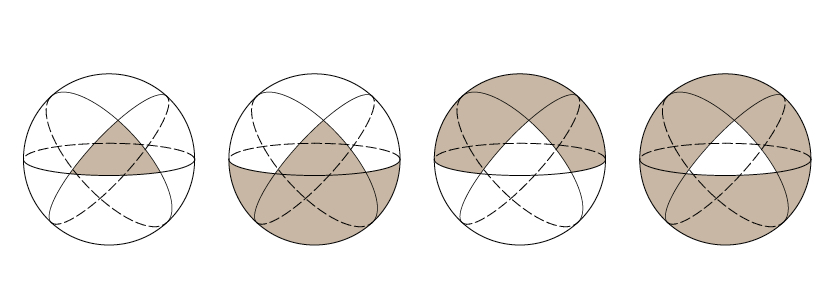
\includegraphics[width=0.9\textwidth]{kugel/Dreieckarten.jpg}
    \captionof{figure}{Dreieckarten auf einer Kugeloberfläche}
\end{center}

Der Begriff Sphärisches Dreieck oder Kugeldreieck ist ein sehr weitläufiger Begriff. 
Dabei können wir den Begriff in drei für uns wesentliche Dreiecke unterteilen:

\begin{itemize}
\item Kugelzweieck
\item Nicht Eulersche’Dreiecke
\item Eulersche’Dreiecke
\end{itemize}

\subsection{Kugelzweieck}

Zwei Grosskreise auf der Kugeloberfläche, zerlegen diese in vier gleiche Kugelzweiecke. 
Jedes dieser Dreieckseiten hat die Länge
$180^{\circ}$ oder $\pi$
Der Flächeninhalt wird dabei nur durch den Winkel $\alpha$ zwischen den beiden Grosskreisen bestimmt.

\begin{center}
        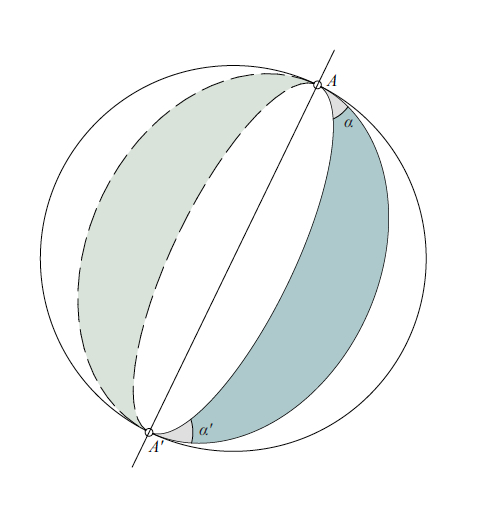
\includegraphics[width=0.3\textwidth]{kugel/Zweieck.jpg}
    \captionof{figure}{Bildung von Zweiecken durch Grosskreise}
\end{center}

Dabei ist der Flächeninhalt der ganzen Kugel:

\begin{align*}
A_{ Kugel } &= 4 \pi r^{2}
\end{align*}


Um den Flächeninhalt des betrachteten Zweieckes zu bekommen, 
müssen wir das ganze noch mit dem Kugelsegment mit dem Winkel $\alpha$ multiplizieren.

\begin{align*}
A_{ Zweieck } &= 4 \pi r^{2} \cdot \frac{ \alpha }{ 2 \pi }
\end{align*}


\subsection{Nicht Eulersche’ Dreiecke}

BLABLA

\subsection{Eulersche’ Dreiecke}

Legt man drei Grosskreise auf eine Kugeloberfläche, bilden sich dabei acht Dreiecke. 
Ein solches Dreieck heisst Eulersches’Dreieck\footnote{%
Leonard Euler (1707-1783), berühmter Schweizer Mathematiker und Physiker. 
Nicht Eulersche’Dreiecke erhält man, indem man das Äussere des Dreieckes ABC betrachtet.} 
Diese Dreiecke werden weder durch die Verlängerung ihrer Seiten durchschnitten, 
noch haben sie Dreiecksseiten welche grösser als $180^{\circ}$ sind.

\begin{center}
        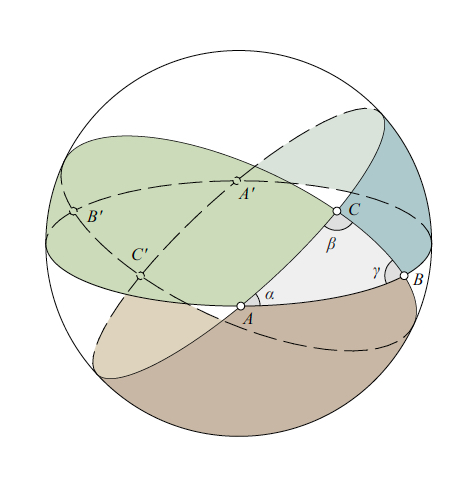
\includegraphics[width=0.4\textwidth]{kugel/Zweiecke.jpg}
    \captionof{figure}{Drei Grosskreise bilden ein sphärisches Dreieck}
\end{center}

In den nachstehenden Erklärungen und Herleitungen, sprechen wir ausschliesslich von Eulerschen’Dreiecken, da die umgeformten Winkelsätze der ebenen Trigonometrie nur auf diese Art von Kugeldreiecken angewendet werden kann.

$A_{ \overline{ ABC }}$ ist die Fläche des Dreieckes auf der Kugeloberfläche
In der ebenen Trigonometrie liegt die Winkelsumme eines Dreiecks bei
$180^{\circ}$.

Anders aber in der sphärischen Trigonometrie. Obschon sie einige Gemeinsamkeiten zur ebenen Trigonometrie aufweist, kann man nicht alles übernehmen.
So auch nicht wie Winkelsumme in einem sphärischen Dreieck.
Diese liegt bei:

\[
\begin{aligned}
\pi
&-
3\pi
&
&\text{\bigg \vert}
&
180^{\circ}
&-
540^{\circ}
\end{aligned}
\]

daraus lässt sich ableiten, das ein einzelner Winkel nicht grösser als $\pi$ oder $180^{\circ}$ sein darf. Ansonsten ist es kein Eulersches’Dreieck und wir dürfen die sphärische Trigonometrie nicht anwenden.\\
Wichtig anzumerken ist, dass die Seiten immer in Radiant beschrieben werden und nicht im Längenmass Meter wie wir es uns gewohnt sind. 
Bei den Dreiecksseiten handelt es sich um Kreisbögen und keine Strecken.

\section{Dreiecksfläche}

\begin{align*}
\text{Zweieck A}
&=
\overline{ABC} + \overline{A'BC} = 2 \alpha r^{ 2 } = A_{ \alpha }\\
\text{Zweieck B}
&=
\overline{ABC} + \overline{AB'C} = 2 \beta r^{ 2 } = A_{ \beta }\\
\text{Zweieck C}
&=
\overline{ABC} + \overline{ABC'} = 2 \gamma r^{ 2 } = A_{ \gamma }
\end{align*}

\begin{align*}
A_{ \alpha } + A_{ \beta } + A_{ \gamma } &= \frac{ 4\pi r^{ 2 } }{ 2 } + 2A_{ \overline{ ABC }} \\
2\alpha r^{ 2 } + 2\beta r^{ 2 } + 2\gamma r^{ 2 } &= \frac{ 4\pi r^{ 2 } }{ 2 } + 2A_{ \overline{ ABC }} \parallel:2\\
\alpha r^{ 2 } + \beta r^{ 2 } + \gamma r^{ 2 } &= \pi r^{ 2 } + A_{ \overline{ ABC }} \parallel-\pi r^{ 2 }\\
r^{ 2 }\left(\alpha + \beta + \gamma - \pi\right) &= A_{ \overline{ ABC }}
\end{align*}




\section{Sphärischer Exzess}
Die Winkelsumme sphärischer Dreiecke ist immer \textgreater \,  $\pi$.

\begin{align*}
\pi < \alpha + \beta + \gamma
\end{align*}

Der sphärische Exzess gibt dabei an, wie stark die Winkelsumme von $\pi$ abweicht.

\begin{align*}
\pi + \epsilon &= \alpha + \beta + \gamma \\
\epsilon &= \alpha + \beta + \gamma - \pi
\end{align*}

Würde der sphärische Exzess in der ebenen Trigonometrie angewendet, wäre dieser = 0. 
Bezieht man das auf die Erde und somit einer Kugel, kann man mit Hilfe eines beliebigen sphärischen Dreieckes und dessen Flächeninhalt auf den Radius der Kugel schliessen.

\subsection{Grenzfall - Satz von Legendre}

\begin{quote} \textit{Ein kleines sphärisches Dreieck kann näherungsweise 
wie ein ebenes Dreieck mit denselben Seiten berechnet 
werden, wenn alle Winkel des ebenen Dreiecks die um 
je ein Drittel des sphärischen Exzesses verminderten 
Winkel des sphärischen Dreiecks nimmt.} \end{quote}
\begin{flushright} - Adrien-Marie Legendre (1752-1833), Paris 1787
\end{flushright}x

Diese Aussage zeigt den Zusammenhang zwischen der 
Trigonometrie in der Ebene sowie in auf der Kugel
auf. Im speziellen bei sehr kleinen sphärischen 
Dreiecken ist die Winkelsumme nur unwesentlich 
grösser als $180^{\circ}$. Des Weiteren kann gesagt werden,
dass der sphärische Exzess gleichmässig auf alle
Winkel aufgeteilt wird.
Wichtig anzumerken ist, dass der Satz von Legendre 
für grosse, aber endliche Radien $r$ gilt.

%[SKIZZE GROSSER RADIUS/KLEINE KRÜMMUNG, KLEINER RADIUS/GROSSE KRÜMMUNG!!!!]
%


\section{Sphärisch Analoge Winkelfunktionen}

\subsection{Sphärischer Sinussatz}

Wir stellen die allgemeinen Sinussätze der Winkel $\alpha$ und $\gamma$ auf:


\[
\begin{aligned}
&{sin(\gamma)} = \frac{h}{a}
&
&\text{\bigg \vert}
&
&{sin(\alpha)} = \frac{h}{c}
&
\end{aligned}
\]

Daraus folgt:
\begin{align*}
h &= sin(\gamma)\cdot a \\
h &= sin(\alpha)\cdot c
\end{align*} 

Durch Gleichsetzung erhält man:
\begin{align*}
h &= h \\
sin(\gamma)\cdot a &= sin(\alpha)\cdot c
\end{align*} 

Durch umstellen erhalten wir den Sinussatz für a und c:
\begin{align*}
sin(\gamma)\cdot a &= sin(\alpha)\cdot c \\
\frac{sin(\gamma)}{c} &= \frac{sin(\alpha)}{a} 
\end{align*} 



\begin{align*}
\frac{sin(\alpha)}{sin(a)} = \frac{sin(\beta)}{sin(b)} = \frac{sin(\gamma)}{sin(c)}
\end{align*} 


\subsection{Winkelkosinussatz}

%[SKIZZE WINKELKOSINUS]

\[
\begin{aligned}
&\overline{C'A'} &= d\cdot {tan(b)}
&
&
&
&
&
&\overline{C'B'} &= d\cdot {tan(a)}
\end{aligned}
\]

\[
\begin{aligned}
&\overline{MA'} &= \frac{ d }{cos(b)}
&
&
&
&
&
&\overline{MB'} &= \frac{ d }{cos(a)}
\end{aligned}
\]

Der allgemeine Kosinussatz beschreibt sich wie folgt:

\begin{align*}
c^{ 2 } &= a^{ 2 } + b^{ 2 } - 2ab \cdot cos(\gamma)
\end{align*}

\begin{align*}
\triangle \overline{A'B'C' }
\overline{ A'B' }^{ 2 } &= \overline{ C'B' }^{ 2 } + \overline{ C'A' }^{ 2 } - 2 \cdot \overline{ C'B' } \cdot \overline{ C'A' } \cdot cos(\gamma)
\end{align*}



\begin{align*}
\overline{A'B'}^{ 2 } &= (d\cdot tan(a))^{ 2 } + (d\cdot tan(b))^{ 2 } - 2 \cdot (d\cdot tan(a) \cdot (d\cdot tan(b) \cdot cos(\gamma)\\
\overline{A'B'}^{ 2 } &= d^{ 2 } \cdot \left(\left(tan^{ 2 }(a) + tan^{ 2 }(b)\right) - 2\cdot tan(a) \cdot tan(b) \cdot cos(\gamma)\right)
\end{align*}

\begin{align*}
\triangle \overline{ MA'B' }
\overline{ A'B' }^{ 2 } &= \overline{ MB' }^{ 2 } + \overline{ MA' }^{ 2 } - 2\cdot \overline{ MB'} \cdot \overline{ MA' } \cdot cos(c)
\end{align*}


\begin{align*}
\overline{ A'B'}^{ 2 } &= \left(\frac{ d }{ cos(a) }  \right)^{ 2 } + \left(\frac{ d }{ cos(b)}  \right)^{ 2 } - 2 \cdot \frac{ d }{ cos(a)} \cdot \frac{ d }{ cos(b)} \cdot cos(c) \\
\overline{ A'B' }^{ 2 } &= d^{ 2 } \cdot \left(\left(\frac{ 1 }{ cos(a) }  \right)^{ 2 } + \left(\frac{ 1 }{ cos(b) }  \right)^{ 2 } - 2 \cdot \frac{ 1 }{ cos(a)} \cdot \frac{ 1 }{ cos(b)} \cdot cos(c)\right)\\
\overline{ A'B' }^{ 2 } &= d^{ 2 } \cdot \left(\left(tan^{ 2 }(a) + 1\right) + \left(tan^{ 2 }(b) + 1\right) - \left(2 \cdot \frac{cos(c)}{cos(a) \cdot cos(b)}\right)\right)
\end{align*}



\begin{align*}
\overline{ A'B'}^{ 2 } &= d^{ 2 } \cdot \left(\left(tan^{ 2 }(a) + tan^{ 2 }(b)\right) - 2 \cdot tan(a) \cdot tan(b) \cdot cos(\gamma)\right) \\
\overline{ A'B'}^{ 2 } &= d^{ 2 } \cdot \left(\left(tan^{ 2 }(a) + 1\right) + \left(tan^{ 2 }(b) + 1\right) - \left(2 \cdot \frac{cos(c)}{cos(a) \cdot cos(b)}\right)\right)
\end{align*}

Die anderen Gleichungen des Satzes, erfolgen aus Symmetriegründen.

\subsection{Seitenkosinussatz}
Durch zyklische Vertauschung des Winkelkosinus erhalten wir den Seitenkosinussatz:

\begin{align*}
{cos(a)} &= {cos(b)} \cdot {cos(c)} + {sin(b)} \cdot {sin(c)} \cdot {sin(\alpha)}\\
{cos(b)} &= {cos(a)} \cdot {cos(c)} + {sin(a)} \cdot {sin(c)} \cdot {sin(\beta)}\\
{cos(c)} &= {cos(a)} \cdot {cos(b)} + {sin(a)} \cdot {sin(b)} \cdot {sin(\gamma)}\\
\end{align*}

\section{Navigation auf See}
Das besondere an Seekarten ist die Inhaltliche Ausrichtung. Anders wie Landkarten muss sie Informationen enthalten welche für den Kapitän und seine Besatzung von grosser Bedeutung sind. Vor allem in Küstennähe ist das navigieren eines Schiffes besonders gefährlich. So enthalten Seekarten etwas über Wassertiefen, Bodenbeschaffenheiten, Gezeiten, Küstenlinien, Landzungen und Windrichtungen.
Der Hauptunterschied dabei ist, das auf der Landkarte feste Positionen definiert und aufgezeigt werden, das einzige was sich verändert ist der Reisende selbst. Bei der Seekarte ist das anders, es werden veränderliche Einwirkungen der Natur festgehalten.

Dieser kleine Unterschied zeigt die Notwendigkeit auf, die Position und den Kurs seines Schiffes auf See immer ermitteln zu können.


\section{Geographische Koordinaten}

Nachdem klar war, das die Erde eine Kugel ist, wurde diese in ein Gradnetz aufgeteilt. Dabei wurden die Angaben für eine exakte Ortsbestimmung klar definiert und die bis heute gültigen Koordinaten bestimmt.
Dabei muss man sich nochmals in Erinnerung rufen, dass sich die Erde in 24h einmal um ihre eigene Achse dreht. Nach $360 ^{\circ}$ 
und somit einer vollen Umdrehung, steht sie wieder in ihrer Ursprungsposition und ein neuer Tag beginnt.

Die Koordinaten setzen sich aus folgenden Komponenten zusammen:

\[
\begin{aligned}
&\text{Grad } (^{\circ})
&
&\text{\bigg \vert}
&
&\text{Bogenminuten } (`)
&
&\text{\bigg \vert}
&
&\text{Bogensekunden } (``)
\end{aligned}
\]

Die Erdoberfläche wurde in je 360 Breiten- und Längengrade eingeteilt. Die Breitengrade haben zueinander einen Abstand von 111.31 km, dies entspricht auch dem Abstand der Längengrade am Äquator mit Zunehmender Nähe zu den Polen, nimmt dieser Abstand ab.

\[
\begin{aligned}
&1^{\circ}
&
&\text{\bigg \vert}
&
&4 \text{ Minuten}
&
&\text{\bigg \vert}
&
&111.31\text{ km}
\end{aligned}
\]

Berechnet man nun die Erdumdrehung von 360°, erhält man genau den Erdumfang am Äquator: \begin{align*} 40’074 \text{ km.}\end{align*}

Dabei geben die Bogenminuten und -sekunden dem Standort die gewünschte Exaktheit. Mit den vollständigen Koordinaten lässt sich der Standort auf einer Landkarte exakt bestimmen und einzeichnen.

\subsection{Zeitzonen der Erde}
Wenn man nun die verschiedenen Zeitzonen der Erde betrachtet, macht die Verschiebung von jeweils einer Stunde durchaus Sinn, es lässt sich auf die Längengrade schliessen.
Zwischen den verschiedenen Zeitzonen liegen 15 Längengrade:

\begin{align*}
\text{15 Längengrade à 4 Minuten = 60 Minuten Zeitverschiebung = ca. 1665 km}
\end{align*}

Dabei ist die Zeitzone in welcher Mitte sich der Greenwich Meredian befindet die \textit{Greenwich Mean Time (GMT)} welche bis 1928 als Weltzeit galt. Im Jahr 1972 wurde diese umbenannt in die \textit{Coordinated Universal Time (UTC)} und wir von da an als Weltzeit $\pm$ 0.00 verwendet.


\section{Der Breitengrad}
Die Breitengrade bilden die bereits genannten Kleinkreise auf der Kugeloberfläche. Sie verlaufen in einem Abstand von genau 111 km parallel zum Äquator. Dabei stellt  dieser genau die Mitte zwischen Nord- und Südpol dar und teilt die Erdkugel in zwei gleiche Hälften. Somit wird von nördlicher und südlicher Breite gesprochen, je nach dem auf welcher Halbkugel man sich befindet.

%[SKIZZE DER GEOGRAFISCHEN BREITE ERDKUGEL]

\subsection{Geografische Breite $\phi$}
\begin{definition}
Die geografische Breite eines Standortes ist nichts anderes, als der Winkel am Erdmittelpunkt zwischen der Ebene des Äquators und der Geraden zum Standpunkt auf der Erdoberfläche.
\end{definition}

%[SKIZZE DER GEOGRAFISCHEN BREITE MIT WINKEL]

\subsection{Navigation mit den Breitengraden}
Da der Breitengrad bereits sehr früh ziemlich präzise bestimmt werden könnte, nutzten bereits die Seefahrer um Christoph Kolumbus den Breitengrad zur Navigation ihrer Flotten.
Den dieser lässt sich ziemlich einfach aus dem höchsten Sonnenstand oder einem Fixstern bestimmen. Dabei wird mit einem Jakobsstab\footnote{%
Der Jakobsstab ist ein früheres astronomisches Instrument zur Winkelmessung und wurde vor allem in der Seefahrt verwendet. Er ist in der Nautik der Vorläufer des Sextanten.} (später Sextant\footnote{%
Der Sextant ist ein nautisches Messinstrument zur Winkelmessung von Horizont und Fixstern (Gestirn)}) der Winkel zwischen dem Horizont und dem Fixstern gemessen. Der Winkel welchen man erhält, zieht man von 90° ab und erhält somit die geografische Breite. \\

%[SKIZZE ERMITTLUNG DES BREITENGRADES]

Wenn man sich auf der Nordhalbkugel befindet, ist der Polarstern ein sehr guter Fixstern. Befindet sich ein Schiff nun sehr nahe am Nordpol, steht dieser nahezu senkrecht am Himmelszelt bei $90^{\circ}$. Würde es aber nahe dem Äquator stehen, erscheint dieser am Horizont bei $0^{\circ}$.

\subsection{Korrekturbeiwert}

\section{Der Längengrad}
Die Längengrade bilden die bereits genannten Grosskreise auf der Kugeloberfläche.
Sie schneiden den Äquator im rechten Winkel, haben dort einen Abstand von 111 km zueinander und verbinden die Pole. Anders wie bei der geografischen Breite, ist in der Natur kein Längengrad gegeben welcher den Nullpunkt darstellt.

%[SKIZZE DER GEOGRAFISCHEN LÄNGE ERDKUGEL]

\subsection{Geografische Länge $\lambda$}
\begin{definition}
Die geografische Länge ist der Winkel an der Erdachse zum Nullmeridian.
\end{definition}

\subsection{Navigation mit den Längengraden}
Die geografische Länge lässt sich nicht so einfach bestimmen wie deren Breite. Für die Berechnung auf See benötigt man eine Referenzzeit eines Ortes mit bekannter Länge.
In der Zeit der Entdecker gab es noch keine mechanischen Uhren. Die Sonnenuhr war zudem ungeeignet, da diese nur die Uhrzeit am Standort mass und nicht die am Referenzort selbst. Die erste Pendeluhr wurde erst Mitte des 17. Jahrhunderts erfunden, was in der Schifffahrt aber auch nicht die Lösung brachte.\\
Pendeluhren auf einem Schiff sind ungeeignet, da das Pendel mit dem Wellengang aus dem Takt gebracht wird und somit die Uhr falsch geht.
Zu ungenau und gegen äussere Erschütterungen zu empfindlich waren später auch die federgetriebenen Uhren und die Unruh. Dazukamen die verschiedenen Klimazonen welche ein Schiff zu durchqueren hatten. Das Metall zog sich viel zu fest zusammen oder dehnte sich aus, was dazu führte das die Uhr unregelmässig lief.

Das sogenannte „Längenproblem“ stellte nicht nur bei der Navigation auf See ein Problem dar, es ergaben sich auch wirtschaftliche Konsequenzen. Die Schiffe mussten bis zur gewünschten geografischen Breite navigieren und segelten dann den Breitengrad entlang. Dabei waren die Schiffe oft Wochenlang unterwegs und segelten die „Breiten ab“ um an die gewünschte Position zu kommen. Dies führte zu erheblichen Zeitverlusten und viel längeren Reisezeiten.


\section{The Board of Longitude - Das Längenproblem}
Das Längenproblem beschäftigte alle grossen Seefahrernationen Europas. Wenn man bedenkt das sich Werte in einer  Höhe von halben britischen Staatshaushalten auf verloren gegangenen Schiffen befanden, erkennt man die Dringlichkeit für eine zuverlässige und genaue Navigation auf See.


\begin{itemize}
\item £ 20’000 - Abweichung von max. einem halben Grad
\item £ 15’000 - Abweichung von zwei Drittel Grad
\item £ 10’000 - Abweichung von max. $1 ^{\circ}$
\end{itemize}

\subsection{John Harrison}


\subsection{Tobias Mayer}



Uhren mit einer Abweichung von einer Minute Abweichung pro Tag (





\section{Nautische Dreieck}


$\Rightarrow$





\section{Die Vermessung der Welt}
Wir schreiben das Jahr 1818 und kehren in die Zeit des Mathematikers Carl Friedrich Gauss zurück. Neben dem liebevoll genannten „kleinen Gauss“ und anderen herausragenden Mathematischen Leistungen, beschäftigte er in den Folgejahren mit der Vermessung des Königreichs Hannovers und verfasste auf 61 Blättern das Kartenwerk \textit{Gauss’sche Landesaufnahme der 1815 durch Hannover erworbenen Gebiete}.






AUFGABE

Hubble Teleskop 
24. April 1990






\printbibliography[heading=subbibliography]
\end{refsection}




%\chapter{Geometrie auf der Kugeloberfläche\label{chapter:kugel}}
\lhead{Geometrie auf der Kugeloberfläche}
\begin{refsection}
\chapterauthor{Melina Staub und Fabian Schmid}

\section{Einleitung}

Schon seit jeher fasziniert den Menschen die Fahrt zur See. Nicht grundlos ist die Seefahrt eine der wichtigsten und ältesten Tätigkeiten der Menschheit. Der innerliche Drang neue Weltmeere und unbekannte Gebiete zu entdecken, die Fahrt zur See zu erleichtern und erträglicher zu machen, trieben die Menschen an, die Schiffe dieser Welt immer weiter zu entwickeln.

Die Idee der Kugelform der Erde ist älter als man zu denken vermag. Bereits der Schüler des antiken griechischen Philosophen Platon - Aristoteles schrieb in seiner Schrift \textit{Über den Himmel} aus dem 4. Jahrhundert v. Chr. etliche Gründe welche für die Gestallt der Erde als Kugel sprechen:

\begin{itemize}
      \item Sämtliche schweren Körper streben zum Mittelpunkt des Alls. Da sie dies von allen Seiten her gleichmäßig tun und die Erde im Mittelpunkt des Alls steht, muss sie eine kugelrunde Gestalt annehmen. 
\item Bei von der Küste wegfahrende Schiffen wird der Rumpf vor den Segeln der Sicht verborgen. 
\item In südlichen Ländern erscheinen südliche Sternbilder höher über dem Horizont.
\item Der Erdschatten bei einer Mondfinsternis ist stets rund.
\end{itemize}

Jedoch war um 1492 - der Zeit der Entdeckung Amerikas durch Christoph Kolumbus, die Idee der Erde in Kugelform noch sehr umstritten. Er erkannte anhand den Theorien und Erkenntnissen der alten Griechen, vor allem Aristoteles, das die Erde eine Kugel sein muss. \\
Doch mit seinem Vorschlag einen Seeweg über den Atlantik nach Indien zu finden und nicht wie üblich um Afrika zu segeln, stiess er beim beim portugiesischen König auf taube Ohren. Sein Plan Indien über eine Route nach Westen zu erreichen, widersprach dem gesunden Menschenverstand. Wäre die Erde wirklich eine Kugel und man befände sich auf der unteren Erdhalbkugel, würde man herunterfallen.\\
Doch auch der damals übliche Glaube an die Erde in Scheibenform brachte so einige Risiken mit sich. Was würde passieren, wenn die Flotte das Ende der Scheibe erreicht hatte? Würden sie über den Erdrand hinweggleiten und in den Abgrund stürzen?\\
Erst nach viel Überzeugungsarbeit durch Kolumbus, setzte er sich am Spanischen Hof durch und segelte über die Westliche Route über den Atlantik und entdeckte schlussendlich Amerika.

Der praktische und greifbare Beweis das die Erde eine Kugel ist, lieferte rund 30 Jahre später der Portugiese Fernando Magellan. Mit seiner Weltumsegelung und seiner Ankunft in den Philippinen, bewies er definitiv das die Erde eine Kugel ist.\\

Nun wollen wir uns die Frage stellen, wie die alten Seefahrer ohne GPS und jeglichen modernen Navigationssystemen auf hoher See wussten wo sie sich befinden und was haben die Sterne mit alldem zu tun? Reisen Sie mit uns zurück in eine Zeit mit Sextant, Kompass und Sternkarten. In die Zeit der Seefahrer und Entdecker.


\section{Geometrie auf der Ebene und der Kugel}

Euklid von Alexandria beschrieb die Grundbegriffe der ebenen Geometrie mittels Punkt, Geraden, Ebene, Winkel und Dreieck. Diese Dreiecke lassen sich mithilfe der ebenen Trigonometrie beschreiben. Dabei gelten die uns bekannten trigonometrischen Winkelfunktionen:\\

\text{Sinussatz:}
\begin{align*}
\frac{ a }{ sin(\alpha) } &= \frac{ b }{sin(\beta)} = \frac{ c }{ sin(\gamma) } = \frac{abc}{2A} = 2r\\
\end{align*}

\text{Cosinussatz:}
\begin{align*}
c^{ 2 } &= a^{ 2 } + b^{ 2 } - 2ab\cdot cos(\gamma)\\
b^{ 2 } &= a^{ 2 } + c^{ 2 } - 2ab\cdot cos(\beta)\\
a^{ 2 } &= b^{ 2 } + c^{ 2 } - 2ab\cdot cos(\alpha)
\end{align*}

Um Dreiecke auf der Kugeloberfläche zu berechnen, benötigt man die sphärische Trigonometrie. Die oben beschriebenen Sätze lassen sich auf der Kugel nicht anwenden, sie werden aber als Grundlage zur Herleitung der Sätze für das Kugeldreieck benötigt.

Die nachfolgenden Seiten thematisieren die Geometrie auf der Kugeloberfläche und wie sie in der Navigation eingesetzt werden kann.


\section{Gross- und Kleinkreise}

Eine Kugeloberfläche lässt sich in zwei verschiedene Kreisarten einteilen -  Gross- und Kleinkreise. 
Wir betrachten als erstes die Grosskreise:

\begin{definition}
Ein Großkreis ist ein größtmöglicher Kreis auf einer Kugeloberfläche. Sein Mittelpunkt fällt immer mit dem Mittelpunkt der Kugel zusammen und ein Schnitt auf dem Großkreis teilt die Kugel in jedem Fall in zwei („gleich große“) Hälften.
\end{definition}

Es gibt unendlich viele Möglichkeiten, eine Kugel in zwei gleich grosse Stücke zu zerschneiden, 
daher gibt es auch unendlich viele Grosskreise. Wenn wir die Grosskreise auf einer Kugel mit diesen auf der Erde beschreiben, sprechen wir von den Längengraden aber auch der Äquator beschreibt einen Grosskreis.
Ein Elementarer Bestandteil bilden die Grosskreise in der sphärischen Trigonometrie. Mithilfe der Schnittpunkte verschiedener Grosskreise, lässt sich ein Sphärisches Dreieck bilden auf welchem sich die sphärische Trigonometrie anwenden lässt.

[GRAFIK GROSSKREISE]

\begin{definition}
Unter Kleinkreis versteht man jene Kreise auf einer Kugeloberfläche, deren Ebenen nicht den Kugelmittelpunkt enthalten.
\end{definition}

Die Kleinkreise eignen sich im Gegensatz zu den Grosskreisen \textit{nicht} für die sphärische Trigonometrie. 
Sie werden lediglich zur Bestimmung der Messgrössen, Winkelabstände oder des Höhenwinkels eines Gestirns verwendet. 

Wenn wir die Kleinkreise auf die Erdoberfläche projizieren betrachten wir die Breitengrade.

[GRAFIK KLEINKREISE]


\section{Sphärische Dreiecke / Kugeldreieck}

\begin{center}
        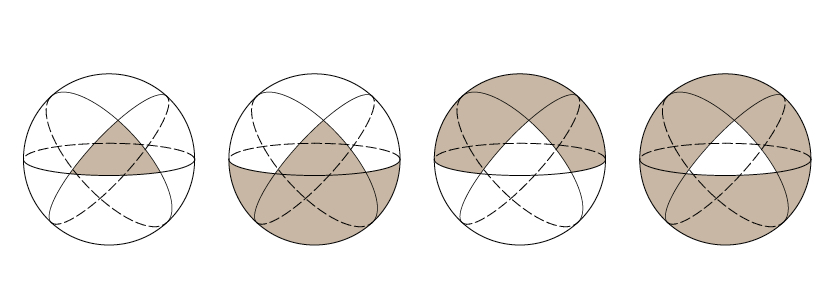
\includegraphics[width=0.9\textwidth]{kugel/Dreieckarten.jpg}
    \captionof{figure}{Dreieckarten auf einer Kugeloberfläche}
\end{center}

Der Begriff Sphärisches Dreieck oder Kugeldreieck ist ein sehr weitläufiger Begriff. 
Dabei können wir den Begriff in drei für uns wesentliche Dreiecke unterteilen:

\begin{itemize}
\item Kugelzweieck
\item Nicht Eulersche’Dreiecke
\item Eulersche’Dreiecke
\end{itemize}

\subsection{Kugelzweieck}

Zwei Grosskreise auf der Kugeloberfläche, zerlegen diese in vier gleiche Kugelzweiecke. 
Jedes dieser Dreieckseiten hat die Länge
$180^{\circ}$ oder $\pi$
Der Flächeninhalt wird dabei nur durch den Winkel $\alpha$ zwischen den beiden Grosskreisen bestimmt.

\begin{center}
        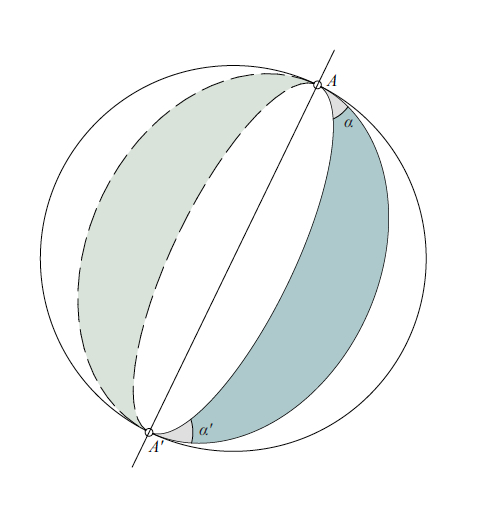
\includegraphics[width=0.3\textwidth]{kugel/Zweieck.jpg}
    \captionof{figure}{Bildung von Zweiecken durch Grosskreise}
\end{center}

Dabei ist der Flächeninhalt der ganzen Kugel:

\begin{align*}
A_{ Kugel } &= 4 \pi r^{2}
\end{align*}


Um den Flächeninhalt des betrachteten Zweieckes zu bekommen, 
müssen wir das ganze noch mit dem Kugelsegment mit dem Winkel $\alpha$ multiplizieren.

\begin{align*}
A_{ Zweieck } &= 4 \pi r^{2} \cdot \frac{ \alpha }{ 2 \pi }
\end{align*}


\subsection{Nicht Eulersche’ Dreiecke}

BLABLA

\subsection{Eulersche’ Dreiecke}

Legt man drei Grosskreise auf eine Kugeloberfläche, bilden sich dabei acht Dreiecke. 
Ein solches Dreieck heisst Eulersches’Dreieck\footnote{%
Leonard Euler (1707-1783), berühmter Schweizer Mathematiker und Physiker. 
Nicht Eulersche’Dreiecke erhält man, indem man das Äussere des Dreieckes ABC betrachtet.} 
Diese Dreiecke werden weder durch die Verlängerung ihrer Seiten durchschnitten, 
noch haben sie Dreiecksseiten welche grösser als $180^{\circ}$ sind.

\begin{center}
        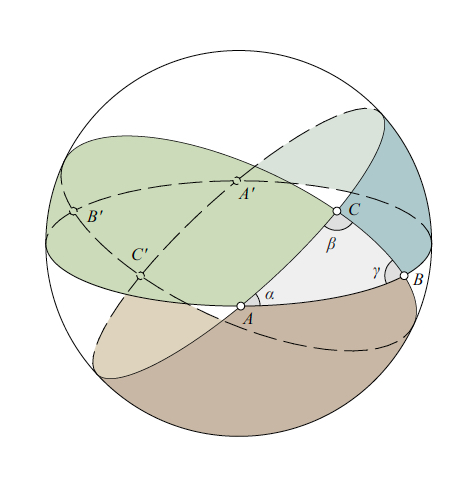
\includegraphics[width=0.4\textwidth]{kugel/Zweiecke.jpg}
    \captionof{figure}{Drei Grosskreise bilden ein sphärisches Dreieck}
\end{center}

In den nachstehenden Erklärungen und Herleitungen, sprechen wir ausschliesslich von Eulerschen’Dreiecken, da die umgeformten Winkelsätze der ebenen Trigonometrie nur auf diese Art von Kugeldreiecken angewendet werden kann.

$A_{ \overline{ ABC }}$ ist die Fläche des Dreieckes auf der Kugeloberfläche
In der ebenen Trigonometrie liegt die Winkelsumme eines Dreiecks bei
$180^{\circ}$.

Anders aber in der sphärischen Trigonometrie. Obschon sie einige Gemeinsamkeiten zur ebenen Trigonometrie aufweist, kann man nicht alles übernehmen.
So auch nicht wie Winkelsumme in einem sphärischen Dreieck.
Diese liegt bei:

\[
\begin{aligned}
\pi
&-
3\pi
&
&\text{\bigg \vert}
&
180^{\circ}
&-
540^{\circ}
\end{aligned}
\]

daraus lässt sich ableiten, das ein einzelner Winkel nicht grösser als $\pi$ oder $180^{\circ}$ sein darf. Ansonsten ist es kein Eulersches’Dreieck und wir dürfen die sphärische Trigonometrie nicht anwenden.\\
Wichtig anzumerken ist, dass die Seiten immer in Radiant beschrieben werden und nicht im Längenmass Meter wie wir es uns gewohnt sind. 
Bei den Dreiecksseiten handelt es sich um Kreisbögen und keine Strecken.

\section{Dreiecksfläche}

\begin{align*}
\text{Zweieck A}
&=
\overline{ABC} + \overline{A'BC} = 2 \alpha r^{ 2 } = A_{ \alpha }\\
\text{Zweieck B}
&=
\overline{ABC} + \overline{AB'C} = 2 \beta r^{ 2 } = A_{ \beta }\\
\text{Zweieck C}
&=
\overline{ABC} + \overline{ABC'} = 2 \gamma r^{ 2 } = A_{ \gamma }
\end{align*}

\begin{align*}
A_{ \alpha } + A_{ \beta } + A_{ \gamma } &= \frac{ 4\pi r^{ 2 } }{ 2 } + 2A_{ \overline{ ABC }} \\
2\alpha r^{ 2 } + 2\beta r^{ 2 } + 2\gamma r^{ 2 } &= \frac{ 4\pi r^{ 2 } }{ 2 } + 2A_{ \overline{ ABC }} \parallel:2\\
\alpha r^{ 2 } + \beta r^{ 2 } + \gamma r^{ 2 } &= \pi r^{ 2 } + A_{ \overline{ ABC }} \parallel-\pi r^{ 2 }\\
r^{ 2 }\left(\alpha + \beta + \gamma - \pi\right) &= A_{ \overline{ ABC }}
\end{align*}




\section{Sphärischer Exzess}
Die Winkelsumme sphärischer Dreiecke ist immer \textgreater \,  $\pi$.

\begin{align*}
\pi < \alpha + \beta + \gamma
\end{align*}

Der sphärische Exzess gibt dabei an, wie stark die Winkelsumme von $\pi$ abweicht.

\begin{align*}
\pi + \epsilon &= \alpha + \beta + \gamma \\
\epsilon &= \alpha + \beta + \gamma - \pi
\end{align*}

Würde der sphärische Exzess in der ebenen Trigonometrie angewendet, wäre dieser = 0. 
Bezieht man das auf die Erde und somit einer Kugel, kann man mit Hilfe eines beliebigen sphärischen Dreieckes und dessen Flächeninhalt auf den Radius der Kugel schliessen.

\subsection{Grenzfall - Satz von Legendre}

\begin{quote} \textit{Ein kleines sphärisches Dreieck kann näherungsweise 
wie ein ebenes Dreieck mit denselben Seiten berechnet 
werden, wenn alle Winkel des ebenen Dreiecks die um 
je ein Drittel des sphärischen Exzesses verminderten 
Winkel des sphärischen Dreiecks nimmt.} \end{quote}
\begin{flushright} - Adrien-Marie Legendre (1752-1833), Paris 1787
\end{flushright}x

Diese Aussage zeigt den Zusammenhang zwischen der 
Trigonometrie in der Ebene sowie in auf der Kugel
auf. Im speziellen bei sehr kleinen sphärischen 
Dreiecken ist die Winkelsumme nur unwesentlich 
grösser als $180^{\circ}$. Des Weiteren kann gesagt werden,
dass der sphärische Exzess gleichmässig auf alle
Winkel aufgeteilt wird.
Wichtig anzumerken ist, dass der Satz von Legendre 
für grosse, aber endliche Radien $r$ gilt.

%[SKIZZE GROSSER RADIUS/KLEINE KRÜMMUNG, KLEINER RADIUS/GROSSE KRÜMMUNG!!!!]
%


\section{Sphärisch Analoge Winkelfunktionen}

\subsection{Sphärischer Sinussatz}

Wir stellen die allgemeinen Sinussätze der Winkel $\alpha$ und $\gamma$ auf:


\[
\begin{aligned}
&{sin(\gamma)} = \frac{h}{a}
&
&\text{\bigg \vert}
&
&{sin(\alpha)} = \frac{h}{c}
&
\end{aligned}
\]

Daraus folgt:
\begin{align*}
h &= sin(\gamma)\cdot a \\
h &= sin(\alpha)\cdot c
\end{align*} 

Durch Gleichsetzung erhält man:
\begin{align*}
h &= h \\
sin(\gamma)\cdot a &= sin(\alpha)\cdot c
\end{align*} 

Durch umstellen erhalten wir den Sinussatz für a und c:
\begin{align*}
sin(\gamma)\cdot a &= sin(\alpha)\cdot c \\
\frac{sin(\gamma)}{c} &= \frac{sin(\alpha)}{a} 
\end{align*} 



\begin{align*}
\frac{sin(\alpha)}{sin(a)} = \frac{sin(\beta)}{sin(b)} = \frac{sin(\gamma)}{sin(c)}
\end{align*} 


\subsection{Winkelkosinussatz}

%[SKIZZE WINKELKOSINUS]

\[
\begin{aligned}
&\overline{C'A'} &= d\cdot {tan(b)}
&
&
&
&
&
&\overline{C'B'} &= d\cdot {tan(a)}
\end{aligned}
\]

\[
\begin{aligned}
&\overline{MA'} &= \frac{ d }{cos(b)}
&
&
&
&
&
&\overline{MB'} &= \frac{ d }{cos(a)}
\end{aligned}
\]

Der allgemeine Kosinussatz beschreibt sich wie folgt:

\begin{align*}
c^{ 2 } &= a^{ 2 } + b^{ 2 } - 2ab \cdot cos(\gamma)
\end{align*}

\begin{align*}
\triangle \overline{A'B'C' }
\overline{ A'B' }^{ 2 } &= \overline{ C'B' }^{ 2 } + \overline{ C'A' }^{ 2 } - 2 \cdot \overline{ C'B' } \cdot \overline{ C'A' } \cdot cos(\gamma)
\end{align*}



\begin{align*}
\overline{A'B'}^{ 2 } &= (d\cdot tan(a))^{ 2 } + (d\cdot tan(b))^{ 2 } - 2 \cdot (d\cdot tan(a) \cdot (d\cdot tan(b) \cdot cos(\gamma)\\
\overline{A'B'}^{ 2 } &= d^{ 2 } \cdot \left(\left(tan^{ 2 }(a) + tan^{ 2 }(b)\right) - 2\cdot tan(a) \cdot tan(b) \cdot cos(\gamma)\right)
\end{align*}

\begin{align*}
\triangle \overline{ MA'B' }
\overline{ A'B' }^{ 2 } &= \overline{ MB' }^{ 2 } + \overline{ MA' }^{ 2 } - 2\cdot \overline{ MB'} \cdot \overline{ MA' } \cdot cos(c)
\end{align*}


\begin{align*}
\overline{ A'B'}^{ 2 } &= \left(\frac{ d }{ cos(a) }  \right)^{ 2 } + \left(\frac{ d }{ cos(b)}  \right)^{ 2 } - 2 \cdot \frac{ d }{ cos(a)} \cdot \frac{ d }{ cos(b)} \cdot cos(c) \\
\overline{ A'B' }^{ 2 } &= d^{ 2 } \cdot \left(\left(\frac{ 1 }{ cos(a) }  \right)^{ 2 } + \left(\frac{ 1 }{ cos(b) }  \right)^{ 2 } - 2 \cdot \frac{ 1 }{ cos(a)} \cdot \frac{ 1 }{ cos(b)} \cdot cos(c)\right)\\
\overline{ A'B' }^{ 2 } &= d^{ 2 } \cdot \left(\left(tan^{ 2 }(a) + 1\right) + \left(tan^{ 2 }(b) + 1\right) - \left(2 \cdot \frac{cos(c)}{cos(a) \cdot cos(b)}\right)\right)
\end{align*}



\begin{align*}
\overline{ A'B'}^{ 2 } &= d^{ 2 } \cdot \left(\left(tan^{ 2 }(a) + tan^{ 2 }(b)\right) - 2 \cdot tan(a) \cdot tan(b) \cdot cos(\gamma)\right) \\
\overline{ A'B'}^{ 2 } &= d^{ 2 } \cdot \left(\left(tan^{ 2 }(a) + 1\right) + \left(tan^{ 2 }(b) + 1\right) - \left(2 \cdot \frac{cos(c)}{cos(a) \cdot cos(b)}\right)\right)
\end{align*}

Die anderen Gleichungen des Satzes, erfolgen aus Symmetriegründen.

\subsection{Seitenkosinussatz}
Durch zyklische Vertauschung des Winkelkosinus erhalten wir den Seitenkosinussatz:

\begin{align*}
{cos(a)} &= {cos(b)} \cdot {cos(c)} + {sin(b)} \cdot {sin(c)} \cdot {sin(\alpha)}\\
{cos(b)} &= {cos(a)} \cdot {cos(c)} + {sin(a)} \cdot {sin(c)} \cdot {sin(\beta)}\\
{cos(c)} &= {cos(a)} \cdot {cos(b)} + {sin(a)} \cdot {sin(b)} \cdot {sin(\gamma)}\\
\end{align*}

\section{Navigation auf See}
Das besondere an Seekarten ist die Inhaltliche Ausrichtung. Anders wie Landkarten muss sie Informationen enthalten welche für den Kapitän und seine Besatzung von grosser Bedeutung sind. Vor allem in Küstennähe ist das navigieren eines Schiffes besonders gefährlich. So enthalten Seekarten etwas über Wassertiefen, Bodenbeschaffenheiten, Gezeiten, Küstenlinien, Landzungen und Windrichtungen.
Der Hauptunterschied dabei ist, das auf der Landkarte feste Positionen definiert und aufgezeigt werden, das einzige was sich verändert ist der Reisende selbst. Bei der Seekarte ist das anders, es werden veränderliche Einwirkungen der Natur festgehalten.

Dieser kleine Unterschied zeigt die Notwendigkeit auf, die Position und den Kurs seines Schiffes auf See immer ermitteln zu können.


\section{Geographische Koordinaten}

Nachdem klar war, das die Erde eine Kugel ist, wurde diese in ein Gradnetz aufgeteilt. Dabei wurden die Angaben für eine exakte Ortsbestimmung klar definiert und die bis heute gültigen Koordinaten bestimmt.
Dabei muss man sich nochmals in Erinnerung rufen, dass sich die Erde in 24h einmal um ihre eigene Achse dreht. Nach $360 ^{\circ}$ 
und somit einer vollen Umdrehung, steht sie wieder in ihrer Ursprungsposition und ein neuer Tag beginnt.

Die Koordinaten setzen sich aus folgenden Komponenten zusammen:

\[
\begin{aligned}
&\text{Grad } (^{\circ})
&
&\text{\bigg \vert}
&
&\text{Bogenminuten } (`)
&
&\text{\bigg \vert}
&
&\text{Bogensekunden } (``)
\end{aligned}
\]

Die Erdoberfläche wurde in je 360 Breiten- und Längengrade eingeteilt. Die Breitengrade haben zueinander einen Abstand von 111.31 km, dies entspricht auch dem Abstand der Längengrade am Äquator mit Zunehmender Nähe zu den Polen, nimmt dieser Abstand ab.

\[
\begin{aligned}
&1^{\circ}
&
&\text{\bigg \vert}
&
&4 \text{ Minuten}
&
&\text{\bigg \vert}
&
&111.31\text{ km}
\end{aligned}
\]

Berechnet man nun die Erdumdrehung von 360°, erhält man genau den Erdumfang am Äquator: \begin{align*} 40’074 \text{ km.}\end{align*}

Dabei geben die Bogenminuten und -sekunden dem Standort die gewünschte Exaktheit. Mit den vollständigen Koordinaten lässt sich der Standort auf einer Landkarte exakt bestimmen und einzeichnen.

\subsection{Zeitzonen der Erde}
Wenn man nun die verschiedenen Zeitzonen der Erde betrachtet, macht die Verschiebung von jeweils einer Stunde durchaus Sinn, es lässt sich auf die Längengrade schliessen.
Zwischen den verschiedenen Zeitzonen liegen 15 Längengrade:

\begin{align*}
\text{15 Längengrade à 4 Minuten = 60 Minuten Zeitverschiebung = ca. 1665 km}
\end{align*}

Dabei ist die Zeitzone in welcher Mitte sich der Greenwich Meredian befindet die \textit{Greenwich Mean Time (GMT)} welche bis 1928 als Weltzeit galt. Im Jahr 1972 wurde diese umbenannt in die \textit{Coordinated Universal Time (UTC)} und wir von da an als Weltzeit $\pm$ 0.00 verwendet.


\section{Der Breitengrad}
Die Breitengrade bilden die bereits genannten Kleinkreise auf der Kugeloberfläche. Sie verlaufen in einem Abstand von genau 111 km parallel zum Äquator. Dabei stellt  dieser genau die Mitte zwischen Nord- und Südpol dar und teilt die Erdkugel in zwei gleiche Hälften. Somit wird von nördlicher und südlicher Breite gesprochen, je nach dem auf welcher Halbkugel man sich befindet.

%[SKIZZE DER GEOGRAFISCHEN BREITE ERDKUGEL]

\subsection{Geografische Breite $\phi$}
\begin{definition}
Die geografische Breite eines Standortes ist nichts anderes, als der Winkel am Erdmittelpunkt zwischen der Ebene des Äquators und der Geraden zum Standpunkt auf der Erdoberfläche.
\end{definition}

%[SKIZZE DER GEOGRAFISCHEN BREITE MIT WINKEL]

\subsection{Navigation mit den Breitengraden}
Da der Breitengrad bereits sehr früh ziemlich präzise bestimmt werden könnte, nutzten bereits die Seefahrer um Christoph Kolumbus den Breitengrad zur Navigation ihrer Flotten.
Den dieser lässt sich ziemlich einfach aus dem höchsten Sonnenstand oder einem Fixstern bestimmen. Dabei wird mit einem Jakobsstab\footnote{%
Der Jakobsstab ist ein früheres astronomisches Instrument zur Winkelmessung und wurde vor allem in der Seefahrt verwendet. Er ist in der Nautik der Vorläufer des Sextanten.} (später Sextant\footnote{%
Der Sextant ist ein nautisches Messinstrument zur Winkelmessung von Horizont und Fixstern (Gestirn)}) der Winkel zwischen dem Horizont und dem Fixstern gemessen. Der Winkel welchen man erhält, zieht man von 90° ab und erhält somit die geografische Breite. \\

%[SKIZZE ERMITTLUNG DES BREITENGRADES]

Wenn man sich auf der Nordhalbkugel befindet, ist der Polarstern ein sehr guter Fixstern. Befindet sich ein Schiff nun sehr nahe am Nordpol, steht dieser nahezu senkrecht am Himmelszelt bei $90^{\circ}$. Würde es aber nahe dem Äquator stehen, erscheint dieser am Horizont bei $0^{\circ}$.

\subsection{Korrekturbeiwert}

\section{Der Längengrad}
Die Längengrade bilden die bereits genannten Grosskreise auf der Kugeloberfläche.
Sie schneiden den Äquator im rechten Winkel, haben dort einen Abstand von 111 km zueinander und verbinden die Pole. Anders wie bei der geografischen Breite, ist in der Natur kein Längengrad gegeben welcher den Nullpunkt darstellt.

%[SKIZZE DER GEOGRAFISCHEN LÄNGE ERDKUGEL]

\subsection{Geografische Länge $\lambda$}
\begin{definition}
Die geografische Länge ist der Winkel an der Erdachse zum Nullmeridian.
\end{definition}

\subsection{Navigation mit den Längengraden}
Die geografische Länge lässt sich nicht so einfach bestimmen wie deren Breite. Für die Berechnung auf See benötigt man eine Referenzzeit eines Ortes mit bekannter Länge.
In der Zeit der Entdecker gab es noch keine mechanischen Uhren. Die Sonnenuhr war zudem ungeeignet, da diese nur die Uhrzeit am Standort mass und nicht die am Referenzort selbst. Die erste Pendeluhr wurde erst Mitte des 17. Jahrhunderts erfunden, was in der Schifffahrt aber auch nicht die Lösung brachte.\\
Pendeluhren auf einem Schiff sind ungeeignet, da das Pendel mit dem Wellengang aus dem Takt gebracht wird und somit die Uhr falsch geht.
Zu ungenau und gegen äussere Erschütterungen zu empfindlich waren später auch die federgetriebenen Uhren und die Unruh. Dazukamen die verschiedenen Klimazonen welche ein Schiff zu durchqueren hatten. Das Metall zog sich viel zu fest zusammen oder dehnte sich aus, was dazu führte das die Uhr unregelmässig lief.

Das sogenannte „Längenproblem“ stellte nicht nur bei der Navigation auf See ein Problem dar, es ergaben sich auch wirtschaftliche Konsequenzen. Die Schiffe mussten bis zur gewünschten geografischen Breite navigieren und segelten dann den Breitengrad entlang. Dabei waren die Schiffe oft Wochenlang unterwegs und segelten die „Breiten ab“ um an die gewünschte Position zu kommen. Dies führte zu erheblichen Zeitverlusten und viel längeren Reisezeiten.


\section{The Board of Longitude - Das Längenproblem}
Das Längenproblem beschäftigte alle grossen Seefahrernationen Europas. Wenn man bedenkt das sich Werte in einer  Höhe von halben britischen Staatshaushalten auf verloren gegangenen Schiffen befanden, erkennt man die Dringlichkeit für eine zuverlässige und genaue Navigation auf See.


\begin{itemize}
\item £ 20’000 - Abweichung von max. einem halben Grad
\item £ 15’000 - Abweichung von zwei Drittel Grad
\item £ 10’000 - Abweichung von max. $1 ^{\circ}$
\end{itemize}

\subsection{John Harrison}


\subsection{Tobias Mayer}



Uhren mit einer Abweichung von einer Minute Abweichung pro Tag (





\section{Nautische Dreieck}


$\Rightarrow$





\section{Die Vermessung der Welt}
Wir schreiben das Jahr 1818 und kehren in die Zeit des Mathematikers Carl Friedrich Gauss zurück. Neben dem liebevoll genannten „kleinen Gauss“ und anderen herausragenden Mathematischen Leistungen, beschäftigte er in den Folgejahren mit der Vermessung des Königreichs Hannovers und verfasste auf 61 Blättern das Kartenwerk \textit{Gauss’sche Landesaufnahme der 1815 durch Hannover erworbenen Gebiete}.






AUFGABE

Hubble Teleskop 
24. April 1990






\printbibliography[heading=subbibliography]
\end{refsection}




%\chapter{Geometrie auf der Kugeloberfläche\label{chapter:kugel}}
\lhead{Geometrie auf der Kugeloberfläche}
\begin{refsection}
\chapterauthor{Melina Staub und Fabian Schmid}

\section{Einleitung}

Schon seit jeher fasziniert den Menschen die Fahrt zur See. Nicht grundlos ist die Seefahrt eine der wichtigsten und ältesten Tätigkeiten der Menschheit. Der innerliche Drang neue Weltmeere und unbekannte Gebiete zu entdecken, die Fahrt zur See zu erleichtern und erträglicher zu machen, trieben die Menschen an, die Schiffe dieser Welt immer weiter zu entwickeln.

Die Idee der Kugelform der Erde ist älter als man zu denken vermag. Bereits der Schüler des antiken griechischen Philosophen Platon - Aristoteles schrieb in seiner Schrift \textit{Über den Himmel} aus dem 4. Jahrhundert v. Chr. etliche Gründe welche für die Gestallt der Erde als Kugel sprechen:

\begin{itemize}
      \item Sämtliche schweren Körper streben zum Mittelpunkt des Alls. Da sie dies von allen Seiten her gleichmäßig tun und die Erde im Mittelpunkt des Alls steht, muss sie eine kugelrunde Gestalt annehmen. 
\item Bei von der Küste wegfahrende Schiffen wird der Rumpf vor den Segeln der Sicht verborgen. 
\item In südlichen Ländern erscheinen südliche Sternbilder höher über dem Horizont.
\item Der Erdschatten bei einer Mondfinsternis ist stets rund.
\end{itemize}

Jedoch war um 1492 - der Zeit der Entdeckung Amerikas durch Christoph Kolumbus, die Idee der Erde in Kugelform noch sehr umstritten. Er erkannte anhand den Theorien und Erkenntnissen der alten Griechen, vor allem Aristoteles, das die Erde eine Kugel sein muss. \\
Doch mit seinem Vorschlag einen Seeweg über den Atlantik nach Indien zu finden und nicht wie üblich um Afrika zu segeln, stiess er beim beim portugiesischen König auf taube Ohren. Sein Plan Indien über eine Route nach Westen zu erreichen, widersprach dem gesunden Menschenverstand. Wäre die Erde wirklich eine Kugel und man befände sich auf der unteren Erdhalbkugel, würde man herunterfallen.\\
Doch auch der damals übliche Glaube an die Erde in Scheibenform brachte so einige Risiken mit sich. Was würde passieren, wenn die Flotte das Ende der Scheibe erreicht hatte? Würden sie über den Erdrand hinweggleiten und in den Abgrund stürzen?\\
Erst nach viel Überzeugungsarbeit durch Kolumbus, setzte er sich am Spanischen Hof durch und segelte über die Westliche Route über den Atlantik und entdeckte schlussendlich Amerika.

Der praktische und greifbare Beweis das die Erde eine Kugel ist, lieferte rund 30 Jahre später der Portugiese Fernando Magellan. Mit seiner Weltumsegelung und seiner Ankunft in den Philippinen, bewies er definitiv das die Erde eine Kugel ist.\\

Nun wollen wir uns die Frage stellen, wie die alten Seefahrer ohne GPS und jeglichen modernen Navigationssystemen auf hoher See wussten wo sie sich befinden und was haben die Sterne mit alldem zu tun? Reisen Sie mit uns zurück in eine Zeit mit Sextant, Kompass und Sternkarten. In die Zeit der Seefahrer und Entdecker.


\section{Geometrie auf der Ebene und der Kugel}

Euklid von Alexandria beschrieb die Grundbegriffe der ebenen Geometrie mittels Punkt, Geraden, Ebene, Winkel und Dreieck. Diese Dreiecke lassen sich mithilfe der ebenen Trigonometrie beschreiben. Dabei gelten die uns bekannten trigonometrischen Winkelfunktionen:\\

\text{Sinussatz:}
\begin{align*}
\frac{ a }{ sin(\alpha) } &= \frac{ b }{sin(\beta)} = \frac{ c }{ sin(\gamma) } = \frac{abc}{2A} = 2r\\
\end{align*}

\text{Cosinussatz:}
\begin{align*}
c^{ 2 } &= a^{ 2 } + b^{ 2 } - 2ab\cdot cos(\gamma)\\
b^{ 2 } &= a^{ 2 } + c^{ 2 } - 2ab\cdot cos(\beta)\\
a^{ 2 } &= b^{ 2 } + c^{ 2 } - 2ab\cdot cos(\alpha)
\end{align*}

Um Dreiecke auf der Kugeloberfläche zu berechnen, benötigt man die sphärische Trigonometrie. Die oben beschriebenen Sätze lassen sich auf der Kugel nicht anwenden, sie werden aber als Grundlage zur Herleitung der Sätze für das Kugeldreieck benötigt.

Die nachfolgenden Seiten thematisieren die Geometrie auf der Kugeloberfläche und wie sie in der Navigation eingesetzt werden kann.


\section{Gross- und Kleinkreise}

Eine Kugeloberfläche lässt sich in zwei verschiedene Kreisarten einteilen -  Gross- und Kleinkreise. 
Wir betrachten als erstes die Grosskreise:

\begin{definition}
Ein Großkreis ist ein größtmöglicher Kreis auf einer Kugeloberfläche. Sein Mittelpunkt fällt immer mit dem Mittelpunkt der Kugel zusammen und ein Schnitt auf dem Großkreis teilt die Kugel in jedem Fall in zwei („gleich große“) Hälften.
\end{definition}

Es gibt unendlich viele Möglichkeiten, eine Kugel in zwei gleich grosse Stücke zu zerschneiden, 
daher gibt es auch unendlich viele Grosskreise. Wenn wir die Grosskreise auf einer Kugel mit diesen auf der Erde beschreiben, sprechen wir von den Längengraden aber auch der Äquator beschreibt einen Grosskreis.
Ein Elementarer Bestandteil bilden die Grosskreise in der sphärischen Trigonometrie. Mithilfe der Schnittpunkte verschiedener Grosskreise, lässt sich ein Sphärisches Dreieck bilden auf welchem sich die sphärische Trigonometrie anwenden lässt.

[GRAFIK GROSSKREISE]

\begin{definition}
Unter Kleinkreis versteht man jene Kreise auf einer Kugeloberfläche, deren Ebenen nicht den Kugelmittelpunkt enthalten.
\end{definition}

Die Kleinkreise eignen sich im Gegensatz zu den Grosskreisen \textit{nicht} für die sphärische Trigonometrie. 
Sie werden lediglich zur Bestimmung der Messgrössen, Winkelabstände oder des Höhenwinkels eines Gestirns verwendet. 

Wenn wir die Kleinkreise auf die Erdoberfläche projizieren betrachten wir die Breitengrade.

[GRAFIK KLEINKREISE]


\section{Sphärische Dreiecke / Kugeldreieck}

\begin{center}
        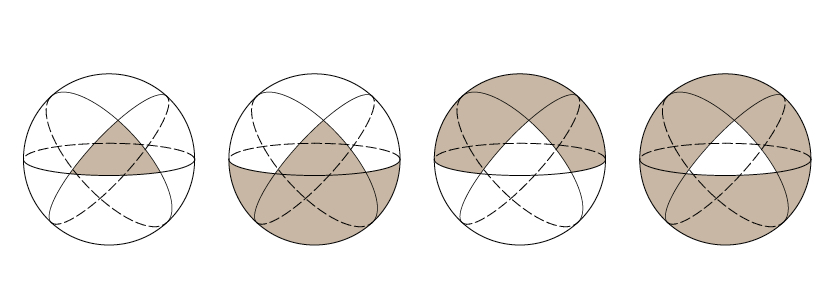
\includegraphics[width=0.9\textwidth]{kugel/Dreieckarten.jpg}
    \captionof{figure}{Dreieckarten auf einer Kugeloberfläche}
\end{center}

Der Begriff Sphärisches Dreieck oder Kugeldreieck ist ein sehr weitläufiger Begriff. 
Dabei können wir den Begriff in drei für uns wesentliche Dreiecke unterteilen:

\begin{itemize}
\item Kugelzweieck
\item Nicht Eulersche’Dreiecke
\item Eulersche’Dreiecke
\end{itemize}

\subsection{Kugelzweieck}

Zwei Grosskreise auf der Kugeloberfläche, zerlegen diese in vier gleiche Kugelzweiecke. 
Jedes dieser Dreieckseiten hat die Länge
$180^{\circ}$ oder $\pi$
Der Flächeninhalt wird dabei nur durch den Winkel $\alpha$ zwischen den beiden Grosskreisen bestimmt.

\begin{center}
        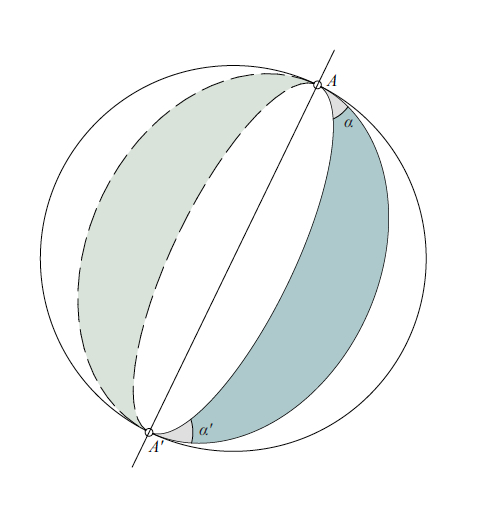
\includegraphics[width=0.3\textwidth]{kugel/Zweieck.jpg}
    \captionof{figure}{Bildung von Zweiecken durch Grosskreise}
\end{center}

Dabei ist der Flächeninhalt der ganzen Kugel:

\begin{align*}
A_{ Kugel } &= 4 \pi r^{2}
\end{align*}


Um den Flächeninhalt des betrachteten Zweieckes zu bekommen, 
müssen wir das ganze noch mit dem Kugelsegment mit dem Winkel $\alpha$ multiplizieren.

\begin{align*}
A_{ Zweieck } &= 4 \pi r^{2} \cdot \frac{ \alpha }{ 2 \pi }
\end{align*}


\subsection{Nicht Eulersche’ Dreiecke}

BLABLA

\subsection{Eulersche’ Dreiecke}

Legt man drei Grosskreise auf eine Kugeloberfläche, bilden sich dabei acht Dreiecke. 
Ein solches Dreieck heisst Eulersches’Dreieck\footnote{%
Leonard Euler (1707-1783), berühmter Schweizer Mathematiker und Physiker. 
Nicht Eulersche’Dreiecke erhält man, indem man das Äussere des Dreieckes ABC betrachtet.} 
Diese Dreiecke werden weder durch die Verlängerung ihrer Seiten durchschnitten, 
noch haben sie Dreiecksseiten welche grösser als $180^{\circ}$ sind.

\begin{center}
        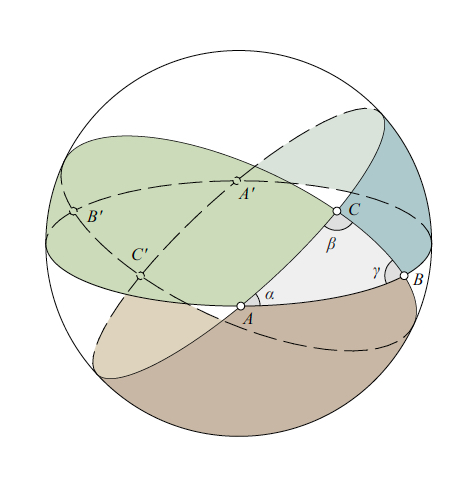
\includegraphics[width=0.4\textwidth]{kugel/Zweiecke.jpg}
    \captionof{figure}{Drei Grosskreise bilden ein sphärisches Dreieck}
\end{center}

In den nachstehenden Erklärungen und Herleitungen, sprechen wir ausschliesslich von Eulerschen’Dreiecken, da die umgeformten Winkelsätze der ebenen Trigonometrie nur auf diese Art von Kugeldreiecken angewendet werden kann.

$A_{ \overline{ ABC }}$ ist die Fläche des Dreieckes auf der Kugeloberfläche
In der ebenen Trigonometrie liegt die Winkelsumme eines Dreiecks bei
$180^{\circ}$.

Anders aber in der sphärischen Trigonometrie. Obschon sie einige Gemeinsamkeiten zur ebenen Trigonometrie aufweist, kann man nicht alles übernehmen.
So auch nicht wie Winkelsumme in einem sphärischen Dreieck.
Diese liegt bei:

\[
\begin{aligned}
\pi
&-
3\pi
&
&\text{\bigg \vert}
&
180^{\circ}
&-
540^{\circ}
\end{aligned}
\]

daraus lässt sich ableiten, das ein einzelner Winkel nicht grösser als $\pi$ oder $180^{\circ}$ sein darf. Ansonsten ist es kein Eulersches’Dreieck und wir dürfen die sphärische Trigonometrie nicht anwenden.\\
Wichtig anzumerken ist, dass die Seiten immer in Radiant beschrieben werden und nicht im Längenmass Meter wie wir es uns gewohnt sind. 
Bei den Dreiecksseiten handelt es sich um Kreisbögen und keine Strecken.

\section{Dreiecksfläche}

\begin{align*}
\text{Zweieck A}
&=
\overline{ABC} + \overline{A'BC} = 2 \alpha r^{ 2 } = A_{ \alpha }\\
\text{Zweieck B}
&=
\overline{ABC} + \overline{AB'C} = 2 \beta r^{ 2 } = A_{ \beta }\\
\text{Zweieck C}
&=
\overline{ABC} + \overline{ABC'} = 2 \gamma r^{ 2 } = A_{ \gamma }
\end{align*}

\begin{align*}
A_{ \alpha } + A_{ \beta } + A_{ \gamma } &= \frac{ 4\pi r^{ 2 } }{ 2 } + 2A_{ \overline{ ABC }} \\
2\alpha r^{ 2 } + 2\beta r^{ 2 } + 2\gamma r^{ 2 } &= \frac{ 4\pi r^{ 2 } }{ 2 } + 2A_{ \overline{ ABC }} \parallel:2\\
\alpha r^{ 2 } + \beta r^{ 2 } + \gamma r^{ 2 } &= \pi r^{ 2 } + A_{ \overline{ ABC }} \parallel-\pi r^{ 2 }\\
r^{ 2 }\left(\alpha + \beta + \gamma - \pi\right) &= A_{ \overline{ ABC }}
\end{align*}




\section{Sphärischer Exzess}
Die Winkelsumme sphärischer Dreiecke ist immer \textgreater \,  $\pi$.

\begin{align*}
\pi < \alpha + \beta + \gamma
\end{align*}

Der sphärische Exzess gibt dabei an, wie stark die Winkelsumme von $\pi$ abweicht.

\begin{align*}
\pi + \epsilon &= \alpha + \beta + \gamma \\
\epsilon &= \alpha + \beta + \gamma - \pi
\end{align*}

Würde der sphärische Exzess in der ebenen Trigonometrie angewendet, wäre dieser = 0. 
Bezieht man das auf die Erde und somit einer Kugel, kann man mit Hilfe eines beliebigen sphärischen Dreieckes und dessen Flächeninhalt auf den Radius der Kugel schliessen.

\subsection{Grenzfall - Satz von Legendre}

\begin{quote} \textit{Ein kleines sphärisches Dreieck kann näherungsweise 
wie ein ebenes Dreieck mit denselben Seiten berechnet 
werden, wenn alle Winkel des ebenen Dreiecks die um 
je ein Drittel des sphärischen Exzesses verminderten 
Winkel des sphärischen Dreiecks nimmt.} \end{quote}
\begin{flushright} - Adrien-Marie Legendre (1752-1833), Paris 1787
\end{flushright}x

Diese Aussage zeigt den Zusammenhang zwischen der 
Trigonometrie in der Ebene sowie in auf der Kugel
auf. Im speziellen bei sehr kleinen sphärischen 
Dreiecken ist die Winkelsumme nur unwesentlich 
grösser als $180^{\circ}$. Des Weiteren kann gesagt werden,
dass der sphärische Exzess gleichmässig auf alle
Winkel aufgeteilt wird.
Wichtig anzumerken ist, dass der Satz von Legendre 
für grosse, aber endliche Radien $r$ gilt.

%[SKIZZE GROSSER RADIUS/KLEINE KRÜMMUNG, KLEINER RADIUS/GROSSE KRÜMMUNG!!!!]
%


\section{Sphärisch Analoge Winkelfunktionen}

\subsection{Sphärischer Sinussatz}

Wir stellen die allgemeinen Sinussätze der Winkel $\alpha$ und $\gamma$ auf:


\[
\begin{aligned}
&{sin(\gamma)} = \frac{h}{a}
&
&\text{\bigg \vert}
&
&{sin(\alpha)} = \frac{h}{c}
&
\end{aligned}
\]

Daraus folgt:
\begin{align*}
h &= sin(\gamma)\cdot a \\
h &= sin(\alpha)\cdot c
\end{align*} 

Durch Gleichsetzung erhält man:
\begin{align*}
h &= h \\
sin(\gamma)\cdot a &= sin(\alpha)\cdot c
\end{align*} 

Durch umstellen erhalten wir den Sinussatz für a und c:
\begin{align*}
sin(\gamma)\cdot a &= sin(\alpha)\cdot c \\
\frac{sin(\gamma)}{c} &= \frac{sin(\alpha)}{a} 
\end{align*} 



\begin{align*}
\frac{sin(\alpha)}{sin(a)} = \frac{sin(\beta)}{sin(b)} = \frac{sin(\gamma)}{sin(c)}
\end{align*} 


\subsection{Winkelkosinussatz}

%[SKIZZE WINKELKOSINUS]

\[
\begin{aligned}
&\overline{C'A'} &= d\cdot {tan(b)}
&
&
&
&
&
&\overline{C'B'} &= d\cdot {tan(a)}
\end{aligned}
\]

\[
\begin{aligned}
&\overline{MA'} &= \frac{ d }{cos(b)}
&
&
&
&
&
&\overline{MB'} &= \frac{ d }{cos(a)}
\end{aligned}
\]

Der allgemeine Kosinussatz beschreibt sich wie folgt:

\begin{align*}
c^{ 2 } &= a^{ 2 } + b^{ 2 } - 2ab \cdot cos(\gamma)
\end{align*}

\begin{align*}
\triangle \overline{A'B'C' }
\overline{ A'B' }^{ 2 } &= \overline{ C'B' }^{ 2 } + \overline{ C'A' }^{ 2 } - 2 \cdot \overline{ C'B' } \cdot \overline{ C'A' } \cdot cos(\gamma)
\end{align*}



\begin{align*}
\overline{A'B'}^{ 2 } &= (d\cdot tan(a))^{ 2 } + (d\cdot tan(b))^{ 2 } - 2 \cdot (d\cdot tan(a) \cdot (d\cdot tan(b) \cdot cos(\gamma)\\
\overline{A'B'}^{ 2 } &= d^{ 2 } \cdot \left(\left(tan^{ 2 }(a) + tan^{ 2 }(b)\right) - 2\cdot tan(a) \cdot tan(b) \cdot cos(\gamma)\right)
\end{align*}

\begin{align*}
\triangle \overline{ MA'B' }
\overline{ A'B' }^{ 2 } &= \overline{ MB' }^{ 2 } + \overline{ MA' }^{ 2 } - 2\cdot \overline{ MB'} \cdot \overline{ MA' } \cdot cos(c)
\end{align*}


\begin{align*}
\overline{ A'B'}^{ 2 } &= \left(\frac{ d }{ cos(a) }  \right)^{ 2 } + \left(\frac{ d }{ cos(b)}  \right)^{ 2 } - 2 \cdot \frac{ d }{ cos(a)} \cdot \frac{ d }{ cos(b)} \cdot cos(c) \\
\overline{ A'B' }^{ 2 } &= d^{ 2 } \cdot \left(\left(\frac{ 1 }{ cos(a) }  \right)^{ 2 } + \left(\frac{ 1 }{ cos(b) }  \right)^{ 2 } - 2 \cdot \frac{ 1 }{ cos(a)} \cdot \frac{ 1 }{ cos(b)} \cdot cos(c)\right)\\
\overline{ A'B' }^{ 2 } &= d^{ 2 } \cdot \left(\left(tan^{ 2 }(a) + 1\right) + \left(tan^{ 2 }(b) + 1\right) - \left(2 \cdot \frac{cos(c)}{cos(a) \cdot cos(b)}\right)\right)
\end{align*}



\begin{align*}
\overline{ A'B'}^{ 2 } &= d^{ 2 } \cdot \left(\left(tan^{ 2 }(a) + tan^{ 2 }(b)\right) - 2 \cdot tan(a) \cdot tan(b) \cdot cos(\gamma)\right) \\
\overline{ A'B'}^{ 2 } &= d^{ 2 } \cdot \left(\left(tan^{ 2 }(a) + 1\right) + \left(tan^{ 2 }(b) + 1\right) - \left(2 \cdot \frac{cos(c)}{cos(a) \cdot cos(b)}\right)\right)
\end{align*}

Die anderen Gleichungen des Satzes, erfolgen aus Symmetriegründen.

\subsection{Seitenkosinussatz}
Durch zyklische Vertauschung des Winkelkosinus erhalten wir den Seitenkosinussatz:

\begin{align*}
{cos(a)} &= {cos(b)} \cdot {cos(c)} + {sin(b)} \cdot {sin(c)} \cdot {sin(\alpha)}\\
{cos(b)} &= {cos(a)} \cdot {cos(c)} + {sin(a)} \cdot {sin(c)} \cdot {sin(\beta)}\\
{cos(c)} &= {cos(a)} \cdot {cos(b)} + {sin(a)} \cdot {sin(b)} \cdot {sin(\gamma)}\\
\end{align*}

\section{Navigation auf See}
Das besondere an Seekarten ist die Inhaltliche Ausrichtung. Anders wie Landkarten muss sie Informationen enthalten welche für den Kapitän und seine Besatzung von grosser Bedeutung sind. Vor allem in Küstennähe ist das navigieren eines Schiffes besonders gefährlich. So enthalten Seekarten etwas über Wassertiefen, Bodenbeschaffenheiten, Gezeiten, Küstenlinien, Landzungen und Windrichtungen.
Der Hauptunterschied dabei ist, das auf der Landkarte feste Positionen definiert und aufgezeigt werden, das einzige was sich verändert ist der Reisende selbst. Bei der Seekarte ist das anders, es werden veränderliche Einwirkungen der Natur festgehalten.

Dieser kleine Unterschied zeigt die Notwendigkeit auf, die Position und den Kurs seines Schiffes auf See immer ermitteln zu können.


\section{Geographische Koordinaten}

Nachdem klar war, das die Erde eine Kugel ist, wurde diese in ein Gradnetz aufgeteilt. Dabei wurden die Angaben für eine exakte Ortsbestimmung klar definiert und die bis heute gültigen Koordinaten bestimmt.
Dabei muss man sich nochmals in Erinnerung rufen, dass sich die Erde in 24h einmal um ihre eigene Achse dreht. Nach $360 ^{\circ}$ 
und somit einer vollen Umdrehung, steht sie wieder in ihrer Ursprungsposition und ein neuer Tag beginnt.

Die Koordinaten setzen sich aus folgenden Komponenten zusammen:

\[
\begin{aligned}
&\text{Grad } (^{\circ})
&
&\text{\bigg \vert}
&
&\text{Bogenminuten } (`)
&
&\text{\bigg \vert}
&
&\text{Bogensekunden } (``)
\end{aligned}
\]

Die Erdoberfläche wurde in je 360 Breiten- und Längengrade eingeteilt. Die Breitengrade haben zueinander einen Abstand von 111.31 km, dies entspricht auch dem Abstand der Längengrade am Äquator mit Zunehmender Nähe zu den Polen, nimmt dieser Abstand ab.

\[
\begin{aligned}
&1^{\circ}
&
&\text{\bigg \vert}
&
&4 \text{ Minuten}
&
&\text{\bigg \vert}
&
&111.31\text{ km}
\end{aligned}
\]

Berechnet man nun die Erdumdrehung von 360°, erhält man genau den Erdumfang am Äquator: \begin{align*} 40’074 \text{ km.}\end{align*}

Dabei geben die Bogenminuten und -sekunden dem Standort die gewünschte Exaktheit. Mit den vollständigen Koordinaten lässt sich der Standort auf einer Landkarte exakt bestimmen und einzeichnen.

\subsection{Zeitzonen der Erde}
Wenn man nun die verschiedenen Zeitzonen der Erde betrachtet, macht die Verschiebung von jeweils einer Stunde durchaus Sinn, es lässt sich auf die Längengrade schliessen.
Zwischen den verschiedenen Zeitzonen liegen 15 Längengrade:

\begin{align*}
\text{15 Längengrade à 4 Minuten = 60 Minuten Zeitverschiebung = ca. 1665 km}
\end{align*}

Dabei ist die Zeitzone in welcher Mitte sich der Greenwich Meredian befindet die \textit{Greenwich Mean Time (GMT)} welche bis 1928 als Weltzeit galt. Im Jahr 1972 wurde diese umbenannt in die \textit{Coordinated Universal Time (UTC)} und wir von da an als Weltzeit $\pm$ 0.00 verwendet.


\section{Der Breitengrad}
Die Breitengrade bilden die bereits genannten Kleinkreise auf der Kugeloberfläche. Sie verlaufen in einem Abstand von genau 111 km parallel zum Äquator. Dabei stellt  dieser genau die Mitte zwischen Nord- und Südpol dar und teilt die Erdkugel in zwei gleiche Hälften. Somit wird von nördlicher und südlicher Breite gesprochen, je nach dem auf welcher Halbkugel man sich befindet.

%[SKIZZE DER GEOGRAFISCHEN BREITE ERDKUGEL]

\subsection{Geografische Breite $\phi$}
\begin{definition}
Die geografische Breite eines Standortes ist nichts anderes, als der Winkel am Erdmittelpunkt zwischen der Ebene des Äquators und der Geraden zum Standpunkt auf der Erdoberfläche.
\end{definition}

%[SKIZZE DER GEOGRAFISCHEN BREITE MIT WINKEL]

\subsection{Navigation mit den Breitengraden}
Da der Breitengrad bereits sehr früh ziemlich präzise bestimmt werden könnte, nutzten bereits die Seefahrer um Christoph Kolumbus den Breitengrad zur Navigation ihrer Flotten.
Den dieser lässt sich ziemlich einfach aus dem höchsten Sonnenstand oder einem Fixstern bestimmen. Dabei wird mit einem Jakobsstab\footnote{%
Der Jakobsstab ist ein früheres astronomisches Instrument zur Winkelmessung und wurde vor allem in der Seefahrt verwendet. Er ist in der Nautik der Vorläufer des Sextanten.} (später Sextant\footnote{%
Der Sextant ist ein nautisches Messinstrument zur Winkelmessung von Horizont und Fixstern (Gestirn)}) der Winkel zwischen dem Horizont und dem Fixstern gemessen. Der Winkel welchen man erhält, zieht man von 90° ab und erhält somit die geografische Breite. \\

%[SKIZZE ERMITTLUNG DES BREITENGRADES]

Wenn man sich auf der Nordhalbkugel befindet, ist der Polarstern ein sehr guter Fixstern. Befindet sich ein Schiff nun sehr nahe am Nordpol, steht dieser nahezu senkrecht am Himmelszelt bei $90^{\circ}$. Würde es aber nahe dem Äquator stehen, erscheint dieser am Horizont bei $0^{\circ}$.

\subsection{Korrekturbeiwert}

\section{Der Längengrad}
Die Längengrade bilden die bereits genannten Grosskreise auf der Kugeloberfläche.
Sie schneiden den Äquator im rechten Winkel, haben dort einen Abstand von 111 km zueinander und verbinden die Pole. Anders wie bei der geografischen Breite, ist in der Natur kein Längengrad gegeben welcher den Nullpunkt darstellt.

%[SKIZZE DER GEOGRAFISCHEN LÄNGE ERDKUGEL]

\subsection{Geografische Länge $\lambda$}
\begin{definition}
Die geografische Länge ist der Winkel an der Erdachse zum Nullmeridian.
\end{definition}

\subsection{Navigation mit den Längengraden}
Die geografische Länge lässt sich nicht so einfach bestimmen wie deren Breite. Für die Berechnung auf See benötigt man eine Referenzzeit eines Ortes mit bekannter Länge.
In der Zeit der Entdecker gab es noch keine mechanischen Uhren. Die Sonnenuhr war zudem ungeeignet, da diese nur die Uhrzeit am Standort mass und nicht die am Referenzort selbst. Die erste Pendeluhr wurde erst Mitte des 17. Jahrhunderts erfunden, was in der Schifffahrt aber auch nicht die Lösung brachte.\\
Pendeluhren auf einem Schiff sind ungeeignet, da das Pendel mit dem Wellengang aus dem Takt gebracht wird und somit die Uhr falsch geht.
Zu ungenau und gegen äussere Erschütterungen zu empfindlich waren später auch die federgetriebenen Uhren und die Unruh. Dazukamen die verschiedenen Klimazonen welche ein Schiff zu durchqueren hatten. Das Metall zog sich viel zu fest zusammen oder dehnte sich aus, was dazu führte das die Uhr unregelmässig lief.

Das sogenannte „Längenproblem“ stellte nicht nur bei der Navigation auf See ein Problem dar, es ergaben sich auch wirtschaftliche Konsequenzen. Die Schiffe mussten bis zur gewünschten geografischen Breite navigieren und segelten dann den Breitengrad entlang. Dabei waren die Schiffe oft Wochenlang unterwegs und segelten die „Breiten ab“ um an die gewünschte Position zu kommen. Dies führte zu erheblichen Zeitverlusten und viel längeren Reisezeiten.


\section{The Board of Longitude - Das Längenproblem}
Das Längenproblem beschäftigte alle grossen Seefahrernationen Europas. Wenn man bedenkt das sich Werte in einer  Höhe von halben britischen Staatshaushalten auf verloren gegangenen Schiffen befanden, erkennt man die Dringlichkeit für eine zuverlässige und genaue Navigation auf See.


\begin{itemize}
\item £ 20’000 - Abweichung von max. einem halben Grad
\item £ 15’000 - Abweichung von zwei Drittel Grad
\item £ 10’000 - Abweichung von max. $1 ^{\circ}$
\end{itemize}

\subsection{John Harrison}


\subsection{Tobias Mayer}



Uhren mit einer Abweichung von einer Minute Abweichung pro Tag (





\section{Nautische Dreieck}


$\Rightarrow$





\section{Die Vermessung der Welt}
Wir schreiben das Jahr 1818 und kehren in die Zeit des Mathematikers Carl Friedrich Gauss zurück. Neben dem liebevoll genannten „kleinen Gauss“ und anderen herausragenden Mathematischen Leistungen, beschäftigte er in den Folgejahren mit der Vermessung des Königreichs Hannovers und verfasste auf 61 Blättern das Kartenwerk \textit{Gauss’sche Landesaufnahme der 1815 durch Hannover erworbenen Gebiete}.






AUFGABE

Hubble Teleskop 
24. April 1990






\printbibliography[heading=subbibliography]
\end{refsection}




\vfill
\pagebreak
\ifodd\value{page}\else\null\clearpage\fi
\lhead{Index}
\rhead{}
\addcontentsline{toc}{chapter}{\indexname}
%
% skript.tex -- Skript ueber Differentialgleichungen
%
% (c) 2014 Prof. Dr. Andreas Mueller, HSR
%
\documentclass{book}
\usepackage{etex}
\usepackage{geometry}
\geometry{papersize={170mm,240mm},total={140mm,200mm},top=21mm,bindingoffset=10mm}
\usepackage[english,ngerman]{babel}
\usepackage[utf8]{inputenc}
\usepackage{cancel}
\usepackage{times}
\usepackage{amsmath,amscd}
\usepackage{amssymb}
\usepackage{amsfonts}
\usepackage{amsthm}
\usepackage[nolist]{acronym}
\usepackage{graphicx}
\usepackage{fancyhdr}
\usepackage{textcomp}
\usepackage[all]{xy}
\usepackage{txfonts}
\usepackage{alltt} 
\usepackage{verbatim}
\usepackage{paralist}
\usepackage{makeidx}
\usepackage{array}
%\usepackage[colorlinks=true]{hyperref}
\usepackage{hyperref}
\usepackage{tikz}
\usepackage{pgfplots}
\usepackage{pgfplotstable}
\usepackage{pdftexcmds}
%\usepackage{pgfmath}
\usepackage{placeins}
\usepackage{subfigure}
\usepackage[autostyle=false,english=american]{csquotes}
\usepackage{float}
\usepackage{enumitem}
\usepackage{wasysym}
\usepackage{environ}
\usepackage{pifont}
\usepackage{feynmp}
\usepackage{appendix}
\usetikzlibrary{calc,intersections,through,backgrounds,graphs,positioning,shapes,arrows,fit}
\usetikzlibrary{patterns,decorations.pathreplacing}
\usetikzlibrary{decorations.pathreplacing}
\usetikzlibrary{external}
\usepackage[europeanvoltages,
            europeancurrents,
            europeanresistors,   % rectangular shape
            americaninductors,   % "4-bumbs" shape
            europeanports,       % rectangular logic ports
            siunitx,             % #1<#2>
            emptydiodes,
            noarrowmos,
            smartlabels]         % lables are rotated in a smart way
           {circuitikz}          %
\usepackage{siunitx}
\usepackage{tabularx}
\usetikzlibrary{arrows}

\usepackage{algpseudocode}
\usepackage{algorithm}

% Matlab
\usepackage{listings}
\usepackage{color} %red, green, blue, yellow, cyan, magenta, black, white
\definecolor{mygreen}{RGB}{28,172,0} % color values Red, Green, Blue
\definecolor{mylilas}{RGB}{170,55,241}

\lstset{language=Matlab,%
    %basicstyle=\color{red},
    breaklines=true,%
    morekeywords={matlab2tikz},
    keywordstyle=\color{blue},%
    morekeywords=[2]{1}, keywordstyle=[2]{\color{black}},
    identifierstyle=\color{black},%
    stringstyle=\color{mylilas},
    commentstyle=\color{mygreen},%
    showstringspaces=false,%without this there will be a symbol in the places where there is a space
    numbers=left,%
    %numberstyle={\tiny \color{black}},% size of the numbers
    numbersep=9pt, % this defines how far the numbers are from the text
    emph=[1]{break},emphstyle=[1]\color{red}, %some words to emphasise
    %emph=[2]{word1,word2}, emphstyle=[2]{style},    
}
\lstdefinestyle{Matlab}{
  numbers=left,
  belowcaptionskip=1\baselineskip,
  breaklines=true,
  frame=L,
  xleftmargin=\parindent,
  language=Matlab,
  showstringspaces=false,
  basicstyle=\footnotesize\ttfamily,
  keywordstyle=\bfseries\color{green!40!black},
  commentstyle=\itshape\color{purple!40!black},
  identifierstyle=\color{blue},
  stringstyle=\color{orange},
  numberstyle=\ttfamily\tiny
}
\lstdefinelanguage{Maxima}{
  keywords={addrow,addcol,zeromatrix,ident,augcoefmatrix,ratsubst,sum,diff,ev,tex,%
    with_stdout,nouns,express,depends,load,length,submatrix,div,grad,curl,matrix,%
    invert,lambda,facsum,expand,false,then,if,else,subst,%
    rootscontract,solve,part,assume,sqrt,integrate,abs,inf,exp,sin,cos,sinh,cosh},
  sensitive=true,
  comment=[n][\itshape]{/*}{*/}
}
\lstdefinestyle{Maxima}{
  numbers=left,
  belowcaptionskip=1\baselineskip,
  breaklines=true,
  frame=L,
  xleftmargin=\parindent,
  language=Maxima,
  showstringspaces=false,
  basicstyle=\footnotesize\ttfamily,
  keywordstyle=\bfseries\color{green!40!black},
  commentstyle=\itshape\color{purple!40!black},
  identifierstyle=\color{blue},
  stringstyle=\color{orange},
  numberstyle=\ttfamily\tiny
}
\lstdefinestyle{Octave}{
  numbers=left,
  belowcaptionskip=1\baselineskip,
  breaklines=true,
  frame=L,
  xleftmargin=\parindent,
  language=Octave,
  showstringspaces=false,
  basicstyle=\footnotesize\ttfamily,
  keywordstyle=\bfseries\color{green!40!black},
  commentstyle=\itshape\color{purple!40!black},
  identifierstyle=\color{blue},
  stringstyle=\color{orange},
  numberstyle=\ttfamily\tiny
}
\lstdefinestyle{C}{
  numbers=left,
  belowcaptionskip=1\baselineskip,
  breaklines=true,
  frame=L,
  xleftmargin=\parindent,
  language=C,
  showstringspaces=false,
  basicstyle=\footnotesize\ttfamily,
  keywordstyle=\bfseries\color{green!40!black},
  commentstyle=\itshape\color{purple!40!black},
  identifierstyle=\color{blue},
  stringstyle=\color{orange},
  numberstyle=\ttfamily\tiny
}
\usepackage{caption}
\usepackage[mode=buildnew]{standalone}
\usepackage[backend=bibtex]{biblatex}
% workaround for biblatex bug
\makeatletter
\def\blx@maxline{77}
\makeatother
\addbibresource{references.bib}
% Bibresources für jeden einzelnen Artikel
%\addbibresource{friedmann/main.bib}
%\addbibresource{komplex/main.bib}
%\addbibresource{kreis/main.bib}
%\addbibresource{licht/main.bib}
%\addbibresource{schrittlaenge/main.bib}
%\addbibresource{sir/main.bib}
%\addbibresource{trafo/main.bib}
%\addbibresource{wellen/main.bib}
\AtEndDocument{\clearpage\ifodd\value{page}\else\null\clearpage\fi}
\makeindex
%\pgfplotsset{compat=1.12}
\setlength{\headheight}{15pt} % fix headheight warning
\DeclareGraphicsRule{*}{mps}{*}{}
\begin{document}
\pagestyle{fancy}
\frontmatter
\newcommand\HRule{\noindent\rule{\linewidth}{1.5pt}}
\begin{titlepage}
\vspace*{\stretch{1}}
\HRule
\vspace*{5pt}
\begin{flushright}
{
\LARGE
Mathematisches Seminar\\
\vspace*{20pt}
\Huge
Kosmologie%
}
\vspace*{5pt}
\end{flushright}
\HRule
\begin{flushright}
\vspace{60pt}
\Large
Leitung: Andreas M"uller\\
\vspace{40pt}
\Large
%Reto~Christen,
%Kevin~Cina,
%Andri~Hartmann,
%Pascal~Horat %,
%Matthias~Kn"opfel,
%Stefan Kull,
%Daniela~Meier,
%Max~Obrist %,
%Hansruedi~Patzen,
%Benjamin~R"aber,
%Simon~Schaefer %,
%Tibor~Schneider,
%Tobias~Schuler,
%Roy~Seitz,
%Martin~Stypinski
\end{flushright}
\vspace*{\stretch{2}}
\begin{center}
Hochschule f"ur Technik, Rapperswil, 2017
\end{center}
\end{titlepage}
\hypersetup{
    linktoc=all,
    linkcolor=blue
}
\newcounter{beispiel}
\newenvironment{beispiele}{
\bgroup\smallskip\parindent0pt\bf Beispiele\egroup

\begin{list}{\arabic{beispiel}.}
  {\usecounter{beispiel}
  \setlength{\labelsep}{5mm}
  \setlength{\rightmargin}{0pt}
}}{\end{list}}
\newcounter{uebungsaufgabezaehler}
% environment fuer uebungsaufgaben
\newenvironment{uebungsaufgaben}{
\begin{list}{\arabic{uebungsaufgabezaehler}.}
  {\usecounter{uebungsaufgabezaehler}
  \setlength{\labelwidth}{2cm}
  \setlength{\leftmargin}{0pt}
  \setlength{\labelsep}{5mm}
  \setlength{\rightmargin}{0pt}
  \setlength{\itemindent}{0pt}
}}{\end{list}\vfill\pagebreak}
\newenvironment{teilaufgaben}{
\begin{enumerate}
\renewcommand{\labelenumi}{\alph{enumi})}
}{\end{enumerate}}
% Aufgabe
\newcounter{problemcounter}[chapter]
\def\aufgabepath{uebungsaufgaben/}
\def\ainput#1{\input\aufgabepath/#1}
\def\verbatimainput#1{\expandafter\verbatiminput{\aufgabepath/#1}}
\def\aufgabetoplevel#1{%
\expandafter\def\expandafter\inputpath{#1}%
\let\aufgabepath=\inputpath
}
\def\includeagraphics[#1]#2{\expandafter\includegraphics[#1]{\aufgabepath#2}}
% \aufgabe
\newcommand{\uebungsaufgabe}[1]{%
\refstepcounter{problemcounter}%
\label{#1}%
\bigskip{\parindent0pt\strut}\hbox{\bf\arabic{problemcounter}. }%
\expandafter\def\csname aufgabepath\endcsname{\inputpath/}%
\expandafter\input{uebungsaufgaben/#1.tex}
}
\renewcommand\theproblemcounter{\thechapter.\arabic{problemcounter}}

% Loesung
\def\swallow#1{
%nothing
}
\NewEnviron{loesung}[1][L"osung]{%
\begin{proof}[#1]%
\renewcommand{\qedsymbol}{$\bigcirc$}
\BODY
\end{proof}
}
\NewEnviron{bewertung}{%
\begin{proof}[Bewertung]%
\renewcommand{\qedsymbol}{}
\BODY
\end{proof}
}
\NewEnviron{diskussion}{%
\begin{proof}[Diskussion]%
\renewcommand{\qedsymbol}{}
\BODY
\end{proof}
}
\NewEnviron{hinweis}{%
\begin{proof}[Hinweis]%
\renewcommand{\qedsymbol}{}
\BODY
\end{proof}
}
\def\keineloesungen{%
\RenewEnviron{loesung}{\relax}
\RenewEnviron{bewertung}{\relax}
\RenewEnviron{diskussion}{\relax}
}
\newenvironment{beispiel}{%
\begin{proof}[Beispiel]%
\renewcommand{\qedsymbol}{$\bigcirc$}
}{\end{proof}}

%%%%%%%%%%%%%%%%%%%%%%%
%% Copyleft
%% Walter A. Kehowski
%% Department of Mathematics
%% Glendale Community College
%% walter.kehowski@gcmail.maricopa.edu
%% \begin{linsys}{2}
%% -x & + & 4y & = & 8\\
%% -3x & - & 2y & = & 6
%% \end{linsys}
%%%%%%%%%%%%%%%%%%%%%%%
%\makeatletter
%% math-mode column types ------------------
\newcolumntype{\linsysR}{>{$}r<{$}}
\newcolumntype{\linsysL}{>{$}l<{$}}
\newcolumntype{\linsysC}{>{$}c<{$}}
\newenvironment{linsys}[1]{%
\begin{tabular}{*{#1}{\linsysR@{\;}\linsysC}@{\;}\linsysR}}%
{\end{tabular}}
%\makeatother
\endinput

\allowdisplaybreaks

\lhead{Inhaltsverzeichnis}
\rhead{}
\tableofcontents
\newtheorem{satz}{Satz}[chapter]
\newtheorem{hilfssatz}[satz]{Hilfssatz}
\newtheorem{definition}[satz]{Definition}
\newtheorem{annahme}[satz]{Annahme}
\newtheorem{problem}[satz]{Problem}
\newtheorem*{problem*}{Problem}
\renewcommand{\floatpagefraction}{0.75}
\mainmatter
%
% vorwort.tex -- Vorwort zum Buch zum Seminar
%
% (c) 2015 Prof Dr Andreas Mueller, Hochschule Rapperswil
%
\chapter*{Vorwort}
\lhead{Vorwort}
\rhead{}
Dieses Buch entstand im Rahmen des Mathematischen Seminars
im Frühjahrssemester 2017 an der Hochschule für Technik Rapperswil.
Die Teilnehmer, Studierende der Abteilungen für Elektrotechnik,
Informatik und Bauingenieurwesen der
HSR, erarbeiteten nach einer Einführung in das Themengebiet jeweils
einzelne Aspekte des Gebietes in Form einer Seminararbeit, über
deren Resultate sie auch in einem Vortrag informierten. 

Im Frühjahr 2017 war das Thema des Seminars ``Mathematics for
the Universe''.
Es wurden drei mathematische Themengebiete besprochen, die für
das Verständnis des Universums unerlässlich sind, die aber auch
interessante Anwendungen in den Ingenieurwissenschaften haben.
Zur Sprache kam im ersten Thema das Konzept der Krümmung,
welches einerseits zentral für das Verständnis der Entwicklung
des Universums ist, aber auch Methoden für die Behanldung 
zum Beispiel der Geometrie auf gekrümmten Flächen bereitstellt.

Das zweite Thema ging von der für die Elektrotechnik wichtigen
Multipolzerlegung aus.
Daraus wurde dann die Analyse von Funktionen auf einer Kugeloberfläche,
die harmonische Analyse nach Kugelfunktionen entwickelt.
In der Kosmologie leitet man aus einer Analyse des kosmischen
Mikrowellenhintergrundes ab, dass das Universum flach ist.
In der Ingenieurpraxis gibt es Anwendungen dafür zum Beispiel
beim Registrierungsproblem \cite{skript:tabea}.

Das dritte Thema behandelt globale Modelle für das Universum.
Dabei wird eine Technik angewandt, die auch zum Beispiel in der
Strömungsmodellierung erfolgreich ist.
Beim Reynolds-Averaging mittelt man zum Beispiel die Details
der turbulenten Strömung aus und ersetzt die Navier-Stokes-Gleichungen
durch einfacher zu lösende Gleichungen.
Dabei verliert man zwar auch einige Information, aber man gewinnt
ein Modell, das immer noch globale Aussagen über die Strömung
ermöglicht.
Im kosmologischen Zusammenhang kann man ein homogenes und isotropes
Universum mit der Friedmann-Gleichung modellieren.

Die Einführung bestand aus einigen Vorlesungsstunden, deren
Inhalt im ersten Teil dieses Skripts zusammengefasst ist.  

Im zweiten Teil dieses Skripts kommen dann die Teilnehmer selbst zu Wort.
Ihre Arbeiten wurden jeweils als einzelne
Kapitel mit meist nur typographischen Änderungen übernommen.
Diese weiterführenden Kapitel sind sehr verschiedenartig.
Eine Übersicht und Einführung befindet sich in der Einleitung
zum zweiten Teil auf Seite~\pageref{skript:uebersicht}.

In einigen Arbeiten wurde auch Code zur Demonstration der 
besprochenen Methoden und Resultate geschrieben, soweit
möglich und sinnvoll wurde dieser Code im Github-Repository
dieses Kurses\footnote{\url{https://github.com/AndreasFMueller/Seminar17.git}}
abgelegt, in anderen Fällen verweisen die Artikel selbst auf
das zugehörige Code-Repository.

Im genannten Repository findet sich auch der Source-Code dieses
Skriptes, es wird hier unter einer Creative Commons Lizenz
zur Verfügung gestellt.


\part{Grundlagen}
%\keineloesungen
\begin{refsection}
%
% einleitung.tex -- Einleitung zum Skript ueber Differentialgleichungen
%
% (c) 2015 Prof Dr Andreas Mueller, Hochschule Rapperswil
%
\chapter*{Einleitung\label{chapter:einleitung}}
\lhead{Einleitung}
\rhead{}


%
% kruemmung.tex
%
% (c) 2017 Prof Dr Andreas Müller, Hochschule Rapperswil
%
\chapter{Krümmung\label{skript:chapter:kruemmung}}
\lhead{Krümmung}
\rhead{}


%
% multipol.tex
%
% (c) 2017 Prof Dr Andreas Müller, Hochschule Rapperswil
%
\chapter{Multipolentwicklung, Kugelfunktionen und der
kosmische Mikrowellenhintergrund
\label{skript:chapter:multipol}}
\lhead{Multipole und CMB}
\rhead{}


%
% friedmann.tex
%
% (c) 2017 Prof Dr Andreas Müller, Hochschule Rapperswil
%
\chapter{Modellgleichungen\label{skript:chapter:modellgleichungen}}
\lhead{Modellgleichungen}
\rhead{}
Natürliche Systeme sind meistens so komplex, dass es praktisch nicht
möglich ist, jedes einzelne Detail physikalisch exakt wiederzugeben.
Es ist daher notwendig, vereinfachte Modelle zu verwenden, welche 
die Anzahl der zu berücksichtigenden Variablen reduzieren auf eine
Art, die immer noch gestattet, die gestellten Fragen mit ausreichender
Genauigkeit zu beantworten.

In diesem Kapitel betrachten wir zunächst ein paar Beispiele aus den
Naturwissenschaften, welche diesen Prozess der Modellbildung exemplarisch
vorstellen.
Anschliessend wird ein Modell für das Universum betrachtet, welches
das Universum derart vereinfacht, dass über die langfristige
Geschichte des Universums konkrete Aussagen zu machen gestattet.
Mit diesen sogenannten Friedmann-Gleichungen kann man sodann zum
Beispiel das Alter des Universums bestimmen.

%
% f-beispiele.tex -- Beispiele von mathematischen Modellen
%
% (c) 2017 Prof Dr Andreas Müller, Hochschule Rapperswil
%
\section{Beispiele von Modellgleichungen}
\rhead{Beispiele}
\subsection{Ideales Gas}

\subsection{Elastizitätstheorie}

\subsection{Strömungsdynamik}

%
% f-friedmann.tex
%
% (c) 2017 Prof Dr Andreas Müller, Hochschule Rapperswil
%
\section{Friedmann-Gleichungen}
\rhead{Friedmann-Gleichungen}






%\input{kapitel.tex}
\begin{appendices}
%\input{chapters/newton.tex}
%\input{chapters/komplexezahlen.tex}
\end{appendices}
\vfill
\pagebreak
\ifodd\value{page}\else\null\clearpage\fi
\lhead{Literatur}
\rhead{}
\printbibliography[heading=subbibliography]
\label{skript:literatur}
\end{refsection}

\part{Anwendungen und Weiterf"uhrende Themen}
\lhead{Anwendungen}
%
% uebersicht.tex -- Uebersicht ueber die Seminar-Arbeiten
%
% (c) 2015 Prof Dr Andreas Mueller, Hochschule Rapperswil
%
\chapter*{"Ubersicht}
\lhead{"Ubersicht}
\rhead{}
\label{skript:uebersicht}
Im zweiten Teil kommen die Teilnehmer des Seminars selbst zu Wort.
Sie zeigen Anwendungsbeispiele f"ur die im ersten
Teil entwickelte Theorie der gew"ohnlichen Differentialgleichungen.
Eine breite Vielfalt von Arbeiten vertieft einzelne Aspekte der Theorie,
untersucht spezielle Differentialgleichungen im Detail
oder erm"oglicht das bessere Verst"andnis interessanter Anwendungen.

%{\em Daniela Meier} und {\em Hansruedi Patzen} untersuchen eine spezielle
%Differentialgleichung zweiter Ordnung mit Hilfe der Potenzreihenmethode
%und entwickeln einiges an Intuition, wie L"osungen einer solchen Gleichung
%aussehen m"ussen.
%Sie decken auch Schwierigkeiten bei der numerischen Berechnung der
%Potenzreihenl"osung auf.
%
%{\em Kevin Cina} und {\em Benjamin R"aber} untersuchen das zylindersymmetrische
%Wellenausbreitungsproblem, leiten die Besselsche Differentialgleichung
%her, und l"osen sie mit Hilfe eines Potenzreihenansatz.
%Sie finden so die Besselfunktionen, ausser im Falle $\nu =0$.
%Diesen Fall untersuche {\em Stefan Kull} und {\em Roy Seitz}, sie konstruieren
%die mit dem reinen Potenzreihenansatz nicht zug"angliche zweite linear
%unabh"angige L"osung.
%Ihre Darstellung verwendet einen originellen Operator zur Formalisierung
%der analytische Fortsetzung.
%
%{\em Pascal Horat} und {\em Matthias Kn"opfel} untersuchen das Problem
%der Schrittl"ange bei der numerischen L"osung gew"ohnlicher
%Differentialgleichung.
%Aus den Lehren an einem Beispielproblem leiten sie einen eigenen
%Schrittl"angensteuerungsalgorithmus ab und untersuchen seine Leistung.
%
%{\em Simon Sch"afer} und {\em Tibor Schneider} entwickeln die
%Differentialgleichungen f"ur die Lichtbrechung in der Atmosph"are, und
%simulieren sie f"ur verschiedene Atmosph"arenmodelle.
%Eine weitere Anwendung untersuchen {\em Max Obrist} und {\em Martin Stypinski}.
%Sie modellieren die Ausbreitung anste\discretionary{k-}{k}{ck}ender Krankheiten, und erweitern
%ihr Modell auch auf die bevorstehende Zombie-Apokalypse.
%
%{\em Andri Hartmann} und {\em Tobias Schuler} untersuchen die 
%Friedmann-Gleichung, die die Expansion des Universums seit dem
%Urknall beschreibt.
%Sie wurden urspr"unglich
%durch Lema\^{i}tre und Friedmann
%als L"osungen der Feldgleichungen
%der allgemeinen Relativit"atstheorie von Albert Einstein
%entdeckt.
%Es wird eine Motivation der Gleichungen gegeben sowie eine
%ausf"uhrliche Diskussion der verschiedenen Szenarien durchgef"uhrt.
%
%Als abschliessendes Beispiel zeigt {\em Reto Christen}, wie ein Transformator
%simuliert werden kann. 
%Seine L"osung zeichnet sich durch besonders hohe Rechengeschwindigkeit aus,
%welche dank eines vertieften Verst"andnisses der Mathematik des Problems
%erreicht werden konnte.
%
%
%
%
%
%
%
%
%
%
%

\def\chapterauthor#1{{\large #1}\bigskip\bigskip}
% Artikel
%\chapter{Geometrie auf der Kugeloberfläche\label{chapter:kugel}}
\lhead{Geometrie auf der Kugeloberfläche}
\begin{refsection}
\chapterauthor{Melina Staub und Fabian Schmid}

\section{Einleitung}

Schon seit jeher fasziniert den Menschen die Fahrt zur See. Nicht grundlos ist die Seefahrt eine der wichtigsten und ältesten Tätigkeiten der Menschheit. Der innerliche Drang neue Weltmeere und unbekannte Gebiete zu entdecken, die Fahrt zur See zu erleichtern und erträglicher zu machen, trieben die Menschen an, die Schiffe dieser Welt immer weiter zu entwickeln.

Die Idee der Kugelform der Erde ist älter als man zu denken vermag. Bereits der Schüler des antiken griechischen Philosophen Platon - Aristoteles schrieb in seiner Schrift \textit{Über den Himmel} aus dem 4. Jahrhundert v. Chr. etliche Gründe welche für die Gestallt der Erde als Kugel sprechen:

\begin{itemize}
      \item Sämtliche schweren Körper streben zum Mittelpunkt des Alls. Da sie dies von allen Seiten her gleichmäßig tun und die Erde im Mittelpunkt des Alls steht, muss sie eine kugelrunde Gestalt annehmen. 
\item Bei von der Küste wegfahrende Schiffen wird der Rumpf vor den Segeln der Sicht verborgen. 
\item In südlichen Ländern erscheinen südliche Sternbilder höher über dem Horizont.
\item Der Erdschatten bei einer Mondfinsternis ist stets rund.
\end{itemize}

Jedoch war um 1492 - der Zeit der Entdeckung Amerikas durch Christoph Kolumbus, die Idee der Erde in Kugelform noch sehr umstritten. Er erkannte anhand den Theorien und Erkenntnissen der alten Griechen, vor allem Aristoteles, das die Erde eine Kugel sein muss. \\
Doch mit seinem Vorschlag einen Seeweg über den Atlantik nach Indien zu finden und nicht wie üblich um Afrika zu segeln, stiess er beim beim portugiesischen König auf taube Ohren. Sein Plan Indien über eine Route nach Westen zu erreichen, widersprach dem gesunden Menschenverstand. Wäre die Erde wirklich eine Kugel und man befände sich auf der unteren Erdhalbkugel, würde man herunterfallen.\\
Doch auch der damals übliche Glaube an die Erde in Scheibenform brachte so einige Risiken mit sich. Was würde passieren, wenn die Flotte das Ende der Scheibe erreicht hatte? Würden sie über den Erdrand hinweggleiten und in den Abgrund stürzen?\\
Erst nach viel Überzeugungsarbeit durch Kolumbus, setzte er sich am Spanischen Hof durch und segelte über die Westliche Route über den Atlantik und entdeckte schlussendlich Amerika.

Der praktische und greifbare Beweis das die Erde eine Kugel ist, lieferte rund 30 Jahre später der Portugiese Fernando Magellan. Mit seiner Weltumsegelung und seiner Ankunft in den Philippinen, bewies er definitiv das die Erde eine Kugel ist.\\

Nun wollen wir uns die Frage stellen, wie die alten Seefahrer ohne GPS und jeglichen modernen Navigationssystemen auf hoher See wussten wo sie sich befinden und was haben die Sterne mit alldem zu tun? Reisen Sie mit uns zurück in eine Zeit mit Sextant, Kompass und Sternkarten. In die Zeit der Seefahrer und Entdecker.


\section{Geometrie auf der Ebene und der Kugel}

Euklid von Alexandria beschrieb die Grundbegriffe der ebenen Geometrie mittels Punkt, Geraden, Ebene, Winkel und Dreieck. Diese Dreiecke lassen sich mithilfe der ebenen Trigonometrie beschreiben. Dabei gelten die uns bekannten trigonometrischen Winkelfunktionen:\\

\text{Sinussatz:}
\begin{align*}
\frac{ a }{ sin(\alpha) } &= \frac{ b }{sin(\beta)} = \frac{ c }{ sin(\gamma) } = \frac{abc}{2A} = 2r\\
\end{align*}

\text{Cosinussatz:}
\begin{align*}
c^{ 2 } &= a^{ 2 } + b^{ 2 } - 2ab\cdot cos(\gamma)\\
b^{ 2 } &= a^{ 2 } + c^{ 2 } - 2ab\cdot cos(\beta)\\
a^{ 2 } &= b^{ 2 } + c^{ 2 } - 2ab\cdot cos(\alpha)
\end{align*}

Um Dreiecke auf der Kugeloberfläche zu berechnen, benötigt man die sphärische Trigonometrie. Die oben beschriebenen Sätze lassen sich auf der Kugel nicht anwenden, sie werden aber als Grundlage zur Herleitung der Sätze für das Kugeldreieck benötigt.

Die nachfolgenden Seiten thematisieren die Geometrie auf der Kugeloberfläche und wie sie in der Navigation eingesetzt werden kann.


\section{Gross- und Kleinkreise}

Eine Kugeloberfläche lässt sich in zwei verschiedene Kreisarten einteilen -  Gross- und Kleinkreise. 
Wir betrachten als erstes die Grosskreise:

\begin{definition}
Ein Großkreis ist ein größtmöglicher Kreis auf einer Kugeloberfläche. Sein Mittelpunkt fällt immer mit dem Mittelpunkt der Kugel zusammen und ein Schnitt auf dem Großkreis teilt die Kugel in jedem Fall in zwei („gleich große“) Hälften.
\end{definition}

Es gibt unendlich viele Möglichkeiten, eine Kugel in zwei gleich grosse Stücke zu zerschneiden, 
daher gibt es auch unendlich viele Grosskreise. Wenn wir die Grosskreise auf einer Kugel mit diesen auf der Erde beschreiben, sprechen wir von den Längengraden aber auch der Äquator beschreibt einen Grosskreis.
Ein Elementarer Bestandteil bilden die Grosskreise in der sphärischen Trigonometrie. Mithilfe der Schnittpunkte verschiedener Grosskreise, lässt sich ein Sphärisches Dreieck bilden auf welchem sich die sphärische Trigonometrie anwenden lässt.

[GRAFIK GROSSKREISE]

\begin{definition}
Unter Kleinkreis versteht man jene Kreise auf einer Kugeloberfläche, deren Ebenen nicht den Kugelmittelpunkt enthalten.
\end{definition}

Die Kleinkreise eignen sich im Gegensatz zu den Grosskreisen \textit{nicht} für die sphärische Trigonometrie. 
Sie werden lediglich zur Bestimmung der Messgrössen, Winkelabstände oder des Höhenwinkels eines Gestirns verwendet. 

Wenn wir die Kleinkreise auf die Erdoberfläche projizieren betrachten wir die Breitengrade.

[GRAFIK KLEINKREISE]


\section{Sphärische Dreiecke / Kugeldreieck}

\begin{center}
        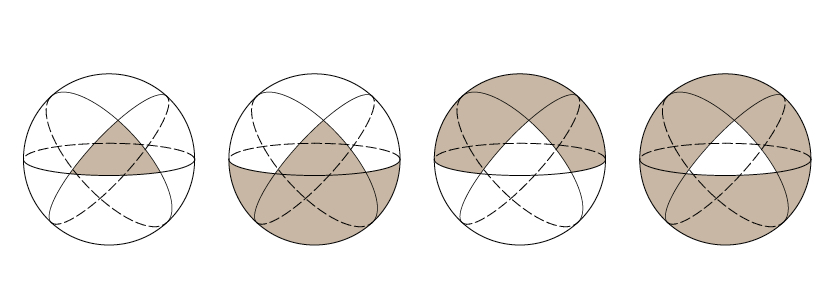
\includegraphics[width=0.9\textwidth]{kugel/Dreieckarten.jpg}
    \captionof{figure}{Dreieckarten auf einer Kugeloberfläche}
\end{center}

Der Begriff Sphärisches Dreieck oder Kugeldreieck ist ein sehr weitläufiger Begriff. 
Dabei können wir den Begriff in drei für uns wesentliche Dreiecke unterteilen:

\begin{itemize}
\item Kugelzweieck
\item Nicht Eulersche’Dreiecke
\item Eulersche’Dreiecke
\end{itemize}

\subsection{Kugelzweieck}

Zwei Grosskreise auf der Kugeloberfläche, zerlegen diese in vier gleiche Kugelzweiecke. 
Jedes dieser Dreieckseiten hat die Länge
$180^{\circ}$ oder $\pi$
Der Flächeninhalt wird dabei nur durch den Winkel $\alpha$ zwischen den beiden Grosskreisen bestimmt.

\begin{center}
        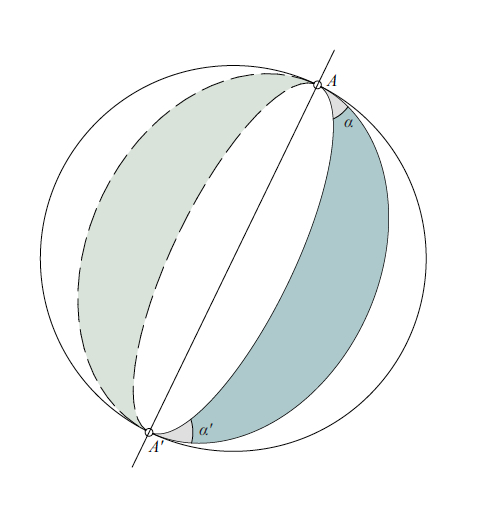
\includegraphics[width=0.3\textwidth]{kugel/Zweieck.jpg}
    \captionof{figure}{Bildung von Zweiecken durch Grosskreise}
\end{center}

Dabei ist der Flächeninhalt der ganzen Kugel:

\begin{align*}
A_{ Kugel } &= 4 \pi r^{2}
\end{align*}


Um den Flächeninhalt des betrachteten Zweieckes zu bekommen, 
müssen wir das ganze noch mit dem Kugelsegment mit dem Winkel $\alpha$ multiplizieren.

\begin{align*}
A_{ Zweieck } &= 4 \pi r^{2} \cdot \frac{ \alpha }{ 2 \pi }
\end{align*}


\subsection{Nicht Eulersche’ Dreiecke}

BLABLA

\subsection{Eulersche’ Dreiecke}

Legt man drei Grosskreise auf eine Kugeloberfläche, bilden sich dabei acht Dreiecke. 
Ein solches Dreieck heisst Eulersches’Dreieck\footnote{%
Leonard Euler (1707-1783), berühmter Schweizer Mathematiker und Physiker. 
Nicht Eulersche’Dreiecke erhält man, indem man das Äussere des Dreieckes ABC betrachtet.} 
Diese Dreiecke werden weder durch die Verlängerung ihrer Seiten durchschnitten, 
noch haben sie Dreiecksseiten welche grösser als $180^{\circ}$ sind.

\begin{center}
        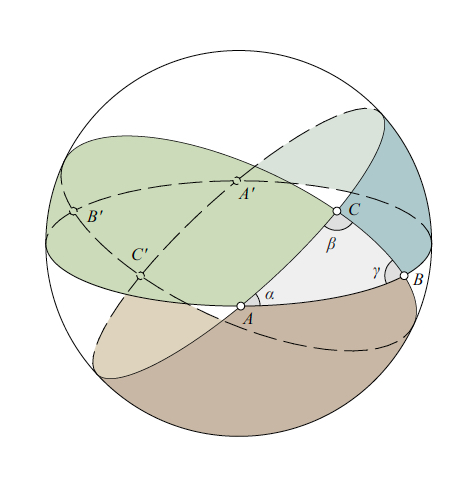
\includegraphics[width=0.4\textwidth]{kugel/Zweiecke.jpg}
    \captionof{figure}{Drei Grosskreise bilden ein sphärisches Dreieck}
\end{center}

In den nachstehenden Erklärungen und Herleitungen, sprechen wir ausschliesslich von Eulerschen’Dreiecken, da die umgeformten Winkelsätze der ebenen Trigonometrie nur auf diese Art von Kugeldreiecken angewendet werden kann.

$A_{ \overline{ ABC }}$ ist die Fläche des Dreieckes auf der Kugeloberfläche
In der ebenen Trigonometrie liegt die Winkelsumme eines Dreiecks bei
$180^{\circ}$.

Anders aber in der sphärischen Trigonometrie. Obschon sie einige Gemeinsamkeiten zur ebenen Trigonometrie aufweist, kann man nicht alles übernehmen.
So auch nicht wie Winkelsumme in einem sphärischen Dreieck.
Diese liegt bei:

\[
\begin{aligned}
\pi
&-
3\pi
&
&\text{\bigg \vert}
&
180^{\circ}
&-
540^{\circ}
\end{aligned}
\]

daraus lässt sich ableiten, das ein einzelner Winkel nicht grösser als $\pi$ oder $180^{\circ}$ sein darf. Ansonsten ist es kein Eulersches’Dreieck und wir dürfen die sphärische Trigonometrie nicht anwenden.\\
Wichtig anzumerken ist, dass die Seiten immer in Radiant beschrieben werden und nicht im Längenmass Meter wie wir es uns gewohnt sind. 
Bei den Dreiecksseiten handelt es sich um Kreisbögen und keine Strecken.

\section{Dreiecksfläche}

\begin{align*}
\text{Zweieck A}
&=
\overline{ABC} + \overline{A'BC} = 2 \alpha r^{ 2 } = A_{ \alpha }\\
\text{Zweieck B}
&=
\overline{ABC} + \overline{AB'C} = 2 \beta r^{ 2 } = A_{ \beta }\\
\text{Zweieck C}
&=
\overline{ABC} + \overline{ABC'} = 2 \gamma r^{ 2 } = A_{ \gamma }
\end{align*}

\begin{align*}
A_{ \alpha } + A_{ \beta } + A_{ \gamma } &= \frac{ 4\pi r^{ 2 } }{ 2 } + 2A_{ \overline{ ABC }} \\
2\alpha r^{ 2 } + 2\beta r^{ 2 } + 2\gamma r^{ 2 } &= \frac{ 4\pi r^{ 2 } }{ 2 } + 2A_{ \overline{ ABC }} \parallel:2\\
\alpha r^{ 2 } + \beta r^{ 2 } + \gamma r^{ 2 } &= \pi r^{ 2 } + A_{ \overline{ ABC }} \parallel-\pi r^{ 2 }\\
r^{ 2 }\left(\alpha + \beta + \gamma - \pi\right) &= A_{ \overline{ ABC }}
\end{align*}




\section{Sphärischer Exzess}
Die Winkelsumme sphärischer Dreiecke ist immer \textgreater \,  $\pi$.

\begin{align*}
\pi < \alpha + \beta + \gamma
\end{align*}

Der sphärische Exzess gibt dabei an, wie stark die Winkelsumme von $\pi$ abweicht.

\begin{align*}
\pi + \epsilon &= \alpha + \beta + \gamma \\
\epsilon &= \alpha + \beta + \gamma - \pi
\end{align*}

Würde der sphärische Exzess in der ebenen Trigonometrie angewendet, wäre dieser = 0. 
Bezieht man das auf die Erde und somit einer Kugel, kann man mit Hilfe eines beliebigen sphärischen Dreieckes und dessen Flächeninhalt auf den Radius der Kugel schliessen.

\subsection{Grenzfall - Satz von Legendre}

\begin{quote} \textit{Ein kleines sphärisches Dreieck kann näherungsweise 
wie ein ebenes Dreieck mit denselben Seiten berechnet 
werden, wenn alle Winkel des ebenen Dreiecks die um 
je ein Drittel des sphärischen Exzesses verminderten 
Winkel des sphärischen Dreiecks nimmt.} \end{quote}
\begin{flushright} - Adrien-Marie Legendre (1752-1833), Paris 1787
\end{flushright}x

Diese Aussage zeigt den Zusammenhang zwischen der 
Trigonometrie in der Ebene sowie in auf der Kugel
auf. Im speziellen bei sehr kleinen sphärischen 
Dreiecken ist die Winkelsumme nur unwesentlich 
grösser als $180^{\circ}$. Des Weiteren kann gesagt werden,
dass der sphärische Exzess gleichmässig auf alle
Winkel aufgeteilt wird.
Wichtig anzumerken ist, dass der Satz von Legendre 
für grosse, aber endliche Radien $r$ gilt.

%[SKIZZE GROSSER RADIUS/KLEINE KRÜMMUNG, KLEINER RADIUS/GROSSE KRÜMMUNG!!!!]
%


\section{Sphärisch Analoge Winkelfunktionen}

\subsection{Sphärischer Sinussatz}

Wir stellen die allgemeinen Sinussätze der Winkel $\alpha$ und $\gamma$ auf:


\[
\begin{aligned}
&{sin(\gamma)} = \frac{h}{a}
&
&\text{\bigg \vert}
&
&{sin(\alpha)} = \frac{h}{c}
&
\end{aligned}
\]

Daraus folgt:
\begin{align*}
h &= sin(\gamma)\cdot a \\
h &= sin(\alpha)\cdot c
\end{align*} 

Durch Gleichsetzung erhält man:
\begin{align*}
h &= h \\
sin(\gamma)\cdot a &= sin(\alpha)\cdot c
\end{align*} 

Durch umstellen erhalten wir den Sinussatz für a und c:
\begin{align*}
sin(\gamma)\cdot a &= sin(\alpha)\cdot c \\
\frac{sin(\gamma)}{c} &= \frac{sin(\alpha)}{a} 
\end{align*} 



\begin{align*}
\frac{sin(\alpha)}{sin(a)} = \frac{sin(\beta)}{sin(b)} = \frac{sin(\gamma)}{sin(c)}
\end{align*} 


\subsection{Winkelkosinussatz}

%[SKIZZE WINKELKOSINUS]

\[
\begin{aligned}
&\overline{C'A'} &= d\cdot {tan(b)}
&
&
&
&
&
&\overline{C'B'} &= d\cdot {tan(a)}
\end{aligned}
\]

\[
\begin{aligned}
&\overline{MA'} &= \frac{ d }{cos(b)}
&
&
&
&
&
&\overline{MB'} &= \frac{ d }{cos(a)}
\end{aligned}
\]

Der allgemeine Kosinussatz beschreibt sich wie folgt:

\begin{align*}
c^{ 2 } &= a^{ 2 } + b^{ 2 } - 2ab \cdot cos(\gamma)
\end{align*}

\begin{align*}
\triangle \overline{A'B'C' }
\overline{ A'B' }^{ 2 } &= \overline{ C'B' }^{ 2 } + \overline{ C'A' }^{ 2 } - 2 \cdot \overline{ C'B' } \cdot \overline{ C'A' } \cdot cos(\gamma)
\end{align*}



\begin{align*}
\overline{A'B'}^{ 2 } &= (d\cdot tan(a))^{ 2 } + (d\cdot tan(b))^{ 2 } - 2 \cdot (d\cdot tan(a) \cdot (d\cdot tan(b) \cdot cos(\gamma)\\
\overline{A'B'}^{ 2 } &= d^{ 2 } \cdot \left(\left(tan^{ 2 }(a) + tan^{ 2 }(b)\right) - 2\cdot tan(a) \cdot tan(b) \cdot cos(\gamma)\right)
\end{align*}

\begin{align*}
\triangle \overline{ MA'B' }
\overline{ A'B' }^{ 2 } &= \overline{ MB' }^{ 2 } + \overline{ MA' }^{ 2 } - 2\cdot \overline{ MB'} \cdot \overline{ MA' } \cdot cos(c)
\end{align*}


\begin{align*}
\overline{ A'B'}^{ 2 } &= \left(\frac{ d }{ cos(a) }  \right)^{ 2 } + \left(\frac{ d }{ cos(b)}  \right)^{ 2 } - 2 \cdot \frac{ d }{ cos(a)} \cdot \frac{ d }{ cos(b)} \cdot cos(c) \\
\overline{ A'B' }^{ 2 } &= d^{ 2 } \cdot \left(\left(\frac{ 1 }{ cos(a) }  \right)^{ 2 } + \left(\frac{ 1 }{ cos(b) }  \right)^{ 2 } - 2 \cdot \frac{ 1 }{ cos(a)} \cdot \frac{ 1 }{ cos(b)} \cdot cos(c)\right)\\
\overline{ A'B' }^{ 2 } &= d^{ 2 } \cdot \left(\left(tan^{ 2 }(a) + 1\right) + \left(tan^{ 2 }(b) + 1\right) - \left(2 \cdot \frac{cos(c)}{cos(a) \cdot cos(b)}\right)\right)
\end{align*}



\begin{align*}
\overline{ A'B'}^{ 2 } &= d^{ 2 } \cdot \left(\left(tan^{ 2 }(a) + tan^{ 2 }(b)\right) - 2 \cdot tan(a) \cdot tan(b) \cdot cos(\gamma)\right) \\
\overline{ A'B'}^{ 2 } &= d^{ 2 } \cdot \left(\left(tan^{ 2 }(a) + 1\right) + \left(tan^{ 2 }(b) + 1\right) - \left(2 \cdot \frac{cos(c)}{cos(a) \cdot cos(b)}\right)\right)
\end{align*}

Die anderen Gleichungen des Satzes, erfolgen aus Symmetriegründen.

\subsection{Seitenkosinussatz}
Durch zyklische Vertauschung des Winkelkosinus erhalten wir den Seitenkosinussatz:

\begin{align*}
{cos(a)} &= {cos(b)} \cdot {cos(c)} + {sin(b)} \cdot {sin(c)} \cdot {sin(\alpha)}\\
{cos(b)} &= {cos(a)} \cdot {cos(c)} + {sin(a)} \cdot {sin(c)} \cdot {sin(\beta)}\\
{cos(c)} &= {cos(a)} \cdot {cos(b)} + {sin(a)} \cdot {sin(b)} \cdot {sin(\gamma)}\\
\end{align*}

\section{Navigation auf See}
Das besondere an Seekarten ist die Inhaltliche Ausrichtung. Anders wie Landkarten muss sie Informationen enthalten welche für den Kapitän und seine Besatzung von grosser Bedeutung sind. Vor allem in Küstennähe ist das navigieren eines Schiffes besonders gefährlich. So enthalten Seekarten etwas über Wassertiefen, Bodenbeschaffenheiten, Gezeiten, Küstenlinien, Landzungen und Windrichtungen.
Der Hauptunterschied dabei ist, das auf der Landkarte feste Positionen definiert und aufgezeigt werden, das einzige was sich verändert ist der Reisende selbst. Bei der Seekarte ist das anders, es werden veränderliche Einwirkungen der Natur festgehalten.

Dieser kleine Unterschied zeigt die Notwendigkeit auf, die Position und den Kurs seines Schiffes auf See immer ermitteln zu können.


\section{Geographische Koordinaten}

Nachdem klar war, das die Erde eine Kugel ist, wurde diese in ein Gradnetz aufgeteilt. Dabei wurden die Angaben für eine exakte Ortsbestimmung klar definiert und die bis heute gültigen Koordinaten bestimmt.
Dabei muss man sich nochmals in Erinnerung rufen, dass sich die Erde in 24h einmal um ihre eigene Achse dreht. Nach $360 ^{\circ}$ 
und somit einer vollen Umdrehung, steht sie wieder in ihrer Ursprungsposition und ein neuer Tag beginnt.

Die Koordinaten setzen sich aus folgenden Komponenten zusammen:

\[
\begin{aligned}
&\text{Grad } (^{\circ})
&
&\text{\bigg \vert}
&
&\text{Bogenminuten } (`)
&
&\text{\bigg \vert}
&
&\text{Bogensekunden } (``)
\end{aligned}
\]

Die Erdoberfläche wurde in je 360 Breiten- und Längengrade eingeteilt. Die Breitengrade haben zueinander einen Abstand von 111.31 km, dies entspricht auch dem Abstand der Längengrade am Äquator mit Zunehmender Nähe zu den Polen, nimmt dieser Abstand ab.

\[
\begin{aligned}
&1^{\circ}
&
&\text{\bigg \vert}
&
&4 \text{ Minuten}
&
&\text{\bigg \vert}
&
&111.31\text{ km}
\end{aligned}
\]

Berechnet man nun die Erdumdrehung von 360°, erhält man genau den Erdumfang am Äquator: \begin{align*} 40’074 \text{ km.}\end{align*}

Dabei geben die Bogenminuten und -sekunden dem Standort die gewünschte Exaktheit. Mit den vollständigen Koordinaten lässt sich der Standort auf einer Landkarte exakt bestimmen und einzeichnen.

\subsection{Zeitzonen der Erde}
Wenn man nun die verschiedenen Zeitzonen der Erde betrachtet, macht die Verschiebung von jeweils einer Stunde durchaus Sinn, es lässt sich auf die Längengrade schliessen.
Zwischen den verschiedenen Zeitzonen liegen 15 Längengrade:

\begin{align*}
\text{15 Längengrade à 4 Minuten = 60 Minuten Zeitverschiebung = ca. 1665 km}
\end{align*}

Dabei ist die Zeitzone in welcher Mitte sich der Greenwich Meredian befindet die \textit{Greenwich Mean Time (GMT)} welche bis 1928 als Weltzeit galt. Im Jahr 1972 wurde diese umbenannt in die \textit{Coordinated Universal Time (UTC)} und wir von da an als Weltzeit $\pm$ 0.00 verwendet.


\section{Der Breitengrad}
Die Breitengrade bilden die bereits genannten Kleinkreise auf der Kugeloberfläche. Sie verlaufen in einem Abstand von genau 111 km parallel zum Äquator. Dabei stellt  dieser genau die Mitte zwischen Nord- und Südpol dar und teilt die Erdkugel in zwei gleiche Hälften. Somit wird von nördlicher und südlicher Breite gesprochen, je nach dem auf welcher Halbkugel man sich befindet.

%[SKIZZE DER GEOGRAFISCHEN BREITE ERDKUGEL]

\subsection{Geografische Breite $\phi$}
\begin{definition}
Die geografische Breite eines Standortes ist nichts anderes, als der Winkel am Erdmittelpunkt zwischen der Ebene des Äquators und der Geraden zum Standpunkt auf der Erdoberfläche.
\end{definition}

%[SKIZZE DER GEOGRAFISCHEN BREITE MIT WINKEL]

\subsection{Navigation mit den Breitengraden}
Da der Breitengrad bereits sehr früh ziemlich präzise bestimmt werden könnte, nutzten bereits die Seefahrer um Christoph Kolumbus den Breitengrad zur Navigation ihrer Flotten.
Den dieser lässt sich ziemlich einfach aus dem höchsten Sonnenstand oder einem Fixstern bestimmen. Dabei wird mit einem Jakobsstab\footnote{%
Der Jakobsstab ist ein früheres astronomisches Instrument zur Winkelmessung und wurde vor allem in der Seefahrt verwendet. Er ist in der Nautik der Vorläufer des Sextanten.} (später Sextant\footnote{%
Der Sextant ist ein nautisches Messinstrument zur Winkelmessung von Horizont und Fixstern (Gestirn)}) der Winkel zwischen dem Horizont und dem Fixstern gemessen. Der Winkel welchen man erhält, zieht man von 90° ab und erhält somit die geografische Breite. \\

%[SKIZZE ERMITTLUNG DES BREITENGRADES]

Wenn man sich auf der Nordhalbkugel befindet, ist der Polarstern ein sehr guter Fixstern. Befindet sich ein Schiff nun sehr nahe am Nordpol, steht dieser nahezu senkrecht am Himmelszelt bei $90^{\circ}$. Würde es aber nahe dem Äquator stehen, erscheint dieser am Horizont bei $0^{\circ}$.

\subsection{Korrekturbeiwert}

\section{Der Längengrad}
Die Längengrade bilden die bereits genannten Grosskreise auf der Kugeloberfläche.
Sie schneiden den Äquator im rechten Winkel, haben dort einen Abstand von 111 km zueinander und verbinden die Pole. Anders wie bei der geografischen Breite, ist in der Natur kein Längengrad gegeben welcher den Nullpunkt darstellt.

%[SKIZZE DER GEOGRAFISCHEN LÄNGE ERDKUGEL]

\subsection{Geografische Länge $\lambda$}
\begin{definition}
Die geografische Länge ist der Winkel an der Erdachse zum Nullmeridian.
\end{definition}

\subsection{Navigation mit den Längengraden}
Die geografische Länge lässt sich nicht so einfach bestimmen wie deren Breite. Für die Berechnung auf See benötigt man eine Referenzzeit eines Ortes mit bekannter Länge.
In der Zeit der Entdecker gab es noch keine mechanischen Uhren. Die Sonnenuhr war zudem ungeeignet, da diese nur die Uhrzeit am Standort mass und nicht die am Referenzort selbst. Die erste Pendeluhr wurde erst Mitte des 17. Jahrhunderts erfunden, was in der Schifffahrt aber auch nicht die Lösung brachte.\\
Pendeluhren auf einem Schiff sind ungeeignet, da das Pendel mit dem Wellengang aus dem Takt gebracht wird und somit die Uhr falsch geht.
Zu ungenau und gegen äussere Erschütterungen zu empfindlich waren später auch die federgetriebenen Uhren und die Unruh. Dazukamen die verschiedenen Klimazonen welche ein Schiff zu durchqueren hatten. Das Metall zog sich viel zu fest zusammen oder dehnte sich aus, was dazu führte das die Uhr unregelmässig lief.

Das sogenannte „Längenproblem“ stellte nicht nur bei der Navigation auf See ein Problem dar, es ergaben sich auch wirtschaftliche Konsequenzen. Die Schiffe mussten bis zur gewünschten geografischen Breite navigieren und segelten dann den Breitengrad entlang. Dabei waren die Schiffe oft Wochenlang unterwegs und segelten die „Breiten ab“ um an die gewünschte Position zu kommen. Dies führte zu erheblichen Zeitverlusten und viel längeren Reisezeiten.


\section{The Board of Longitude - Das Längenproblem}
Das Längenproblem beschäftigte alle grossen Seefahrernationen Europas. Wenn man bedenkt das sich Werte in einer  Höhe von halben britischen Staatshaushalten auf verloren gegangenen Schiffen befanden, erkennt man die Dringlichkeit für eine zuverlässige und genaue Navigation auf See.


\begin{itemize}
\item £ 20’000 - Abweichung von max. einem halben Grad
\item £ 15’000 - Abweichung von zwei Drittel Grad
\item £ 10’000 - Abweichung von max. $1 ^{\circ}$
\end{itemize}

\subsection{John Harrison}


\subsection{Tobias Mayer}



Uhren mit einer Abweichung von einer Minute Abweichung pro Tag (





\section{Nautische Dreieck}


$\Rightarrow$





\section{Die Vermessung der Welt}
Wir schreiben das Jahr 1818 und kehren in die Zeit des Mathematikers Carl Friedrich Gauss zurück. Neben dem liebevoll genannten „kleinen Gauss“ und anderen herausragenden Mathematischen Leistungen, beschäftigte er in den Folgejahren mit der Vermessung des Königreichs Hannovers und verfasste auf 61 Blättern das Kartenwerk \textit{Gauss’sche Landesaufnahme der 1815 durch Hannover erworbenen Gebiete}.






AUFGABE

Hubble Teleskop 
24. April 1990






\printbibliography[heading=subbibliography]
\end{refsection}




%\chapter{Geometrie auf der Kugeloberfläche\label{chapter:kugel}}
\lhead{Geometrie auf der Kugeloberfläche}
\begin{refsection}
\chapterauthor{Melina Staub und Fabian Schmid}

\section{Einleitung}

Schon seit jeher fasziniert den Menschen die Fahrt zur See. Nicht grundlos ist die Seefahrt eine der wichtigsten und ältesten Tätigkeiten der Menschheit. Der innerliche Drang neue Weltmeere und unbekannte Gebiete zu entdecken, die Fahrt zur See zu erleichtern und erträglicher zu machen, trieben die Menschen an, die Schiffe dieser Welt immer weiter zu entwickeln.

Die Idee der Kugelform der Erde ist älter als man zu denken vermag. Bereits der Schüler des antiken griechischen Philosophen Platon - Aristoteles schrieb in seiner Schrift \textit{Über den Himmel} aus dem 4. Jahrhundert v. Chr. etliche Gründe welche für die Gestallt der Erde als Kugel sprechen:

\begin{itemize}
      \item Sämtliche schweren Körper streben zum Mittelpunkt des Alls. Da sie dies von allen Seiten her gleichmäßig tun und die Erde im Mittelpunkt des Alls steht, muss sie eine kugelrunde Gestalt annehmen. 
\item Bei von der Küste wegfahrende Schiffen wird der Rumpf vor den Segeln der Sicht verborgen. 
\item In südlichen Ländern erscheinen südliche Sternbilder höher über dem Horizont.
\item Der Erdschatten bei einer Mondfinsternis ist stets rund.
\end{itemize}

Jedoch war um 1492 - der Zeit der Entdeckung Amerikas durch Christoph Kolumbus, die Idee der Erde in Kugelform noch sehr umstritten. Er erkannte anhand den Theorien und Erkenntnissen der alten Griechen, vor allem Aristoteles, das die Erde eine Kugel sein muss. \\
Doch mit seinem Vorschlag einen Seeweg über den Atlantik nach Indien zu finden und nicht wie üblich um Afrika zu segeln, stiess er beim beim portugiesischen König auf taube Ohren. Sein Plan Indien über eine Route nach Westen zu erreichen, widersprach dem gesunden Menschenverstand. Wäre die Erde wirklich eine Kugel und man befände sich auf der unteren Erdhalbkugel, würde man herunterfallen.\\
Doch auch der damals übliche Glaube an die Erde in Scheibenform brachte so einige Risiken mit sich. Was würde passieren, wenn die Flotte das Ende der Scheibe erreicht hatte? Würden sie über den Erdrand hinweggleiten und in den Abgrund stürzen?\\
Erst nach viel Überzeugungsarbeit durch Kolumbus, setzte er sich am Spanischen Hof durch und segelte über die Westliche Route über den Atlantik und entdeckte schlussendlich Amerika.

Der praktische und greifbare Beweis das die Erde eine Kugel ist, lieferte rund 30 Jahre später der Portugiese Fernando Magellan. Mit seiner Weltumsegelung und seiner Ankunft in den Philippinen, bewies er definitiv das die Erde eine Kugel ist.\\

Nun wollen wir uns die Frage stellen, wie die alten Seefahrer ohne GPS und jeglichen modernen Navigationssystemen auf hoher See wussten wo sie sich befinden und was haben die Sterne mit alldem zu tun? Reisen Sie mit uns zurück in eine Zeit mit Sextant, Kompass und Sternkarten. In die Zeit der Seefahrer und Entdecker.


\section{Geometrie auf der Ebene und der Kugel}

Euklid von Alexandria beschrieb die Grundbegriffe der ebenen Geometrie mittels Punkt, Geraden, Ebene, Winkel und Dreieck. Diese Dreiecke lassen sich mithilfe der ebenen Trigonometrie beschreiben. Dabei gelten die uns bekannten trigonometrischen Winkelfunktionen:\\

\text{Sinussatz:}
\begin{align*}
\frac{ a }{ sin(\alpha) } &= \frac{ b }{sin(\beta)} = \frac{ c }{ sin(\gamma) } = \frac{abc}{2A} = 2r\\
\end{align*}

\text{Cosinussatz:}
\begin{align*}
c^{ 2 } &= a^{ 2 } + b^{ 2 } - 2ab\cdot cos(\gamma)\\
b^{ 2 } &= a^{ 2 } + c^{ 2 } - 2ab\cdot cos(\beta)\\
a^{ 2 } &= b^{ 2 } + c^{ 2 } - 2ab\cdot cos(\alpha)
\end{align*}

Um Dreiecke auf der Kugeloberfläche zu berechnen, benötigt man die sphärische Trigonometrie. Die oben beschriebenen Sätze lassen sich auf der Kugel nicht anwenden, sie werden aber als Grundlage zur Herleitung der Sätze für das Kugeldreieck benötigt.

Die nachfolgenden Seiten thematisieren die Geometrie auf der Kugeloberfläche und wie sie in der Navigation eingesetzt werden kann.


\section{Gross- und Kleinkreise}

Eine Kugeloberfläche lässt sich in zwei verschiedene Kreisarten einteilen -  Gross- und Kleinkreise. 
Wir betrachten als erstes die Grosskreise:

\begin{definition}
Ein Großkreis ist ein größtmöglicher Kreis auf einer Kugeloberfläche. Sein Mittelpunkt fällt immer mit dem Mittelpunkt der Kugel zusammen und ein Schnitt auf dem Großkreis teilt die Kugel in jedem Fall in zwei („gleich große“) Hälften.
\end{definition}

Es gibt unendlich viele Möglichkeiten, eine Kugel in zwei gleich grosse Stücke zu zerschneiden, 
daher gibt es auch unendlich viele Grosskreise. Wenn wir die Grosskreise auf einer Kugel mit diesen auf der Erde beschreiben, sprechen wir von den Längengraden aber auch der Äquator beschreibt einen Grosskreis.
Ein Elementarer Bestandteil bilden die Grosskreise in der sphärischen Trigonometrie. Mithilfe der Schnittpunkte verschiedener Grosskreise, lässt sich ein Sphärisches Dreieck bilden auf welchem sich die sphärische Trigonometrie anwenden lässt.

[GRAFIK GROSSKREISE]

\begin{definition}
Unter Kleinkreis versteht man jene Kreise auf einer Kugeloberfläche, deren Ebenen nicht den Kugelmittelpunkt enthalten.
\end{definition}

Die Kleinkreise eignen sich im Gegensatz zu den Grosskreisen \textit{nicht} für die sphärische Trigonometrie. 
Sie werden lediglich zur Bestimmung der Messgrössen, Winkelabstände oder des Höhenwinkels eines Gestirns verwendet. 

Wenn wir die Kleinkreise auf die Erdoberfläche projizieren betrachten wir die Breitengrade.

[GRAFIK KLEINKREISE]


\section{Sphärische Dreiecke / Kugeldreieck}

\begin{center}
        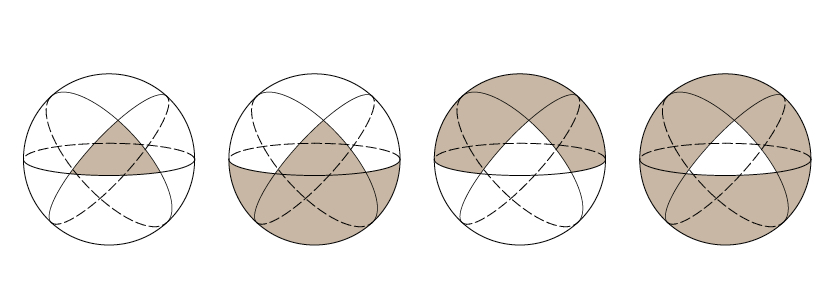
\includegraphics[width=0.9\textwidth]{kugel/Dreieckarten.jpg}
    \captionof{figure}{Dreieckarten auf einer Kugeloberfläche}
\end{center}

Der Begriff Sphärisches Dreieck oder Kugeldreieck ist ein sehr weitläufiger Begriff. 
Dabei können wir den Begriff in drei für uns wesentliche Dreiecke unterteilen:

\begin{itemize}
\item Kugelzweieck
\item Nicht Eulersche’Dreiecke
\item Eulersche’Dreiecke
\end{itemize}

\subsection{Kugelzweieck}

Zwei Grosskreise auf der Kugeloberfläche, zerlegen diese in vier gleiche Kugelzweiecke. 
Jedes dieser Dreieckseiten hat die Länge
$180^{\circ}$ oder $\pi$
Der Flächeninhalt wird dabei nur durch den Winkel $\alpha$ zwischen den beiden Grosskreisen bestimmt.

\begin{center}
        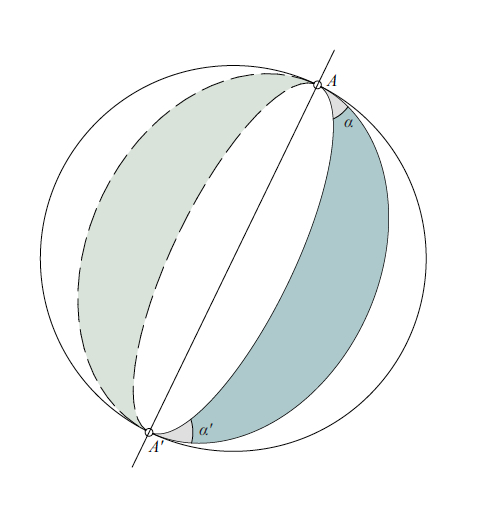
\includegraphics[width=0.3\textwidth]{kugel/Zweieck.jpg}
    \captionof{figure}{Bildung von Zweiecken durch Grosskreise}
\end{center}

Dabei ist der Flächeninhalt der ganzen Kugel:

\begin{align*}
A_{ Kugel } &= 4 \pi r^{2}
\end{align*}


Um den Flächeninhalt des betrachteten Zweieckes zu bekommen, 
müssen wir das ganze noch mit dem Kugelsegment mit dem Winkel $\alpha$ multiplizieren.

\begin{align*}
A_{ Zweieck } &= 4 \pi r^{2} \cdot \frac{ \alpha }{ 2 \pi }
\end{align*}


\subsection{Nicht Eulersche’ Dreiecke}

BLABLA

\subsection{Eulersche’ Dreiecke}

Legt man drei Grosskreise auf eine Kugeloberfläche, bilden sich dabei acht Dreiecke. 
Ein solches Dreieck heisst Eulersches’Dreieck\footnote{%
Leonard Euler (1707-1783), berühmter Schweizer Mathematiker und Physiker. 
Nicht Eulersche’Dreiecke erhält man, indem man das Äussere des Dreieckes ABC betrachtet.} 
Diese Dreiecke werden weder durch die Verlängerung ihrer Seiten durchschnitten, 
noch haben sie Dreiecksseiten welche grösser als $180^{\circ}$ sind.

\begin{center}
        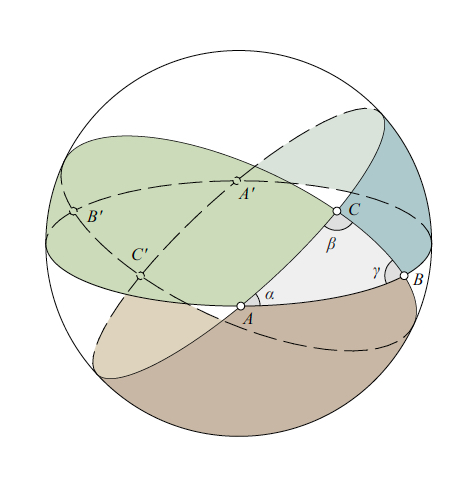
\includegraphics[width=0.4\textwidth]{kugel/Zweiecke.jpg}
    \captionof{figure}{Drei Grosskreise bilden ein sphärisches Dreieck}
\end{center}

In den nachstehenden Erklärungen und Herleitungen, sprechen wir ausschliesslich von Eulerschen’Dreiecken, da die umgeformten Winkelsätze der ebenen Trigonometrie nur auf diese Art von Kugeldreiecken angewendet werden kann.

$A_{ \overline{ ABC }}$ ist die Fläche des Dreieckes auf der Kugeloberfläche
In der ebenen Trigonometrie liegt die Winkelsumme eines Dreiecks bei
$180^{\circ}$.

Anders aber in der sphärischen Trigonometrie. Obschon sie einige Gemeinsamkeiten zur ebenen Trigonometrie aufweist, kann man nicht alles übernehmen.
So auch nicht wie Winkelsumme in einem sphärischen Dreieck.
Diese liegt bei:

\[
\begin{aligned}
\pi
&-
3\pi
&
&\text{\bigg \vert}
&
180^{\circ}
&-
540^{\circ}
\end{aligned}
\]

daraus lässt sich ableiten, das ein einzelner Winkel nicht grösser als $\pi$ oder $180^{\circ}$ sein darf. Ansonsten ist es kein Eulersches’Dreieck und wir dürfen die sphärische Trigonometrie nicht anwenden.\\
Wichtig anzumerken ist, dass die Seiten immer in Radiant beschrieben werden und nicht im Längenmass Meter wie wir es uns gewohnt sind. 
Bei den Dreiecksseiten handelt es sich um Kreisbögen und keine Strecken.

\section{Dreiecksfläche}

\begin{align*}
\text{Zweieck A}
&=
\overline{ABC} + \overline{A'BC} = 2 \alpha r^{ 2 } = A_{ \alpha }\\
\text{Zweieck B}
&=
\overline{ABC} + \overline{AB'C} = 2 \beta r^{ 2 } = A_{ \beta }\\
\text{Zweieck C}
&=
\overline{ABC} + \overline{ABC'} = 2 \gamma r^{ 2 } = A_{ \gamma }
\end{align*}

\begin{align*}
A_{ \alpha } + A_{ \beta } + A_{ \gamma } &= \frac{ 4\pi r^{ 2 } }{ 2 } + 2A_{ \overline{ ABC }} \\
2\alpha r^{ 2 } + 2\beta r^{ 2 } + 2\gamma r^{ 2 } &= \frac{ 4\pi r^{ 2 } }{ 2 } + 2A_{ \overline{ ABC }} \parallel:2\\
\alpha r^{ 2 } + \beta r^{ 2 } + \gamma r^{ 2 } &= \pi r^{ 2 } + A_{ \overline{ ABC }} \parallel-\pi r^{ 2 }\\
r^{ 2 }\left(\alpha + \beta + \gamma - \pi\right) &= A_{ \overline{ ABC }}
\end{align*}




\section{Sphärischer Exzess}
Die Winkelsumme sphärischer Dreiecke ist immer \textgreater \,  $\pi$.

\begin{align*}
\pi < \alpha + \beta + \gamma
\end{align*}

Der sphärische Exzess gibt dabei an, wie stark die Winkelsumme von $\pi$ abweicht.

\begin{align*}
\pi + \epsilon &= \alpha + \beta + \gamma \\
\epsilon &= \alpha + \beta + \gamma - \pi
\end{align*}

Würde der sphärische Exzess in der ebenen Trigonometrie angewendet, wäre dieser = 0. 
Bezieht man das auf die Erde und somit einer Kugel, kann man mit Hilfe eines beliebigen sphärischen Dreieckes und dessen Flächeninhalt auf den Radius der Kugel schliessen.

\subsection{Grenzfall - Satz von Legendre}

\begin{quote} \textit{Ein kleines sphärisches Dreieck kann näherungsweise 
wie ein ebenes Dreieck mit denselben Seiten berechnet 
werden, wenn alle Winkel des ebenen Dreiecks die um 
je ein Drittel des sphärischen Exzesses verminderten 
Winkel des sphärischen Dreiecks nimmt.} \end{quote}
\begin{flushright} - Adrien-Marie Legendre (1752-1833), Paris 1787
\end{flushright}x

Diese Aussage zeigt den Zusammenhang zwischen der 
Trigonometrie in der Ebene sowie in auf der Kugel
auf. Im speziellen bei sehr kleinen sphärischen 
Dreiecken ist die Winkelsumme nur unwesentlich 
grösser als $180^{\circ}$. Des Weiteren kann gesagt werden,
dass der sphärische Exzess gleichmässig auf alle
Winkel aufgeteilt wird.
Wichtig anzumerken ist, dass der Satz von Legendre 
für grosse, aber endliche Radien $r$ gilt.

%[SKIZZE GROSSER RADIUS/KLEINE KRÜMMUNG, KLEINER RADIUS/GROSSE KRÜMMUNG!!!!]
%


\section{Sphärisch Analoge Winkelfunktionen}

\subsection{Sphärischer Sinussatz}

Wir stellen die allgemeinen Sinussätze der Winkel $\alpha$ und $\gamma$ auf:


\[
\begin{aligned}
&{sin(\gamma)} = \frac{h}{a}
&
&\text{\bigg \vert}
&
&{sin(\alpha)} = \frac{h}{c}
&
\end{aligned}
\]

Daraus folgt:
\begin{align*}
h &= sin(\gamma)\cdot a \\
h &= sin(\alpha)\cdot c
\end{align*} 

Durch Gleichsetzung erhält man:
\begin{align*}
h &= h \\
sin(\gamma)\cdot a &= sin(\alpha)\cdot c
\end{align*} 

Durch umstellen erhalten wir den Sinussatz für a und c:
\begin{align*}
sin(\gamma)\cdot a &= sin(\alpha)\cdot c \\
\frac{sin(\gamma)}{c} &= \frac{sin(\alpha)}{a} 
\end{align*} 



\begin{align*}
\frac{sin(\alpha)}{sin(a)} = \frac{sin(\beta)}{sin(b)} = \frac{sin(\gamma)}{sin(c)}
\end{align*} 


\subsection{Winkelkosinussatz}

%[SKIZZE WINKELKOSINUS]

\[
\begin{aligned}
&\overline{C'A'} &= d\cdot {tan(b)}
&
&
&
&
&
&\overline{C'B'} &= d\cdot {tan(a)}
\end{aligned}
\]

\[
\begin{aligned}
&\overline{MA'} &= \frac{ d }{cos(b)}
&
&
&
&
&
&\overline{MB'} &= \frac{ d }{cos(a)}
\end{aligned}
\]

Der allgemeine Kosinussatz beschreibt sich wie folgt:

\begin{align*}
c^{ 2 } &= a^{ 2 } + b^{ 2 } - 2ab \cdot cos(\gamma)
\end{align*}

\begin{align*}
\triangle \overline{A'B'C' }
\overline{ A'B' }^{ 2 } &= \overline{ C'B' }^{ 2 } + \overline{ C'A' }^{ 2 } - 2 \cdot \overline{ C'B' } \cdot \overline{ C'A' } \cdot cos(\gamma)
\end{align*}



\begin{align*}
\overline{A'B'}^{ 2 } &= (d\cdot tan(a))^{ 2 } + (d\cdot tan(b))^{ 2 } - 2 \cdot (d\cdot tan(a) \cdot (d\cdot tan(b) \cdot cos(\gamma)\\
\overline{A'B'}^{ 2 } &= d^{ 2 } \cdot \left(\left(tan^{ 2 }(a) + tan^{ 2 }(b)\right) - 2\cdot tan(a) \cdot tan(b) \cdot cos(\gamma)\right)
\end{align*}

\begin{align*}
\triangle \overline{ MA'B' }
\overline{ A'B' }^{ 2 } &= \overline{ MB' }^{ 2 } + \overline{ MA' }^{ 2 } - 2\cdot \overline{ MB'} \cdot \overline{ MA' } \cdot cos(c)
\end{align*}


\begin{align*}
\overline{ A'B'}^{ 2 } &= \left(\frac{ d }{ cos(a) }  \right)^{ 2 } + \left(\frac{ d }{ cos(b)}  \right)^{ 2 } - 2 \cdot \frac{ d }{ cos(a)} \cdot \frac{ d }{ cos(b)} \cdot cos(c) \\
\overline{ A'B' }^{ 2 } &= d^{ 2 } \cdot \left(\left(\frac{ 1 }{ cos(a) }  \right)^{ 2 } + \left(\frac{ 1 }{ cos(b) }  \right)^{ 2 } - 2 \cdot \frac{ 1 }{ cos(a)} \cdot \frac{ 1 }{ cos(b)} \cdot cos(c)\right)\\
\overline{ A'B' }^{ 2 } &= d^{ 2 } \cdot \left(\left(tan^{ 2 }(a) + 1\right) + \left(tan^{ 2 }(b) + 1\right) - \left(2 \cdot \frac{cos(c)}{cos(a) \cdot cos(b)}\right)\right)
\end{align*}



\begin{align*}
\overline{ A'B'}^{ 2 } &= d^{ 2 } \cdot \left(\left(tan^{ 2 }(a) + tan^{ 2 }(b)\right) - 2 \cdot tan(a) \cdot tan(b) \cdot cos(\gamma)\right) \\
\overline{ A'B'}^{ 2 } &= d^{ 2 } \cdot \left(\left(tan^{ 2 }(a) + 1\right) + \left(tan^{ 2 }(b) + 1\right) - \left(2 \cdot \frac{cos(c)}{cos(a) \cdot cos(b)}\right)\right)
\end{align*}

Die anderen Gleichungen des Satzes, erfolgen aus Symmetriegründen.

\subsection{Seitenkosinussatz}
Durch zyklische Vertauschung des Winkelkosinus erhalten wir den Seitenkosinussatz:

\begin{align*}
{cos(a)} &= {cos(b)} \cdot {cos(c)} + {sin(b)} \cdot {sin(c)} \cdot {sin(\alpha)}\\
{cos(b)} &= {cos(a)} \cdot {cos(c)} + {sin(a)} \cdot {sin(c)} \cdot {sin(\beta)}\\
{cos(c)} &= {cos(a)} \cdot {cos(b)} + {sin(a)} \cdot {sin(b)} \cdot {sin(\gamma)}\\
\end{align*}

\section{Navigation auf See}
Das besondere an Seekarten ist die Inhaltliche Ausrichtung. Anders wie Landkarten muss sie Informationen enthalten welche für den Kapitän und seine Besatzung von grosser Bedeutung sind. Vor allem in Küstennähe ist das navigieren eines Schiffes besonders gefährlich. So enthalten Seekarten etwas über Wassertiefen, Bodenbeschaffenheiten, Gezeiten, Küstenlinien, Landzungen und Windrichtungen.
Der Hauptunterschied dabei ist, das auf der Landkarte feste Positionen definiert und aufgezeigt werden, das einzige was sich verändert ist der Reisende selbst. Bei der Seekarte ist das anders, es werden veränderliche Einwirkungen der Natur festgehalten.

Dieser kleine Unterschied zeigt die Notwendigkeit auf, die Position und den Kurs seines Schiffes auf See immer ermitteln zu können.


\section{Geographische Koordinaten}

Nachdem klar war, das die Erde eine Kugel ist, wurde diese in ein Gradnetz aufgeteilt. Dabei wurden die Angaben für eine exakte Ortsbestimmung klar definiert und die bis heute gültigen Koordinaten bestimmt.
Dabei muss man sich nochmals in Erinnerung rufen, dass sich die Erde in 24h einmal um ihre eigene Achse dreht. Nach $360 ^{\circ}$ 
und somit einer vollen Umdrehung, steht sie wieder in ihrer Ursprungsposition und ein neuer Tag beginnt.

Die Koordinaten setzen sich aus folgenden Komponenten zusammen:

\[
\begin{aligned}
&\text{Grad } (^{\circ})
&
&\text{\bigg \vert}
&
&\text{Bogenminuten } (`)
&
&\text{\bigg \vert}
&
&\text{Bogensekunden } (``)
\end{aligned}
\]

Die Erdoberfläche wurde in je 360 Breiten- und Längengrade eingeteilt. Die Breitengrade haben zueinander einen Abstand von 111.31 km, dies entspricht auch dem Abstand der Längengrade am Äquator mit Zunehmender Nähe zu den Polen, nimmt dieser Abstand ab.

\[
\begin{aligned}
&1^{\circ}
&
&\text{\bigg \vert}
&
&4 \text{ Minuten}
&
&\text{\bigg \vert}
&
&111.31\text{ km}
\end{aligned}
\]

Berechnet man nun die Erdumdrehung von 360°, erhält man genau den Erdumfang am Äquator: \begin{align*} 40’074 \text{ km.}\end{align*}

Dabei geben die Bogenminuten und -sekunden dem Standort die gewünschte Exaktheit. Mit den vollständigen Koordinaten lässt sich der Standort auf einer Landkarte exakt bestimmen und einzeichnen.

\subsection{Zeitzonen der Erde}
Wenn man nun die verschiedenen Zeitzonen der Erde betrachtet, macht die Verschiebung von jeweils einer Stunde durchaus Sinn, es lässt sich auf die Längengrade schliessen.
Zwischen den verschiedenen Zeitzonen liegen 15 Längengrade:

\begin{align*}
\text{15 Längengrade à 4 Minuten = 60 Minuten Zeitverschiebung = ca. 1665 km}
\end{align*}

Dabei ist die Zeitzone in welcher Mitte sich der Greenwich Meredian befindet die \textit{Greenwich Mean Time (GMT)} welche bis 1928 als Weltzeit galt. Im Jahr 1972 wurde diese umbenannt in die \textit{Coordinated Universal Time (UTC)} und wir von da an als Weltzeit $\pm$ 0.00 verwendet.


\section{Der Breitengrad}
Die Breitengrade bilden die bereits genannten Kleinkreise auf der Kugeloberfläche. Sie verlaufen in einem Abstand von genau 111 km parallel zum Äquator. Dabei stellt  dieser genau die Mitte zwischen Nord- und Südpol dar und teilt die Erdkugel in zwei gleiche Hälften. Somit wird von nördlicher und südlicher Breite gesprochen, je nach dem auf welcher Halbkugel man sich befindet.

%[SKIZZE DER GEOGRAFISCHEN BREITE ERDKUGEL]

\subsection{Geografische Breite $\phi$}
\begin{definition}
Die geografische Breite eines Standortes ist nichts anderes, als der Winkel am Erdmittelpunkt zwischen der Ebene des Äquators und der Geraden zum Standpunkt auf der Erdoberfläche.
\end{definition}

%[SKIZZE DER GEOGRAFISCHEN BREITE MIT WINKEL]

\subsection{Navigation mit den Breitengraden}
Da der Breitengrad bereits sehr früh ziemlich präzise bestimmt werden könnte, nutzten bereits die Seefahrer um Christoph Kolumbus den Breitengrad zur Navigation ihrer Flotten.
Den dieser lässt sich ziemlich einfach aus dem höchsten Sonnenstand oder einem Fixstern bestimmen. Dabei wird mit einem Jakobsstab\footnote{%
Der Jakobsstab ist ein früheres astronomisches Instrument zur Winkelmessung und wurde vor allem in der Seefahrt verwendet. Er ist in der Nautik der Vorläufer des Sextanten.} (später Sextant\footnote{%
Der Sextant ist ein nautisches Messinstrument zur Winkelmessung von Horizont und Fixstern (Gestirn)}) der Winkel zwischen dem Horizont und dem Fixstern gemessen. Der Winkel welchen man erhält, zieht man von 90° ab und erhält somit die geografische Breite. \\

%[SKIZZE ERMITTLUNG DES BREITENGRADES]

Wenn man sich auf der Nordhalbkugel befindet, ist der Polarstern ein sehr guter Fixstern. Befindet sich ein Schiff nun sehr nahe am Nordpol, steht dieser nahezu senkrecht am Himmelszelt bei $90^{\circ}$. Würde es aber nahe dem Äquator stehen, erscheint dieser am Horizont bei $0^{\circ}$.

\subsection{Korrekturbeiwert}

\section{Der Längengrad}
Die Längengrade bilden die bereits genannten Grosskreise auf der Kugeloberfläche.
Sie schneiden den Äquator im rechten Winkel, haben dort einen Abstand von 111 km zueinander und verbinden die Pole. Anders wie bei der geografischen Breite, ist in der Natur kein Längengrad gegeben welcher den Nullpunkt darstellt.

%[SKIZZE DER GEOGRAFISCHEN LÄNGE ERDKUGEL]

\subsection{Geografische Länge $\lambda$}
\begin{definition}
Die geografische Länge ist der Winkel an der Erdachse zum Nullmeridian.
\end{definition}

\subsection{Navigation mit den Längengraden}
Die geografische Länge lässt sich nicht so einfach bestimmen wie deren Breite. Für die Berechnung auf See benötigt man eine Referenzzeit eines Ortes mit bekannter Länge.
In der Zeit der Entdecker gab es noch keine mechanischen Uhren. Die Sonnenuhr war zudem ungeeignet, da diese nur die Uhrzeit am Standort mass und nicht die am Referenzort selbst. Die erste Pendeluhr wurde erst Mitte des 17. Jahrhunderts erfunden, was in der Schifffahrt aber auch nicht die Lösung brachte.\\
Pendeluhren auf einem Schiff sind ungeeignet, da das Pendel mit dem Wellengang aus dem Takt gebracht wird und somit die Uhr falsch geht.
Zu ungenau und gegen äussere Erschütterungen zu empfindlich waren später auch die federgetriebenen Uhren und die Unruh. Dazukamen die verschiedenen Klimazonen welche ein Schiff zu durchqueren hatten. Das Metall zog sich viel zu fest zusammen oder dehnte sich aus, was dazu führte das die Uhr unregelmässig lief.

Das sogenannte „Längenproblem“ stellte nicht nur bei der Navigation auf See ein Problem dar, es ergaben sich auch wirtschaftliche Konsequenzen. Die Schiffe mussten bis zur gewünschten geografischen Breite navigieren und segelten dann den Breitengrad entlang. Dabei waren die Schiffe oft Wochenlang unterwegs und segelten die „Breiten ab“ um an die gewünschte Position zu kommen. Dies führte zu erheblichen Zeitverlusten und viel längeren Reisezeiten.


\section{The Board of Longitude - Das Längenproblem}
Das Längenproblem beschäftigte alle grossen Seefahrernationen Europas. Wenn man bedenkt das sich Werte in einer  Höhe von halben britischen Staatshaushalten auf verloren gegangenen Schiffen befanden, erkennt man die Dringlichkeit für eine zuverlässige und genaue Navigation auf See.


\begin{itemize}
\item £ 20’000 - Abweichung von max. einem halben Grad
\item £ 15’000 - Abweichung von zwei Drittel Grad
\item £ 10’000 - Abweichung von max. $1 ^{\circ}$
\end{itemize}

\subsection{John Harrison}


\subsection{Tobias Mayer}



Uhren mit einer Abweichung von einer Minute Abweichung pro Tag (





\section{Nautische Dreieck}


$\Rightarrow$





\section{Die Vermessung der Welt}
Wir schreiben das Jahr 1818 und kehren in die Zeit des Mathematikers Carl Friedrich Gauss zurück. Neben dem liebevoll genannten „kleinen Gauss“ und anderen herausragenden Mathematischen Leistungen, beschäftigte er in den Folgejahren mit der Vermessung des Königreichs Hannovers und verfasste auf 61 Blättern das Kartenwerk \textit{Gauss’sche Landesaufnahme der 1815 durch Hannover erworbenen Gebiete}.






AUFGABE

Hubble Teleskop 
24. April 1990






\printbibliography[heading=subbibliography]
\end{refsection}




%\chapter{Geometrie auf der Kugeloberfläche\label{chapter:kugel}}
\lhead{Geometrie auf der Kugeloberfläche}
\begin{refsection}
\chapterauthor{Melina Staub und Fabian Schmid}

\section{Einleitung}

Schon seit jeher fasziniert den Menschen die Fahrt zur See. Nicht grundlos ist die Seefahrt eine der wichtigsten und ältesten Tätigkeiten der Menschheit. Der innerliche Drang neue Weltmeere und unbekannte Gebiete zu entdecken, die Fahrt zur See zu erleichtern und erträglicher zu machen, trieben die Menschen an, die Schiffe dieser Welt immer weiter zu entwickeln.

Die Idee der Kugelform der Erde ist älter als man zu denken vermag. Bereits der Schüler des antiken griechischen Philosophen Platon - Aristoteles schrieb in seiner Schrift \textit{Über den Himmel} aus dem 4. Jahrhundert v. Chr. etliche Gründe welche für die Gestallt der Erde als Kugel sprechen:

\begin{itemize}
      \item Sämtliche schweren Körper streben zum Mittelpunkt des Alls. Da sie dies von allen Seiten her gleichmäßig tun und die Erde im Mittelpunkt des Alls steht, muss sie eine kugelrunde Gestalt annehmen. 
\item Bei von der Küste wegfahrende Schiffen wird der Rumpf vor den Segeln der Sicht verborgen. 
\item In südlichen Ländern erscheinen südliche Sternbilder höher über dem Horizont.
\item Der Erdschatten bei einer Mondfinsternis ist stets rund.
\end{itemize}

Jedoch war um 1492 - der Zeit der Entdeckung Amerikas durch Christoph Kolumbus, die Idee der Erde in Kugelform noch sehr umstritten. Er erkannte anhand den Theorien und Erkenntnissen der alten Griechen, vor allem Aristoteles, das die Erde eine Kugel sein muss. \\
Doch mit seinem Vorschlag einen Seeweg über den Atlantik nach Indien zu finden und nicht wie üblich um Afrika zu segeln, stiess er beim beim portugiesischen König auf taube Ohren. Sein Plan Indien über eine Route nach Westen zu erreichen, widersprach dem gesunden Menschenverstand. Wäre die Erde wirklich eine Kugel und man befände sich auf der unteren Erdhalbkugel, würde man herunterfallen.\\
Doch auch der damals übliche Glaube an die Erde in Scheibenform brachte so einige Risiken mit sich. Was würde passieren, wenn die Flotte das Ende der Scheibe erreicht hatte? Würden sie über den Erdrand hinweggleiten und in den Abgrund stürzen?\\
Erst nach viel Überzeugungsarbeit durch Kolumbus, setzte er sich am Spanischen Hof durch und segelte über die Westliche Route über den Atlantik und entdeckte schlussendlich Amerika.

Der praktische und greifbare Beweis das die Erde eine Kugel ist, lieferte rund 30 Jahre später der Portugiese Fernando Magellan. Mit seiner Weltumsegelung und seiner Ankunft in den Philippinen, bewies er definitiv das die Erde eine Kugel ist.\\

Nun wollen wir uns die Frage stellen, wie die alten Seefahrer ohne GPS und jeglichen modernen Navigationssystemen auf hoher See wussten wo sie sich befinden und was haben die Sterne mit alldem zu tun? Reisen Sie mit uns zurück in eine Zeit mit Sextant, Kompass und Sternkarten. In die Zeit der Seefahrer und Entdecker.


\section{Geometrie auf der Ebene und der Kugel}

Euklid von Alexandria beschrieb die Grundbegriffe der ebenen Geometrie mittels Punkt, Geraden, Ebene, Winkel und Dreieck. Diese Dreiecke lassen sich mithilfe der ebenen Trigonometrie beschreiben. Dabei gelten die uns bekannten trigonometrischen Winkelfunktionen:\\

\text{Sinussatz:}
\begin{align*}
\frac{ a }{ sin(\alpha) } &= \frac{ b }{sin(\beta)} = \frac{ c }{ sin(\gamma) } = \frac{abc}{2A} = 2r\\
\end{align*}

\text{Cosinussatz:}
\begin{align*}
c^{ 2 } &= a^{ 2 } + b^{ 2 } - 2ab\cdot cos(\gamma)\\
b^{ 2 } &= a^{ 2 } + c^{ 2 } - 2ab\cdot cos(\beta)\\
a^{ 2 } &= b^{ 2 } + c^{ 2 } - 2ab\cdot cos(\alpha)
\end{align*}

Um Dreiecke auf der Kugeloberfläche zu berechnen, benötigt man die sphärische Trigonometrie. Die oben beschriebenen Sätze lassen sich auf der Kugel nicht anwenden, sie werden aber als Grundlage zur Herleitung der Sätze für das Kugeldreieck benötigt.

Die nachfolgenden Seiten thematisieren die Geometrie auf der Kugeloberfläche und wie sie in der Navigation eingesetzt werden kann.


\section{Gross- und Kleinkreise}

Eine Kugeloberfläche lässt sich in zwei verschiedene Kreisarten einteilen -  Gross- und Kleinkreise. 
Wir betrachten als erstes die Grosskreise:

\begin{definition}
Ein Großkreis ist ein größtmöglicher Kreis auf einer Kugeloberfläche. Sein Mittelpunkt fällt immer mit dem Mittelpunkt der Kugel zusammen und ein Schnitt auf dem Großkreis teilt die Kugel in jedem Fall in zwei („gleich große“) Hälften.
\end{definition}

Es gibt unendlich viele Möglichkeiten, eine Kugel in zwei gleich grosse Stücke zu zerschneiden, 
daher gibt es auch unendlich viele Grosskreise. Wenn wir die Grosskreise auf einer Kugel mit diesen auf der Erde beschreiben, sprechen wir von den Längengraden aber auch der Äquator beschreibt einen Grosskreis.
Ein Elementarer Bestandteil bilden die Grosskreise in der sphärischen Trigonometrie. Mithilfe der Schnittpunkte verschiedener Grosskreise, lässt sich ein Sphärisches Dreieck bilden auf welchem sich die sphärische Trigonometrie anwenden lässt.

[GRAFIK GROSSKREISE]

\begin{definition}
Unter Kleinkreis versteht man jene Kreise auf einer Kugeloberfläche, deren Ebenen nicht den Kugelmittelpunkt enthalten.
\end{definition}

Die Kleinkreise eignen sich im Gegensatz zu den Grosskreisen \textit{nicht} für die sphärische Trigonometrie. 
Sie werden lediglich zur Bestimmung der Messgrössen, Winkelabstände oder des Höhenwinkels eines Gestirns verwendet. 

Wenn wir die Kleinkreise auf die Erdoberfläche projizieren betrachten wir die Breitengrade.

[GRAFIK KLEINKREISE]


\section{Sphärische Dreiecke / Kugeldreieck}

\begin{center}
        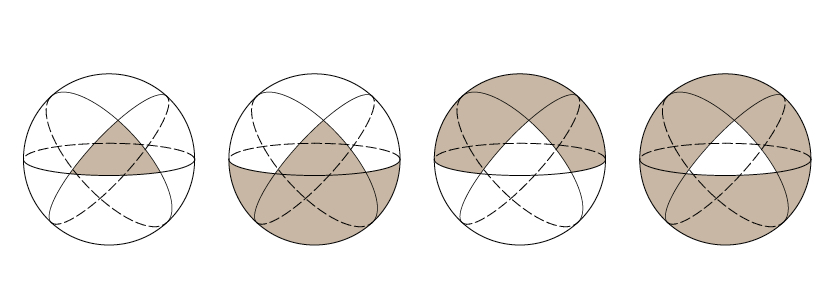
\includegraphics[width=0.9\textwidth]{kugel/Dreieckarten.jpg}
    \captionof{figure}{Dreieckarten auf einer Kugeloberfläche}
\end{center}

Der Begriff Sphärisches Dreieck oder Kugeldreieck ist ein sehr weitläufiger Begriff. 
Dabei können wir den Begriff in drei für uns wesentliche Dreiecke unterteilen:

\begin{itemize}
\item Kugelzweieck
\item Nicht Eulersche’Dreiecke
\item Eulersche’Dreiecke
\end{itemize}

\subsection{Kugelzweieck}

Zwei Grosskreise auf der Kugeloberfläche, zerlegen diese in vier gleiche Kugelzweiecke. 
Jedes dieser Dreieckseiten hat die Länge
$180^{\circ}$ oder $\pi$
Der Flächeninhalt wird dabei nur durch den Winkel $\alpha$ zwischen den beiden Grosskreisen bestimmt.

\begin{center}
        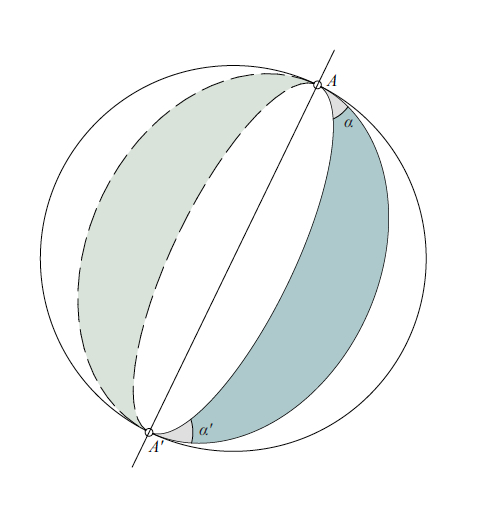
\includegraphics[width=0.3\textwidth]{kugel/Zweieck.jpg}
    \captionof{figure}{Bildung von Zweiecken durch Grosskreise}
\end{center}

Dabei ist der Flächeninhalt der ganzen Kugel:

\begin{align*}
A_{ Kugel } &= 4 \pi r^{2}
\end{align*}


Um den Flächeninhalt des betrachteten Zweieckes zu bekommen, 
müssen wir das ganze noch mit dem Kugelsegment mit dem Winkel $\alpha$ multiplizieren.

\begin{align*}
A_{ Zweieck } &= 4 \pi r^{2} \cdot \frac{ \alpha }{ 2 \pi }
\end{align*}


\subsection{Nicht Eulersche’ Dreiecke}

BLABLA

\subsection{Eulersche’ Dreiecke}

Legt man drei Grosskreise auf eine Kugeloberfläche, bilden sich dabei acht Dreiecke. 
Ein solches Dreieck heisst Eulersches’Dreieck\footnote{%
Leonard Euler (1707-1783), berühmter Schweizer Mathematiker und Physiker. 
Nicht Eulersche’Dreiecke erhält man, indem man das Äussere des Dreieckes ABC betrachtet.} 
Diese Dreiecke werden weder durch die Verlängerung ihrer Seiten durchschnitten, 
noch haben sie Dreiecksseiten welche grösser als $180^{\circ}$ sind.

\begin{center}
        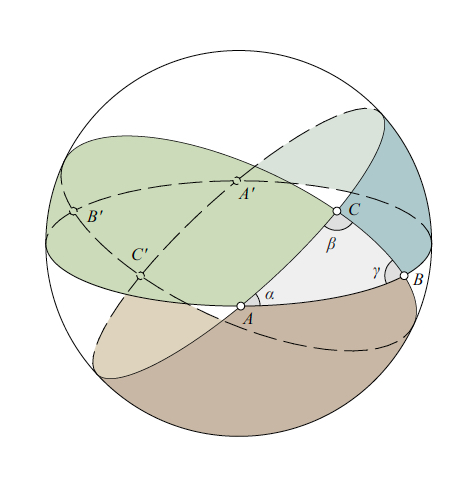
\includegraphics[width=0.4\textwidth]{kugel/Zweiecke.jpg}
    \captionof{figure}{Drei Grosskreise bilden ein sphärisches Dreieck}
\end{center}

In den nachstehenden Erklärungen und Herleitungen, sprechen wir ausschliesslich von Eulerschen’Dreiecken, da die umgeformten Winkelsätze der ebenen Trigonometrie nur auf diese Art von Kugeldreiecken angewendet werden kann.

$A_{ \overline{ ABC }}$ ist die Fläche des Dreieckes auf der Kugeloberfläche
In der ebenen Trigonometrie liegt die Winkelsumme eines Dreiecks bei
$180^{\circ}$.

Anders aber in der sphärischen Trigonometrie. Obschon sie einige Gemeinsamkeiten zur ebenen Trigonometrie aufweist, kann man nicht alles übernehmen.
So auch nicht wie Winkelsumme in einem sphärischen Dreieck.
Diese liegt bei:

\[
\begin{aligned}
\pi
&-
3\pi
&
&\text{\bigg \vert}
&
180^{\circ}
&-
540^{\circ}
\end{aligned}
\]

daraus lässt sich ableiten, das ein einzelner Winkel nicht grösser als $\pi$ oder $180^{\circ}$ sein darf. Ansonsten ist es kein Eulersches’Dreieck und wir dürfen die sphärische Trigonometrie nicht anwenden.\\
Wichtig anzumerken ist, dass die Seiten immer in Radiant beschrieben werden und nicht im Längenmass Meter wie wir es uns gewohnt sind. 
Bei den Dreiecksseiten handelt es sich um Kreisbögen und keine Strecken.

\section{Dreiecksfläche}

\begin{align*}
\text{Zweieck A}
&=
\overline{ABC} + \overline{A'BC} = 2 \alpha r^{ 2 } = A_{ \alpha }\\
\text{Zweieck B}
&=
\overline{ABC} + \overline{AB'C} = 2 \beta r^{ 2 } = A_{ \beta }\\
\text{Zweieck C}
&=
\overline{ABC} + \overline{ABC'} = 2 \gamma r^{ 2 } = A_{ \gamma }
\end{align*}

\begin{align*}
A_{ \alpha } + A_{ \beta } + A_{ \gamma } &= \frac{ 4\pi r^{ 2 } }{ 2 } + 2A_{ \overline{ ABC }} \\
2\alpha r^{ 2 } + 2\beta r^{ 2 } + 2\gamma r^{ 2 } &= \frac{ 4\pi r^{ 2 } }{ 2 } + 2A_{ \overline{ ABC }} \parallel:2\\
\alpha r^{ 2 } + \beta r^{ 2 } + \gamma r^{ 2 } &= \pi r^{ 2 } + A_{ \overline{ ABC }} \parallel-\pi r^{ 2 }\\
r^{ 2 }\left(\alpha + \beta + \gamma - \pi\right) &= A_{ \overline{ ABC }}
\end{align*}




\section{Sphärischer Exzess}
Die Winkelsumme sphärischer Dreiecke ist immer \textgreater \,  $\pi$.

\begin{align*}
\pi < \alpha + \beta + \gamma
\end{align*}

Der sphärische Exzess gibt dabei an, wie stark die Winkelsumme von $\pi$ abweicht.

\begin{align*}
\pi + \epsilon &= \alpha + \beta + \gamma \\
\epsilon &= \alpha + \beta + \gamma - \pi
\end{align*}

Würde der sphärische Exzess in der ebenen Trigonometrie angewendet, wäre dieser = 0. 
Bezieht man das auf die Erde und somit einer Kugel, kann man mit Hilfe eines beliebigen sphärischen Dreieckes und dessen Flächeninhalt auf den Radius der Kugel schliessen.

\subsection{Grenzfall - Satz von Legendre}

\begin{quote} \textit{Ein kleines sphärisches Dreieck kann näherungsweise 
wie ein ebenes Dreieck mit denselben Seiten berechnet 
werden, wenn alle Winkel des ebenen Dreiecks die um 
je ein Drittel des sphärischen Exzesses verminderten 
Winkel des sphärischen Dreiecks nimmt.} \end{quote}
\begin{flushright} - Adrien-Marie Legendre (1752-1833), Paris 1787
\end{flushright}x

Diese Aussage zeigt den Zusammenhang zwischen der 
Trigonometrie in der Ebene sowie in auf der Kugel
auf. Im speziellen bei sehr kleinen sphärischen 
Dreiecken ist die Winkelsumme nur unwesentlich 
grösser als $180^{\circ}$. Des Weiteren kann gesagt werden,
dass der sphärische Exzess gleichmässig auf alle
Winkel aufgeteilt wird.
Wichtig anzumerken ist, dass der Satz von Legendre 
für grosse, aber endliche Radien $r$ gilt.

%[SKIZZE GROSSER RADIUS/KLEINE KRÜMMUNG, KLEINER RADIUS/GROSSE KRÜMMUNG!!!!]
%


\section{Sphärisch Analoge Winkelfunktionen}

\subsection{Sphärischer Sinussatz}

Wir stellen die allgemeinen Sinussätze der Winkel $\alpha$ und $\gamma$ auf:


\[
\begin{aligned}
&{sin(\gamma)} = \frac{h}{a}
&
&\text{\bigg \vert}
&
&{sin(\alpha)} = \frac{h}{c}
&
\end{aligned}
\]

Daraus folgt:
\begin{align*}
h &= sin(\gamma)\cdot a \\
h &= sin(\alpha)\cdot c
\end{align*} 

Durch Gleichsetzung erhält man:
\begin{align*}
h &= h \\
sin(\gamma)\cdot a &= sin(\alpha)\cdot c
\end{align*} 

Durch umstellen erhalten wir den Sinussatz für a und c:
\begin{align*}
sin(\gamma)\cdot a &= sin(\alpha)\cdot c \\
\frac{sin(\gamma)}{c} &= \frac{sin(\alpha)}{a} 
\end{align*} 



\begin{align*}
\frac{sin(\alpha)}{sin(a)} = \frac{sin(\beta)}{sin(b)} = \frac{sin(\gamma)}{sin(c)}
\end{align*} 


\subsection{Winkelkosinussatz}

%[SKIZZE WINKELKOSINUS]

\[
\begin{aligned}
&\overline{C'A'} &= d\cdot {tan(b)}
&
&
&
&
&
&\overline{C'B'} &= d\cdot {tan(a)}
\end{aligned}
\]

\[
\begin{aligned}
&\overline{MA'} &= \frac{ d }{cos(b)}
&
&
&
&
&
&\overline{MB'} &= \frac{ d }{cos(a)}
\end{aligned}
\]

Der allgemeine Kosinussatz beschreibt sich wie folgt:

\begin{align*}
c^{ 2 } &= a^{ 2 } + b^{ 2 } - 2ab \cdot cos(\gamma)
\end{align*}

\begin{align*}
\triangle \overline{A'B'C' }
\overline{ A'B' }^{ 2 } &= \overline{ C'B' }^{ 2 } + \overline{ C'A' }^{ 2 } - 2 \cdot \overline{ C'B' } \cdot \overline{ C'A' } \cdot cos(\gamma)
\end{align*}



\begin{align*}
\overline{A'B'}^{ 2 } &= (d\cdot tan(a))^{ 2 } + (d\cdot tan(b))^{ 2 } - 2 \cdot (d\cdot tan(a) \cdot (d\cdot tan(b) \cdot cos(\gamma)\\
\overline{A'B'}^{ 2 } &= d^{ 2 } \cdot \left(\left(tan^{ 2 }(a) + tan^{ 2 }(b)\right) - 2\cdot tan(a) \cdot tan(b) \cdot cos(\gamma)\right)
\end{align*}

\begin{align*}
\triangle \overline{ MA'B' }
\overline{ A'B' }^{ 2 } &= \overline{ MB' }^{ 2 } + \overline{ MA' }^{ 2 } - 2\cdot \overline{ MB'} \cdot \overline{ MA' } \cdot cos(c)
\end{align*}


\begin{align*}
\overline{ A'B'}^{ 2 } &= \left(\frac{ d }{ cos(a) }  \right)^{ 2 } + \left(\frac{ d }{ cos(b)}  \right)^{ 2 } - 2 \cdot \frac{ d }{ cos(a)} \cdot \frac{ d }{ cos(b)} \cdot cos(c) \\
\overline{ A'B' }^{ 2 } &= d^{ 2 } \cdot \left(\left(\frac{ 1 }{ cos(a) }  \right)^{ 2 } + \left(\frac{ 1 }{ cos(b) }  \right)^{ 2 } - 2 \cdot \frac{ 1 }{ cos(a)} \cdot \frac{ 1 }{ cos(b)} \cdot cos(c)\right)\\
\overline{ A'B' }^{ 2 } &= d^{ 2 } \cdot \left(\left(tan^{ 2 }(a) + 1\right) + \left(tan^{ 2 }(b) + 1\right) - \left(2 \cdot \frac{cos(c)}{cos(a) \cdot cos(b)}\right)\right)
\end{align*}



\begin{align*}
\overline{ A'B'}^{ 2 } &= d^{ 2 } \cdot \left(\left(tan^{ 2 }(a) + tan^{ 2 }(b)\right) - 2 \cdot tan(a) \cdot tan(b) \cdot cos(\gamma)\right) \\
\overline{ A'B'}^{ 2 } &= d^{ 2 } \cdot \left(\left(tan^{ 2 }(a) + 1\right) + \left(tan^{ 2 }(b) + 1\right) - \left(2 \cdot \frac{cos(c)}{cos(a) \cdot cos(b)}\right)\right)
\end{align*}

Die anderen Gleichungen des Satzes, erfolgen aus Symmetriegründen.

\subsection{Seitenkosinussatz}
Durch zyklische Vertauschung des Winkelkosinus erhalten wir den Seitenkosinussatz:

\begin{align*}
{cos(a)} &= {cos(b)} \cdot {cos(c)} + {sin(b)} \cdot {sin(c)} \cdot {sin(\alpha)}\\
{cos(b)} &= {cos(a)} \cdot {cos(c)} + {sin(a)} \cdot {sin(c)} \cdot {sin(\beta)}\\
{cos(c)} &= {cos(a)} \cdot {cos(b)} + {sin(a)} \cdot {sin(b)} \cdot {sin(\gamma)}\\
\end{align*}

\section{Navigation auf See}
Das besondere an Seekarten ist die Inhaltliche Ausrichtung. Anders wie Landkarten muss sie Informationen enthalten welche für den Kapitän und seine Besatzung von grosser Bedeutung sind. Vor allem in Küstennähe ist das navigieren eines Schiffes besonders gefährlich. So enthalten Seekarten etwas über Wassertiefen, Bodenbeschaffenheiten, Gezeiten, Küstenlinien, Landzungen und Windrichtungen.
Der Hauptunterschied dabei ist, das auf der Landkarte feste Positionen definiert und aufgezeigt werden, das einzige was sich verändert ist der Reisende selbst. Bei der Seekarte ist das anders, es werden veränderliche Einwirkungen der Natur festgehalten.

Dieser kleine Unterschied zeigt die Notwendigkeit auf, die Position und den Kurs seines Schiffes auf See immer ermitteln zu können.


\section{Geographische Koordinaten}

Nachdem klar war, das die Erde eine Kugel ist, wurde diese in ein Gradnetz aufgeteilt. Dabei wurden die Angaben für eine exakte Ortsbestimmung klar definiert und die bis heute gültigen Koordinaten bestimmt.
Dabei muss man sich nochmals in Erinnerung rufen, dass sich die Erde in 24h einmal um ihre eigene Achse dreht. Nach $360 ^{\circ}$ 
und somit einer vollen Umdrehung, steht sie wieder in ihrer Ursprungsposition und ein neuer Tag beginnt.

Die Koordinaten setzen sich aus folgenden Komponenten zusammen:

\[
\begin{aligned}
&\text{Grad } (^{\circ})
&
&\text{\bigg \vert}
&
&\text{Bogenminuten } (`)
&
&\text{\bigg \vert}
&
&\text{Bogensekunden } (``)
\end{aligned}
\]

Die Erdoberfläche wurde in je 360 Breiten- und Längengrade eingeteilt. Die Breitengrade haben zueinander einen Abstand von 111.31 km, dies entspricht auch dem Abstand der Längengrade am Äquator mit Zunehmender Nähe zu den Polen, nimmt dieser Abstand ab.

\[
\begin{aligned}
&1^{\circ}
&
&\text{\bigg \vert}
&
&4 \text{ Minuten}
&
&\text{\bigg \vert}
&
&111.31\text{ km}
\end{aligned}
\]

Berechnet man nun die Erdumdrehung von 360°, erhält man genau den Erdumfang am Äquator: \begin{align*} 40’074 \text{ km.}\end{align*}

Dabei geben die Bogenminuten und -sekunden dem Standort die gewünschte Exaktheit. Mit den vollständigen Koordinaten lässt sich der Standort auf einer Landkarte exakt bestimmen und einzeichnen.

\subsection{Zeitzonen der Erde}
Wenn man nun die verschiedenen Zeitzonen der Erde betrachtet, macht die Verschiebung von jeweils einer Stunde durchaus Sinn, es lässt sich auf die Längengrade schliessen.
Zwischen den verschiedenen Zeitzonen liegen 15 Längengrade:

\begin{align*}
\text{15 Längengrade à 4 Minuten = 60 Minuten Zeitverschiebung = ca. 1665 km}
\end{align*}

Dabei ist die Zeitzone in welcher Mitte sich der Greenwich Meredian befindet die \textit{Greenwich Mean Time (GMT)} welche bis 1928 als Weltzeit galt. Im Jahr 1972 wurde diese umbenannt in die \textit{Coordinated Universal Time (UTC)} und wir von da an als Weltzeit $\pm$ 0.00 verwendet.


\section{Der Breitengrad}
Die Breitengrade bilden die bereits genannten Kleinkreise auf der Kugeloberfläche. Sie verlaufen in einem Abstand von genau 111 km parallel zum Äquator. Dabei stellt  dieser genau die Mitte zwischen Nord- und Südpol dar und teilt die Erdkugel in zwei gleiche Hälften. Somit wird von nördlicher und südlicher Breite gesprochen, je nach dem auf welcher Halbkugel man sich befindet.

%[SKIZZE DER GEOGRAFISCHEN BREITE ERDKUGEL]

\subsection{Geografische Breite $\phi$}
\begin{definition}
Die geografische Breite eines Standortes ist nichts anderes, als der Winkel am Erdmittelpunkt zwischen der Ebene des Äquators und der Geraden zum Standpunkt auf der Erdoberfläche.
\end{definition}

%[SKIZZE DER GEOGRAFISCHEN BREITE MIT WINKEL]

\subsection{Navigation mit den Breitengraden}
Da der Breitengrad bereits sehr früh ziemlich präzise bestimmt werden könnte, nutzten bereits die Seefahrer um Christoph Kolumbus den Breitengrad zur Navigation ihrer Flotten.
Den dieser lässt sich ziemlich einfach aus dem höchsten Sonnenstand oder einem Fixstern bestimmen. Dabei wird mit einem Jakobsstab\footnote{%
Der Jakobsstab ist ein früheres astronomisches Instrument zur Winkelmessung und wurde vor allem in der Seefahrt verwendet. Er ist in der Nautik der Vorläufer des Sextanten.} (später Sextant\footnote{%
Der Sextant ist ein nautisches Messinstrument zur Winkelmessung von Horizont und Fixstern (Gestirn)}) der Winkel zwischen dem Horizont und dem Fixstern gemessen. Der Winkel welchen man erhält, zieht man von 90° ab und erhält somit die geografische Breite. \\

%[SKIZZE ERMITTLUNG DES BREITENGRADES]

Wenn man sich auf der Nordhalbkugel befindet, ist der Polarstern ein sehr guter Fixstern. Befindet sich ein Schiff nun sehr nahe am Nordpol, steht dieser nahezu senkrecht am Himmelszelt bei $90^{\circ}$. Würde es aber nahe dem Äquator stehen, erscheint dieser am Horizont bei $0^{\circ}$.

\subsection{Korrekturbeiwert}

\section{Der Längengrad}
Die Längengrade bilden die bereits genannten Grosskreise auf der Kugeloberfläche.
Sie schneiden den Äquator im rechten Winkel, haben dort einen Abstand von 111 km zueinander und verbinden die Pole. Anders wie bei der geografischen Breite, ist in der Natur kein Längengrad gegeben welcher den Nullpunkt darstellt.

%[SKIZZE DER GEOGRAFISCHEN LÄNGE ERDKUGEL]

\subsection{Geografische Länge $\lambda$}
\begin{definition}
Die geografische Länge ist der Winkel an der Erdachse zum Nullmeridian.
\end{definition}

\subsection{Navigation mit den Längengraden}
Die geografische Länge lässt sich nicht so einfach bestimmen wie deren Breite. Für die Berechnung auf See benötigt man eine Referenzzeit eines Ortes mit bekannter Länge.
In der Zeit der Entdecker gab es noch keine mechanischen Uhren. Die Sonnenuhr war zudem ungeeignet, da diese nur die Uhrzeit am Standort mass und nicht die am Referenzort selbst. Die erste Pendeluhr wurde erst Mitte des 17. Jahrhunderts erfunden, was in der Schifffahrt aber auch nicht die Lösung brachte.\\
Pendeluhren auf einem Schiff sind ungeeignet, da das Pendel mit dem Wellengang aus dem Takt gebracht wird und somit die Uhr falsch geht.
Zu ungenau und gegen äussere Erschütterungen zu empfindlich waren später auch die federgetriebenen Uhren und die Unruh. Dazukamen die verschiedenen Klimazonen welche ein Schiff zu durchqueren hatten. Das Metall zog sich viel zu fest zusammen oder dehnte sich aus, was dazu führte das die Uhr unregelmässig lief.

Das sogenannte „Längenproblem“ stellte nicht nur bei der Navigation auf See ein Problem dar, es ergaben sich auch wirtschaftliche Konsequenzen. Die Schiffe mussten bis zur gewünschten geografischen Breite navigieren und segelten dann den Breitengrad entlang. Dabei waren die Schiffe oft Wochenlang unterwegs und segelten die „Breiten ab“ um an die gewünschte Position zu kommen. Dies führte zu erheblichen Zeitverlusten und viel längeren Reisezeiten.


\section{The Board of Longitude - Das Längenproblem}
Das Längenproblem beschäftigte alle grossen Seefahrernationen Europas. Wenn man bedenkt das sich Werte in einer  Höhe von halben britischen Staatshaushalten auf verloren gegangenen Schiffen befanden, erkennt man die Dringlichkeit für eine zuverlässige und genaue Navigation auf See.


\begin{itemize}
\item £ 20’000 - Abweichung von max. einem halben Grad
\item £ 15’000 - Abweichung von zwei Drittel Grad
\item £ 10’000 - Abweichung von max. $1 ^{\circ}$
\end{itemize}

\subsection{John Harrison}


\subsection{Tobias Mayer}



Uhren mit einer Abweichung von einer Minute Abweichung pro Tag (





\section{Nautische Dreieck}


$\Rightarrow$





\section{Die Vermessung der Welt}
Wir schreiben das Jahr 1818 und kehren in die Zeit des Mathematikers Carl Friedrich Gauss zurück. Neben dem liebevoll genannten „kleinen Gauss“ und anderen herausragenden Mathematischen Leistungen, beschäftigte er in den Folgejahren mit der Vermessung des Königreichs Hannovers und verfasste auf 61 Blättern das Kartenwerk \textit{Gauss’sche Landesaufnahme der 1815 durch Hannover erworbenen Gebiete}.






AUFGABE

Hubble Teleskop 
24. April 1990






\printbibliography[heading=subbibliography]
\end{refsection}




%\chapter{Geometrie auf der Kugeloberfläche\label{chapter:kugel}}
\lhead{Geometrie auf der Kugeloberfläche}
\begin{refsection}
\chapterauthor{Melina Staub und Fabian Schmid}

\section{Einleitung}

Schon seit jeher fasziniert den Menschen die Fahrt zur See. Nicht grundlos ist die Seefahrt eine der wichtigsten und ältesten Tätigkeiten der Menschheit. Der innerliche Drang neue Weltmeere und unbekannte Gebiete zu entdecken, die Fahrt zur See zu erleichtern und erträglicher zu machen, trieben die Menschen an, die Schiffe dieser Welt immer weiter zu entwickeln.

Die Idee der Kugelform der Erde ist älter als man zu denken vermag. Bereits der Schüler des antiken griechischen Philosophen Platon - Aristoteles schrieb in seiner Schrift \textit{Über den Himmel} aus dem 4. Jahrhundert v. Chr. etliche Gründe welche für die Gestallt der Erde als Kugel sprechen:

\begin{itemize}
      \item Sämtliche schweren Körper streben zum Mittelpunkt des Alls. Da sie dies von allen Seiten her gleichmäßig tun und die Erde im Mittelpunkt des Alls steht, muss sie eine kugelrunde Gestalt annehmen. 
\item Bei von der Küste wegfahrende Schiffen wird der Rumpf vor den Segeln der Sicht verborgen. 
\item In südlichen Ländern erscheinen südliche Sternbilder höher über dem Horizont.
\item Der Erdschatten bei einer Mondfinsternis ist stets rund.
\end{itemize}

Jedoch war um 1492 - der Zeit der Entdeckung Amerikas durch Christoph Kolumbus, die Idee der Erde in Kugelform noch sehr umstritten. Er erkannte anhand den Theorien und Erkenntnissen der alten Griechen, vor allem Aristoteles, das die Erde eine Kugel sein muss. \\
Doch mit seinem Vorschlag einen Seeweg über den Atlantik nach Indien zu finden und nicht wie üblich um Afrika zu segeln, stiess er beim beim portugiesischen König auf taube Ohren. Sein Plan Indien über eine Route nach Westen zu erreichen, widersprach dem gesunden Menschenverstand. Wäre die Erde wirklich eine Kugel und man befände sich auf der unteren Erdhalbkugel, würde man herunterfallen.\\
Doch auch der damals übliche Glaube an die Erde in Scheibenform brachte so einige Risiken mit sich. Was würde passieren, wenn die Flotte das Ende der Scheibe erreicht hatte? Würden sie über den Erdrand hinweggleiten und in den Abgrund stürzen?\\
Erst nach viel Überzeugungsarbeit durch Kolumbus, setzte er sich am Spanischen Hof durch und segelte über die Westliche Route über den Atlantik und entdeckte schlussendlich Amerika.

Der praktische und greifbare Beweis das die Erde eine Kugel ist, lieferte rund 30 Jahre später der Portugiese Fernando Magellan. Mit seiner Weltumsegelung und seiner Ankunft in den Philippinen, bewies er definitiv das die Erde eine Kugel ist.\\

Nun wollen wir uns die Frage stellen, wie die alten Seefahrer ohne GPS und jeglichen modernen Navigationssystemen auf hoher See wussten wo sie sich befinden und was haben die Sterne mit alldem zu tun? Reisen Sie mit uns zurück in eine Zeit mit Sextant, Kompass und Sternkarten. In die Zeit der Seefahrer und Entdecker.


\section{Geometrie auf der Ebene und der Kugel}

Euklid von Alexandria beschrieb die Grundbegriffe der ebenen Geometrie mittels Punkt, Geraden, Ebene, Winkel und Dreieck. Diese Dreiecke lassen sich mithilfe der ebenen Trigonometrie beschreiben. Dabei gelten die uns bekannten trigonometrischen Winkelfunktionen:\\

\text{Sinussatz:}
\begin{align*}
\frac{ a }{ sin(\alpha) } &= \frac{ b }{sin(\beta)} = \frac{ c }{ sin(\gamma) } = \frac{abc}{2A} = 2r\\
\end{align*}

\text{Cosinussatz:}
\begin{align*}
c^{ 2 } &= a^{ 2 } + b^{ 2 } - 2ab\cdot cos(\gamma)\\
b^{ 2 } &= a^{ 2 } + c^{ 2 } - 2ab\cdot cos(\beta)\\
a^{ 2 } &= b^{ 2 } + c^{ 2 } - 2ab\cdot cos(\alpha)
\end{align*}

Um Dreiecke auf der Kugeloberfläche zu berechnen, benötigt man die sphärische Trigonometrie. Die oben beschriebenen Sätze lassen sich auf der Kugel nicht anwenden, sie werden aber als Grundlage zur Herleitung der Sätze für das Kugeldreieck benötigt.

Die nachfolgenden Seiten thematisieren die Geometrie auf der Kugeloberfläche und wie sie in der Navigation eingesetzt werden kann.


\section{Gross- und Kleinkreise}

Eine Kugeloberfläche lässt sich in zwei verschiedene Kreisarten einteilen -  Gross- und Kleinkreise. 
Wir betrachten als erstes die Grosskreise:

\begin{definition}
Ein Großkreis ist ein größtmöglicher Kreis auf einer Kugeloberfläche. Sein Mittelpunkt fällt immer mit dem Mittelpunkt der Kugel zusammen und ein Schnitt auf dem Großkreis teilt die Kugel in jedem Fall in zwei („gleich große“) Hälften.
\end{definition}

Es gibt unendlich viele Möglichkeiten, eine Kugel in zwei gleich grosse Stücke zu zerschneiden, 
daher gibt es auch unendlich viele Grosskreise. Wenn wir die Grosskreise auf einer Kugel mit diesen auf der Erde beschreiben, sprechen wir von den Längengraden aber auch der Äquator beschreibt einen Grosskreis.
Ein Elementarer Bestandteil bilden die Grosskreise in der sphärischen Trigonometrie. Mithilfe der Schnittpunkte verschiedener Grosskreise, lässt sich ein Sphärisches Dreieck bilden auf welchem sich die sphärische Trigonometrie anwenden lässt.

[GRAFIK GROSSKREISE]

\begin{definition}
Unter Kleinkreis versteht man jene Kreise auf einer Kugeloberfläche, deren Ebenen nicht den Kugelmittelpunkt enthalten.
\end{definition}

Die Kleinkreise eignen sich im Gegensatz zu den Grosskreisen \textit{nicht} für die sphärische Trigonometrie. 
Sie werden lediglich zur Bestimmung der Messgrössen, Winkelabstände oder des Höhenwinkels eines Gestirns verwendet. 

Wenn wir die Kleinkreise auf die Erdoberfläche projizieren betrachten wir die Breitengrade.

[GRAFIK KLEINKREISE]


\section{Sphärische Dreiecke / Kugeldreieck}

\begin{center}
        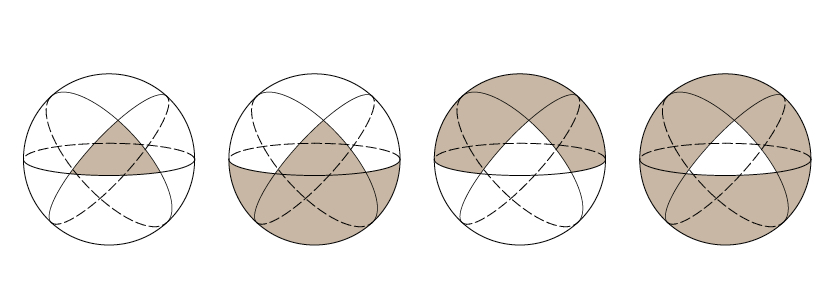
\includegraphics[width=0.9\textwidth]{kugel/Dreieckarten.jpg}
    \captionof{figure}{Dreieckarten auf einer Kugeloberfläche}
\end{center}

Der Begriff Sphärisches Dreieck oder Kugeldreieck ist ein sehr weitläufiger Begriff. 
Dabei können wir den Begriff in drei für uns wesentliche Dreiecke unterteilen:

\begin{itemize}
\item Kugelzweieck
\item Nicht Eulersche’Dreiecke
\item Eulersche’Dreiecke
\end{itemize}

\subsection{Kugelzweieck}

Zwei Grosskreise auf der Kugeloberfläche, zerlegen diese in vier gleiche Kugelzweiecke. 
Jedes dieser Dreieckseiten hat die Länge
$180^{\circ}$ oder $\pi$
Der Flächeninhalt wird dabei nur durch den Winkel $\alpha$ zwischen den beiden Grosskreisen bestimmt.

\begin{center}
        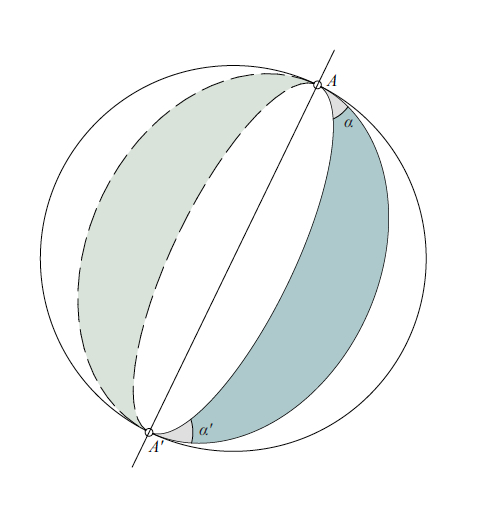
\includegraphics[width=0.3\textwidth]{kugel/Zweieck.jpg}
    \captionof{figure}{Bildung von Zweiecken durch Grosskreise}
\end{center}

Dabei ist der Flächeninhalt der ganzen Kugel:

\begin{align*}
A_{ Kugel } &= 4 \pi r^{2}
\end{align*}


Um den Flächeninhalt des betrachteten Zweieckes zu bekommen, 
müssen wir das ganze noch mit dem Kugelsegment mit dem Winkel $\alpha$ multiplizieren.

\begin{align*}
A_{ Zweieck } &= 4 \pi r^{2} \cdot \frac{ \alpha }{ 2 \pi }
\end{align*}


\subsection{Nicht Eulersche’ Dreiecke}

BLABLA

\subsection{Eulersche’ Dreiecke}

Legt man drei Grosskreise auf eine Kugeloberfläche, bilden sich dabei acht Dreiecke. 
Ein solches Dreieck heisst Eulersches’Dreieck\footnote{%
Leonard Euler (1707-1783), berühmter Schweizer Mathematiker und Physiker. 
Nicht Eulersche’Dreiecke erhält man, indem man das Äussere des Dreieckes ABC betrachtet.} 
Diese Dreiecke werden weder durch die Verlängerung ihrer Seiten durchschnitten, 
noch haben sie Dreiecksseiten welche grösser als $180^{\circ}$ sind.

\begin{center}
        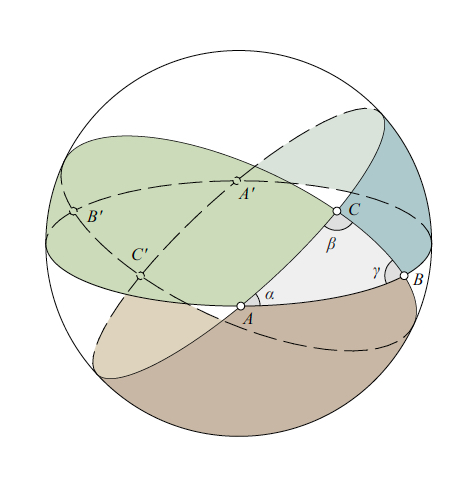
\includegraphics[width=0.4\textwidth]{kugel/Zweiecke.jpg}
    \captionof{figure}{Drei Grosskreise bilden ein sphärisches Dreieck}
\end{center}

In den nachstehenden Erklärungen und Herleitungen, sprechen wir ausschliesslich von Eulerschen’Dreiecken, da die umgeformten Winkelsätze der ebenen Trigonometrie nur auf diese Art von Kugeldreiecken angewendet werden kann.

$A_{ \overline{ ABC }}$ ist die Fläche des Dreieckes auf der Kugeloberfläche
In der ebenen Trigonometrie liegt die Winkelsumme eines Dreiecks bei
$180^{\circ}$.

Anders aber in der sphärischen Trigonometrie. Obschon sie einige Gemeinsamkeiten zur ebenen Trigonometrie aufweist, kann man nicht alles übernehmen.
So auch nicht wie Winkelsumme in einem sphärischen Dreieck.
Diese liegt bei:

\[
\begin{aligned}
\pi
&-
3\pi
&
&\text{\bigg \vert}
&
180^{\circ}
&-
540^{\circ}
\end{aligned}
\]

daraus lässt sich ableiten, das ein einzelner Winkel nicht grösser als $\pi$ oder $180^{\circ}$ sein darf. Ansonsten ist es kein Eulersches’Dreieck und wir dürfen die sphärische Trigonometrie nicht anwenden.\\
Wichtig anzumerken ist, dass die Seiten immer in Radiant beschrieben werden und nicht im Längenmass Meter wie wir es uns gewohnt sind. 
Bei den Dreiecksseiten handelt es sich um Kreisbögen und keine Strecken.

\section{Dreiecksfläche}

\begin{align*}
\text{Zweieck A}
&=
\overline{ABC} + \overline{A'BC} = 2 \alpha r^{ 2 } = A_{ \alpha }\\
\text{Zweieck B}
&=
\overline{ABC} + \overline{AB'C} = 2 \beta r^{ 2 } = A_{ \beta }\\
\text{Zweieck C}
&=
\overline{ABC} + \overline{ABC'} = 2 \gamma r^{ 2 } = A_{ \gamma }
\end{align*}

\begin{align*}
A_{ \alpha } + A_{ \beta } + A_{ \gamma } &= \frac{ 4\pi r^{ 2 } }{ 2 } + 2A_{ \overline{ ABC }} \\
2\alpha r^{ 2 } + 2\beta r^{ 2 } + 2\gamma r^{ 2 } &= \frac{ 4\pi r^{ 2 } }{ 2 } + 2A_{ \overline{ ABC }} \parallel:2\\
\alpha r^{ 2 } + \beta r^{ 2 } + \gamma r^{ 2 } &= \pi r^{ 2 } + A_{ \overline{ ABC }} \parallel-\pi r^{ 2 }\\
r^{ 2 }\left(\alpha + \beta + \gamma - \pi\right) &= A_{ \overline{ ABC }}
\end{align*}




\section{Sphärischer Exzess}
Die Winkelsumme sphärischer Dreiecke ist immer \textgreater \,  $\pi$.

\begin{align*}
\pi < \alpha + \beta + \gamma
\end{align*}

Der sphärische Exzess gibt dabei an, wie stark die Winkelsumme von $\pi$ abweicht.

\begin{align*}
\pi + \epsilon &= \alpha + \beta + \gamma \\
\epsilon &= \alpha + \beta + \gamma - \pi
\end{align*}

Würde der sphärische Exzess in der ebenen Trigonometrie angewendet, wäre dieser = 0. 
Bezieht man das auf die Erde und somit einer Kugel, kann man mit Hilfe eines beliebigen sphärischen Dreieckes und dessen Flächeninhalt auf den Radius der Kugel schliessen.

\subsection{Grenzfall - Satz von Legendre}

\begin{quote} \textit{Ein kleines sphärisches Dreieck kann näherungsweise 
wie ein ebenes Dreieck mit denselben Seiten berechnet 
werden, wenn alle Winkel des ebenen Dreiecks die um 
je ein Drittel des sphärischen Exzesses verminderten 
Winkel des sphärischen Dreiecks nimmt.} \end{quote}
\begin{flushright} - Adrien-Marie Legendre (1752-1833), Paris 1787
\end{flushright}x

Diese Aussage zeigt den Zusammenhang zwischen der 
Trigonometrie in der Ebene sowie in auf der Kugel
auf. Im speziellen bei sehr kleinen sphärischen 
Dreiecken ist die Winkelsumme nur unwesentlich 
grösser als $180^{\circ}$. Des Weiteren kann gesagt werden,
dass der sphärische Exzess gleichmässig auf alle
Winkel aufgeteilt wird.
Wichtig anzumerken ist, dass der Satz von Legendre 
für grosse, aber endliche Radien $r$ gilt.

%[SKIZZE GROSSER RADIUS/KLEINE KRÜMMUNG, KLEINER RADIUS/GROSSE KRÜMMUNG!!!!]
%


\section{Sphärisch Analoge Winkelfunktionen}

\subsection{Sphärischer Sinussatz}

Wir stellen die allgemeinen Sinussätze der Winkel $\alpha$ und $\gamma$ auf:


\[
\begin{aligned}
&{sin(\gamma)} = \frac{h}{a}
&
&\text{\bigg \vert}
&
&{sin(\alpha)} = \frac{h}{c}
&
\end{aligned}
\]

Daraus folgt:
\begin{align*}
h &= sin(\gamma)\cdot a \\
h &= sin(\alpha)\cdot c
\end{align*} 

Durch Gleichsetzung erhält man:
\begin{align*}
h &= h \\
sin(\gamma)\cdot a &= sin(\alpha)\cdot c
\end{align*} 

Durch umstellen erhalten wir den Sinussatz für a und c:
\begin{align*}
sin(\gamma)\cdot a &= sin(\alpha)\cdot c \\
\frac{sin(\gamma)}{c} &= \frac{sin(\alpha)}{a} 
\end{align*} 



\begin{align*}
\frac{sin(\alpha)}{sin(a)} = \frac{sin(\beta)}{sin(b)} = \frac{sin(\gamma)}{sin(c)}
\end{align*} 


\subsection{Winkelkosinussatz}

%[SKIZZE WINKELKOSINUS]

\[
\begin{aligned}
&\overline{C'A'} &= d\cdot {tan(b)}
&
&
&
&
&
&\overline{C'B'} &= d\cdot {tan(a)}
\end{aligned}
\]

\[
\begin{aligned}
&\overline{MA'} &= \frac{ d }{cos(b)}
&
&
&
&
&
&\overline{MB'} &= \frac{ d }{cos(a)}
\end{aligned}
\]

Der allgemeine Kosinussatz beschreibt sich wie folgt:

\begin{align*}
c^{ 2 } &= a^{ 2 } + b^{ 2 } - 2ab \cdot cos(\gamma)
\end{align*}

\begin{align*}
\triangle \overline{A'B'C' }
\overline{ A'B' }^{ 2 } &= \overline{ C'B' }^{ 2 } + \overline{ C'A' }^{ 2 } - 2 \cdot \overline{ C'B' } \cdot \overline{ C'A' } \cdot cos(\gamma)
\end{align*}



\begin{align*}
\overline{A'B'}^{ 2 } &= (d\cdot tan(a))^{ 2 } + (d\cdot tan(b))^{ 2 } - 2 \cdot (d\cdot tan(a) \cdot (d\cdot tan(b) \cdot cos(\gamma)\\
\overline{A'B'}^{ 2 } &= d^{ 2 } \cdot \left(\left(tan^{ 2 }(a) + tan^{ 2 }(b)\right) - 2\cdot tan(a) \cdot tan(b) \cdot cos(\gamma)\right)
\end{align*}

\begin{align*}
\triangle \overline{ MA'B' }
\overline{ A'B' }^{ 2 } &= \overline{ MB' }^{ 2 } + \overline{ MA' }^{ 2 } - 2\cdot \overline{ MB'} \cdot \overline{ MA' } \cdot cos(c)
\end{align*}


\begin{align*}
\overline{ A'B'}^{ 2 } &= \left(\frac{ d }{ cos(a) }  \right)^{ 2 } + \left(\frac{ d }{ cos(b)}  \right)^{ 2 } - 2 \cdot \frac{ d }{ cos(a)} \cdot \frac{ d }{ cos(b)} \cdot cos(c) \\
\overline{ A'B' }^{ 2 } &= d^{ 2 } \cdot \left(\left(\frac{ 1 }{ cos(a) }  \right)^{ 2 } + \left(\frac{ 1 }{ cos(b) }  \right)^{ 2 } - 2 \cdot \frac{ 1 }{ cos(a)} \cdot \frac{ 1 }{ cos(b)} \cdot cos(c)\right)\\
\overline{ A'B' }^{ 2 } &= d^{ 2 } \cdot \left(\left(tan^{ 2 }(a) + 1\right) + \left(tan^{ 2 }(b) + 1\right) - \left(2 \cdot \frac{cos(c)}{cos(a) \cdot cos(b)}\right)\right)
\end{align*}



\begin{align*}
\overline{ A'B'}^{ 2 } &= d^{ 2 } \cdot \left(\left(tan^{ 2 }(a) + tan^{ 2 }(b)\right) - 2 \cdot tan(a) \cdot tan(b) \cdot cos(\gamma)\right) \\
\overline{ A'B'}^{ 2 } &= d^{ 2 } \cdot \left(\left(tan^{ 2 }(a) + 1\right) + \left(tan^{ 2 }(b) + 1\right) - \left(2 \cdot \frac{cos(c)}{cos(a) \cdot cos(b)}\right)\right)
\end{align*}

Die anderen Gleichungen des Satzes, erfolgen aus Symmetriegründen.

\subsection{Seitenkosinussatz}
Durch zyklische Vertauschung des Winkelkosinus erhalten wir den Seitenkosinussatz:

\begin{align*}
{cos(a)} &= {cos(b)} \cdot {cos(c)} + {sin(b)} \cdot {sin(c)} \cdot {sin(\alpha)}\\
{cos(b)} &= {cos(a)} \cdot {cos(c)} + {sin(a)} \cdot {sin(c)} \cdot {sin(\beta)}\\
{cos(c)} &= {cos(a)} \cdot {cos(b)} + {sin(a)} \cdot {sin(b)} \cdot {sin(\gamma)}\\
\end{align*}

\section{Navigation auf See}
Das besondere an Seekarten ist die Inhaltliche Ausrichtung. Anders wie Landkarten muss sie Informationen enthalten welche für den Kapitän und seine Besatzung von grosser Bedeutung sind. Vor allem in Küstennähe ist das navigieren eines Schiffes besonders gefährlich. So enthalten Seekarten etwas über Wassertiefen, Bodenbeschaffenheiten, Gezeiten, Küstenlinien, Landzungen und Windrichtungen.
Der Hauptunterschied dabei ist, das auf der Landkarte feste Positionen definiert und aufgezeigt werden, das einzige was sich verändert ist der Reisende selbst. Bei der Seekarte ist das anders, es werden veränderliche Einwirkungen der Natur festgehalten.

Dieser kleine Unterschied zeigt die Notwendigkeit auf, die Position und den Kurs seines Schiffes auf See immer ermitteln zu können.


\section{Geographische Koordinaten}

Nachdem klar war, das die Erde eine Kugel ist, wurde diese in ein Gradnetz aufgeteilt. Dabei wurden die Angaben für eine exakte Ortsbestimmung klar definiert und die bis heute gültigen Koordinaten bestimmt.
Dabei muss man sich nochmals in Erinnerung rufen, dass sich die Erde in 24h einmal um ihre eigene Achse dreht. Nach $360 ^{\circ}$ 
und somit einer vollen Umdrehung, steht sie wieder in ihrer Ursprungsposition und ein neuer Tag beginnt.

Die Koordinaten setzen sich aus folgenden Komponenten zusammen:

\[
\begin{aligned}
&\text{Grad } (^{\circ})
&
&\text{\bigg \vert}
&
&\text{Bogenminuten } (`)
&
&\text{\bigg \vert}
&
&\text{Bogensekunden } (``)
\end{aligned}
\]

Die Erdoberfläche wurde in je 360 Breiten- und Längengrade eingeteilt. Die Breitengrade haben zueinander einen Abstand von 111.31 km, dies entspricht auch dem Abstand der Längengrade am Äquator mit Zunehmender Nähe zu den Polen, nimmt dieser Abstand ab.

\[
\begin{aligned}
&1^{\circ}
&
&\text{\bigg \vert}
&
&4 \text{ Minuten}
&
&\text{\bigg \vert}
&
&111.31\text{ km}
\end{aligned}
\]

Berechnet man nun die Erdumdrehung von 360°, erhält man genau den Erdumfang am Äquator: \begin{align*} 40’074 \text{ km.}\end{align*}

Dabei geben die Bogenminuten und -sekunden dem Standort die gewünschte Exaktheit. Mit den vollständigen Koordinaten lässt sich der Standort auf einer Landkarte exakt bestimmen und einzeichnen.

\subsection{Zeitzonen der Erde}
Wenn man nun die verschiedenen Zeitzonen der Erde betrachtet, macht die Verschiebung von jeweils einer Stunde durchaus Sinn, es lässt sich auf die Längengrade schliessen.
Zwischen den verschiedenen Zeitzonen liegen 15 Längengrade:

\begin{align*}
\text{15 Längengrade à 4 Minuten = 60 Minuten Zeitverschiebung = ca. 1665 km}
\end{align*}

Dabei ist die Zeitzone in welcher Mitte sich der Greenwich Meredian befindet die \textit{Greenwich Mean Time (GMT)} welche bis 1928 als Weltzeit galt. Im Jahr 1972 wurde diese umbenannt in die \textit{Coordinated Universal Time (UTC)} und wir von da an als Weltzeit $\pm$ 0.00 verwendet.


\section{Der Breitengrad}
Die Breitengrade bilden die bereits genannten Kleinkreise auf der Kugeloberfläche. Sie verlaufen in einem Abstand von genau 111 km parallel zum Äquator. Dabei stellt  dieser genau die Mitte zwischen Nord- und Südpol dar und teilt die Erdkugel in zwei gleiche Hälften. Somit wird von nördlicher und südlicher Breite gesprochen, je nach dem auf welcher Halbkugel man sich befindet.

%[SKIZZE DER GEOGRAFISCHEN BREITE ERDKUGEL]

\subsection{Geografische Breite $\phi$}
\begin{definition}
Die geografische Breite eines Standortes ist nichts anderes, als der Winkel am Erdmittelpunkt zwischen der Ebene des Äquators und der Geraden zum Standpunkt auf der Erdoberfläche.
\end{definition}

%[SKIZZE DER GEOGRAFISCHEN BREITE MIT WINKEL]

\subsection{Navigation mit den Breitengraden}
Da der Breitengrad bereits sehr früh ziemlich präzise bestimmt werden könnte, nutzten bereits die Seefahrer um Christoph Kolumbus den Breitengrad zur Navigation ihrer Flotten.
Den dieser lässt sich ziemlich einfach aus dem höchsten Sonnenstand oder einem Fixstern bestimmen. Dabei wird mit einem Jakobsstab\footnote{%
Der Jakobsstab ist ein früheres astronomisches Instrument zur Winkelmessung und wurde vor allem in der Seefahrt verwendet. Er ist in der Nautik der Vorläufer des Sextanten.} (später Sextant\footnote{%
Der Sextant ist ein nautisches Messinstrument zur Winkelmessung von Horizont und Fixstern (Gestirn)}) der Winkel zwischen dem Horizont und dem Fixstern gemessen. Der Winkel welchen man erhält, zieht man von 90° ab und erhält somit die geografische Breite. \\

%[SKIZZE ERMITTLUNG DES BREITENGRADES]

Wenn man sich auf der Nordhalbkugel befindet, ist der Polarstern ein sehr guter Fixstern. Befindet sich ein Schiff nun sehr nahe am Nordpol, steht dieser nahezu senkrecht am Himmelszelt bei $90^{\circ}$. Würde es aber nahe dem Äquator stehen, erscheint dieser am Horizont bei $0^{\circ}$.

\subsection{Korrekturbeiwert}

\section{Der Längengrad}
Die Längengrade bilden die bereits genannten Grosskreise auf der Kugeloberfläche.
Sie schneiden den Äquator im rechten Winkel, haben dort einen Abstand von 111 km zueinander und verbinden die Pole. Anders wie bei der geografischen Breite, ist in der Natur kein Längengrad gegeben welcher den Nullpunkt darstellt.

%[SKIZZE DER GEOGRAFISCHEN LÄNGE ERDKUGEL]

\subsection{Geografische Länge $\lambda$}
\begin{definition}
Die geografische Länge ist der Winkel an der Erdachse zum Nullmeridian.
\end{definition}

\subsection{Navigation mit den Längengraden}
Die geografische Länge lässt sich nicht so einfach bestimmen wie deren Breite. Für die Berechnung auf See benötigt man eine Referenzzeit eines Ortes mit bekannter Länge.
In der Zeit der Entdecker gab es noch keine mechanischen Uhren. Die Sonnenuhr war zudem ungeeignet, da diese nur die Uhrzeit am Standort mass und nicht die am Referenzort selbst. Die erste Pendeluhr wurde erst Mitte des 17. Jahrhunderts erfunden, was in der Schifffahrt aber auch nicht die Lösung brachte.\\
Pendeluhren auf einem Schiff sind ungeeignet, da das Pendel mit dem Wellengang aus dem Takt gebracht wird und somit die Uhr falsch geht.
Zu ungenau und gegen äussere Erschütterungen zu empfindlich waren später auch die federgetriebenen Uhren und die Unruh. Dazukamen die verschiedenen Klimazonen welche ein Schiff zu durchqueren hatten. Das Metall zog sich viel zu fest zusammen oder dehnte sich aus, was dazu führte das die Uhr unregelmässig lief.

Das sogenannte „Längenproblem“ stellte nicht nur bei der Navigation auf See ein Problem dar, es ergaben sich auch wirtschaftliche Konsequenzen. Die Schiffe mussten bis zur gewünschten geografischen Breite navigieren und segelten dann den Breitengrad entlang. Dabei waren die Schiffe oft Wochenlang unterwegs und segelten die „Breiten ab“ um an die gewünschte Position zu kommen. Dies führte zu erheblichen Zeitverlusten und viel längeren Reisezeiten.


\section{The Board of Longitude - Das Längenproblem}
Das Längenproblem beschäftigte alle grossen Seefahrernationen Europas. Wenn man bedenkt das sich Werte in einer  Höhe von halben britischen Staatshaushalten auf verloren gegangenen Schiffen befanden, erkennt man die Dringlichkeit für eine zuverlässige und genaue Navigation auf See.


\begin{itemize}
\item £ 20’000 - Abweichung von max. einem halben Grad
\item £ 15’000 - Abweichung von zwei Drittel Grad
\item £ 10’000 - Abweichung von max. $1 ^{\circ}$
\end{itemize}

\subsection{John Harrison}


\subsection{Tobias Mayer}



Uhren mit einer Abweichung von einer Minute Abweichung pro Tag (





\section{Nautische Dreieck}


$\Rightarrow$





\section{Die Vermessung der Welt}
Wir schreiben das Jahr 1818 und kehren in die Zeit des Mathematikers Carl Friedrich Gauss zurück. Neben dem liebevoll genannten „kleinen Gauss“ und anderen herausragenden Mathematischen Leistungen, beschäftigte er in den Folgejahren mit der Vermessung des Königreichs Hannovers und verfasste auf 61 Blättern das Kartenwerk \textit{Gauss’sche Landesaufnahme der 1815 durch Hannover erworbenen Gebiete}.






AUFGABE

Hubble Teleskop 
24. April 1990






\printbibliography[heading=subbibliography]
\end{refsection}




%\chapter{Geometrie auf der Kugeloberfläche\label{chapter:kugel}}
\lhead{Geometrie auf der Kugeloberfläche}
\begin{refsection}
\chapterauthor{Melina Staub und Fabian Schmid}

\section{Einleitung}

Schon seit jeher fasziniert den Menschen die Fahrt zur See. Nicht grundlos ist die Seefahrt eine der wichtigsten und ältesten Tätigkeiten der Menschheit. Der innerliche Drang neue Weltmeere und unbekannte Gebiete zu entdecken, die Fahrt zur See zu erleichtern und erträglicher zu machen, trieben die Menschen an, die Schiffe dieser Welt immer weiter zu entwickeln.

Die Idee der Kugelform der Erde ist älter als man zu denken vermag. Bereits der Schüler des antiken griechischen Philosophen Platon - Aristoteles schrieb in seiner Schrift \textit{Über den Himmel} aus dem 4. Jahrhundert v. Chr. etliche Gründe welche für die Gestallt der Erde als Kugel sprechen:

\begin{itemize}
      \item Sämtliche schweren Körper streben zum Mittelpunkt des Alls. Da sie dies von allen Seiten her gleichmäßig tun und die Erde im Mittelpunkt des Alls steht, muss sie eine kugelrunde Gestalt annehmen. 
\item Bei von der Küste wegfahrende Schiffen wird der Rumpf vor den Segeln der Sicht verborgen. 
\item In südlichen Ländern erscheinen südliche Sternbilder höher über dem Horizont.
\item Der Erdschatten bei einer Mondfinsternis ist stets rund.
\end{itemize}

Jedoch war um 1492 - der Zeit der Entdeckung Amerikas durch Christoph Kolumbus, die Idee der Erde in Kugelform noch sehr umstritten. Er erkannte anhand den Theorien und Erkenntnissen der alten Griechen, vor allem Aristoteles, das die Erde eine Kugel sein muss. \\
Doch mit seinem Vorschlag einen Seeweg über den Atlantik nach Indien zu finden und nicht wie üblich um Afrika zu segeln, stiess er beim beim portugiesischen König auf taube Ohren. Sein Plan Indien über eine Route nach Westen zu erreichen, widersprach dem gesunden Menschenverstand. Wäre die Erde wirklich eine Kugel und man befände sich auf der unteren Erdhalbkugel, würde man herunterfallen.\\
Doch auch der damals übliche Glaube an die Erde in Scheibenform brachte so einige Risiken mit sich. Was würde passieren, wenn die Flotte das Ende der Scheibe erreicht hatte? Würden sie über den Erdrand hinweggleiten und in den Abgrund stürzen?\\
Erst nach viel Überzeugungsarbeit durch Kolumbus, setzte er sich am Spanischen Hof durch und segelte über die Westliche Route über den Atlantik und entdeckte schlussendlich Amerika.

Der praktische und greifbare Beweis das die Erde eine Kugel ist, lieferte rund 30 Jahre später der Portugiese Fernando Magellan. Mit seiner Weltumsegelung und seiner Ankunft in den Philippinen, bewies er definitiv das die Erde eine Kugel ist.\\

Nun wollen wir uns die Frage stellen, wie die alten Seefahrer ohne GPS und jeglichen modernen Navigationssystemen auf hoher See wussten wo sie sich befinden und was haben die Sterne mit alldem zu tun? Reisen Sie mit uns zurück in eine Zeit mit Sextant, Kompass und Sternkarten. In die Zeit der Seefahrer und Entdecker.


\section{Geometrie auf der Ebene und der Kugel}

Euklid von Alexandria beschrieb die Grundbegriffe der ebenen Geometrie mittels Punkt, Geraden, Ebene, Winkel und Dreieck. Diese Dreiecke lassen sich mithilfe der ebenen Trigonometrie beschreiben. Dabei gelten die uns bekannten trigonometrischen Winkelfunktionen:\\

\text{Sinussatz:}
\begin{align*}
\frac{ a }{ sin(\alpha) } &= \frac{ b }{sin(\beta)} = \frac{ c }{ sin(\gamma) } = \frac{abc}{2A} = 2r\\
\end{align*}

\text{Cosinussatz:}
\begin{align*}
c^{ 2 } &= a^{ 2 } + b^{ 2 } - 2ab\cdot cos(\gamma)\\
b^{ 2 } &= a^{ 2 } + c^{ 2 } - 2ab\cdot cos(\beta)\\
a^{ 2 } &= b^{ 2 } + c^{ 2 } - 2ab\cdot cos(\alpha)
\end{align*}

Um Dreiecke auf der Kugeloberfläche zu berechnen, benötigt man die sphärische Trigonometrie. Die oben beschriebenen Sätze lassen sich auf der Kugel nicht anwenden, sie werden aber als Grundlage zur Herleitung der Sätze für das Kugeldreieck benötigt.

Die nachfolgenden Seiten thematisieren die Geometrie auf der Kugeloberfläche und wie sie in der Navigation eingesetzt werden kann.


\section{Gross- und Kleinkreise}

Eine Kugeloberfläche lässt sich in zwei verschiedene Kreisarten einteilen -  Gross- und Kleinkreise. 
Wir betrachten als erstes die Grosskreise:

\begin{definition}
Ein Großkreis ist ein größtmöglicher Kreis auf einer Kugeloberfläche. Sein Mittelpunkt fällt immer mit dem Mittelpunkt der Kugel zusammen und ein Schnitt auf dem Großkreis teilt die Kugel in jedem Fall in zwei („gleich große“) Hälften.
\end{definition}

Es gibt unendlich viele Möglichkeiten, eine Kugel in zwei gleich grosse Stücke zu zerschneiden, 
daher gibt es auch unendlich viele Grosskreise. Wenn wir die Grosskreise auf einer Kugel mit diesen auf der Erde beschreiben, sprechen wir von den Längengraden aber auch der Äquator beschreibt einen Grosskreis.
Ein Elementarer Bestandteil bilden die Grosskreise in der sphärischen Trigonometrie. Mithilfe der Schnittpunkte verschiedener Grosskreise, lässt sich ein Sphärisches Dreieck bilden auf welchem sich die sphärische Trigonometrie anwenden lässt.

[GRAFIK GROSSKREISE]

\begin{definition}
Unter Kleinkreis versteht man jene Kreise auf einer Kugeloberfläche, deren Ebenen nicht den Kugelmittelpunkt enthalten.
\end{definition}

Die Kleinkreise eignen sich im Gegensatz zu den Grosskreisen \textit{nicht} für die sphärische Trigonometrie. 
Sie werden lediglich zur Bestimmung der Messgrössen, Winkelabstände oder des Höhenwinkels eines Gestirns verwendet. 

Wenn wir die Kleinkreise auf die Erdoberfläche projizieren betrachten wir die Breitengrade.

[GRAFIK KLEINKREISE]


\section{Sphärische Dreiecke / Kugeldreieck}

\begin{center}
        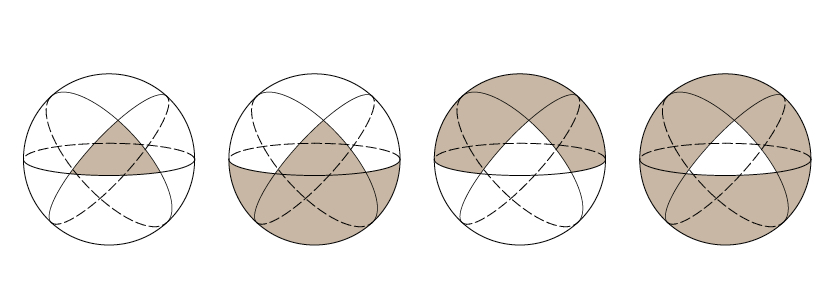
\includegraphics[width=0.9\textwidth]{kugel/Dreieckarten.jpg}
    \captionof{figure}{Dreieckarten auf einer Kugeloberfläche}
\end{center}

Der Begriff Sphärisches Dreieck oder Kugeldreieck ist ein sehr weitläufiger Begriff. 
Dabei können wir den Begriff in drei für uns wesentliche Dreiecke unterteilen:

\begin{itemize}
\item Kugelzweieck
\item Nicht Eulersche’Dreiecke
\item Eulersche’Dreiecke
\end{itemize}

\subsection{Kugelzweieck}

Zwei Grosskreise auf der Kugeloberfläche, zerlegen diese in vier gleiche Kugelzweiecke. 
Jedes dieser Dreieckseiten hat die Länge
$180^{\circ}$ oder $\pi$
Der Flächeninhalt wird dabei nur durch den Winkel $\alpha$ zwischen den beiden Grosskreisen bestimmt.

\begin{center}
        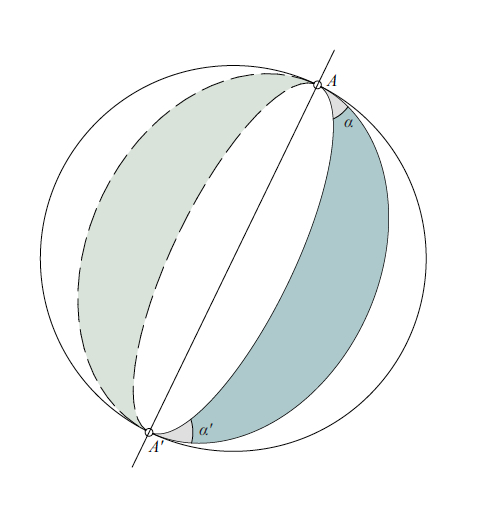
\includegraphics[width=0.3\textwidth]{kugel/Zweieck.jpg}
    \captionof{figure}{Bildung von Zweiecken durch Grosskreise}
\end{center}

Dabei ist der Flächeninhalt der ganzen Kugel:

\begin{align*}
A_{ Kugel } &= 4 \pi r^{2}
\end{align*}


Um den Flächeninhalt des betrachteten Zweieckes zu bekommen, 
müssen wir das ganze noch mit dem Kugelsegment mit dem Winkel $\alpha$ multiplizieren.

\begin{align*}
A_{ Zweieck } &= 4 \pi r^{2} \cdot \frac{ \alpha }{ 2 \pi }
\end{align*}


\subsection{Nicht Eulersche’ Dreiecke}

BLABLA

\subsection{Eulersche’ Dreiecke}

Legt man drei Grosskreise auf eine Kugeloberfläche, bilden sich dabei acht Dreiecke. 
Ein solches Dreieck heisst Eulersches’Dreieck\footnote{%
Leonard Euler (1707-1783), berühmter Schweizer Mathematiker und Physiker. 
Nicht Eulersche’Dreiecke erhält man, indem man das Äussere des Dreieckes ABC betrachtet.} 
Diese Dreiecke werden weder durch die Verlängerung ihrer Seiten durchschnitten, 
noch haben sie Dreiecksseiten welche grösser als $180^{\circ}$ sind.

\begin{center}
        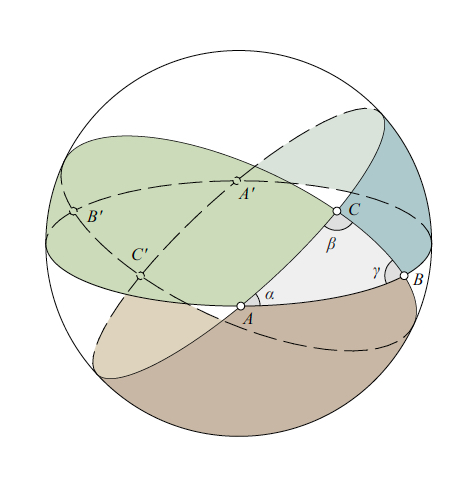
\includegraphics[width=0.4\textwidth]{kugel/Zweiecke.jpg}
    \captionof{figure}{Drei Grosskreise bilden ein sphärisches Dreieck}
\end{center}

In den nachstehenden Erklärungen und Herleitungen, sprechen wir ausschliesslich von Eulerschen’Dreiecken, da die umgeformten Winkelsätze der ebenen Trigonometrie nur auf diese Art von Kugeldreiecken angewendet werden kann.

$A_{ \overline{ ABC }}$ ist die Fläche des Dreieckes auf der Kugeloberfläche
In der ebenen Trigonometrie liegt die Winkelsumme eines Dreiecks bei
$180^{\circ}$.

Anders aber in der sphärischen Trigonometrie. Obschon sie einige Gemeinsamkeiten zur ebenen Trigonometrie aufweist, kann man nicht alles übernehmen.
So auch nicht wie Winkelsumme in einem sphärischen Dreieck.
Diese liegt bei:

\[
\begin{aligned}
\pi
&-
3\pi
&
&\text{\bigg \vert}
&
180^{\circ}
&-
540^{\circ}
\end{aligned}
\]

daraus lässt sich ableiten, das ein einzelner Winkel nicht grösser als $\pi$ oder $180^{\circ}$ sein darf. Ansonsten ist es kein Eulersches’Dreieck und wir dürfen die sphärische Trigonometrie nicht anwenden.\\
Wichtig anzumerken ist, dass die Seiten immer in Radiant beschrieben werden und nicht im Längenmass Meter wie wir es uns gewohnt sind. 
Bei den Dreiecksseiten handelt es sich um Kreisbögen und keine Strecken.

\section{Dreiecksfläche}

\begin{align*}
\text{Zweieck A}
&=
\overline{ABC} + \overline{A'BC} = 2 \alpha r^{ 2 } = A_{ \alpha }\\
\text{Zweieck B}
&=
\overline{ABC} + \overline{AB'C} = 2 \beta r^{ 2 } = A_{ \beta }\\
\text{Zweieck C}
&=
\overline{ABC} + \overline{ABC'} = 2 \gamma r^{ 2 } = A_{ \gamma }
\end{align*}

\begin{align*}
A_{ \alpha } + A_{ \beta } + A_{ \gamma } &= \frac{ 4\pi r^{ 2 } }{ 2 } + 2A_{ \overline{ ABC }} \\
2\alpha r^{ 2 } + 2\beta r^{ 2 } + 2\gamma r^{ 2 } &= \frac{ 4\pi r^{ 2 } }{ 2 } + 2A_{ \overline{ ABC }} \parallel:2\\
\alpha r^{ 2 } + \beta r^{ 2 } + \gamma r^{ 2 } &= \pi r^{ 2 } + A_{ \overline{ ABC }} \parallel-\pi r^{ 2 }\\
r^{ 2 }\left(\alpha + \beta + \gamma - \pi\right) &= A_{ \overline{ ABC }}
\end{align*}




\section{Sphärischer Exzess}
Die Winkelsumme sphärischer Dreiecke ist immer \textgreater \,  $\pi$.

\begin{align*}
\pi < \alpha + \beta + \gamma
\end{align*}

Der sphärische Exzess gibt dabei an, wie stark die Winkelsumme von $\pi$ abweicht.

\begin{align*}
\pi + \epsilon &= \alpha + \beta + \gamma \\
\epsilon &= \alpha + \beta + \gamma - \pi
\end{align*}

Würde der sphärische Exzess in der ebenen Trigonometrie angewendet, wäre dieser = 0. 
Bezieht man das auf die Erde und somit einer Kugel, kann man mit Hilfe eines beliebigen sphärischen Dreieckes und dessen Flächeninhalt auf den Radius der Kugel schliessen.

\subsection{Grenzfall - Satz von Legendre}

\begin{quote} \textit{Ein kleines sphärisches Dreieck kann näherungsweise 
wie ein ebenes Dreieck mit denselben Seiten berechnet 
werden, wenn alle Winkel des ebenen Dreiecks die um 
je ein Drittel des sphärischen Exzesses verminderten 
Winkel des sphärischen Dreiecks nimmt.} \end{quote}
\begin{flushright} - Adrien-Marie Legendre (1752-1833), Paris 1787
\end{flushright}x

Diese Aussage zeigt den Zusammenhang zwischen der 
Trigonometrie in der Ebene sowie in auf der Kugel
auf. Im speziellen bei sehr kleinen sphärischen 
Dreiecken ist die Winkelsumme nur unwesentlich 
grösser als $180^{\circ}$. Des Weiteren kann gesagt werden,
dass der sphärische Exzess gleichmässig auf alle
Winkel aufgeteilt wird.
Wichtig anzumerken ist, dass der Satz von Legendre 
für grosse, aber endliche Radien $r$ gilt.

%[SKIZZE GROSSER RADIUS/KLEINE KRÜMMUNG, KLEINER RADIUS/GROSSE KRÜMMUNG!!!!]
%


\section{Sphärisch Analoge Winkelfunktionen}

\subsection{Sphärischer Sinussatz}

Wir stellen die allgemeinen Sinussätze der Winkel $\alpha$ und $\gamma$ auf:


\[
\begin{aligned}
&{sin(\gamma)} = \frac{h}{a}
&
&\text{\bigg \vert}
&
&{sin(\alpha)} = \frac{h}{c}
&
\end{aligned}
\]

Daraus folgt:
\begin{align*}
h &= sin(\gamma)\cdot a \\
h &= sin(\alpha)\cdot c
\end{align*} 

Durch Gleichsetzung erhält man:
\begin{align*}
h &= h \\
sin(\gamma)\cdot a &= sin(\alpha)\cdot c
\end{align*} 

Durch umstellen erhalten wir den Sinussatz für a und c:
\begin{align*}
sin(\gamma)\cdot a &= sin(\alpha)\cdot c \\
\frac{sin(\gamma)}{c} &= \frac{sin(\alpha)}{a} 
\end{align*} 



\begin{align*}
\frac{sin(\alpha)}{sin(a)} = \frac{sin(\beta)}{sin(b)} = \frac{sin(\gamma)}{sin(c)}
\end{align*} 


\subsection{Winkelkosinussatz}

%[SKIZZE WINKELKOSINUS]

\[
\begin{aligned}
&\overline{C'A'} &= d\cdot {tan(b)}
&
&
&
&
&
&\overline{C'B'} &= d\cdot {tan(a)}
\end{aligned}
\]

\[
\begin{aligned}
&\overline{MA'} &= \frac{ d }{cos(b)}
&
&
&
&
&
&\overline{MB'} &= \frac{ d }{cos(a)}
\end{aligned}
\]

Der allgemeine Kosinussatz beschreibt sich wie folgt:

\begin{align*}
c^{ 2 } &= a^{ 2 } + b^{ 2 } - 2ab \cdot cos(\gamma)
\end{align*}

\begin{align*}
\triangle \overline{A'B'C' }
\overline{ A'B' }^{ 2 } &= \overline{ C'B' }^{ 2 } + \overline{ C'A' }^{ 2 } - 2 \cdot \overline{ C'B' } \cdot \overline{ C'A' } \cdot cos(\gamma)
\end{align*}



\begin{align*}
\overline{A'B'}^{ 2 } &= (d\cdot tan(a))^{ 2 } + (d\cdot tan(b))^{ 2 } - 2 \cdot (d\cdot tan(a) \cdot (d\cdot tan(b) \cdot cos(\gamma)\\
\overline{A'B'}^{ 2 } &= d^{ 2 } \cdot \left(\left(tan^{ 2 }(a) + tan^{ 2 }(b)\right) - 2\cdot tan(a) \cdot tan(b) \cdot cos(\gamma)\right)
\end{align*}

\begin{align*}
\triangle \overline{ MA'B' }
\overline{ A'B' }^{ 2 } &= \overline{ MB' }^{ 2 } + \overline{ MA' }^{ 2 } - 2\cdot \overline{ MB'} \cdot \overline{ MA' } \cdot cos(c)
\end{align*}


\begin{align*}
\overline{ A'B'}^{ 2 } &= \left(\frac{ d }{ cos(a) }  \right)^{ 2 } + \left(\frac{ d }{ cos(b)}  \right)^{ 2 } - 2 \cdot \frac{ d }{ cos(a)} \cdot \frac{ d }{ cos(b)} \cdot cos(c) \\
\overline{ A'B' }^{ 2 } &= d^{ 2 } \cdot \left(\left(\frac{ 1 }{ cos(a) }  \right)^{ 2 } + \left(\frac{ 1 }{ cos(b) }  \right)^{ 2 } - 2 \cdot \frac{ 1 }{ cos(a)} \cdot \frac{ 1 }{ cos(b)} \cdot cos(c)\right)\\
\overline{ A'B' }^{ 2 } &= d^{ 2 } \cdot \left(\left(tan^{ 2 }(a) + 1\right) + \left(tan^{ 2 }(b) + 1\right) - \left(2 \cdot \frac{cos(c)}{cos(a) \cdot cos(b)}\right)\right)
\end{align*}



\begin{align*}
\overline{ A'B'}^{ 2 } &= d^{ 2 } \cdot \left(\left(tan^{ 2 }(a) + tan^{ 2 }(b)\right) - 2 \cdot tan(a) \cdot tan(b) \cdot cos(\gamma)\right) \\
\overline{ A'B'}^{ 2 } &= d^{ 2 } \cdot \left(\left(tan^{ 2 }(a) + 1\right) + \left(tan^{ 2 }(b) + 1\right) - \left(2 \cdot \frac{cos(c)}{cos(a) \cdot cos(b)}\right)\right)
\end{align*}

Die anderen Gleichungen des Satzes, erfolgen aus Symmetriegründen.

\subsection{Seitenkosinussatz}
Durch zyklische Vertauschung des Winkelkosinus erhalten wir den Seitenkosinussatz:

\begin{align*}
{cos(a)} &= {cos(b)} \cdot {cos(c)} + {sin(b)} \cdot {sin(c)} \cdot {sin(\alpha)}\\
{cos(b)} &= {cos(a)} \cdot {cos(c)} + {sin(a)} \cdot {sin(c)} \cdot {sin(\beta)}\\
{cos(c)} &= {cos(a)} \cdot {cos(b)} + {sin(a)} \cdot {sin(b)} \cdot {sin(\gamma)}\\
\end{align*}

\section{Navigation auf See}
Das besondere an Seekarten ist die Inhaltliche Ausrichtung. Anders wie Landkarten muss sie Informationen enthalten welche für den Kapitän und seine Besatzung von grosser Bedeutung sind. Vor allem in Küstennähe ist das navigieren eines Schiffes besonders gefährlich. So enthalten Seekarten etwas über Wassertiefen, Bodenbeschaffenheiten, Gezeiten, Küstenlinien, Landzungen und Windrichtungen.
Der Hauptunterschied dabei ist, das auf der Landkarte feste Positionen definiert und aufgezeigt werden, das einzige was sich verändert ist der Reisende selbst. Bei der Seekarte ist das anders, es werden veränderliche Einwirkungen der Natur festgehalten.

Dieser kleine Unterschied zeigt die Notwendigkeit auf, die Position und den Kurs seines Schiffes auf See immer ermitteln zu können.


\section{Geographische Koordinaten}

Nachdem klar war, das die Erde eine Kugel ist, wurde diese in ein Gradnetz aufgeteilt. Dabei wurden die Angaben für eine exakte Ortsbestimmung klar definiert und die bis heute gültigen Koordinaten bestimmt.
Dabei muss man sich nochmals in Erinnerung rufen, dass sich die Erde in 24h einmal um ihre eigene Achse dreht. Nach $360 ^{\circ}$ 
und somit einer vollen Umdrehung, steht sie wieder in ihrer Ursprungsposition und ein neuer Tag beginnt.

Die Koordinaten setzen sich aus folgenden Komponenten zusammen:

\[
\begin{aligned}
&\text{Grad } (^{\circ})
&
&\text{\bigg \vert}
&
&\text{Bogenminuten } (`)
&
&\text{\bigg \vert}
&
&\text{Bogensekunden } (``)
\end{aligned}
\]

Die Erdoberfläche wurde in je 360 Breiten- und Längengrade eingeteilt. Die Breitengrade haben zueinander einen Abstand von 111.31 km, dies entspricht auch dem Abstand der Längengrade am Äquator mit Zunehmender Nähe zu den Polen, nimmt dieser Abstand ab.

\[
\begin{aligned}
&1^{\circ}
&
&\text{\bigg \vert}
&
&4 \text{ Minuten}
&
&\text{\bigg \vert}
&
&111.31\text{ km}
\end{aligned}
\]

Berechnet man nun die Erdumdrehung von 360°, erhält man genau den Erdumfang am Äquator: \begin{align*} 40’074 \text{ km.}\end{align*}

Dabei geben die Bogenminuten und -sekunden dem Standort die gewünschte Exaktheit. Mit den vollständigen Koordinaten lässt sich der Standort auf einer Landkarte exakt bestimmen und einzeichnen.

\subsection{Zeitzonen der Erde}
Wenn man nun die verschiedenen Zeitzonen der Erde betrachtet, macht die Verschiebung von jeweils einer Stunde durchaus Sinn, es lässt sich auf die Längengrade schliessen.
Zwischen den verschiedenen Zeitzonen liegen 15 Längengrade:

\begin{align*}
\text{15 Längengrade à 4 Minuten = 60 Minuten Zeitverschiebung = ca. 1665 km}
\end{align*}

Dabei ist die Zeitzone in welcher Mitte sich der Greenwich Meredian befindet die \textit{Greenwich Mean Time (GMT)} welche bis 1928 als Weltzeit galt. Im Jahr 1972 wurde diese umbenannt in die \textit{Coordinated Universal Time (UTC)} und wir von da an als Weltzeit $\pm$ 0.00 verwendet.


\section{Der Breitengrad}
Die Breitengrade bilden die bereits genannten Kleinkreise auf der Kugeloberfläche. Sie verlaufen in einem Abstand von genau 111 km parallel zum Äquator. Dabei stellt  dieser genau die Mitte zwischen Nord- und Südpol dar und teilt die Erdkugel in zwei gleiche Hälften. Somit wird von nördlicher und südlicher Breite gesprochen, je nach dem auf welcher Halbkugel man sich befindet.

%[SKIZZE DER GEOGRAFISCHEN BREITE ERDKUGEL]

\subsection{Geografische Breite $\phi$}
\begin{definition}
Die geografische Breite eines Standortes ist nichts anderes, als der Winkel am Erdmittelpunkt zwischen der Ebene des Äquators und der Geraden zum Standpunkt auf der Erdoberfläche.
\end{definition}

%[SKIZZE DER GEOGRAFISCHEN BREITE MIT WINKEL]

\subsection{Navigation mit den Breitengraden}
Da der Breitengrad bereits sehr früh ziemlich präzise bestimmt werden könnte, nutzten bereits die Seefahrer um Christoph Kolumbus den Breitengrad zur Navigation ihrer Flotten.
Den dieser lässt sich ziemlich einfach aus dem höchsten Sonnenstand oder einem Fixstern bestimmen. Dabei wird mit einem Jakobsstab\footnote{%
Der Jakobsstab ist ein früheres astronomisches Instrument zur Winkelmessung und wurde vor allem in der Seefahrt verwendet. Er ist in der Nautik der Vorläufer des Sextanten.} (später Sextant\footnote{%
Der Sextant ist ein nautisches Messinstrument zur Winkelmessung von Horizont und Fixstern (Gestirn)}) der Winkel zwischen dem Horizont und dem Fixstern gemessen. Der Winkel welchen man erhält, zieht man von 90° ab und erhält somit die geografische Breite. \\

%[SKIZZE ERMITTLUNG DES BREITENGRADES]

Wenn man sich auf der Nordhalbkugel befindet, ist der Polarstern ein sehr guter Fixstern. Befindet sich ein Schiff nun sehr nahe am Nordpol, steht dieser nahezu senkrecht am Himmelszelt bei $90^{\circ}$. Würde es aber nahe dem Äquator stehen, erscheint dieser am Horizont bei $0^{\circ}$.

\subsection{Korrekturbeiwert}

\section{Der Längengrad}
Die Längengrade bilden die bereits genannten Grosskreise auf der Kugeloberfläche.
Sie schneiden den Äquator im rechten Winkel, haben dort einen Abstand von 111 km zueinander und verbinden die Pole. Anders wie bei der geografischen Breite, ist in der Natur kein Längengrad gegeben welcher den Nullpunkt darstellt.

%[SKIZZE DER GEOGRAFISCHEN LÄNGE ERDKUGEL]

\subsection{Geografische Länge $\lambda$}
\begin{definition}
Die geografische Länge ist der Winkel an der Erdachse zum Nullmeridian.
\end{definition}

\subsection{Navigation mit den Längengraden}
Die geografische Länge lässt sich nicht so einfach bestimmen wie deren Breite. Für die Berechnung auf See benötigt man eine Referenzzeit eines Ortes mit bekannter Länge.
In der Zeit der Entdecker gab es noch keine mechanischen Uhren. Die Sonnenuhr war zudem ungeeignet, da diese nur die Uhrzeit am Standort mass und nicht die am Referenzort selbst. Die erste Pendeluhr wurde erst Mitte des 17. Jahrhunderts erfunden, was in der Schifffahrt aber auch nicht die Lösung brachte.\\
Pendeluhren auf einem Schiff sind ungeeignet, da das Pendel mit dem Wellengang aus dem Takt gebracht wird und somit die Uhr falsch geht.
Zu ungenau und gegen äussere Erschütterungen zu empfindlich waren später auch die federgetriebenen Uhren und die Unruh. Dazukamen die verschiedenen Klimazonen welche ein Schiff zu durchqueren hatten. Das Metall zog sich viel zu fest zusammen oder dehnte sich aus, was dazu führte das die Uhr unregelmässig lief.

Das sogenannte „Längenproblem“ stellte nicht nur bei der Navigation auf See ein Problem dar, es ergaben sich auch wirtschaftliche Konsequenzen. Die Schiffe mussten bis zur gewünschten geografischen Breite navigieren und segelten dann den Breitengrad entlang. Dabei waren die Schiffe oft Wochenlang unterwegs und segelten die „Breiten ab“ um an die gewünschte Position zu kommen. Dies führte zu erheblichen Zeitverlusten und viel längeren Reisezeiten.


\section{The Board of Longitude - Das Längenproblem}
Das Längenproblem beschäftigte alle grossen Seefahrernationen Europas. Wenn man bedenkt das sich Werte in einer  Höhe von halben britischen Staatshaushalten auf verloren gegangenen Schiffen befanden, erkennt man die Dringlichkeit für eine zuverlässige und genaue Navigation auf See.


\begin{itemize}
\item £ 20’000 - Abweichung von max. einem halben Grad
\item £ 15’000 - Abweichung von zwei Drittel Grad
\item £ 10’000 - Abweichung von max. $1 ^{\circ}$
\end{itemize}

\subsection{John Harrison}


\subsection{Tobias Mayer}



Uhren mit einer Abweichung von einer Minute Abweichung pro Tag (





\section{Nautische Dreieck}


$\Rightarrow$





\section{Die Vermessung der Welt}
Wir schreiben das Jahr 1818 und kehren in die Zeit des Mathematikers Carl Friedrich Gauss zurück. Neben dem liebevoll genannten „kleinen Gauss“ und anderen herausragenden Mathematischen Leistungen, beschäftigte er in den Folgejahren mit der Vermessung des Königreichs Hannovers und verfasste auf 61 Blättern das Kartenwerk \textit{Gauss’sche Landesaufnahme der 1815 durch Hannover erworbenen Gebiete}.






AUFGABE

Hubble Teleskop 
24. April 1990






\printbibliography[heading=subbibliography]
\end{refsection}




%\chapter{Geometrie auf der Kugeloberfläche\label{chapter:kugel}}
\lhead{Geometrie auf der Kugeloberfläche}
\begin{refsection}
\chapterauthor{Melina Staub und Fabian Schmid}

\section{Einleitung}

Schon seit jeher fasziniert den Menschen die Fahrt zur See. Nicht grundlos ist die Seefahrt eine der wichtigsten und ältesten Tätigkeiten der Menschheit. Der innerliche Drang neue Weltmeere und unbekannte Gebiete zu entdecken, die Fahrt zur See zu erleichtern und erträglicher zu machen, trieben die Menschen an, die Schiffe dieser Welt immer weiter zu entwickeln.

Die Idee der Kugelform der Erde ist älter als man zu denken vermag. Bereits der Schüler des antiken griechischen Philosophen Platon - Aristoteles schrieb in seiner Schrift \textit{Über den Himmel} aus dem 4. Jahrhundert v. Chr. etliche Gründe welche für die Gestallt der Erde als Kugel sprechen:

\begin{itemize}
      \item Sämtliche schweren Körper streben zum Mittelpunkt des Alls. Da sie dies von allen Seiten her gleichmäßig tun und die Erde im Mittelpunkt des Alls steht, muss sie eine kugelrunde Gestalt annehmen. 
\item Bei von der Küste wegfahrende Schiffen wird der Rumpf vor den Segeln der Sicht verborgen. 
\item In südlichen Ländern erscheinen südliche Sternbilder höher über dem Horizont.
\item Der Erdschatten bei einer Mondfinsternis ist stets rund.
\end{itemize}

Jedoch war um 1492 - der Zeit der Entdeckung Amerikas durch Christoph Kolumbus, die Idee der Erde in Kugelform noch sehr umstritten. Er erkannte anhand den Theorien und Erkenntnissen der alten Griechen, vor allem Aristoteles, das die Erde eine Kugel sein muss. \\
Doch mit seinem Vorschlag einen Seeweg über den Atlantik nach Indien zu finden und nicht wie üblich um Afrika zu segeln, stiess er beim beim portugiesischen König auf taube Ohren. Sein Plan Indien über eine Route nach Westen zu erreichen, widersprach dem gesunden Menschenverstand. Wäre die Erde wirklich eine Kugel und man befände sich auf der unteren Erdhalbkugel, würde man herunterfallen.\\
Doch auch der damals übliche Glaube an die Erde in Scheibenform brachte so einige Risiken mit sich. Was würde passieren, wenn die Flotte das Ende der Scheibe erreicht hatte? Würden sie über den Erdrand hinweggleiten und in den Abgrund stürzen?\\
Erst nach viel Überzeugungsarbeit durch Kolumbus, setzte er sich am Spanischen Hof durch und segelte über die Westliche Route über den Atlantik und entdeckte schlussendlich Amerika.

Der praktische und greifbare Beweis das die Erde eine Kugel ist, lieferte rund 30 Jahre später der Portugiese Fernando Magellan. Mit seiner Weltumsegelung und seiner Ankunft in den Philippinen, bewies er definitiv das die Erde eine Kugel ist.\\

Nun wollen wir uns die Frage stellen, wie die alten Seefahrer ohne GPS und jeglichen modernen Navigationssystemen auf hoher See wussten wo sie sich befinden und was haben die Sterne mit alldem zu tun? Reisen Sie mit uns zurück in eine Zeit mit Sextant, Kompass und Sternkarten. In die Zeit der Seefahrer und Entdecker.


\section{Geometrie auf der Ebene und der Kugel}

Euklid von Alexandria beschrieb die Grundbegriffe der ebenen Geometrie mittels Punkt, Geraden, Ebene, Winkel und Dreieck. Diese Dreiecke lassen sich mithilfe der ebenen Trigonometrie beschreiben. Dabei gelten die uns bekannten trigonometrischen Winkelfunktionen:\\

\text{Sinussatz:}
\begin{align*}
\frac{ a }{ sin(\alpha) } &= \frac{ b }{sin(\beta)} = \frac{ c }{ sin(\gamma) } = \frac{abc}{2A} = 2r\\
\end{align*}

\text{Cosinussatz:}
\begin{align*}
c^{ 2 } &= a^{ 2 } + b^{ 2 } - 2ab\cdot cos(\gamma)\\
b^{ 2 } &= a^{ 2 } + c^{ 2 } - 2ab\cdot cos(\beta)\\
a^{ 2 } &= b^{ 2 } + c^{ 2 } - 2ab\cdot cos(\alpha)
\end{align*}

Um Dreiecke auf der Kugeloberfläche zu berechnen, benötigt man die sphärische Trigonometrie. Die oben beschriebenen Sätze lassen sich auf der Kugel nicht anwenden, sie werden aber als Grundlage zur Herleitung der Sätze für das Kugeldreieck benötigt.

Die nachfolgenden Seiten thematisieren die Geometrie auf der Kugeloberfläche und wie sie in der Navigation eingesetzt werden kann.


\section{Gross- und Kleinkreise}

Eine Kugeloberfläche lässt sich in zwei verschiedene Kreisarten einteilen -  Gross- und Kleinkreise. 
Wir betrachten als erstes die Grosskreise:

\begin{definition}
Ein Großkreis ist ein größtmöglicher Kreis auf einer Kugeloberfläche. Sein Mittelpunkt fällt immer mit dem Mittelpunkt der Kugel zusammen und ein Schnitt auf dem Großkreis teilt die Kugel in jedem Fall in zwei („gleich große“) Hälften.
\end{definition}

Es gibt unendlich viele Möglichkeiten, eine Kugel in zwei gleich grosse Stücke zu zerschneiden, 
daher gibt es auch unendlich viele Grosskreise. Wenn wir die Grosskreise auf einer Kugel mit diesen auf der Erde beschreiben, sprechen wir von den Längengraden aber auch der Äquator beschreibt einen Grosskreis.
Ein Elementarer Bestandteil bilden die Grosskreise in der sphärischen Trigonometrie. Mithilfe der Schnittpunkte verschiedener Grosskreise, lässt sich ein Sphärisches Dreieck bilden auf welchem sich die sphärische Trigonometrie anwenden lässt.

[GRAFIK GROSSKREISE]

\begin{definition}
Unter Kleinkreis versteht man jene Kreise auf einer Kugeloberfläche, deren Ebenen nicht den Kugelmittelpunkt enthalten.
\end{definition}

Die Kleinkreise eignen sich im Gegensatz zu den Grosskreisen \textit{nicht} für die sphärische Trigonometrie. 
Sie werden lediglich zur Bestimmung der Messgrössen, Winkelabstände oder des Höhenwinkels eines Gestirns verwendet. 

Wenn wir die Kleinkreise auf die Erdoberfläche projizieren betrachten wir die Breitengrade.

[GRAFIK KLEINKREISE]


\section{Sphärische Dreiecke / Kugeldreieck}

\begin{center}
        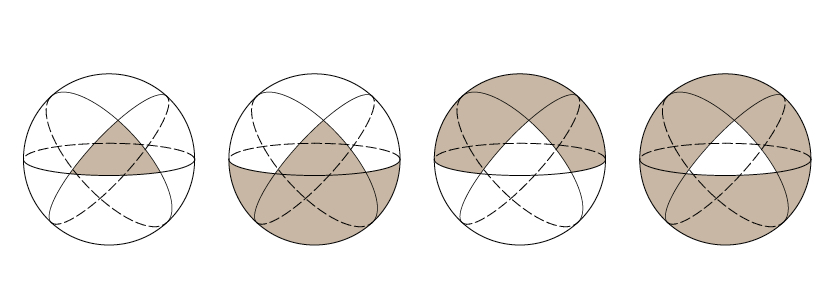
\includegraphics[width=0.9\textwidth]{kugel/Dreieckarten.jpg}
    \captionof{figure}{Dreieckarten auf einer Kugeloberfläche}
\end{center}

Der Begriff Sphärisches Dreieck oder Kugeldreieck ist ein sehr weitläufiger Begriff. 
Dabei können wir den Begriff in drei für uns wesentliche Dreiecke unterteilen:

\begin{itemize}
\item Kugelzweieck
\item Nicht Eulersche’Dreiecke
\item Eulersche’Dreiecke
\end{itemize}

\subsection{Kugelzweieck}

Zwei Grosskreise auf der Kugeloberfläche, zerlegen diese in vier gleiche Kugelzweiecke. 
Jedes dieser Dreieckseiten hat die Länge
$180^{\circ}$ oder $\pi$
Der Flächeninhalt wird dabei nur durch den Winkel $\alpha$ zwischen den beiden Grosskreisen bestimmt.

\begin{center}
        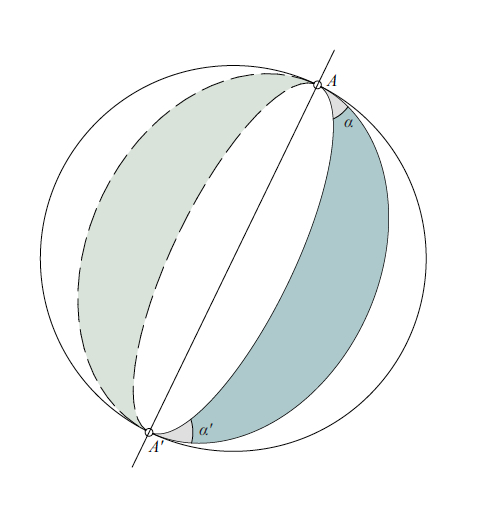
\includegraphics[width=0.3\textwidth]{kugel/Zweieck.jpg}
    \captionof{figure}{Bildung von Zweiecken durch Grosskreise}
\end{center}

Dabei ist der Flächeninhalt der ganzen Kugel:

\begin{align*}
A_{ Kugel } &= 4 \pi r^{2}
\end{align*}


Um den Flächeninhalt des betrachteten Zweieckes zu bekommen, 
müssen wir das ganze noch mit dem Kugelsegment mit dem Winkel $\alpha$ multiplizieren.

\begin{align*}
A_{ Zweieck } &= 4 \pi r^{2} \cdot \frac{ \alpha }{ 2 \pi }
\end{align*}


\subsection{Nicht Eulersche’ Dreiecke}

BLABLA

\subsection{Eulersche’ Dreiecke}

Legt man drei Grosskreise auf eine Kugeloberfläche, bilden sich dabei acht Dreiecke. 
Ein solches Dreieck heisst Eulersches’Dreieck\footnote{%
Leonard Euler (1707-1783), berühmter Schweizer Mathematiker und Physiker. 
Nicht Eulersche’Dreiecke erhält man, indem man das Äussere des Dreieckes ABC betrachtet.} 
Diese Dreiecke werden weder durch die Verlängerung ihrer Seiten durchschnitten, 
noch haben sie Dreiecksseiten welche grösser als $180^{\circ}$ sind.

\begin{center}
        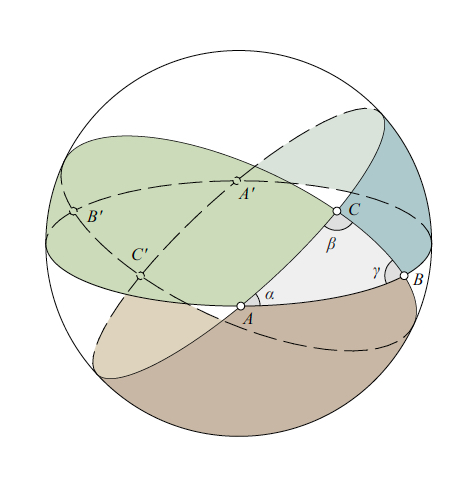
\includegraphics[width=0.4\textwidth]{kugel/Zweiecke.jpg}
    \captionof{figure}{Drei Grosskreise bilden ein sphärisches Dreieck}
\end{center}

In den nachstehenden Erklärungen und Herleitungen, sprechen wir ausschliesslich von Eulerschen’Dreiecken, da die umgeformten Winkelsätze der ebenen Trigonometrie nur auf diese Art von Kugeldreiecken angewendet werden kann.

$A_{ \overline{ ABC }}$ ist die Fläche des Dreieckes auf der Kugeloberfläche
In der ebenen Trigonometrie liegt die Winkelsumme eines Dreiecks bei
$180^{\circ}$.

Anders aber in der sphärischen Trigonometrie. Obschon sie einige Gemeinsamkeiten zur ebenen Trigonometrie aufweist, kann man nicht alles übernehmen.
So auch nicht wie Winkelsumme in einem sphärischen Dreieck.
Diese liegt bei:

\[
\begin{aligned}
\pi
&-
3\pi
&
&\text{\bigg \vert}
&
180^{\circ}
&-
540^{\circ}
\end{aligned}
\]

daraus lässt sich ableiten, das ein einzelner Winkel nicht grösser als $\pi$ oder $180^{\circ}$ sein darf. Ansonsten ist es kein Eulersches’Dreieck und wir dürfen die sphärische Trigonometrie nicht anwenden.\\
Wichtig anzumerken ist, dass die Seiten immer in Radiant beschrieben werden und nicht im Längenmass Meter wie wir es uns gewohnt sind. 
Bei den Dreiecksseiten handelt es sich um Kreisbögen und keine Strecken.

\section{Dreiecksfläche}

\begin{align*}
\text{Zweieck A}
&=
\overline{ABC} + \overline{A'BC} = 2 \alpha r^{ 2 } = A_{ \alpha }\\
\text{Zweieck B}
&=
\overline{ABC} + \overline{AB'C} = 2 \beta r^{ 2 } = A_{ \beta }\\
\text{Zweieck C}
&=
\overline{ABC} + \overline{ABC'} = 2 \gamma r^{ 2 } = A_{ \gamma }
\end{align*}

\begin{align*}
A_{ \alpha } + A_{ \beta } + A_{ \gamma } &= \frac{ 4\pi r^{ 2 } }{ 2 } + 2A_{ \overline{ ABC }} \\
2\alpha r^{ 2 } + 2\beta r^{ 2 } + 2\gamma r^{ 2 } &= \frac{ 4\pi r^{ 2 } }{ 2 } + 2A_{ \overline{ ABC }} \parallel:2\\
\alpha r^{ 2 } + \beta r^{ 2 } + \gamma r^{ 2 } &= \pi r^{ 2 } + A_{ \overline{ ABC }} \parallel-\pi r^{ 2 }\\
r^{ 2 }\left(\alpha + \beta + \gamma - \pi\right) &= A_{ \overline{ ABC }}
\end{align*}




\section{Sphärischer Exzess}
Die Winkelsumme sphärischer Dreiecke ist immer \textgreater \,  $\pi$.

\begin{align*}
\pi < \alpha + \beta + \gamma
\end{align*}

Der sphärische Exzess gibt dabei an, wie stark die Winkelsumme von $\pi$ abweicht.

\begin{align*}
\pi + \epsilon &= \alpha + \beta + \gamma \\
\epsilon &= \alpha + \beta + \gamma - \pi
\end{align*}

Würde der sphärische Exzess in der ebenen Trigonometrie angewendet, wäre dieser = 0. 
Bezieht man das auf die Erde und somit einer Kugel, kann man mit Hilfe eines beliebigen sphärischen Dreieckes und dessen Flächeninhalt auf den Radius der Kugel schliessen.

\subsection{Grenzfall - Satz von Legendre}

\begin{quote} \textit{Ein kleines sphärisches Dreieck kann näherungsweise 
wie ein ebenes Dreieck mit denselben Seiten berechnet 
werden, wenn alle Winkel des ebenen Dreiecks die um 
je ein Drittel des sphärischen Exzesses verminderten 
Winkel des sphärischen Dreiecks nimmt.} \end{quote}
\begin{flushright} - Adrien-Marie Legendre (1752-1833), Paris 1787
\end{flushright}x

Diese Aussage zeigt den Zusammenhang zwischen der 
Trigonometrie in der Ebene sowie in auf der Kugel
auf. Im speziellen bei sehr kleinen sphärischen 
Dreiecken ist die Winkelsumme nur unwesentlich 
grösser als $180^{\circ}$. Des Weiteren kann gesagt werden,
dass der sphärische Exzess gleichmässig auf alle
Winkel aufgeteilt wird.
Wichtig anzumerken ist, dass der Satz von Legendre 
für grosse, aber endliche Radien $r$ gilt.

%[SKIZZE GROSSER RADIUS/KLEINE KRÜMMUNG, KLEINER RADIUS/GROSSE KRÜMMUNG!!!!]
%


\section{Sphärisch Analoge Winkelfunktionen}

\subsection{Sphärischer Sinussatz}

Wir stellen die allgemeinen Sinussätze der Winkel $\alpha$ und $\gamma$ auf:


\[
\begin{aligned}
&{sin(\gamma)} = \frac{h}{a}
&
&\text{\bigg \vert}
&
&{sin(\alpha)} = \frac{h}{c}
&
\end{aligned}
\]

Daraus folgt:
\begin{align*}
h &= sin(\gamma)\cdot a \\
h &= sin(\alpha)\cdot c
\end{align*} 

Durch Gleichsetzung erhält man:
\begin{align*}
h &= h \\
sin(\gamma)\cdot a &= sin(\alpha)\cdot c
\end{align*} 

Durch umstellen erhalten wir den Sinussatz für a und c:
\begin{align*}
sin(\gamma)\cdot a &= sin(\alpha)\cdot c \\
\frac{sin(\gamma)}{c} &= \frac{sin(\alpha)}{a} 
\end{align*} 



\begin{align*}
\frac{sin(\alpha)}{sin(a)} = \frac{sin(\beta)}{sin(b)} = \frac{sin(\gamma)}{sin(c)}
\end{align*} 


\subsection{Winkelkosinussatz}

%[SKIZZE WINKELKOSINUS]

\[
\begin{aligned}
&\overline{C'A'} &= d\cdot {tan(b)}
&
&
&
&
&
&\overline{C'B'} &= d\cdot {tan(a)}
\end{aligned}
\]

\[
\begin{aligned}
&\overline{MA'} &= \frac{ d }{cos(b)}
&
&
&
&
&
&\overline{MB'} &= \frac{ d }{cos(a)}
\end{aligned}
\]

Der allgemeine Kosinussatz beschreibt sich wie folgt:

\begin{align*}
c^{ 2 } &= a^{ 2 } + b^{ 2 } - 2ab \cdot cos(\gamma)
\end{align*}

\begin{align*}
\triangle \overline{A'B'C' }
\overline{ A'B' }^{ 2 } &= \overline{ C'B' }^{ 2 } + \overline{ C'A' }^{ 2 } - 2 \cdot \overline{ C'B' } \cdot \overline{ C'A' } \cdot cos(\gamma)
\end{align*}



\begin{align*}
\overline{A'B'}^{ 2 } &= (d\cdot tan(a))^{ 2 } + (d\cdot tan(b))^{ 2 } - 2 \cdot (d\cdot tan(a) \cdot (d\cdot tan(b) \cdot cos(\gamma)\\
\overline{A'B'}^{ 2 } &= d^{ 2 } \cdot \left(\left(tan^{ 2 }(a) + tan^{ 2 }(b)\right) - 2\cdot tan(a) \cdot tan(b) \cdot cos(\gamma)\right)
\end{align*}

\begin{align*}
\triangle \overline{ MA'B' }
\overline{ A'B' }^{ 2 } &= \overline{ MB' }^{ 2 } + \overline{ MA' }^{ 2 } - 2\cdot \overline{ MB'} \cdot \overline{ MA' } \cdot cos(c)
\end{align*}


\begin{align*}
\overline{ A'B'}^{ 2 } &= \left(\frac{ d }{ cos(a) }  \right)^{ 2 } + \left(\frac{ d }{ cos(b)}  \right)^{ 2 } - 2 \cdot \frac{ d }{ cos(a)} \cdot \frac{ d }{ cos(b)} \cdot cos(c) \\
\overline{ A'B' }^{ 2 } &= d^{ 2 } \cdot \left(\left(\frac{ 1 }{ cos(a) }  \right)^{ 2 } + \left(\frac{ 1 }{ cos(b) }  \right)^{ 2 } - 2 \cdot \frac{ 1 }{ cos(a)} \cdot \frac{ 1 }{ cos(b)} \cdot cos(c)\right)\\
\overline{ A'B' }^{ 2 } &= d^{ 2 } \cdot \left(\left(tan^{ 2 }(a) + 1\right) + \left(tan^{ 2 }(b) + 1\right) - \left(2 \cdot \frac{cos(c)}{cos(a) \cdot cos(b)}\right)\right)
\end{align*}



\begin{align*}
\overline{ A'B'}^{ 2 } &= d^{ 2 } \cdot \left(\left(tan^{ 2 }(a) + tan^{ 2 }(b)\right) - 2 \cdot tan(a) \cdot tan(b) \cdot cos(\gamma)\right) \\
\overline{ A'B'}^{ 2 } &= d^{ 2 } \cdot \left(\left(tan^{ 2 }(a) + 1\right) + \left(tan^{ 2 }(b) + 1\right) - \left(2 \cdot \frac{cos(c)}{cos(a) \cdot cos(b)}\right)\right)
\end{align*}

Die anderen Gleichungen des Satzes, erfolgen aus Symmetriegründen.

\subsection{Seitenkosinussatz}
Durch zyklische Vertauschung des Winkelkosinus erhalten wir den Seitenkosinussatz:

\begin{align*}
{cos(a)} &= {cos(b)} \cdot {cos(c)} + {sin(b)} \cdot {sin(c)} \cdot {sin(\alpha)}\\
{cos(b)} &= {cos(a)} \cdot {cos(c)} + {sin(a)} \cdot {sin(c)} \cdot {sin(\beta)}\\
{cos(c)} &= {cos(a)} \cdot {cos(b)} + {sin(a)} \cdot {sin(b)} \cdot {sin(\gamma)}\\
\end{align*}

\section{Navigation auf See}
Das besondere an Seekarten ist die Inhaltliche Ausrichtung. Anders wie Landkarten muss sie Informationen enthalten welche für den Kapitän und seine Besatzung von grosser Bedeutung sind. Vor allem in Küstennähe ist das navigieren eines Schiffes besonders gefährlich. So enthalten Seekarten etwas über Wassertiefen, Bodenbeschaffenheiten, Gezeiten, Küstenlinien, Landzungen und Windrichtungen.
Der Hauptunterschied dabei ist, das auf der Landkarte feste Positionen definiert und aufgezeigt werden, das einzige was sich verändert ist der Reisende selbst. Bei der Seekarte ist das anders, es werden veränderliche Einwirkungen der Natur festgehalten.

Dieser kleine Unterschied zeigt die Notwendigkeit auf, die Position und den Kurs seines Schiffes auf See immer ermitteln zu können.


\section{Geographische Koordinaten}

Nachdem klar war, das die Erde eine Kugel ist, wurde diese in ein Gradnetz aufgeteilt. Dabei wurden die Angaben für eine exakte Ortsbestimmung klar definiert und die bis heute gültigen Koordinaten bestimmt.
Dabei muss man sich nochmals in Erinnerung rufen, dass sich die Erde in 24h einmal um ihre eigene Achse dreht. Nach $360 ^{\circ}$ 
und somit einer vollen Umdrehung, steht sie wieder in ihrer Ursprungsposition und ein neuer Tag beginnt.

Die Koordinaten setzen sich aus folgenden Komponenten zusammen:

\[
\begin{aligned}
&\text{Grad } (^{\circ})
&
&\text{\bigg \vert}
&
&\text{Bogenminuten } (`)
&
&\text{\bigg \vert}
&
&\text{Bogensekunden } (``)
\end{aligned}
\]

Die Erdoberfläche wurde in je 360 Breiten- und Längengrade eingeteilt. Die Breitengrade haben zueinander einen Abstand von 111.31 km, dies entspricht auch dem Abstand der Längengrade am Äquator mit Zunehmender Nähe zu den Polen, nimmt dieser Abstand ab.

\[
\begin{aligned}
&1^{\circ}
&
&\text{\bigg \vert}
&
&4 \text{ Minuten}
&
&\text{\bigg \vert}
&
&111.31\text{ km}
\end{aligned}
\]

Berechnet man nun die Erdumdrehung von 360°, erhält man genau den Erdumfang am Äquator: \begin{align*} 40’074 \text{ km.}\end{align*}

Dabei geben die Bogenminuten und -sekunden dem Standort die gewünschte Exaktheit. Mit den vollständigen Koordinaten lässt sich der Standort auf einer Landkarte exakt bestimmen und einzeichnen.

\subsection{Zeitzonen der Erde}
Wenn man nun die verschiedenen Zeitzonen der Erde betrachtet, macht die Verschiebung von jeweils einer Stunde durchaus Sinn, es lässt sich auf die Längengrade schliessen.
Zwischen den verschiedenen Zeitzonen liegen 15 Längengrade:

\begin{align*}
\text{15 Längengrade à 4 Minuten = 60 Minuten Zeitverschiebung = ca. 1665 km}
\end{align*}

Dabei ist die Zeitzone in welcher Mitte sich der Greenwich Meredian befindet die \textit{Greenwich Mean Time (GMT)} welche bis 1928 als Weltzeit galt. Im Jahr 1972 wurde diese umbenannt in die \textit{Coordinated Universal Time (UTC)} und wir von da an als Weltzeit $\pm$ 0.00 verwendet.


\section{Der Breitengrad}
Die Breitengrade bilden die bereits genannten Kleinkreise auf der Kugeloberfläche. Sie verlaufen in einem Abstand von genau 111 km parallel zum Äquator. Dabei stellt  dieser genau die Mitte zwischen Nord- und Südpol dar und teilt die Erdkugel in zwei gleiche Hälften. Somit wird von nördlicher und südlicher Breite gesprochen, je nach dem auf welcher Halbkugel man sich befindet.

%[SKIZZE DER GEOGRAFISCHEN BREITE ERDKUGEL]

\subsection{Geografische Breite $\phi$}
\begin{definition}
Die geografische Breite eines Standortes ist nichts anderes, als der Winkel am Erdmittelpunkt zwischen der Ebene des Äquators und der Geraden zum Standpunkt auf der Erdoberfläche.
\end{definition}

%[SKIZZE DER GEOGRAFISCHEN BREITE MIT WINKEL]

\subsection{Navigation mit den Breitengraden}
Da der Breitengrad bereits sehr früh ziemlich präzise bestimmt werden könnte, nutzten bereits die Seefahrer um Christoph Kolumbus den Breitengrad zur Navigation ihrer Flotten.
Den dieser lässt sich ziemlich einfach aus dem höchsten Sonnenstand oder einem Fixstern bestimmen. Dabei wird mit einem Jakobsstab\footnote{%
Der Jakobsstab ist ein früheres astronomisches Instrument zur Winkelmessung und wurde vor allem in der Seefahrt verwendet. Er ist in der Nautik der Vorläufer des Sextanten.} (später Sextant\footnote{%
Der Sextant ist ein nautisches Messinstrument zur Winkelmessung von Horizont und Fixstern (Gestirn)}) der Winkel zwischen dem Horizont und dem Fixstern gemessen. Der Winkel welchen man erhält, zieht man von 90° ab und erhält somit die geografische Breite. \\

%[SKIZZE ERMITTLUNG DES BREITENGRADES]

Wenn man sich auf der Nordhalbkugel befindet, ist der Polarstern ein sehr guter Fixstern. Befindet sich ein Schiff nun sehr nahe am Nordpol, steht dieser nahezu senkrecht am Himmelszelt bei $90^{\circ}$. Würde es aber nahe dem Äquator stehen, erscheint dieser am Horizont bei $0^{\circ}$.

\subsection{Korrekturbeiwert}

\section{Der Längengrad}
Die Längengrade bilden die bereits genannten Grosskreise auf der Kugeloberfläche.
Sie schneiden den Äquator im rechten Winkel, haben dort einen Abstand von 111 km zueinander und verbinden die Pole. Anders wie bei der geografischen Breite, ist in der Natur kein Längengrad gegeben welcher den Nullpunkt darstellt.

%[SKIZZE DER GEOGRAFISCHEN LÄNGE ERDKUGEL]

\subsection{Geografische Länge $\lambda$}
\begin{definition}
Die geografische Länge ist der Winkel an der Erdachse zum Nullmeridian.
\end{definition}

\subsection{Navigation mit den Längengraden}
Die geografische Länge lässt sich nicht so einfach bestimmen wie deren Breite. Für die Berechnung auf See benötigt man eine Referenzzeit eines Ortes mit bekannter Länge.
In der Zeit der Entdecker gab es noch keine mechanischen Uhren. Die Sonnenuhr war zudem ungeeignet, da diese nur die Uhrzeit am Standort mass und nicht die am Referenzort selbst. Die erste Pendeluhr wurde erst Mitte des 17. Jahrhunderts erfunden, was in der Schifffahrt aber auch nicht die Lösung brachte.\\
Pendeluhren auf einem Schiff sind ungeeignet, da das Pendel mit dem Wellengang aus dem Takt gebracht wird und somit die Uhr falsch geht.
Zu ungenau und gegen äussere Erschütterungen zu empfindlich waren später auch die federgetriebenen Uhren und die Unruh. Dazukamen die verschiedenen Klimazonen welche ein Schiff zu durchqueren hatten. Das Metall zog sich viel zu fest zusammen oder dehnte sich aus, was dazu führte das die Uhr unregelmässig lief.

Das sogenannte „Längenproblem“ stellte nicht nur bei der Navigation auf See ein Problem dar, es ergaben sich auch wirtschaftliche Konsequenzen. Die Schiffe mussten bis zur gewünschten geografischen Breite navigieren und segelten dann den Breitengrad entlang. Dabei waren die Schiffe oft Wochenlang unterwegs und segelten die „Breiten ab“ um an die gewünschte Position zu kommen. Dies führte zu erheblichen Zeitverlusten und viel längeren Reisezeiten.


\section{The Board of Longitude - Das Längenproblem}
Das Längenproblem beschäftigte alle grossen Seefahrernationen Europas. Wenn man bedenkt das sich Werte in einer  Höhe von halben britischen Staatshaushalten auf verloren gegangenen Schiffen befanden, erkennt man die Dringlichkeit für eine zuverlässige und genaue Navigation auf See.


\begin{itemize}
\item £ 20’000 - Abweichung von max. einem halben Grad
\item £ 15’000 - Abweichung von zwei Drittel Grad
\item £ 10’000 - Abweichung von max. $1 ^{\circ}$
\end{itemize}

\subsection{John Harrison}


\subsection{Tobias Mayer}



Uhren mit einer Abweichung von einer Minute Abweichung pro Tag (





\section{Nautische Dreieck}


$\Rightarrow$





\section{Die Vermessung der Welt}
Wir schreiben das Jahr 1818 und kehren in die Zeit des Mathematikers Carl Friedrich Gauss zurück. Neben dem liebevoll genannten „kleinen Gauss“ und anderen herausragenden Mathematischen Leistungen, beschäftigte er in den Folgejahren mit der Vermessung des Königreichs Hannovers und verfasste auf 61 Blättern das Kartenwerk \textit{Gauss’sche Landesaufnahme der 1815 durch Hannover erworbenen Gebiete}.






AUFGABE

Hubble Teleskop 
24. April 1990






\printbibliography[heading=subbibliography]
\end{refsection}




%\chapter{Geometrie auf der Kugeloberfläche\label{chapter:kugel}}
\lhead{Geometrie auf der Kugeloberfläche}
\begin{refsection}
\chapterauthor{Melina Staub und Fabian Schmid}

\section{Einleitung}

Schon seit jeher fasziniert den Menschen die Fahrt zur See. Nicht grundlos ist die Seefahrt eine der wichtigsten und ältesten Tätigkeiten der Menschheit. Der innerliche Drang neue Weltmeere und unbekannte Gebiete zu entdecken, die Fahrt zur See zu erleichtern und erträglicher zu machen, trieben die Menschen an, die Schiffe dieser Welt immer weiter zu entwickeln.

Die Idee der Kugelform der Erde ist älter als man zu denken vermag. Bereits der Schüler des antiken griechischen Philosophen Platon - Aristoteles schrieb in seiner Schrift \textit{Über den Himmel} aus dem 4. Jahrhundert v. Chr. etliche Gründe welche für die Gestallt der Erde als Kugel sprechen:

\begin{itemize}
      \item Sämtliche schweren Körper streben zum Mittelpunkt des Alls. Da sie dies von allen Seiten her gleichmäßig tun und die Erde im Mittelpunkt des Alls steht, muss sie eine kugelrunde Gestalt annehmen. 
\item Bei von der Küste wegfahrende Schiffen wird der Rumpf vor den Segeln der Sicht verborgen. 
\item In südlichen Ländern erscheinen südliche Sternbilder höher über dem Horizont.
\item Der Erdschatten bei einer Mondfinsternis ist stets rund.
\end{itemize}

Jedoch war um 1492 - der Zeit der Entdeckung Amerikas durch Christoph Kolumbus, die Idee der Erde in Kugelform noch sehr umstritten. Er erkannte anhand den Theorien und Erkenntnissen der alten Griechen, vor allem Aristoteles, das die Erde eine Kugel sein muss. \\
Doch mit seinem Vorschlag einen Seeweg über den Atlantik nach Indien zu finden und nicht wie üblich um Afrika zu segeln, stiess er beim beim portugiesischen König auf taube Ohren. Sein Plan Indien über eine Route nach Westen zu erreichen, widersprach dem gesunden Menschenverstand. Wäre die Erde wirklich eine Kugel und man befände sich auf der unteren Erdhalbkugel, würde man herunterfallen.\\
Doch auch der damals übliche Glaube an die Erde in Scheibenform brachte so einige Risiken mit sich. Was würde passieren, wenn die Flotte das Ende der Scheibe erreicht hatte? Würden sie über den Erdrand hinweggleiten und in den Abgrund stürzen?\\
Erst nach viel Überzeugungsarbeit durch Kolumbus, setzte er sich am Spanischen Hof durch und segelte über die Westliche Route über den Atlantik und entdeckte schlussendlich Amerika.

Der praktische und greifbare Beweis das die Erde eine Kugel ist, lieferte rund 30 Jahre später der Portugiese Fernando Magellan. Mit seiner Weltumsegelung und seiner Ankunft in den Philippinen, bewies er definitiv das die Erde eine Kugel ist.\\

Nun wollen wir uns die Frage stellen, wie die alten Seefahrer ohne GPS und jeglichen modernen Navigationssystemen auf hoher See wussten wo sie sich befinden und was haben die Sterne mit alldem zu tun? Reisen Sie mit uns zurück in eine Zeit mit Sextant, Kompass und Sternkarten. In die Zeit der Seefahrer und Entdecker.


\section{Geometrie auf der Ebene und der Kugel}

Euklid von Alexandria beschrieb die Grundbegriffe der ebenen Geometrie mittels Punkt, Geraden, Ebene, Winkel und Dreieck. Diese Dreiecke lassen sich mithilfe der ebenen Trigonometrie beschreiben. Dabei gelten die uns bekannten trigonometrischen Winkelfunktionen:\\

\text{Sinussatz:}
\begin{align*}
\frac{ a }{ sin(\alpha) } &= \frac{ b }{sin(\beta)} = \frac{ c }{ sin(\gamma) } = \frac{abc}{2A} = 2r\\
\end{align*}

\text{Cosinussatz:}
\begin{align*}
c^{ 2 } &= a^{ 2 } + b^{ 2 } - 2ab\cdot cos(\gamma)\\
b^{ 2 } &= a^{ 2 } + c^{ 2 } - 2ab\cdot cos(\beta)\\
a^{ 2 } &= b^{ 2 } + c^{ 2 } - 2ab\cdot cos(\alpha)
\end{align*}

Um Dreiecke auf der Kugeloberfläche zu berechnen, benötigt man die sphärische Trigonometrie. Die oben beschriebenen Sätze lassen sich auf der Kugel nicht anwenden, sie werden aber als Grundlage zur Herleitung der Sätze für das Kugeldreieck benötigt.

Die nachfolgenden Seiten thematisieren die Geometrie auf der Kugeloberfläche und wie sie in der Navigation eingesetzt werden kann.


\section{Gross- und Kleinkreise}

Eine Kugeloberfläche lässt sich in zwei verschiedene Kreisarten einteilen -  Gross- und Kleinkreise. 
Wir betrachten als erstes die Grosskreise:

\begin{definition}
Ein Großkreis ist ein größtmöglicher Kreis auf einer Kugeloberfläche. Sein Mittelpunkt fällt immer mit dem Mittelpunkt der Kugel zusammen und ein Schnitt auf dem Großkreis teilt die Kugel in jedem Fall in zwei („gleich große“) Hälften.
\end{definition}

Es gibt unendlich viele Möglichkeiten, eine Kugel in zwei gleich grosse Stücke zu zerschneiden, 
daher gibt es auch unendlich viele Grosskreise. Wenn wir die Grosskreise auf einer Kugel mit diesen auf der Erde beschreiben, sprechen wir von den Längengraden aber auch der Äquator beschreibt einen Grosskreis.
Ein Elementarer Bestandteil bilden die Grosskreise in der sphärischen Trigonometrie. Mithilfe der Schnittpunkte verschiedener Grosskreise, lässt sich ein Sphärisches Dreieck bilden auf welchem sich die sphärische Trigonometrie anwenden lässt.

[GRAFIK GROSSKREISE]

\begin{definition}
Unter Kleinkreis versteht man jene Kreise auf einer Kugeloberfläche, deren Ebenen nicht den Kugelmittelpunkt enthalten.
\end{definition}

Die Kleinkreise eignen sich im Gegensatz zu den Grosskreisen \textit{nicht} für die sphärische Trigonometrie. 
Sie werden lediglich zur Bestimmung der Messgrössen, Winkelabstände oder des Höhenwinkels eines Gestirns verwendet. 

Wenn wir die Kleinkreise auf die Erdoberfläche projizieren betrachten wir die Breitengrade.

[GRAFIK KLEINKREISE]


\section{Sphärische Dreiecke / Kugeldreieck}

\begin{center}
        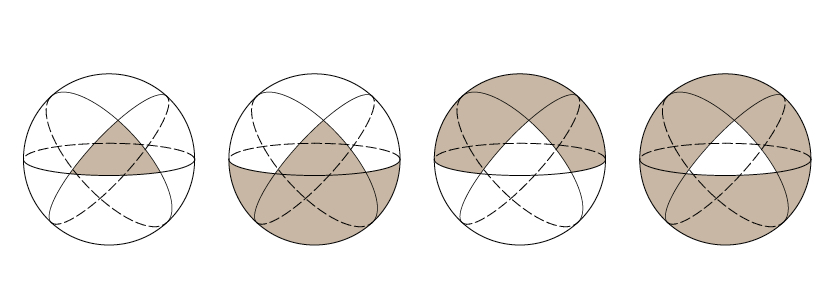
\includegraphics[width=0.9\textwidth]{kugel/Dreieckarten.jpg}
    \captionof{figure}{Dreieckarten auf einer Kugeloberfläche}
\end{center}

Der Begriff Sphärisches Dreieck oder Kugeldreieck ist ein sehr weitläufiger Begriff. 
Dabei können wir den Begriff in drei für uns wesentliche Dreiecke unterteilen:

\begin{itemize}
\item Kugelzweieck
\item Nicht Eulersche’Dreiecke
\item Eulersche’Dreiecke
\end{itemize}

\subsection{Kugelzweieck}

Zwei Grosskreise auf der Kugeloberfläche, zerlegen diese in vier gleiche Kugelzweiecke. 
Jedes dieser Dreieckseiten hat die Länge
$180^{\circ}$ oder $\pi$
Der Flächeninhalt wird dabei nur durch den Winkel $\alpha$ zwischen den beiden Grosskreisen bestimmt.

\begin{center}
        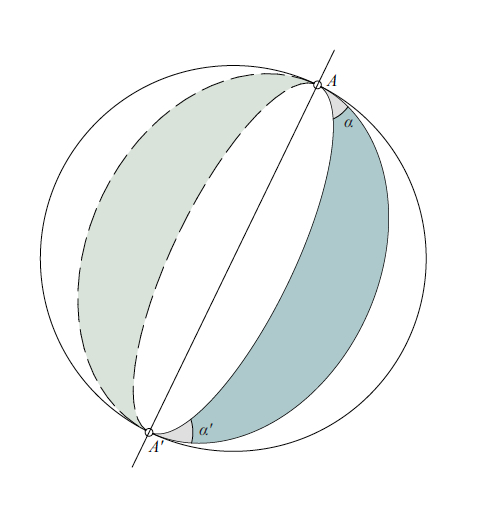
\includegraphics[width=0.3\textwidth]{kugel/Zweieck.jpg}
    \captionof{figure}{Bildung von Zweiecken durch Grosskreise}
\end{center}

Dabei ist der Flächeninhalt der ganzen Kugel:

\begin{align*}
A_{ Kugel } &= 4 \pi r^{2}
\end{align*}


Um den Flächeninhalt des betrachteten Zweieckes zu bekommen, 
müssen wir das ganze noch mit dem Kugelsegment mit dem Winkel $\alpha$ multiplizieren.

\begin{align*}
A_{ Zweieck } &= 4 \pi r^{2} \cdot \frac{ \alpha }{ 2 \pi }
\end{align*}


\subsection{Nicht Eulersche’ Dreiecke}

BLABLA

\subsection{Eulersche’ Dreiecke}

Legt man drei Grosskreise auf eine Kugeloberfläche, bilden sich dabei acht Dreiecke. 
Ein solches Dreieck heisst Eulersches’Dreieck\footnote{%
Leonard Euler (1707-1783), berühmter Schweizer Mathematiker und Physiker. 
Nicht Eulersche’Dreiecke erhält man, indem man das Äussere des Dreieckes ABC betrachtet.} 
Diese Dreiecke werden weder durch die Verlängerung ihrer Seiten durchschnitten, 
noch haben sie Dreiecksseiten welche grösser als $180^{\circ}$ sind.

\begin{center}
        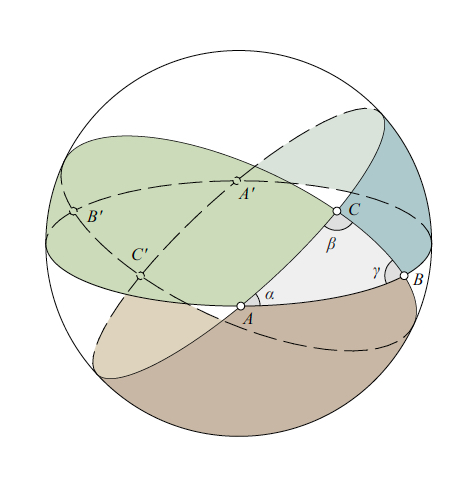
\includegraphics[width=0.4\textwidth]{kugel/Zweiecke.jpg}
    \captionof{figure}{Drei Grosskreise bilden ein sphärisches Dreieck}
\end{center}

In den nachstehenden Erklärungen und Herleitungen, sprechen wir ausschliesslich von Eulerschen’Dreiecken, da die umgeformten Winkelsätze der ebenen Trigonometrie nur auf diese Art von Kugeldreiecken angewendet werden kann.

$A_{ \overline{ ABC }}$ ist die Fläche des Dreieckes auf der Kugeloberfläche
In der ebenen Trigonometrie liegt die Winkelsumme eines Dreiecks bei
$180^{\circ}$.

Anders aber in der sphärischen Trigonometrie. Obschon sie einige Gemeinsamkeiten zur ebenen Trigonometrie aufweist, kann man nicht alles übernehmen.
So auch nicht wie Winkelsumme in einem sphärischen Dreieck.
Diese liegt bei:

\[
\begin{aligned}
\pi
&-
3\pi
&
&\text{\bigg \vert}
&
180^{\circ}
&-
540^{\circ}
\end{aligned}
\]

daraus lässt sich ableiten, das ein einzelner Winkel nicht grösser als $\pi$ oder $180^{\circ}$ sein darf. Ansonsten ist es kein Eulersches’Dreieck und wir dürfen die sphärische Trigonometrie nicht anwenden.\\
Wichtig anzumerken ist, dass die Seiten immer in Radiant beschrieben werden und nicht im Längenmass Meter wie wir es uns gewohnt sind. 
Bei den Dreiecksseiten handelt es sich um Kreisbögen und keine Strecken.

\section{Dreiecksfläche}

\begin{align*}
\text{Zweieck A}
&=
\overline{ABC} + \overline{A'BC} = 2 \alpha r^{ 2 } = A_{ \alpha }\\
\text{Zweieck B}
&=
\overline{ABC} + \overline{AB'C} = 2 \beta r^{ 2 } = A_{ \beta }\\
\text{Zweieck C}
&=
\overline{ABC} + \overline{ABC'} = 2 \gamma r^{ 2 } = A_{ \gamma }
\end{align*}

\begin{align*}
A_{ \alpha } + A_{ \beta } + A_{ \gamma } &= \frac{ 4\pi r^{ 2 } }{ 2 } + 2A_{ \overline{ ABC }} \\
2\alpha r^{ 2 } + 2\beta r^{ 2 } + 2\gamma r^{ 2 } &= \frac{ 4\pi r^{ 2 } }{ 2 } + 2A_{ \overline{ ABC }} \parallel:2\\
\alpha r^{ 2 } + \beta r^{ 2 } + \gamma r^{ 2 } &= \pi r^{ 2 } + A_{ \overline{ ABC }} \parallel-\pi r^{ 2 }\\
r^{ 2 }\left(\alpha + \beta + \gamma - \pi\right) &= A_{ \overline{ ABC }}
\end{align*}




\section{Sphärischer Exzess}
Die Winkelsumme sphärischer Dreiecke ist immer \textgreater \,  $\pi$.

\begin{align*}
\pi < \alpha + \beta + \gamma
\end{align*}

Der sphärische Exzess gibt dabei an, wie stark die Winkelsumme von $\pi$ abweicht.

\begin{align*}
\pi + \epsilon &= \alpha + \beta + \gamma \\
\epsilon &= \alpha + \beta + \gamma - \pi
\end{align*}

Würde der sphärische Exzess in der ebenen Trigonometrie angewendet, wäre dieser = 0. 
Bezieht man das auf die Erde und somit einer Kugel, kann man mit Hilfe eines beliebigen sphärischen Dreieckes und dessen Flächeninhalt auf den Radius der Kugel schliessen.

\subsection{Grenzfall - Satz von Legendre}

\begin{quote} \textit{Ein kleines sphärisches Dreieck kann näherungsweise 
wie ein ebenes Dreieck mit denselben Seiten berechnet 
werden, wenn alle Winkel des ebenen Dreiecks die um 
je ein Drittel des sphärischen Exzesses verminderten 
Winkel des sphärischen Dreiecks nimmt.} \end{quote}
\begin{flushright} - Adrien-Marie Legendre (1752-1833), Paris 1787
\end{flushright}x

Diese Aussage zeigt den Zusammenhang zwischen der 
Trigonometrie in der Ebene sowie in auf der Kugel
auf. Im speziellen bei sehr kleinen sphärischen 
Dreiecken ist die Winkelsumme nur unwesentlich 
grösser als $180^{\circ}$. Des Weiteren kann gesagt werden,
dass der sphärische Exzess gleichmässig auf alle
Winkel aufgeteilt wird.
Wichtig anzumerken ist, dass der Satz von Legendre 
für grosse, aber endliche Radien $r$ gilt.

%[SKIZZE GROSSER RADIUS/KLEINE KRÜMMUNG, KLEINER RADIUS/GROSSE KRÜMMUNG!!!!]
%


\section{Sphärisch Analoge Winkelfunktionen}

\subsection{Sphärischer Sinussatz}

Wir stellen die allgemeinen Sinussätze der Winkel $\alpha$ und $\gamma$ auf:


\[
\begin{aligned}
&{sin(\gamma)} = \frac{h}{a}
&
&\text{\bigg \vert}
&
&{sin(\alpha)} = \frac{h}{c}
&
\end{aligned}
\]

Daraus folgt:
\begin{align*}
h &= sin(\gamma)\cdot a \\
h &= sin(\alpha)\cdot c
\end{align*} 

Durch Gleichsetzung erhält man:
\begin{align*}
h &= h \\
sin(\gamma)\cdot a &= sin(\alpha)\cdot c
\end{align*} 

Durch umstellen erhalten wir den Sinussatz für a und c:
\begin{align*}
sin(\gamma)\cdot a &= sin(\alpha)\cdot c \\
\frac{sin(\gamma)}{c} &= \frac{sin(\alpha)}{a} 
\end{align*} 



\begin{align*}
\frac{sin(\alpha)}{sin(a)} = \frac{sin(\beta)}{sin(b)} = \frac{sin(\gamma)}{sin(c)}
\end{align*} 


\subsection{Winkelkosinussatz}

%[SKIZZE WINKELKOSINUS]

\[
\begin{aligned}
&\overline{C'A'} &= d\cdot {tan(b)}
&
&
&
&
&
&\overline{C'B'} &= d\cdot {tan(a)}
\end{aligned}
\]

\[
\begin{aligned}
&\overline{MA'} &= \frac{ d }{cos(b)}
&
&
&
&
&
&\overline{MB'} &= \frac{ d }{cos(a)}
\end{aligned}
\]

Der allgemeine Kosinussatz beschreibt sich wie folgt:

\begin{align*}
c^{ 2 } &= a^{ 2 } + b^{ 2 } - 2ab \cdot cos(\gamma)
\end{align*}

\begin{align*}
\triangle \overline{A'B'C' }
\overline{ A'B' }^{ 2 } &= \overline{ C'B' }^{ 2 } + \overline{ C'A' }^{ 2 } - 2 \cdot \overline{ C'B' } \cdot \overline{ C'A' } \cdot cos(\gamma)
\end{align*}



\begin{align*}
\overline{A'B'}^{ 2 } &= (d\cdot tan(a))^{ 2 } + (d\cdot tan(b))^{ 2 } - 2 \cdot (d\cdot tan(a) \cdot (d\cdot tan(b) \cdot cos(\gamma)\\
\overline{A'B'}^{ 2 } &= d^{ 2 } \cdot \left(\left(tan^{ 2 }(a) + tan^{ 2 }(b)\right) - 2\cdot tan(a) \cdot tan(b) \cdot cos(\gamma)\right)
\end{align*}

\begin{align*}
\triangle \overline{ MA'B' }
\overline{ A'B' }^{ 2 } &= \overline{ MB' }^{ 2 } + \overline{ MA' }^{ 2 } - 2\cdot \overline{ MB'} \cdot \overline{ MA' } \cdot cos(c)
\end{align*}


\begin{align*}
\overline{ A'B'}^{ 2 } &= \left(\frac{ d }{ cos(a) }  \right)^{ 2 } + \left(\frac{ d }{ cos(b)}  \right)^{ 2 } - 2 \cdot \frac{ d }{ cos(a)} \cdot \frac{ d }{ cos(b)} \cdot cos(c) \\
\overline{ A'B' }^{ 2 } &= d^{ 2 } \cdot \left(\left(\frac{ 1 }{ cos(a) }  \right)^{ 2 } + \left(\frac{ 1 }{ cos(b) }  \right)^{ 2 } - 2 \cdot \frac{ 1 }{ cos(a)} \cdot \frac{ 1 }{ cos(b)} \cdot cos(c)\right)\\
\overline{ A'B' }^{ 2 } &= d^{ 2 } \cdot \left(\left(tan^{ 2 }(a) + 1\right) + \left(tan^{ 2 }(b) + 1\right) - \left(2 \cdot \frac{cos(c)}{cos(a) \cdot cos(b)}\right)\right)
\end{align*}



\begin{align*}
\overline{ A'B'}^{ 2 } &= d^{ 2 } \cdot \left(\left(tan^{ 2 }(a) + tan^{ 2 }(b)\right) - 2 \cdot tan(a) \cdot tan(b) \cdot cos(\gamma)\right) \\
\overline{ A'B'}^{ 2 } &= d^{ 2 } \cdot \left(\left(tan^{ 2 }(a) + 1\right) + \left(tan^{ 2 }(b) + 1\right) - \left(2 \cdot \frac{cos(c)}{cos(a) \cdot cos(b)}\right)\right)
\end{align*}

Die anderen Gleichungen des Satzes, erfolgen aus Symmetriegründen.

\subsection{Seitenkosinussatz}
Durch zyklische Vertauschung des Winkelkosinus erhalten wir den Seitenkosinussatz:

\begin{align*}
{cos(a)} &= {cos(b)} \cdot {cos(c)} + {sin(b)} \cdot {sin(c)} \cdot {sin(\alpha)}\\
{cos(b)} &= {cos(a)} \cdot {cos(c)} + {sin(a)} \cdot {sin(c)} \cdot {sin(\beta)}\\
{cos(c)} &= {cos(a)} \cdot {cos(b)} + {sin(a)} \cdot {sin(b)} \cdot {sin(\gamma)}\\
\end{align*}

\section{Navigation auf See}
Das besondere an Seekarten ist die Inhaltliche Ausrichtung. Anders wie Landkarten muss sie Informationen enthalten welche für den Kapitän und seine Besatzung von grosser Bedeutung sind. Vor allem in Küstennähe ist das navigieren eines Schiffes besonders gefährlich. So enthalten Seekarten etwas über Wassertiefen, Bodenbeschaffenheiten, Gezeiten, Küstenlinien, Landzungen und Windrichtungen.
Der Hauptunterschied dabei ist, das auf der Landkarte feste Positionen definiert und aufgezeigt werden, das einzige was sich verändert ist der Reisende selbst. Bei der Seekarte ist das anders, es werden veränderliche Einwirkungen der Natur festgehalten.

Dieser kleine Unterschied zeigt die Notwendigkeit auf, die Position und den Kurs seines Schiffes auf See immer ermitteln zu können.


\section{Geographische Koordinaten}

Nachdem klar war, das die Erde eine Kugel ist, wurde diese in ein Gradnetz aufgeteilt. Dabei wurden die Angaben für eine exakte Ortsbestimmung klar definiert und die bis heute gültigen Koordinaten bestimmt.
Dabei muss man sich nochmals in Erinnerung rufen, dass sich die Erde in 24h einmal um ihre eigene Achse dreht. Nach $360 ^{\circ}$ 
und somit einer vollen Umdrehung, steht sie wieder in ihrer Ursprungsposition und ein neuer Tag beginnt.

Die Koordinaten setzen sich aus folgenden Komponenten zusammen:

\[
\begin{aligned}
&\text{Grad } (^{\circ})
&
&\text{\bigg \vert}
&
&\text{Bogenminuten } (`)
&
&\text{\bigg \vert}
&
&\text{Bogensekunden } (``)
\end{aligned}
\]

Die Erdoberfläche wurde in je 360 Breiten- und Längengrade eingeteilt. Die Breitengrade haben zueinander einen Abstand von 111.31 km, dies entspricht auch dem Abstand der Längengrade am Äquator mit Zunehmender Nähe zu den Polen, nimmt dieser Abstand ab.

\[
\begin{aligned}
&1^{\circ}
&
&\text{\bigg \vert}
&
&4 \text{ Minuten}
&
&\text{\bigg \vert}
&
&111.31\text{ km}
\end{aligned}
\]

Berechnet man nun die Erdumdrehung von 360°, erhält man genau den Erdumfang am Äquator: \begin{align*} 40’074 \text{ km.}\end{align*}

Dabei geben die Bogenminuten und -sekunden dem Standort die gewünschte Exaktheit. Mit den vollständigen Koordinaten lässt sich der Standort auf einer Landkarte exakt bestimmen und einzeichnen.

\subsection{Zeitzonen der Erde}
Wenn man nun die verschiedenen Zeitzonen der Erde betrachtet, macht die Verschiebung von jeweils einer Stunde durchaus Sinn, es lässt sich auf die Längengrade schliessen.
Zwischen den verschiedenen Zeitzonen liegen 15 Längengrade:

\begin{align*}
\text{15 Längengrade à 4 Minuten = 60 Minuten Zeitverschiebung = ca. 1665 km}
\end{align*}

Dabei ist die Zeitzone in welcher Mitte sich der Greenwich Meredian befindet die \textit{Greenwich Mean Time (GMT)} welche bis 1928 als Weltzeit galt. Im Jahr 1972 wurde diese umbenannt in die \textit{Coordinated Universal Time (UTC)} und wir von da an als Weltzeit $\pm$ 0.00 verwendet.


\section{Der Breitengrad}
Die Breitengrade bilden die bereits genannten Kleinkreise auf der Kugeloberfläche. Sie verlaufen in einem Abstand von genau 111 km parallel zum Äquator. Dabei stellt  dieser genau die Mitte zwischen Nord- und Südpol dar und teilt die Erdkugel in zwei gleiche Hälften. Somit wird von nördlicher und südlicher Breite gesprochen, je nach dem auf welcher Halbkugel man sich befindet.

%[SKIZZE DER GEOGRAFISCHEN BREITE ERDKUGEL]

\subsection{Geografische Breite $\phi$}
\begin{definition}
Die geografische Breite eines Standortes ist nichts anderes, als der Winkel am Erdmittelpunkt zwischen der Ebene des Äquators und der Geraden zum Standpunkt auf der Erdoberfläche.
\end{definition}

%[SKIZZE DER GEOGRAFISCHEN BREITE MIT WINKEL]

\subsection{Navigation mit den Breitengraden}
Da der Breitengrad bereits sehr früh ziemlich präzise bestimmt werden könnte, nutzten bereits die Seefahrer um Christoph Kolumbus den Breitengrad zur Navigation ihrer Flotten.
Den dieser lässt sich ziemlich einfach aus dem höchsten Sonnenstand oder einem Fixstern bestimmen. Dabei wird mit einem Jakobsstab\footnote{%
Der Jakobsstab ist ein früheres astronomisches Instrument zur Winkelmessung und wurde vor allem in der Seefahrt verwendet. Er ist in der Nautik der Vorläufer des Sextanten.} (später Sextant\footnote{%
Der Sextant ist ein nautisches Messinstrument zur Winkelmessung von Horizont und Fixstern (Gestirn)}) der Winkel zwischen dem Horizont und dem Fixstern gemessen. Der Winkel welchen man erhält, zieht man von 90° ab und erhält somit die geografische Breite. \\

%[SKIZZE ERMITTLUNG DES BREITENGRADES]

Wenn man sich auf der Nordhalbkugel befindet, ist der Polarstern ein sehr guter Fixstern. Befindet sich ein Schiff nun sehr nahe am Nordpol, steht dieser nahezu senkrecht am Himmelszelt bei $90^{\circ}$. Würde es aber nahe dem Äquator stehen, erscheint dieser am Horizont bei $0^{\circ}$.

\subsection{Korrekturbeiwert}

\section{Der Längengrad}
Die Längengrade bilden die bereits genannten Grosskreise auf der Kugeloberfläche.
Sie schneiden den Äquator im rechten Winkel, haben dort einen Abstand von 111 km zueinander und verbinden die Pole. Anders wie bei der geografischen Breite, ist in der Natur kein Längengrad gegeben welcher den Nullpunkt darstellt.

%[SKIZZE DER GEOGRAFISCHEN LÄNGE ERDKUGEL]

\subsection{Geografische Länge $\lambda$}
\begin{definition}
Die geografische Länge ist der Winkel an der Erdachse zum Nullmeridian.
\end{definition}

\subsection{Navigation mit den Längengraden}
Die geografische Länge lässt sich nicht so einfach bestimmen wie deren Breite. Für die Berechnung auf See benötigt man eine Referenzzeit eines Ortes mit bekannter Länge.
In der Zeit der Entdecker gab es noch keine mechanischen Uhren. Die Sonnenuhr war zudem ungeeignet, da diese nur die Uhrzeit am Standort mass und nicht die am Referenzort selbst. Die erste Pendeluhr wurde erst Mitte des 17. Jahrhunderts erfunden, was in der Schifffahrt aber auch nicht die Lösung brachte.\\
Pendeluhren auf einem Schiff sind ungeeignet, da das Pendel mit dem Wellengang aus dem Takt gebracht wird und somit die Uhr falsch geht.
Zu ungenau und gegen äussere Erschütterungen zu empfindlich waren später auch die federgetriebenen Uhren und die Unruh. Dazukamen die verschiedenen Klimazonen welche ein Schiff zu durchqueren hatten. Das Metall zog sich viel zu fest zusammen oder dehnte sich aus, was dazu führte das die Uhr unregelmässig lief.

Das sogenannte „Längenproblem“ stellte nicht nur bei der Navigation auf See ein Problem dar, es ergaben sich auch wirtschaftliche Konsequenzen. Die Schiffe mussten bis zur gewünschten geografischen Breite navigieren und segelten dann den Breitengrad entlang. Dabei waren die Schiffe oft Wochenlang unterwegs und segelten die „Breiten ab“ um an die gewünschte Position zu kommen. Dies führte zu erheblichen Zeitverlusten und viel längeren Reisezeiten.


\section{The Board of Longitude - Das Längenproblem}
Das Längenproblem beschäftigte alle grossen Seefahrernationen Europas. Wenn man bedenkt das sich Werte in einer  Höhe von halben britischen Staatshaushalten auf verloren gegangenen Schiffen befanden, erkennt man die Dringlichkeit für eine zuverlässige und genaue Navigation auf See.


\begin{itemize}
\item £ 20’000 - Abweichung von max. einem halben Grad
\item £ 15’000 - Abweichung von zwei Drittel Grad
\item £ 10’000 - Abweichung von max. $1 ^{\circ}$
\end{itemize}

\subsection{John Harrison}


\subsection{Tobias Mayer}



Uhren mit einer Abweichung von einer Minute Abweichung pro Tag (





\section{Nautische Dreieck}


$\Rightarrow$





\section{Die Vermessung der Welt}
Wir schreiben das Jahr 1818 und kehren in die Zeit des Mathematikers Carl Friedrich Gauss zurück. Neben dem liebevoll genannten „kleinen Gauss“ und anderen herausragenden Mathematischen Leistungen, beschäftigte er in den Folgejahren mit der Vermessung des Königreichs Hannovers und verfasste auf 61 Blättern das Kartenwerk \textit{Gauss’sche Landesaufnahme der 1815 durch Hannover erworbenen Gebiete}.






AUFGABE

Hubble Teleskop 
24. April 1990






\printbibliography[heading=subbibliography]
\end{refsection}




%\chapter{Geometrie auf der Kugeloberfläche\label{chapter:kugel}}
\lhead{Geometrie auf der Kugeloberfläche}
\begin{refsection}
\chapterauthor{Melina Staub und Fabian Schmid}

\section{Einleitung}

Schon seit jeher fasziniert den Menschen die Fahrt zur See. Nicht grundlos ist die Seefahrt eine der wichtigsten und ältesten Tätigkeiten der Menschheit. Der innerliche Drang neue Weltmeere und unbekannte Gebiete zu entdecken, die Fahrt zur See zu erleichtern und erträglicher zu machen, trieben die Menschen an, die Schiffe dieser Welt immer weiter zu entwickeln.

Die Idee der Kugelform der Erde ist älter als man zu denken vermag. Bereits der Schüler des antiken griechischen Philosophen Platon - Aristoteles schrieb in seiner Schrift \textit{Über den Himmel} aus dem 4. Jahrhundert v. Chr. etliche Gründe welche für die Gestallt der Erde als Kugel sprechen:

\begin{itemize}
      \item Sämtliche schweren Körper streben zum Mittelpunkt des Alls. Da sie dies von allen Seiten her gleichmäßig tun und die Erde im Mittelpunkt des Alls steht, muss sie eine kugelrunde Gestalt annehmen. 
\item Bei von der Küste wegfahrende Schiffen wird der Rumpf vor den Segeln der Sicht verborgen. 
\item In südlichen Ländern erscheinen südliche Sternbilder höher über dem Horizont.
\item Der Erdschatten bei einer Mondfinsternis ist stets rund.
\end{itemize}

Jedoch war um 1492 - der Zeit der Entdeckung Amerikas durch Christoph Kolumbus, die Idee der Erde in Kugelform noch sehr umstritten. Er erkannte anhand den Theorien und Erkenntnissen der alten Griechen, vor allem Aristoteles, das die Erde eine Kugel sein muss. \\
Doch mit seinem Vorschlag einen Seeweg über den Atlantik nach Indien zu finden und nicht wie üblich um Afrika zu segeln, stiess er beim beim portugiesischen König auf taube Ohren. Sein Plan Indien über eine Route nach Westen zu erreichen, widersprach dem gesunden Menschenverstand. Wäre die Erde wirklich eine Kugel und man befände sich auf der unteren Erdhalbkugel, würde man herunterfallen.\\
Doch auch der damals übliche Glaube an die Erde in Scheibenform brachte so einige Risiken mit sich. Was würde passieren, wenn die Flotte das Ende der Scheibe erreicht hatte? Würden sie über den Erdrand hinweggleiten und in den Abgrund stürzen?\\
Erst nach viel Überzeugungsarbeit durch Kolumbus, setzte er sich am Spanischen Hof durch und segelte über die Westliche Route über den Atlantik und entdeckte schlussendlich Amerika.

Der praktische und greifbare Beweis das die Erde eine Kugel ist, lieferte rund 30 Jahre später der Portugiese Fernando Magellan. Mit seiner Weltumsegelung und seiner Ankunft in den Philippinen, bewies er definitiv das die Erde eine Kugel ist.\\

Nun wollen wir uns die Frage stellen, wie die alten Seefahrer ohne GPS und jeglichen modernen Navigationssystemen auf hoher See wussten wo sie sich befinden und was haben die Sterne mit alldem zu tun? Reisen Sie mit uns zurück in eine Zeit mit Sextant, Kompass und Sternkarten. In die Zeit der Seefahrer und Entdecker.


\section{Geometrie auf der Ebene und der Kugel}

Euklid von Alexandria beschrieb die Grundbegriffe der ebenen Geometrie mittels Punkt, Geraden, Ebene, Winkel und Dreieck. Diese Dreiecke lassen sich mithilfe der ebenen Trigonometrie beschreiben. Dabei gelten die uns bekannten trigonometrischen Winkelfunktionen:\\

\text{Sinussatz:}
\begin{align*}
\frac{ a }{ sin(\alpha) } &= \frac{ b }{sin(\beta)} = \frac{ c }{ sin(\gamma) } = \frac{abc}{2A} = 2r\\
\end{align*}

\text{Cosinussatz:}
\begin{align*}
c^{ 2 } &= a^{ 2 } + b^{ 2 } - 2ab\cdot cos(\gamma)\\
b^{ 2 } &= a^{ 2 } + c^{ 2 } - 2ab\cdot cos(\beta)\\
a^{ 2 } &= b^{ 2 } + c^{ 2 } - 2ab\cdot cos(\alpha)
\end{align*}

Um Dreiecke auf der Kugeloberfläche zu berechnen, benötigt man die sphärische Trigonometrie. Die oben beschriebenen Sätze lassen sich auf der Kugel nicht anwenden, sie werden aber als Grundlage zur Herleitung der Sätze für das Kugeldreieck benötigt.

Die nachfolgenden Seiten thematisieren die Geometrie auf der Kugeloberfläche und wie sie in der Navigation eingesetzt werden kann.


\section{Gross- und Kleinkreise}

Eine Kugeloberfläche lässt sich in zwei verschiedene Kreisarten einteilen -  Gross- und Kleinkreise. 
Wir betrachten als erstes die Grosskreise:

\begin{definition}
Ein Großkreis ist ein größtmöglicher Kreis auf einer Kugeloberfläche. Sein Mittelpunkt fällt immer mit dem Mittelpunkt der Kugel zusammen und ein Schnitt auf dem Großkreis teilt die Kugel in jedem Fall in zwei („gleich große“) Hälften.
\end{definition}

Es gibt unendlich viele Möglichkeiten, eine Kugel in zwei gleich grosse Stücke zu zerschneiden, 
daher gibt es auch unendlich viele Grosskreise. Wenn wir die Grosskreise auf einer Kugel mit diesen auf der Erde beschreiben, sprechen wir von den Längengraden aber auch der Äquator beschreibt einen Grosskreis.
Ein Elementarer Bestandteil bilden die Grosskreise in der sphärischen Trigonometrie. Mithilfe der Schnittpunkte verschiedener Grosskreise, lässt sich ein Sphärisches Dreieck bilden auf welchem sich die sphärische Trigonometrie anwenden lässt.

[GRAFIK GROSSKREISE]

\begin{definition}
Unter Kleinkreis versteht man jene Kreise auf einer Kugeloberfläche, deren Ebenen nicht den Kugelmittelpunkt enthalten.
\end{definition}

Die Kleinkreise eignen sich im Gegensatz zu den Grosskreisen \textit{nicht} für die sphärische Trigonometrie. 
Sie werden lediglich zur Bestimmung der Messgrössen, Winkelabstände oder des Höhenwinkels eines Gestirns verwendet. 

Wenn wir die Kleinkreise auf die Erdoberfläche projizieren betrachten wir die Breitengrade.

[GRAFIK KLEINKREISE]


\section{Sphärische Dreiecke / Kugeldreieck}

\begin{center}
        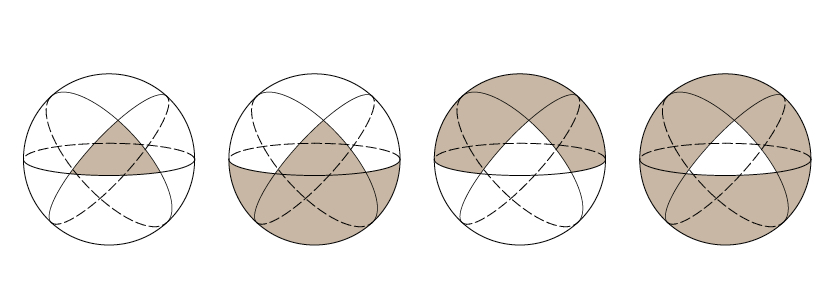
\includegraphics[width=0.9\textwidth]{kugel/Dreieckarten.jpg}
    \captionof{figure}{Dreieckarten auf einer Kugeloberfläche}
\end{center}

Der Begriff Sphärisches Dreieck oder Kugeldreieck ist ein sehr weitläufiger Begriff. 
Dabei können wir den Begriff in drei für uns wesentliche Dreiecke unterteilen:

\begin{itemize}
\item Kugelzweieck
\item Nicht Eulersche’Dreiecke
\item Eulersche’Dreiecke
\end{itemize}

\subsection{Kugelzweieck}

Zwei Grosskreise auf der Kugeloberfläche, zerlegen diese in vier gleiche Kugelzweiecke. 
Jedes dieser Dreieckseiten hat die Länge
$180^{\circ}$ oder $\pi$
Der Flächeninhalt wird dabei nur durch den Winkel $\alpha$ zwischen den beiden Grosskreisen bestimmt.

\begin{center}
        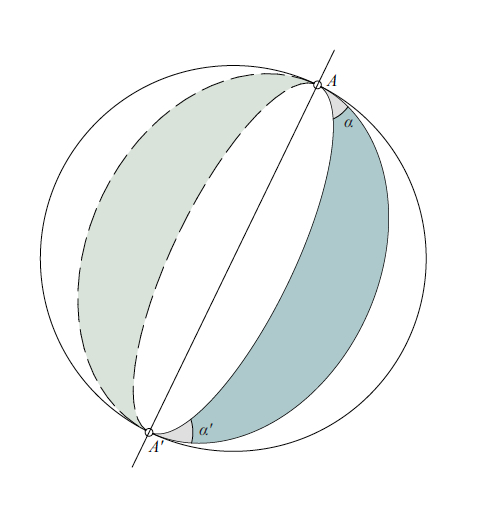
\includegraphics[width=0.3\textwidth]{kugel/Zweieck.jpg}
    \captionof{figure}{Bildung von Zweiecken durch Grosskreise}
\end{center}

Dabei ist der Flächeninhalt der ganzen Kugel:

\begin{align*}
A_{ Kugel } &= 4 \pi r^{2}
\end{align*}


Um den Flächeninhalt des betrachteten Zweieckes zu bekommen, 
müssen wir das ganze noch mit dem Kugelsegment mit dem Winkel $\alpha$ multiplizieren.

\begin{align*}
A_{ Zweieck } &= 4 \pi r^{2} \cdot \frac{ \alpha }{ 2 \pi }
\end{align*}


\subsection{Nicht Eulersche’ Dreiecke}

BLABLA

\subsection{Eulersche’ Dreiecke}

Legt man drei Grosskreise auf eine Kugeloberfläche, bilden sich dabei acht Dreiecke. 
Ein solches Dreieck heisst Eulersches’Dreieck\footnote{%
Leonard Euler (1707-1783), berühmter Schweizer Mathematiker und Physiker. 
Nicht Eulersche’Dreiecke erhält man, indem man das Äussere des Dreieckes ABC betrachtet.} 
Diese Dreiecke werden weder durch die Verlängerung ihrer Seiten durchschnitten, 
noch haben sie Dreiecksseiten welche grösser als $180^{\circ}$ sind.

\begin{center}
        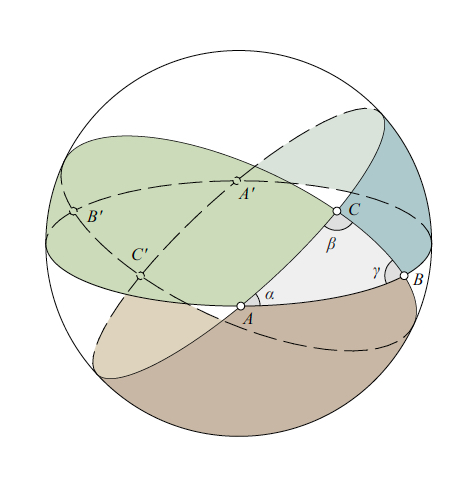
\includegraphics[width=0.4\textwidth]{kugel/Zweiecke.jpg}
    \captionof{figure}{Drei Grosskreise bilden ein sphärisches Dreieck}
\end{center}

In den nachstehenden Erklärungen und Herleitungen, sprechen wir ausschliesslich von Eulerschen’Dreiecken, da die umgeformten Winkelsätze der ebenen Trigonometrie nur auf diese Art von Kugeldreiecken angewendet werden kann.

$A_{ \overline{ ABC }}$ ist die Fläche des Dreieckes auf der Kugeloberfläche
In der ebenen Trigonometrie liegt die Winkelsumme eines Dreiecks bei
$180^{\circ}$.

Anders aber in der sphärischen Trigonometrie. Obschon sie einige Gemeinsamkeiten zur ebenen Trigonometrie aufweist, kann man nicht alles übernehmen.
So auch nicht wie Winkelsumme in einem sphärischen Dreieck.
Diese liegt bei:

\[
\begin{aligned}
\pi
&-
3\pi
&
&\text{\bigg \vert}
&
180^{\circ}
&-
540^{\circ}
\end{aligned}
\]

daraus lässt sich ableiten, das ein einzelner Winkel nicht grösser als $\pi$ oder $180^{\circ}$ sein darf. Ansonsten ist es kein Eulersches’Dreieck und wir dürfen die sphärische Trigonometrie nicht anwenden.\\
Wichtig anzumerken ist, dass die Seiten immer in Radiant beschrieben werden und nicht im Längenmass Meter wie wir es uns gewohnt sind. 
Bei den Dreiecksseiten handelt es sich um Kreisbögen und keine Strecken.

\section{Dreiecksfläche}

\begin{align*}
\text{Zweieck A}
&=
\overline{ABC} + \overline{A'BC} = 2 \alpha r^{ 2 } = A_{ \alpha }\\
\text{Zweieck B}
&=
\overline{ABC} + \overline{AB'C} = 2 \beta r^{ 2 } = A_{ \beta }\\
\text{Zweieck C}
&=
\overline{ABC} + \overline{ABC'} = 2 \gamma r^{ 2 } = A_{ \gamma }
\end{align*}

\begin{align*}
A_{ \alpha } + A_{ \beta } + A_{ \gamma } &= \frac{ 4\pi r^{ 2 } }{ 2 } + 2A_{ \overline{ ABC }} \\
2\alpha r^{ 2 } + 2\beta r^{ 2 } + 2\gamma r^{ 2 } &= \frac{ 4\pi r^{ 2 } }{ 2 } + 2A_{ \overline{ ABC }} \parallel:2\\
\alpha r^{ 2 } + \beta r^{ 2 } + \gamma r^{ 2 } &= \pi r^{ 2 } + A_{ \overline{ ABC }} \parallel-\pi r^{ 2 }\\
r^{ 2 }\left(\alpha + \beta + \gamma - \pi\right) &= A_{ \overline{ ABC }}
\end{align*}




\section{Sphärischer Exzess}
Die Winkelsumme sphärischer Dreiecke ist immer \textgreater \,  $\pi$.

\begin{align*}
\pi < \alpha + \beta + \gamma
\end{align*}

Der sphärische Exzess gibt dabei an, wie stark die Winkelsumme von $\pi$ abweicht.

\begin{align*}
\pi + \epsilon &= \alpha + \beta + \gamma \\
\epsilon &= \alpha + \beta + \gamma - \pi
\end{align*}

Würde der sphärische Exzess in der ebenen Trigonometrie angewendet, wäre dieser = 0. 
Bezieht man das auf die Erde und somit einer Kugel, kann man mit Hilfe eines beliebigen sphärischen Dreieckes und dessen Flächeninhalt auf den Radius der Kugel schliessen.

\subsection{Grenzfall - Satz von Legendre}

\begin{quote} \textit{Ein kleines sphärisches Dreieck kann näherungsweise 
wie ein ebenes Dreieck mit denselben Seiten berechnet 
werden, wenn alle Winkel des ebenen Dreiecks die um 
je ein Drittel des sphärischen Exzesses verminderten 
Winkel des sphärischen Dreiecks nimmt.} \end{quote}
\begin{flushright} - Adrien-Marie Legendre (1752-1833), Paris 1787
\end{flushright}x

Diese Aussage zeigt den Zusammenhang zwischen der 
Trigonometrie in der Ebene sowie in auf der Kugel
auf. Im speziellen bei sehr kleinen sphärischen 
Dreiecken ist die Winkelsumme nur unwesentlich 
grösser als $180^{\circ}$. Des Weiteren kann gesagt werden,
dass der sphärische Exzess gleichmässig auf alle
Winkel aufgeteilt wird.
Wichtig anzumerken ist, dass der Satz von Legendre 
für grosse, aber endliche Radien $r$ gilt.

%[SKIZZE GROSSER RADIUS/KLEINE KRÜMMUNG, KLEINER RADIUS/GROSSE KRÜMMUNG!!!!]
%


\section{Sphärisch Analoge Winkelfunktionen}

\subsection{Sphärischer Sinussatz}

Wir stellen die allgemeinen Sinussätze der Winkel $\alpha$ und $\gamma$ auf:


\[
\begin{aligned}
&{sin(\gamma)} = \frac{h}{a}
&
&\text{\bigg \vert}
&
&{sin(\alpha)} = \frac{h}{c}
&
\end{aligned}
\]

Daraus folgt:
\begin{align*}
h &= sin(\gamma)\cdot a \\
h &= sin(\alpha)\cdot c
\end{align*} 

Durch Gleichsetzung erhält man:
\begin{align*}
h &= h \\
sin(\gamma)\cdot a &= sin(\alpha)\cdot c
\end{align*} 

Durch umstellen erhalten wir den Sinussatz für a und c:
\begin{align*}
sin(\gamma)\cdot a &= sin(\alpha)\cdot c \\
\frac{sin(\gamma)}{c} &= \frac{sin(\alpha)}{a} 
\end{align*} 



\begin{align*}
\frac{sin(\alpha)}{sin(a)} = \frac{sin(\beta)}{sin(b)} = \frac{sin(\gamma)}{sin(c)}
\end{align*} 


\subsection{Winkelkosinussatz}

%[SKIZZE WINKELKOSINUS]

\[
\begin{aligned}
&\overline{C'A'} &= d\cdot {tan(b)}
&
&
&
&
&
&\overline{C'B'} &= d\cdot {tan(a)}
\end{aligned}
\]

\[
\begin{aligned}
&\overline{MA'} &= \frac{ d }{cos(b)}
&
&
&
&
&
&\overline{MB'} &= \frac{ d }{cos(a)}
\end{aligned}
\]

Der allgemeine Kosinussatz beschreibt sich wie folgt:

\begin{align*}
c^{ 2 } &= a^{ 2 } + b^{ 2 } - 2ab \cdot cos(\gamma)
\end{align*}

\begin{align*}
\triangle \overline{A'B'C' }
\overline{ A'B' }^{ 2 } &= \overline{ C'B' }^{ 2 } + \overline{ C'A' }^{ 2 } - 2 \cdot \overline{ C'B' } \cdot \overline{ C'A' } \cdot cos(\gamma)
\end{align*}



\begin{align*}
\overline{A'B'}^{ 2 } &= (d\cdot tan(a))^{ 2 } + (d\cdot tan(b))^{ 2 } - 2 \cdot (d\cdot tan(a) \cdot (d\cdot tan(b) \cdot cos(\gamma)\\
\overline{A'B'}^{ 2 } &= d^{ 2 } \cdot \left(\left(tan^{ 2 }(a) + tan^{ 2 }(b)\right) - 2\cdot tan(a) \cdot tan(b) \cdot cos(\gamma)\right)
\end{align*}

\begin{align*}
\triangle \overline{ MA'B' }
\overline{ A'B' }^{ 2 } &= \overline{ MB' }^{ 2 } + \overline{ MA' }^{ 2 } - 2\cdot \overline{ MB'} \cdot \overline{ MA' } \cdot cos(c)
\end{align*}


\begin{align*}
\overline{ A'B'}^{ 2 } &= \left(\frac{ d }{ cos(a) }  \right)^{ 2 } + \left(\frac{ d }{ cos(b)}  \right)^{ 2 } - 2 \cdot \frac{ d }{ cos(a)} \cdot \frac{ d }{ cos(b)} \cdot cos(c) \\
\overline{ A'B' }^{ 2 } &= d^{ 2 } \cdot \left(\left(\frac{ 1 }{ cos(a) }  \right)^{ 2 } + \left(\frac{ 1 }{ cos(b) }  \right)^{ 2 } - 2 \cdot \frac{ 1 }{ cos(a)} \cdot \frac{ 1 }{ cos(b)} \cdot cos(c)\right)\\
\overline{ A'B' }^{ 2 } &= d^{ 2 } \cdot \left(\left(tan^{ 2 }(a) + 1\right) + \left(tan^{ 2 }(b) + 1\right) - \left(2 \cdot \frac{cos(c)}{cos(a) \cdot cos(b)}\right)\right)
\end{align*}



\begin{align*}
\overline{ A'B'}^{ 2 } &= d^{ 2 } \cdot \left(\left(tan^{ 2 }(a) + tan^{ 2 }(b)\right) - 2 \cdot tan(a) \cdot tan(b) \cdot cos(\gamma)\right) \\
\overline{ A'B'}^{ 2 } &= d^{ 2 } \cdot \left(\left(tan^{ 2 }(a) + 1\right) + \left(tan^{ 2 }(b) + 1\right) - \left(2 \cdot \frac{cos(c)}{cos(a) \cdot cos(b)}\right)\right)
\end{align*}

Die anderen Gleichungen des Satzes, erfolgen aus Symmetriegründen.

\subsection{Seitenkosinussatz}
Durch zyklische Vertauschung des Winkelkosinus erhalten wir den Seitenkosinussatz:

\begin{align*}
{cos(a)} &= {cos(b)} \cdot {cos(c)} + {sin(b)} \cdot {sin(c)} \cdot {sin(\alpha)}\\
{cos(b)} &= {cos(a)} \cdot {cos(c)} + {sin(a)} \cdot {sin(c)} \cdot {sin(\beta)}\\
{cos(c)} &= {cos(a)} \cdot {cos(b)} + {sin(a)} \cdot {sin(b)} \cdot {sin(\gamma)}\\
\end{align*}

\section{Navigation auf See}
Das besondere an Seekarten ist die Inhaltliche Ausrichtung. Anders wie Landkarten muss sie Informationen enthalten welche für den Kapitän und seine Besatzung von grosser Bedeutung sind. Vor allem in Küstennähe ist das navigieren eines Schiffes besonders gefährlich. So enthalten Seekarten etwas über Wassertiefen, Bodenbeschaffenheiten, Gezeiten, Küstenlinien, Landzungen und Windrichtungen.
Der Hauptunterschied dabei ist, das auf der Landkarte feste Positionen definiert und aufgezeigt werden, das einzige was sich verändert ist der Reisende selbst. Bei der Seekarte ist das anders, es werden veränderliche Einwirkungen der Natur festgehalten.

Dieser kleine Unterschied zeigt die Notwendigkeit auf, die Position und den Kurs seines Schiffes auf See immer ermitteln zu können.


\section{Geographische Koordinaten}

Nachdem klar war, das die Erde eine Kugel ist, wurde diese in ein Gradnetz aufgeteilt. Dabei wurden die Angaben für eine exakte Ortsbestimmung klar definiert und die bis heute gültigen Koordinaten bestimmt.
Dabei muss man sich nochmals in Erinnerung rufen, dass sich die Erde in 24h einmal um ihre eigene Achse dreht. Nach $360 ^{\circ}$ 
und somit einer vollen Umdrehung, steht sie wieder in ihrer Ursprungsposition und ein neuer Tag beginnt.

Die Koordinaten setzen sich aus folgenden Komponenten zusammen:

\[
\begin{aligned}
&\text{Grad } (^{\circ})
&
&\text{\bigg \vert}
&
&\text{Bogenminuten } (`)
&
&\text{\bigg \vert}
&
&\text{Bogensekunden } (``)
\end{aligned}
\]

Die Erdoberfläche wurde in je 360 Breiten- und Längengrade eingeteilt. Die Breitengrade haben zueinander einen Abstand von 111.31 km, dies entspricht auch dem Abstand der Längengrade am Äquator mit Zunehmender Nähe zu den Polen, nimmt dieser Abstand ab.

\[
\begin{aligned}
&1^{\circ}
&
&\text{\bigg \vert}
&
&4 \text{ Minuten}
&
&\text{\bigg \vert}
&
&111.31\text{ km}
\end{aligned}
\]

Berechnet man nun die Erdumdrehung von 360°, erhält man genau den Erdumfang am Äquator: \begin{align*} 40’074 \text{ km.}\end{align*}

Dabei geben die Bogenminuten und -sekunden dem Standort die gewünschte Exaktheit. Mit den vollständigen Koordinaten lässt sich der Standort auf einer Landkarte exakt bestimmen und einzeichnen.

\subsection{Zeitzonen der Erde}
Wenn man nun die verschiedenen Zeitzonen der Erde betrachtet, macht die Verschiebung von jeweils einer Stunde durchaus Sinn, es lässt sich auf die Längengrade schliessen.
Zwischen den verschiedenen Zeitzonen liegen 15 Längengrade:

\begin{align*}
\text{15 Längengrade à 4 Minuten = 60 Minuten Zeitverschiebung = ca. 1665 km}
\end{align*}

Dabei ist die Zeitzone in welcher Mitte sich der Greenwich Meredian befindet die \textit{Greenwich Mean Time (GMT)} welche bis 1928 als Weltzeit galt. Im Jahr 1972 wurde diese umbenannt in die \textit{Coordinated Universal Time (UTC)} und wir von da an als Weltzeit $\pm$ 0.00 verwendet.


\section{Der Breitengrad}
Die Breitengrade bilden die bereits genannten Kleinkreise auf der Kugeloberfläche. Sie verlaufen in einem Abstand von genau 111 km parallel zum Äquator. Dabei stellt  dieser genau die Mitte zwischen Nord- und Südpol dar und teilt die Erdkugel in zwei gleiche Hälften. Somit wird von nördlicher und südlicher Breite gesprochen, je nach dem auf welcher Halbkugel man sich befindet.

%[SKIZZE DER GEOGRAFISCHEN BREITE ERDKUGEL]

\subsection{Geografische Breite $\phi$}
\begin{definition}
Die geografische Breite eines Standortes ist nichts anderes, als der Winkel am Erdmittelpunkt zwischen der Ebene des Äquators und der Geraden zum Standpunkt auf der Erdoberfläche.
\end{definition}

%[SKIZZE DER GEOGRAFISCHEN BREITE MIT WINKEL]

\subsection{Navigation mit den Breitengraden}
Da der Breitengrad bereits sehr früh ziemlich präzise bestimmt werden könnte, nutzten bereits die Seefahrer um Christoph Kolumbus den Breitengrad zur Navigation ihrer Flotten.
Den dieser lässt sich ziemlich einfach aus dem höchsten Sonnenstand oder einem Fixstern bestimmen. Dabei wird mit einem Jakobsstab\footnote{%
Der Jakobsstab ist ein früheres astronomisches Instrument zur Winkelmessung und wurde vor allem in der Seefahrt verwendet. Er ist in der Nautik der Vorläufer des Sextanten.} (später Sextant\footnote{%
Der Sextant ist ein nautisches Messinstrument zur Winkelmessung von Horizont und Fixstern (Gestirn)}) der Winkel zwischen dem Horizont und dem Fixstern gemessen. Der Winkel welchen man erhält, zieht man von 90° ab und erhält somit die geografische Breite. \\

%[SKIZZE ERMITTLUNG DES BREITENGRADES]

Wenn man sich auf der Nordhalbkugel befindet, ist der Polarstern ein sehr guter Fixstern. Befindet sich ein Schiff nun sehr nahe am Nordpol, steht dieser nahezu senkrecht am Himmelszelt bei $90^{\circ}$. Würde es aber nahe dem Äquator stehen, erscheint dieser am Horizont bei $0^{\circ}$.

\subsection{Korrekturbeiwert}

\section{Der Längengrad}
Die Längengrade bilden die bereits genannten Grosskreise auf der Kugeloberfläche.
Sie schneiden den Äquator im rechten Winkel, haben dort einen Abstand von 111 km zueinander und verbinden die Pole. Anders wie bei der geografischen Breite, ist in der Natur kein Längengrad gegeben welcher den Nullpunkt darstellt.

%[SKIZZE DER GEOGRAFISCHEN LÄNGE ERDKUGEL]

\subsection{Geografische Länge $\lambda$}
\begin{definition}
Die geografische Länge ist der Winkel an der Erdachse zum Nullmeridian.
\end{definition}

\subsection{Navigation mit den Längengraden}
Die geografische Länge lässt sich nicht so einfach bestimmen wie deren Breite. Für die Berechnung auf See benötigt man eine Referenzzeit eines Ortes mit bekannter Länge.
In der Zeit der Entdecker gab es noch keine mechanischen Uhren. Die Sonnenuhr war zudem ungeeignet, da diese nur die Uhrzeit am Standort mass und nicht die am Referenzort selbst. Die erste Pendeluhr wurde erst Mitte des 17. Jahrhunderts erfunden, was in der Schifffahrt aber auch nicht die Lösung brachte.\\
Pendeluhren auf einem Schiff sind ungeeignet, da das Pendel mit dem Wellengang aus dem Takt gebracht wird und somit die Uhr falsch geht.
Zu ungenau und gegen äussere Erschütterungen zu empfindlich waren später auch die federgetriebenen Uhren und die Unruh. Dazukamen die verschiedenen Klimazonen welche ein Schiff zu durchqueren hatten. Das Metall zog sich viel zu fest zusammen oder dehnte sich aus, was dazu führte das die Uhr unregelmässig lief.

Das sogenannte „Längenproblem“ stellte nicht nur bei der Navigation auf See ein Problem dar, es ergaben sich auch wirtschaftliche Konsequenzen. Die Schiffe mussten bis zur gewünschten geografischen Breite navigieren und segelten dann den Breitengrad entlang. Dabei waren die Schiffe oft Wochenlang unterwegs und segelten die „Breiten ab“ um an die gewünschte Position zu kommen. Dies führte zu erheblichen Zeitverlusten und viel längeren Reisezeiten.


\section{The Board of Longitude - Das Längenproblem}
Das Längenproblem beschäftigte alle grossen Seefahrernationen Europas. Wenn man bedenkt das sich Werte in einer  Höhe von halben britischen Staatshaushalten auf verloren gegangenen Schiffen befanden, erkennt man die Dringlichkeit für eine zuverlässige und genaue Navigation auf See.


\begin{itemize}
\item £ 20’000 - Abweichung von max. einem halben Grad
\item £ 15’000 - Abweichung von zwei Drittel Grad
\item £ 10’000 - Abweichung von max. $1 ^{\circ}$
\end{itemize}

\subsection{John Harrison}


\subsection{Tobias Mayer}



Uhren mit einer Abweichung von einer Minute Abweichung pro Tag (





\section{Nautische Dreieck}


$\Rightarrow$





\section{Die Vermessung der Welt}
Wir schreiben das Jahr 1818 und kehren in die Zeit des Mathematikers Carl Friedrich Gauss zurück. Neben dem liebevoll genannten „kleinen Gauss“ und anderen herausragenden Mathematischen Leistungen, beschäftigte er in den Folgejahren mit der Vermessung des Königreichs Hannovers und verfasste auf 61 Blättern das Kartenwerk \textit{Gauss’sche Landesaufnahme der 1815 durch Hannover erworbenen Gebiete}.






AUFGABE

Hubble Teleskop 
24. April 1990






\printbibliography[heading=subbibliography]
\end{refsection}




\vfill
\pagebreak
\ifodd\value{page}\else\null\clearpage\fi
\lhead{Index}
\rhead{}
\addcontentsline{toc}{chapter}{\indexname}
%
% skript.tex -- Skript ueber Differentialgleichungen
%
% (c) 2014 Prof. Dr. Andreas Mueller, HSR
%
\documentclass{book}
\usepackage{etex}
\usepackage{geometry}
\geometry{papersize={170mm,240mm},total={140mm,200mm},top=21mm,bindingoffset=10mm}
\usepackage[english,ngerman]{babel}
\usepackage[utf8]{inputenc}
\usepackage{cancel}
\usepackage{times}
\usepackage{amsmath,amscd}
\usepackage{amssymb}
\usepackage{amsfonts}
\usepackage{amsthm}
\usepackage[nolist]{acronym}
\usepackage{graphicx}
\usepackage{fancyhdr}
\usepackage{textcomp}
\usepackage[all]{xy}
\usepackage{txfonts}
\usepackage{alltt} 
\usepackage{verbatim}
\usepackage{paralist}
\usepackage{makeidx}
\usepackage{array}
%\usepackage[colorlinks=true]{hyperref}
\usepackage{hyperref}
\usepackage{tikz}
\usepackage{pgfplots}
\usepackage{pgfplotstable}
\usepackage{pdftexcmds}
%\usepackage{pgfmath}
\usepackage{placeins}
\usepackage{subfigure}
\usepackage[autostyle=false,english=american]{csquotes}
\usepackage{float}
\usepackage{enumitem}
\usepackage{wasysym}
\usepackage{environ}
\usepackage{pifont}
\usepackage{feynmp}
\usepackage{appendix}
\usetikzlibrary{calc,intersections,through,backgrounds,graphs,positioning,shapes,arrows,fit}
\usetikzlibrary{patterns,decorations.pathreplacing}
\usetikzlibrary{decorations.pathreplacing}
\usetikzlibrary{external}
\usepackage[europeanvoltages,
            europeancurrents,
            europeanresistors,   % rectangular shape
            americaninductors,   % "4-bumbs" shape
            europeanports,       % rectangular logic ports
            siunitx,             % #1<#2>
            emptydiodes,
            noarrowmos,
            smartlabels]         % lables are rotated in a smart way
           {circuitikz}          %
\usepackage{siunitx}
\usepackage{tabularx}
\usetikzlibrary{arrows}

\usepackage{algpseudocode}
\usepackage{algorithm}

% Matlab
\usepackage{listings}
\usepackage{color} %red, green, blue, yellow, cyan, magenta, black, white
\definecolor{mygreen}{RGB}{28,172,0} % color values Red, Green, Blue
\definecolor{mylilas}{RGB}{170,55,241}

\lstset{language=Matlab,%
    %basicstyle=\color{red},
    breaklines=true,%
    morekeywords={matlab2tikz},
    keywordstyle=\color{blue},%
    morekeywords=[2]{1}, keywordstyle=[2]{\color{black}},
    identifierstyle=\color{black},%
    stringstyle=\color{mylilas},
    commentstyle=\color{mygreen},%
    showstringspaces=false,%without this there will be a symbol in the places where there is a space
    numbers=left,%
    %numberstyle={\tiny \color{black}},% size of the numbers
    numbersep=9pt, % this defines how far the numbers are from the text
    emph=[1]{break},emphstyle=[1]\color{red}, %some words to emphasise
    %emph=[2]{word1,word2}, emphstyle=[2]{style},    
}
\lstdefinestyle{Matlab}{
  numbers=left,
  belowcaptionskip=1\baselineskip,
  breaklines=true,
  frame=L,
  xleftmargin=\parindent,
  language=Matlab,
  showstringspaces=false,
  basicstyle=\footnotesize\ttfamily,
  keywordstyle=\bfseries\color{green!40!black},
  commentstyle=\itshape\color{purple!40!black},
  identifierstyle=\color{blue},
  stringstyle=\color{orange},
  numberstyle=\ttfamily\tiny
}
\lstdefinelanguage{Maxima}{
  keywords={addrow,addcol,zeromatrix,ident,augcoefmatrix,ratsubst,sum,diff,ev,tex,%
    with_stdout,nouns,express,depends,load,length,submatrix,div,grad,curl,matrix,%
    invert,lambda,facsum,expand,false,then,if,else,subst,%
    rootscontract,solve,part,assume,sqrt,integrate,abs,inf,exp,sin,cos,sinh,cosh},
  sensitive=true,
  comment=[n][\itshape]{/*}{*/}
}
\lstdefinestyle{Maxima}{
  numbers=left,
  belowcaptionskip=1\baselineskip,
  breaklines=true,
  frame=L,
  xleftmargin=\parindent,
  language=Maxima,
  showstringspaces=false,
  basicstyle=\footnotesize\ttfamily,
  keywordstyle=\bfseries\color{green!40!black},
  commentstyle=\itshape\color{purple!40!black},
  identifierstyle=\color{blue},
  stringstyle=\color{orange},
  numberstyle=\ttfamily\tiny
}
\lstdefinestyle{Octave}{
  numbers=left,
  belowcaptionskip=1\baselineskip,
  breaklines=true,
  frame=L,
  xleftmargin=\parindent,
  language=Octave,
  showstringspaces=false,
  basicstyle=\footnotesize\ttfamily,
  keywordstyle=\bfseries\color{green!40!black},
  commentstyle=\itshape\color{purple!40!black},
  identifierstyle=\color{blue},
  stringstyle=\color{orange},
  numberstyle=\ttfamily\tiny
}
\lstdefinestyle{C}{
  numbers=left,
  belowcaptionskip=1\baselineskip,
  breaklines=true,
  frame=L,
  xleftmargin=\parindent,
  language=C,
  showstringspaces=false,
  basicstyle=\footnotesize\ttfamily,
  keywordstyle=\bfseries\color{green!40!black},
  commentstyle=\itshape\color{purple!40!black},
  identifierstyle=\color{blue},
  stringstyle=\color{orange},
  numberstyle=\ttfamily\tiny
}
\usepackage{caption}
\usepackage[mode=buildnew]{standalone}
\usepackage[backend=bibtex]{biblatex}
% workaround for biblatex bug
\makeatletter
\def\blx@maxline{77}
\makeatother
\addbibresource{references.bib}
% Bibresources für jeden einzelnen Artikel
%\addbibresource{friedmann/main.bib}
%\addbibresource{komplex/main.bib}
%\addbibresource{kreis/main.bib}
%\addbibresource{licht/main.bib}
%\addbibresource{schrittlaenge/main.bib}
%\addbibresource{sir/main.bib}
%\addbibresource{trafo/main.bib}
%\addbibresource{wellen/main.bib}
\AtEndDocument{\clearpage\ifodd\value{page}\else\null\clearpage\fi}
\makeindex
%\pgfplotsset{compat=1.12}
\setlength{\headheight}{15pt} % fix headheight warning
\DeclareGraphicsRule{*}{mps}{*}{}
\begin{document}
\pagestyle{fancy}
\frontmatter
\newcommand\HRule{\noindent\rule{\linewidth}{1.5pt}}
\begin{titlepage}
\vspace*{\stretch{1}}
\HRule
\vspace*{5pt}
\begin{flushright}
{
\LARGE
Mathematisches Seminar\\
\vspace*{20pt}
\Huge
Kosmologie%
}
\vspace*{5pt}
\end{flushright}
\HRule
\begin{flushright}
\vspace{60pt}
\Large
Leitung: Andreas M"uller\\
\vspace{40pt}
\Large
%Reto~Christen,
%Kevin~Cina,
%Andri~Hartmann,
%Pascal~Horat %,
%Matthias~Kn"opfel,
%Stefan Kull,
%Daniela~Meier,
%Max~Obrist %,
%Hansruedi~Patzen,
%Benjamin~R"aber,
%Simon~Schaefer %,
%Tibor~Schneider,
%Tobias~Schuler,
%Roy~Seitz,
%Martin~Stypinski
\end{flushright}
\vspace*{\stretch{2}}
\begin{center}
Hochschule f"ur Technik, Rapperswil, 2017
\end{center}
\end{titlepage}
\hypersetup{
    linktoc=all,
    linkcolor=blue
}
\newcounter{beispiel}
\newenvironment{beispiele}{
\bgroup\smallskip\parindent0pt\bf Beispiele\egroup

\begin{list}{\arabic{beispiel}.}
  {\usecounter{beispiel}
  \setlength{\labelsep}{5mm}
  \setlength{\rightmargin}{0pt}
}}{\end{list}}
\newcounter{uebungsaufgabezaehler}
% environment fuer uebungsaufgaben
\newenvironment{uebungsaufgaben}{
\begin{list}{\arabic{uebungsaufgabezaehler}.}
  {\usecounter{uebungsaufgabezaehler}
  \setlength{\labelwidth}{2cm}
  \setlength{\leftmargin}{0pt}
  \setlength{\labelsep}{5mm}
  \setlength{\rightmargin}{0pt}
  \setlength{\itemindent}{0pt}
}}{\end{list}\vfill\pagebreak}
\newenvironment{teilaufgaben}{
\begin{enumerate}
\renewcommand{\labelenumi}{\alph{enumi})}
}{\end{enumerate}}
% Aufgabe
\newcounter{problemcounter}[chapter]
\def\aufgabepath{uebungsaufgaben/}
\def\ainput#1{\input\aufgabepath/#1}
\def\verbatimainput#1{\expandafter\verbatiminput{\aufgabepath/#1}}
\def\aufgabetoplevel#1{%
\expandafter\def\expandafter\inputpath{#1}%
\let\aufgabepath=\inputpath
}
\def\includeagraphics[#1]#2{\expandafter\includegraphics[#1]{\aufgabepath#2}}
% \aufgabe
\newcommand{\uebungsaufgabe}[1]{%
\refstepcounter{problemcounter}%
\label{#1}%
\bigskip{\parindent0pt\strut}\hbox{\bf\arabic{problemcounter}. }%
\expandafter\def\csname aufgabepath\endcsname{\inputpath/}%
\expandafter\input{uebungsaufgaben/#1.tex}
}
\renewcommand\theproblemcounter{\thechapter.\arabic{problemcounter}}

% Loesung
\def\swallow#1{
%nothing
}
\NewEnviron{loesung}[1][L"osung]{%
\begin{proof}[#1]%
\renewcommand{\qedsymbol}{$\bigcirc$}
\BODY
\end{proof}
}
\NewEnviron{bewertung}{%
\begin{proof}[Bewertung]%
\renewcommand{\qedsymbol}{}
\BODY
\end{proof}
}
\NewEnviron{diskussion}{%
\begin{proof}[Diskussion]%
\renewcommand{\qedsymbol}{}
\BODY
\end{proof}
}
\NewEnviron{hinweis}{%
\begin{proof}[Hinweis]%
\renewcommand{\qedsymbol}{}
\BODY
\end{proof}
}
\def\keineloesungen{%
\RenewEnviron{loesung}{\relax}
\RenewEnviron{bewertung}{\relax}
\RenewEnviron{diskussion}{\relax}
}
\newenvironment{beispiel}{%
\begin{proof}[Beispiel]%
\renewcommand{\qedsymbol}{$\bigcirc$}
}{\end{proof}}

%%%%%%%%%%%%%%%%%%%%%%%
%% Copyleft
%% Walter A. Kehowski
%% Department of Mathematics
%% Glendale Community College
%% walter.kehowski@gcmail.maricopa.edu
%% \begin{linsys}{2}
%% -x & + & 4y & = & 8\\
%% -3x & - & 2y & = & 6
%% \end{linsys}
%%%%%%%%%%%%%%%%%%%%%%%
%\makeatletter
%% math-mode column types ------------------
\newcolumntype{\linsysR}{>{$}r<{$}}
\newcolumntype{\linsysL}{>{$}l<{$}}
\newcolumntype{\linsysC}{>{$}c<{$}}
\newenvironment{linsys}[1]{%
\begin{tabular}{*{#1}{\linsysR@{\;}\linsysC}@{\;}\linsysR}}%
{\end{tabular}}
%\makeatother
\endinput

\allowdisplaybreaks

\lhead{Inhaltsverzeichnis}
\rhead{}
\tableofcontents
\newtheorem{satz}{Satz}[chapter]
\newtheorem{hilfssatz}[satz]{Hilfssatz}
\newtheorem{definition}[satz]{Definition}
\newtheorem{annahme}[satz]{Annahme}
\newtheorem{problem}[satz]{Problem}
\newtheorem*{problem*}{Problem}
\renewcommand{\floatpagefraction}{0.75}
\mainmatter
%
% vorwort.tex -- Vorwort zum Buch zum Seminar
%
% (c) 2015 Prof Dr Andreas Mueller, Hochschule Rapperswil
%
\chapter*{Vorwort}
\lhead{Vorwort}
\rhead{}
Dieses Buch entstand im Rahmen des Mathematischen Seminars
im Frühjahrssemester 2017 an der Hochschule für Technik Rapperswil.
Die Teilnehmer, Studierende der Abteilungen für Elektrotechnik,
Informatik und Bauingenieurwesen der
HSR, erarbeiteten nach einer Einführung in das Themengebiet jeweils
einzelne Aspekte des Gebietes in Form einer Seminararbeit, über
deren Resultate sie auch in einem Vortrag informierten. 

Im Frühjahr 2017 war das Thema des Seminars ``Mathematics for
the Universe''.
Es wurden drei mathematische Themengebiete besprochen, die für
das Verständnis des Universums unerlässlich sind, die aber auch
interessante Anwendungen in den Ingenieurwissenschaften haben.
Zur Sprache kam im ersten Thema das Konzept der Krümmung,
welches einerseits zentral für das Verständnis der Entwicklung
des Universums ist, aber auch Methoden für die Behanldung 
zum Beispiel der Geometrie auf gekrümmten Flächen bereitstellt.

Das zweite Thema ging von der für die Elektrotechnik wichtigen
Multipolzerlegung aus.
Daraus wurde dann die Analyse von Funktionen auf einer Kugeloberfläche,
die harmonische Analyse nach Kugelfunktionen entwickelt.
In der Kosmologie leitet man aus einer Analyse des kosmischen
Mikrowellenhintergrundes ab, dass das Universum flach ist.
In der Ingenieurpraxis gibt es Anwendungen dafür zum Beispiel
beim Registrierungsproblem \cite{skript:tabea}.

Das dritte Thema behandelt globale Modelle für das Universum.
Dabei wird eine Technik angewandt, die auch zum Beispiel in der
Strömungsmodellierung erfolgreich ist.
Beim Reynolds-Averaging mittelt man zum Beispiel die Details
der turbulenten Strömung aus und ersetzt die Navier-Stokes-Gleichungen
durch einfacher zu lösende Gleichungen.
Dabei verliert man zwar auch einige Information, aber man gewinnt
ein Modell, das immer noch globale Aussagen über die Strömung
ermöglicht.
Im kosmologischen Zusammenhang kann man ein homogenes und isotropes
Universum mit der Friedmann-Gleichung modellieren.

Die Einführung bestand aus einigen Vorlesungsstunden, deren
Inhalt im ersten Teil dieses Skripts zusammengefasst ist.  

Im zweiten Teil dieses Skripts kommen dann die Teilnehmer selbst zu Wort.
Ihre Arbeiten wurden jeweils als einzelne
Kapitel mit meist nur typographischen Änderungen übernommen.
Diese weiterführenden Kapitel sind sehr verschiedenartig.
Eine Übersicht und Einführung befindet sich in der Einleitung
zum zweiten Teil auf Seite~\pageref{skript:uebersicht}.

In einigen Arbeiten wurde auch Code zur Demonstration der 
besprochenen Methoden und Resultate geschrieben, soweit
möglich und sinnvoll wurde dieser Code im Github-Repository
dieses Kurses\footnote{\url{https://github.com/AndreasFMueller/Seminar17.git}}
abgelegt, in anderen Fällen verweisen die Artikel selbst auf
das zugehörige Code-Repository.

Im genannten Repository findet sich auch der Source-Code dieses
Skriptes, es wird hier unter einer Creative Commons Lizenz
zur Verfügung gestellt.


\part{Grundlagen}
%\keineloesungen
\begin{refsection}
%
% einleitung.tex -- Einleitung zum Skript ueber Differentialgleichungen
%
% (c) 2015 Prof Dr Andreas Mueller, Hochschule Rapperswil
%
\chapter*{Einleitung\label{chapter:einleitung}}
\lhead{Einleitung}
\rhead{}


%
% kruemmung.tex
%
% (c) 2017 Prof Dr Andreas Müller, Hochschule Rapperswil
%
\chapter{Krümmung\label{skript:chapter:kruemmung}}
\lhead{Krümmung}
\rhead{}


%
% multipol.tex
%
% (c) 2017 Prof Dr Andreas Müller, Hochschule Rapperswil
%
\chapter{Multipolentwicklung, Kugelfunktionen und der
kosmische Mikrowellenhintergrund
\label{skript:chapter:multipol}}
\lhead{Multipole und CMB}
\rhead{}


%
% friedmann.tex
%
% (c) 2017 Prof Dr Andreas Müller, Hochschule Rapperswil
%
\chapter{Modellgleichungen\label{skript:chapter:modellgleichungen}}
\lhead{Modellgleichungen}
\rhead{}
Natürliche Systeme sind meistens so komplex, dass es praktisch nicht
möglich ist, jedes einzelne Detail physikalisch exakt wiederzugeben.
Es ist daher notwendig, vereinfachte Modelle zu verwenden, welche 
die Anzahl der zu berücksichtigenden Variablen reduzieren auf eine
Art, die immer noch gestattet, die gestellten Fragen mit ausreichender
Genauigkeit zu beantworten.

In diesem Kapitel betrachten wir zunächst ein paar Beispiele aus den
Naturwissenschaften, welche diesen Prozess der Modellbildung exemplarisch
vorstellen.
Anschliessend wird ein Modell für das Universum betrachtet, welches
das Universum derart vereinfacht, dass über die langfristige
Geschichte des Universums konkrete Aussagen zu machen gestattet.
Mit diesen sogenannten Friedmann-Gleichungen kann man sodann zum
Beispiel das Alter des Universums bestimmen.

\input{chapters/f-beispiele.tex}
\input{chapters/f-friedmann.tex}




%\input{kapitel.tex}
\begin{appendices}
%\input{chapters/newton.tex}
%\input{chapters/komplexezahlen.tex}
\end{appendices}
\vfill
\pagebreak
\ifodd\value{page}\else\null\clearpage\fi
\lhead{Literatur}
\rhead{}
\printbibliography[heading=subbibliography]
\label{skript:literatur}
\end{refsection}

\part{Anwendungen und Weiterf"uhrende Themen}
\lhead{Anwendungen}
%
% uebersicht.tex -- Uebersicht ueber die Seminar-Arbeiten
%
% (c) 2015 Prof Dr Andreas Mueller, Hochschule Rapperswil
%
\chapter*{"Ubersicht}
\lhead{"Ubersicht}
\rhead{}
\label{skript:uebersicht}
Im zweiten Teil kommen die Teilnehmer des Seminars selbst zu Wort.
Sie zeigen Anwendungsbeispiele f"ur die im ersten
Teil entwickelte Theorie der gew"ohnlichen Differentialgleichungen.
Eine breite Vielfalt von Arbeiten vertieft einzelne Aspekte der Theorie,
untersucht spezielle Differentialgleichungen im Detail
oder erm"oglicht das bessere Verst"andnis interessanter Anwendungen.

%{\em Daniela Meier} und {\em Hansruedi Patzen} untersuchen eine spezielle
%Differentialgleichung zweiter Ordnung mit Hilfe der Potenzreihenmethode
%und entwickeln einiges an Intuition, wie L"osungen einer solchen Gleichung
%aussehen m"ussen.
%Sie decken auch Schwierigkeiten bei der numerischen Berechnung der
%Potenzreihenl"osung auf.
%
%{\em Kevin Cina} und {\em Benjamin R"aber} untersuchen das zylindersymmetrische
%Wellenausbreitungsproblem, leiten die Besselsche Differentialgleichung
%her, und l"osen sie mit Hilfe eines Potenzreihenansatz.
%Sie finden so die Besselfunktionen, ausser im Falle $\nu =0$.
%Diesen Fall untersuche {\em Stefan Kull} und {\em Roy Seitz}, sie konstruieren
%die mit dem reinen Potenzreihenansatz nicht zug"angliche zweite linear
%unabh"angige L"osung.
%Ihre Darstellung verwendet einen originellen Operator zur Formalisierung
%der analytische Fortsetzung.
%
%{\em Pascal Horat} und {\em Matthias Kn"opfel} untersuchen das Problem
%der Schrittl"ange bei der numerischen L"osung gew"ohnlicher
%Differentialgleichung.
%Aus den Lehren an einem Beispielproblem leiten sie einen eigenen
%Schrittl"angensteuerungsalgorithmus ab und untersuchen seine Leistung.
%
%{\em Simon Sch"afer} und {\em Tibor Schneider} entwickeln die
%Differentialgleichungen f"ur die Lichtbrechung in der Atmosph"are, und
%simulieren sie f"ur verschiedene Atmosph"arenmodelle.
%Eine weitere Anwendung untersuchen {\em Max Obrist} und {\em Martin Stypinski}.
%Sie modellieren die Ausbreitung anste\discretionary{k-}{k}{ck}ender Krankheiten, und erweitern
%ihr Modell auch auf die bevorstehende Zombie-Apokalypse.
%
%{\em Andri Hartmann} und {\em Tobias Schuler} untersuchen die 
%Friedmann-Gleichung, die die Expansion des Universums seit dem
%Urknall beschreibt.
%Sie wurden urspr"unglich
%durch Lema\^{i}tre und Friedmann
%als L"osungen der Feldgleichungen
%der allgemeinen Relativit"atstheorie von Albert Einstein
%entdeckt.
%Es wird eine Motivation der Gleichungen gegeben sowie eine
%ausf"uhrliche Diskussion der verschiedenen Szenarien durchgef"uhrt.
%
%Als abschliessendes Beispiel zeigt {\em Reto Christen}, wie ein Transformator
%simuliert werden kann. 
%Seine L"osung zeichnet sich durch besonders hohe Rechengeschwindigkeit aus,
%welche dank eines vertieften Verst"andnisses der Mathematik des Problems
%erreicht werden konnte.
%
%
%
%
%
%
%
%
%
%
%

\def\chapterauthor#1{{\large #1}\bigskip\bigskip}
% Artikel
%\chapter{Geometrie auf der Kugeloberfläche\label{chapter:kugel}}
\lhead{Geometrie auf der Kugeloberfläche}
\begin{refsection}
\chapterauthor{Melina Staub und Fabian Schmid}

\section{Einleitung}

Schon seit jeher fasziniert den Menschen die Fahrt zur See. Nicht grundlos ist die Seefahrt eine der wichtigsten und ältesten Tätigkeiten der Menschheit. Der innerliche Drang neue Weltmeere und unbekannte Gebiete zu entdecken, die Fahrt zur See zu erleichtern und erträglicher zu machen, trieben die Menschen an, die Schiffe dieser Welt immer weiter zu entwickeln.

Die Idee der Kugelform der Erde ist älter als man zu denken vermag. Bereits der Schüler des antiken griechischen Philosophen Platon - Aristoteles schrieb in seiner Schrift \textit{Über den Himmel} aus dem 4. Jahrhundert v. Chr. etliche Gründe welche für die Gestallt der Erde als Kugel sprechen:

\begin{itemize}
      \item Sämtliche schweren Körper streben zum Mittelpunkt des Alls. Da sie dies von allen Seiten her gleichmäßig tun und die Erde im Mittelpunkt des Alls steht, muss sie eine kugelrunde Gestalt annehmen. 
\item Bei von der Küste wegfahrende Schiffen wird der Rumpf vor den Segeln der Sicht verborgen. 
\item In südlichen Ländern erscheinen südliche Sternbilder höher über dem Horizont.
\item Der Erdschatten bei einer Mondfinsternis ist stets rund.
\end{itemize}

Jedoch war um 1492 - der Zeit der Entdeckung Amerikas durch Christoph Kolumbus, die Idee der Erde in Kugelform noch sehr umstritten. Er erkannte anhand den Theorien und Erkenntnissen der alten Griechen, vor allem Aristoteles, das die Erde eine Kugel sein muss. \\
Doch mit seinem Vorschlag einen Seeweg über den Atlantik nach Indien zu finden und nicht wie üblich um Afrika zu segeln, stiess er beim beim portugiesischen König auf taube Ohren. Sein Plan Indien über eine Route nach Westen zu erreichen, widersprach dem gesunden Menschenverstand. Wäre die Erde wirklich eine Kugel und man befände sich auf der unteren Erdhalbkugel, würde man herunterfallen.\\
Doch auch der damals übliche Glaube an die Erde in Scheibenform brachte so einige Risiken mit sich. Was würde passieren, wenn die Flotte das Ende der Scheibe erreicht hatte? Würden sie über den Erdrand hinweggleiten und in den Abgrund stürzen?\\
Erst nach viel Überzeugungsarbeit durch Kolumbus, setzte er sich am Spanischen Hof durch und segelte über die Westliche Route über den Atlantik und entdeckte schlussendlich Amerika.

Der praktische und greifbare Beweis das die Erde eine Kugel ist, lieferte rund 30 Jahre später der Portugiese Fernando Magellan. Mit seiner Weltumsegelung und seiner Ankunft in den Philippinen, bewies er definitiv das die Erde eine Kugel ist.\\

Nun wollen wir uns die Frage stellen, wie die alten Seefahrer ohne GPS und jeglichen modernen Navigationssystemen auf hoher See wussten wo sie sich befinden und was haben die Sterne mit alldem zu tun? Reisen Sie mit uns zurück in eine Zeit mit Sextant, Kompass und Sternkarten. In die Zeit der Seefahrer und Entdecker.


\section{Geometrie auf der Ebene und der Kugel}

Euklid von Alexandria beschrieb die Grundbegriffe der ebenen Geometrie mittels Punkt, Geraden, Ebene, Winkel und Dreieck. Diese Dreiecke lassen sich mithilfe der ebenen Trigonometrie beschreiben. Dabei gelten die uns bekannten trigonometrischen Winkelfunktionen:\\

\text{Sinussatz:}
\begin{align*}
\frac{ a }{ sin(\alpha) } &= \frac{ b }{sin(\beta)} = \frac{ c }{ sin(\gamma) } = \frac{abc}{2A} = 2r\\
\end{align*}

\text{Cosinussatz:}
\begin{align*}
c^{ 2 } &= a^{ 2 } + b^{ 2 } - 2ab\cdot cos(\gamma)\\
b^{ 2 } &= a^{ 2 } + c^{ 2 } - 2ab\cdot cos(\beta)\\
a^{ 2 } &= b^{ 2 } + c^{ 2 } - 2ab\cdot cos(\alpha)
\end{align*}

Um Dreiecke auf der Kugeloberfläche zu berechnen, benötigt man die sphärische Trigonometrie. Die oben beschriebenen Sätze lassen sich auf der Kugel nicht anwenden, sie werden aber als Grundlage zur Herleitung der Sätze für das Kugeldreieck benötigt.

Die nachfolgenden Seiten thematisieren die Geometrie auf der Kugeloberfläche und wie sie in der Navigation eingesetzt werden kann.


\section{Gross- und Kleinkreise}

Eine Kugeloberfläche lässt sich in zwei verschiedene Kreisarten einteilen -  Gross- und Kleinkreise. 
Wir betrachten als erstes die Grosskreise:

\begin{definition}
Ein Großkreis ist ein größtmöglicher Kreis auf einer Kugeloberfläche. Sein Mittelpunkt fällt immer mit dem Mittelpunkt der Kugel zusammen und ein Schnitt auf dem Großkreis teilt die Kugel in jedem Fall in zwei („gleich große“) Hälften.
\end{definition}

Es gibt unendlich viele Möglichkeiten, eine Kugel in zwei gleich grosse Stücke zu zerschneiden, 
daher gibt es auch unendlich viele Grosskreise. Wenn wir die Grosskreise auf einer Kugel mit diesen auf der Erde beschreiben, sprechen wir von den Längengraden aber auch der Äquator beschreibt einen Grosskreis.
Ein Elementarer Bestandteil bilden die Grosskreise in der sphärischen Trigonometrie. Mithilfe der Schnittpunkte verschiedener Grosskreise, lässt sich ein Sphärisches Dreieck bilden auf welchem sich die sphärische Trigonometrie anwenden lässt.

[GRAFIK GROSSKREISE]

\begin{definition}
Unter Kleinkreis versteht man jene Kreise auf einer Kugeloberfläche, deren Ebenen nicht den Kugelmittelpunkt enthalten.
\end{definition}

Die Kleinkreise eignen sich im Gegensatz zu den Grosskreisen \textit{nicht} für die sphärische Trigonometrie. 
Sie werden lediglich zur Bestimmung der Messgrössen, Winkelabstände oder des Höhenwinkels eines Gestirns verwendet. 

Wenn wir die Kleinkreise auf die Erdoberfläche projizieren betrachten wir die Breitengrade.

[GRAFIK KLEINKREISE]


\section{Sphärische Dreiecke / Kugeldreieck}

\begin{center}
        \includegraphics[width=0.9\textwidth]{kugel/Dreieckarten.jpg}
    \captionof{figure}{Dreieckarten auf einer Kugeloberfläche}
\end{center}

Der Begriff Sphärisches Dreieck oder Kugeldreieck ist ein sehr weitläufiger Begriff. 
Dabei können wir den Begriff in drei für uns wesentliche Dreiecke unterteilen:

\begin{itemize}
\item Kugelzweieck
\item Nicht Eulersche’Dreiecke
\item Eulersche’Dreiecke
\end{itemize}

\subsection{Kugelzweieck}

Zwei Grosskreise auf der Kugeloberfläche, zerlegen diese in vier gleiche Kugelzweiecke. 
Jedes dieser Dreieckseiten hat die Länge
$180^{\circ}$ oder $\pi$
Der Flächeninhalt wird dabei nur durch den Winkel $\alpha$ zwischen den beiden Grosskreisen bestimmt.

\begin{center}
        \includegraphics[width=0.3\textwidth]{kugel/Zweieck.jpg}
    \captionof{figure}{Bildung von Zweiecken durch Grosskreise}
\end{center}

Dabei ist der Flächeninhalt der ganzen Kugel:

\begin{align*}
A_{ Kugel } &= 4 \pi r^{2}
\end{align*}


Um den Flächeninhalt des betrachteten Zweieckes zu bekommen, 
müssen wir das ganze noch mit dem Kugelsegment mit dem Winkel $\alpha$ multiplizieren.

\begin{align*}
A_{ Zweieck } &= 4 \pi r^{2} \cdot \frac{ \alpha }{ 2 \pi }
\end{align*}


\subsection{Nicht Eulersche’ Dreiecke}

BLABLA

\subsection{Eulersche’ Dreiecke}

Legt man drei Grosskreise auf eine Kugeloberfläche, bilden sich dabei acht Dreiecke. 
Ein solches Dreieck heisst Eulersches’Dreieck\footnote{%
Leonard Euler (1707-1783), berühmter Schweizer Mathematiker und Physiker. 
Nicht Eulersche’Dreiecke erhält man, indem man das Äussere des Dreieckes ABC betrachtet.} 
Diese Dreiecke werden weder durch die Verlängerung ihrer Seiten durchschnitten, 
noch haben sie Dreiecksseiten welche grösser als $180^{\circ}$ sind.

\begin{center}
        \includegraphics[width=0.4\textwidth]{kugel/Zweiecke.jpg}
    \captionof{figure}{Drei Grosskreise bilden ein sphärisches Dreieck}
\end{center}

In den nachstehenden Erklärungen und Herleitungen, sprechen wir ausschliesslich von Eulerschen’Dreiecken, da die umgeformten Winkelsätze der ebenen Trigonometrie nur auf diese Art von Kugeldreiecken angewendet werden kann.

$A_{ \overline{ ABC }}$ ist die Fläche des Dreieckes auf der Kugeloberfläche
In der ebenen Trigonometrie liegt die Winkelsumme eines Dreiecks bei
$180^{\circ}$.

Anders aber in der sphärischen Trigonometrie. Obschon sie einige Gemeinsamkeiten zur ebenen Trigonometrie aufweist, kann man nicht alles übernehmen.
So auch nicht wie Winkelsumme in einem sphärischen Dreieck.
Diese liegt bei:

\[
\begin{aligned}
\pi
&-
3\pi
&
&\text{\bigg \vert}
&
180^{\circ}
&-
540^{\circ}
\end{aligned}
\]

daraus lässt sich ableiten, das ein einzelner Winkel nicht grösser als $\pi$ oder $180^{\circ}$ sein darf. Ansonsten ist es kein Eulersches’Dreieck und wir dürfen die sphärische Trigonometrie nicht anwenden.\\
Wichtig anzumerken ist, dass die Seiten immer in Radiant beschrieben werden und nicht im Längenmass Meter wie wir es uns gewohnt sind. 
Bei den Dreiecksseiten handelt es sich um Kreisbögen und keine Strecken.

\section{Dreiecksfläche}

\begin{align*}
\text{Zweieck A}
&=
\overline{ABC} + \overline{A'BC} = 2 \alpha r^{ 2 } = A_{ \alpha }\\
\text{Zweieck B}
&=
\overline{ABC} + \overline{AB'C} = 2 \beta r^{ 2 } = A_{ \beta }\\
\text{Zweieck C}
&=
\overline{ABC} + \overline{ABC'} = 2 \gamma r^{ 2 } = A_{ \gamma }
\end{align*}

\begin{align*}
A_{ \alpha } + A_{ \beta } + A_{ \gamma } &= \frac{ 4\pi r^{ 2 } }{ 2 } + 2A_{ \overline{ ABC }} \\
2\alpha r^{ 2 } + 2\beta r^{ 2 } + 2\gamma r^{ 2 } &= \frac{ 4\pi r^{ 2 } }{ 2 } + 2A_{ \overline{ ABC }} \parallel:2\\
\alpha r^{ 2 } + \beta r^{ 2 } + \gamma r^{ 2 } &= \pi r^{ 2 } + A_{ \overline{ ABC }} \parallel-\pi r^{ 2 }\\
r^{ 2 }\left(\alpha + \beta + \gamma - \pi\right) &= A_{ \overline{ ABC }}
\end{align*}




\section{Sphärischer Exzess}
Die Winkelsumme sphärischer Dreiecke ist immer \textgreater \,  $\pi$.

\begin{align*}
\pi < \alpha + \beta + \gamma
\end{align*}

Der sphärische Exzess gibt dabei an, wie stark die Winkelsumme von $\pi$ abweicht.

\begin{align*}
\pi + \epsilon &= \alpha + \beta + \gamma \\
\epsilon &= \alpha + \beta + \gamma - \pi
\end{align*}

Würde der sphärische Exzess in der ebenen Trigonometrie angewendet, wäre dieser = 0. 
Bezieht man das auf die Erde und somit einer Kugel, kann man mit Hilfe eines beliebigen sphärischen Dreieckes und dessen Flächeninhalt auf den Radius der Kugel schliessen.

\subsection{Grenzfall - Satz von Legendre}

\begin{quote} \textit{Ein kleines sphärisches Dreieck kann näherungsweise 
wie ein ebenes Dreieck mit denselben Seiten berechnet 
werden, wenn alle Winkel des ebenen Dreiecks die um 
je ein Drittel des sphärischen Exzesses verminderten 
Winkel des sphärischen Dreiecks nimmt.} \end{quote}
\begin{flushright} - Adrien-Marie Legendre (1752-1833), Paris 1787
\end{flushright}x

Diese Aussage zeigt den Zusammenhang zwischen der 
Trigonometrie in der Ebene sowie in auf der Kugel
auf. Im speziellen bei sehr kleinen sphärischen 
Dreiecken ist die Winkelsumme nur unwesentlich 
grösser als $180^{\circ}$. Des Weiteren kann gesagt werden,
dass der sphärische Exzess gleichmässig auf alle
Winkel aufgeteilt wird.
Wichtig anzumerken ist, dass der Satz von Legendre 
für grosse, aber endliche Radien $r$ gilt.

%[SKIZZE GROSSER RADIUS/KLEINE KRÜMMUNG, KLEINER RADIUS/GROSSE KRÜMMUNG!!!!]
%


\section{Sphärisch Analoge Winkelfunktionen}

\subsection{Sphärischer Sinussatz}

Wir stellen die allgemeinen Sinussätze der Winkel $\alpha$ und $\gamma$ auf:


\[
\begin{aligned}
&{sin(\gamma)} = \frac{h}{a}
&
&\text{\bigg \vert}
&
&{sin(\alpha)} = \frac{h}{c}
&
\end{aligned}
\]

Daraus folgt:
\begin{align*}
h &= sin(\gamma)\cdot a \\
h &= sin(\alpha)\cdot c
\end{align*} 

Durch Gleichsetzung erhält man:
\begin{align*}
h &= h \\
sin(\gamma)\cdot a &= sin(\alpha)\cdot c
\end{align*} 

Durch umstellen erhalten wir den Sinussatz für a und c:
\begin{align*}
sin(\gamma)\cdot a &= sin(\alpha)\cdot c \\
\frac{sin(\gamma)}{c} &= \frac{sin(\alpha)}{a} 
\end{align*} 



\begin{align*}
\frac{sin(\alpha)}{sin(a)} = \frac{sin(\beta)}{sin(b)} = \frac{sin(\gamma)}{sin(c)}
\end{align*} 


\subsection{Winkelkosinussatz}

%[SKIZZE WINKELKOSINUS]

\[
\begin{aligned}
&\overline{C'A'} &= d\cdot {tan(b)}
&
&
&
&
&
&\overline{C'B'} &= d\cdot {tan(a)}
\end{aligned}
\]

\[
\begin{aligned}
&\overline{MA'} &= \frac{ d }{cos(b)}
&
&
&
&
&
&\overline{MB'} &= \frac{ d }{cos(a)}
\end{aligned}
\]

Der allgemeine Kosinussatz beschreibt sich wie folgt:

\begin{align*}
c^{ 2 } &= a^{ 2 } + b^{ 2 } - 2ab \cdot cos(\gamma)
\end{align*}

\begin{align*}
\triangle \overline{A'B'C' }
\overline{ A'B' }^{ 2 } &= \overline{ C'B' }^{ 2 } + \overline{ C'A' }^{ 2 } - 2 \cdot \overline{ C'B' } \cdot \overline{ C'A' } \cdot cos(\gamma)
\end{align*}



\begin{align*}
\overline{A'B'}^{ 2 } &= (d\cdot tan(a))^{ 2 } + (d\cdot tan(b))^{ 2 } - 2 \cdot (d\cdot tan(a) \cdot (d\cdot tan(b) \cdot cos(\gamma)\\
\overline{A'B'}^{ 2 } &= d^{ 2 } \cdot \left(\left(tan^{ 2 }(a) + tan^{ 2 }(b)\right) - 2\cdot tan(a) \cdot tan(b) \cdot cos(\gamma)\right)
\end{align*}

\begin{align*}
\triangle \overline{ MA'B' }
\overline{ A'B' }^{ 2 } &= \overline{ MB' }^{ 2 } + \overline{ MA' }^{ 2 } - 2\cdot \overline{ MB'} \cdot \overline{ MA' } \cdot cos(c)
\end{align*}


\begin{align*}
\overline{ A'B'}^{ 2 } &= \left(\frac{ d }{ cos(a) }  \right)^{ 2 } + \left(\frac{ d }{ cos(b)}  \right)^{ 2 } - 2 \cdot \frac{ d }{ cos(a)} \cdot \frac{ d }{ cos(b)} \cdot cos(c) \\
\overline{ A'B' }^{ 2 } &= d^{ 2 } \cdot \left(\left(\frac{ 1 }{ cos(a) }  \right)^{ 2 } + \left(\frac{ 1 }{ cos(b) }  \right)^{ 2 } - 2 \cdot \frac{ 1 }{ cos(a)} \cdot \frac{ 1 }{ cos(b)} \cdot cos(c)\right)\\
\overline{ A'B' }^{ 2 } &= d^{ 2 } \cdot \left(\left(tan^{ 2 }(a) + 1\right) + \left(tan^{ 2 }(b) + 1\right) - \left(2 \cdot \frac{cos(c)}{cos(a) \cdot cos(b)}\right)\right)
\end{align*}



\begin{align*}
\overline{ A'B'}^{ 2 } &= d^{ 2 } \cdot \left(\left(tan^{ 2 }(a) + tan^{ 2 }(b)\right) - 2 \cdot tan(a) \cdot tan(b) \cdot cos(\gamma)\right) \\
\overline{ A'B'}^{ 2 } &= d^{ 2 } \cdot \left(\left(tan^{ 2 }(a) + 1\right) + \left(tan^{ 2 }(b) + 1\right) - \left(2 \cdot \frac{cos(c)}{cos(a) \cdot cos(b)}\right)\right)
\end{align*}

Die anderen Gleichungen des Satzes, erfolgen aus Symmetriegründen.

\subsection{Seitenkosinussatz}
Durch zyklische Vertauschung des Winkelkosinus erhalten wir den Seitenkosinussatz:

\begin{align*}
{cos(a)} &= {cos(b)} \cdot {cos(c)} + {sin(b)} \cdot {sin(c)} \cdot {sin(\alpha)}\\
{cos(b)} &= {cos(a)} \cdot {cos(c)} + {sin(a)} \cdot {sin(c)} \cdot {sin(\beta)}\\
{cos(c)} &= {cos(a)} \cdot {cos(b)} + {sin(a)} \cdot {sin(b)} \cdot {sin(\gamma)}\\
\end{align*}

\section{Navigation auf See}
Das besondere an Seekarten ist die Inhaltliche Ausrichtung. Anders wie Landkarten muss sie Informationen enthalten welche für den Kapitän und seine Besatzung von grosser Bedeutung sind. Vor allem in Küstennähe ist das navigieren eines Schiffes besonders gefährlich. So enthalten Seekarten etwas über Wassertiefen, Bodenbeschaffenheiten, Gezeiten, Küstenlinien, Landzungen und Windrichtungen.
Der Hauptunterschied dabei ist, das auf der Landkarte feste Positionen definiert und aufgezeigt werden, das einzige was sich verändert ist der Reisende selbst. Bei der Seekarte ist das anders, es werden veränderliche Einwirkungen der Natur festgehalten.

Dieser kleine Unterschied zeigt die Notwendigkeit auf, die Position und den Kurs seines Schiffes auf See immer ermitteln zu können.


\section{Geographische Koordinaten}

Nachdem klar war, das die Erde eine Kugel ist, wurde diese in ein Gradnetz aufgeteilt. Dabei wurden die Angaben für eine exakte Ortsbestimmung klar definiert und die bis heute gültigen Koordinaten bestimmt.
Dabei muss man sich nochmals in Erinnerung rufen, dass sich die Erde in 24h einmal um ihre eigene Achse dreht. Nach $360 ^{\circ}$ 
und somit einer vollen Umdrehung, steht sie wieder in ihrer Ursprungsposition und ein neuer Tag beginnt.

Die Koordinaten setzen sich aus folgenden Komponenten zusammen:

\[
\begin{aligned}
&\text{Grad } (^{\circ})
&
&\text{\bigg \vert}
&
&\text{Bogenminuten } (`)
&
&\text{\bigg \vert}
&
&\text{Bogensekunden } (``)
\end{aligned}
\]

Die Erdoberfläche wurde in je 360 Breiten- und Längengrade eingeteilt. Die Breitengrade haben zueinander einen Abstand von 111.31 km, dies entspricht auch dem Abstand der Längengrade am Äquator mit Zunehmender Nähe zu den Polen, nimmt dieser Abstand ab.

\[
\begin{aligned}
&1^{\circ}
&
&\text{\bigg \vert}
&
&4 \text{ Minuten}
&
&\text{\bigg \vert}
&
&111.31\text{ km}
\end{aligned}
\]

Berechnet man nun die Erdumdrehung von 360°, erhält man genau den Erdumfang am Äquator: \begin{align*} 40’074 \text{ km.}\end{align*}

Dabei geben die Bogenminuten und -sekunden dem Standort die gewünschte Exaktheit. Mit den vollständigen Koordinaten lässt sich der Standort auf einer Landkarte exakt bestimmen und einzeichnen.

\subsection{Zeitzonen der Erde}
Wenn man nun die verschiedenen Zeitzonen der Erde betrachtet, macht die Verschiebung von jeweils einer Stunde durchaus Sinn, es lässt sich auf die Längengrade schliessen.
Zwischen den verschiedenen Zeitzonen liegen 15 Längengrade:

\begin{align*}
\text{15 Längengrade à 4 Minuten = 60 Minuten Zeitverschiebung = ca. 1665 km}
\end{align*}

Dabei ist die Zeitzone in welcher Mitte sich der Greenwich Meredian befindet die \textit{Greenwich Mean Time (GMT)} welche bis 1928 als Weltzeit galt. Im Jahr 1972 wurde diese umbenannt in die \textit{Coordinated Universal Time (UTC)} und wir von da an als Weltzeit $\pm$ 0.00 verwendet.


\section{Der Breitengrad}
Die Breitengrade bilden die bereits genannten Kleinkreise auf der Kugeloberfläche. Sie verlaufen in einem Abstand von genau 111 km parallel zum Äquator. Dabei stellt  dieser genau die Mitte zwischen Nord- und Südpol dar und teilt die Erdkugel in zwei gleiche Hälften. Somit wird von nördlicher und südlicher Breite gesprochen, je nach dem auf welcher Halbkugel man sich befindet.

%[SKIZZE DER GEOGRAFISCHEN BREITE ERDKUGEL]

\subsection{Geografische Breite $\phi$}
\begin{definition}
Die geografische Breite eines Standortes ist nichts anderes, als der Winkel am Erdmittelpunkt zwischen der Ebene des Äquators und der Geraden zum Standpunkt auf der Erdoberfläche.
\end{definition}

%[SKIZZE DER GEOGRAFISCHEN BREITE MIT WINKEL]

\subsection{Navigation mit den Breitengraden}
Da der Breitengrad bereits sehr früh ziemlich präzise bestimmt werden könnte, nutzten bereits die Seefahrer um Christoph Kolumbus den Breitengrad zur Navigation ihrer Flotten.
Den dieser lässt sich ziemlich einfach aus dem höchsten Sonnenstand oder einem Fixstern bestimmen. Dabei wird mit einem Jakobsstab\footnote{%
Der Jakobsstab ist ein früheres astronomisches Instrument zur Winkelmessung und wurde vor allem in der Seefahrt verwendet. Er ist in der Nautik der Vorläufer des Sextanten.} (später Sextant\footnote{%
Der Sextant ist ein nautisches Messinstrument zur Winkelmessung von Horizont und Fixstern (Gestirn)}) der Winkel zwischen dem Horizont und dem Fixstern gemessen. Der Winkel welchen man erhält, zieht man von 90° ab und erhält somit die geografische Breite. \\

%[SKIZZE ERMITTLUNG DES BREITENGRADES]

Wenn man sich auf der Nordhalbkugel befindet, ist der Polarstern ein sehr guter Fixstern. Befindet sich ein Schiff nun sehr nahe am Nordpol, steht dieser nahezu senkrecht am Himmelszelt bei $90^{\circ}$. Würde es aber nahe dem Äquator stehen, erscheint dieser am Horizont bei $0^{\circ}$.

\subsection{Korrekturbeiwert}

\section{Der Längengrad}
Die Längengrade bilden die bereits genannten Grosskreise auf der Kugeloberfläche.
Sie schneiden den Äquator im rechten Winkel, haben dort einen Abstand von 111 km zueinander und verbinden die Pole. Anders wie bei der geografischen Breite, ist in der Natur kein Längengrad gegeben welcher den Nullpunkt darstellt.

%[SKIZZE DER GEOGRAFISCHEN LÄNGE ERDKUGEL]

\subsection{Geografische Länge $\lambda$}
\begin{definition}
Die geografische Länge ist der Winkel an der Erdachse zum Nullmeridian.
\end{definition}

\subsection{Navigation mit den Längengraden}
Die geografische Länge lässt sich nicht so einfach bestimmen wie deren Breite. Für die Berechnung auf See benötigt man eine Referenzzeit eines Ortes mit bekannter Länge.
In der Zeit der Entdecker gab es noch keine mechanischen Uhren. Die Sonnenuhr war zudem ungeeignet, da diese nur die Uhrzeit am Standort mass und nicht die am Referenzort selbst. Die erste Pendeluhr wurde erst Mitte des 17. Jahrhunderts erfunden, was in der Schifffahrt aber auch nicht die Lösung brachte.\\
Pendeluhren auf einem Schiff sind ungeeignet, da das Pendel mit dem Wellengang aus dem Takt gebracht wird und somit die Uhr falsch geht.
Zu ungenau und gegen äussere Erschütterungen zu empfindlich waren später auch die federgetriebenen Uhren und die Unruh. Dazukamen die verschiedenen Klimazonen welche ein Schiff zu durchqueren hatten. Das Metall zog sich viel zu fest zusammen oder dehnte sich aus, was dazu führte das die Uhr unregelmässig lief.

Das sogenannte „Längenproblem“ stellte nicht nur bei der Navigation auf See ein Problem dar, es ergaben sich auch wirtschaftliche Konsequenzen. Die Schiffe mussten bis zur gewünschten geografischen Breite navigieren und segelten dann den Breitengrad entlang. Dabei waren die Schiffe oft Wochenlang unterwegs und segelten die „Breiten ab“ um an die gewünschte Position zu kommen. Dies führte zu erheblichen Zeitverlusten und viel längeren Reisezeiten.


\section{The Board of Longitude - Das Längenproblem}
Das Längenproblem beschäftigte alle grossen Seefahrernationen Europas. Wenn man bedenkt das sich Werte in einer  Höhe von halben britischen Staatshaushalten auf verloren gegangenen Schiffen befanden, erkennt man die Dringlichkeit für eine zuverlässige und genaue Navigation auf See.


\begin{itemize}
\item £ 20’000 - Abweichung von max. einem halben Grad
\item £ 15’000 - Abweichung von zwei Drittel Grad
\item £ 10’000 - Abweichung von max. $1 ^{\circ}$
\end{itemize}

\subsection{John Harrison}


\subsection{Tobias Mayer}



Uhren mit einer Abweichung von einer Minute Abweichung pro Tag (





\section{Nautische Dreieck}


$\Rightarrow$





\section{Die Vermessung der Welt}
Wir schreiben das Jahr 1818 und kehren in die Zeit des Mathematikers Carl Friedrich Gauss zurück. Neben dem liebevoll genannten „kleinen Gauss“ und anderen herausragenden Mathematischen Leistungen, beschäftigte er in den Folgejahren mit der Vermessung des Königreichs Hannovers und verfasste auf 61 Blättern das Kartenwerk \textit{Gauss’sche Landesaufnahme der 1815 durch Hannover erworbenen Gebiete}.






AUFGABE

Hubble Teleskop 
24. April 1990






\printbibliography[heading=subbibliography]
\end{refsection}




%\chapter{Geometrie auf der Kugeloberfläche\label{chapter:kugel}}
\lhead{Geometrie auf der Kugeloberfläche}
\begin{refsection}
\chapterauthor{Melina Staub und Fabian Schmid}

\section{Einleitung}

Schon seit jeher fasziniert den Menschen die Fahrt zur See. Nicht grundlos ist die Seefahrt eine der wichtigsten und ältesten Tätigkeiten der Menschheit. Der innerliche Drang neue Weltmeere und unbekannte Gebiete zu entdecken, die Fahrt zur See zu erleichtern und erträglicher zu machen, trieben die Menschen an, die Schiffe dieser Welt immer weiter zu entwickeln.

Die Idee der Kugelform der Erde ist älter als man zu denken vermag. Bereits der Schüler des antiken griechischen Philosophen Platon - Aristoteles schrieb in seiner Schrift \textit{Über den Himmel} aus dem 4. Jahrhundert v. Chr. etliche Gründe welche für die Gestallt der Erde als Kugel sprechen:

\begin{itemize}
      \item Sämtliche schweren Körper streben zum Mittelpunkt des Alls. Da sie dies von allen Seiten her gleichmäßig tun und die Erde im Mittelpunkt des Alls steht, muss sie eine kugelrunde Gestalt annehmen. 
\item Bei von der Küste wegfahrende Schiffen wird der Rumpf vor den Segeln der Sicht verborgen. 
\item In südlichen Ländern erscheinen südliche Sternbilder höher über dem Horizont.
\item Der Erdschatten bei einer Mondfinsternis ist stets rund.
\end{itemize}

Jedoch war um 1492 - der Zeit der Entdeckung Amerikas durch Christoph Kolumbus, die Idee der Erde in Kugelform noch sehr umstritten. Er erkannte anhand den Theorien und Erkenntnissen der alten Griechen, vor allem Aristoteles, das die Erde eine Kugel sein muss. \\
Doch mit seinem Vorschlag einen Seeweg über den Atlantik nach Indien zu finden und nicht wie üblich um Afrika zu segeln, stiess er beim beim portugiesischen König auf taube Ohren. Sein Plan Indien über eine Route nach Westen zu erreichen, widersprach dem gesunden Menschenverstand. Wäre die Erde wirklich eine Kugel und man befände sich auf der unteren Erdhalbkugel, würde man herunterfallen.\\
Doch auch der damals übliche Glaube an die Erde in Scheibenform brachte so einige Risiken mit sich. Was würde passieren, wenn die Flotte das Ende der Scheibe erreicht hatte? Würden sie über den Erdrand hinweggleiten und in den Abgrund stürzen?\\
Erst nach viel Überzeugungsarbeit durch Kolumbus, setzte er sich am Spanischen Hof durch und segelte über die Westliche Route über den Atlantik und entdeckte schlussendlich Amerika.

Der praktische und greifbare Beweis das die Erde eine Kugel ist, lieferte rund 30 Jahre später der Portugiese Fernando Magellan. Mit seiner Weltumsegelung und seiner Ankunft in den Philippinen, bewies er definitiv das die Erde eine Kugel ist.\\

Nun wollen wir uns die Frage stellen, wie die alten Seefahrer ohne GPS und jeglichen modernen Navigationssystemen auf hoher See wussten wo sie sich befinden und was haben die Sterne mit alldem zu tun? Reisen Sie mit uns zurück in eine Zeit mit Sextant, Kompass und Sternkarten. In die Zeit der Seefahrer und Entdecker.


\section{Geometrie auf der Ebene und der Kugel}

Euklid von Alexandria beschrieb die Grundbegriffe der ebenen Geometrie mittels Punkt, Geraden, Ebene, Winkel und Dreieck. Diese Dreiecke lassen sich mithilfe der ebenen Trigonometrie beschreiben. Dabei gelten die uns bekannten trigonometrischen Winkelfunktionen:\\

\text{Sinussatz:}
\begin{align*}
\frac{ a }{ sin(\alpha) } &= \frac{ b }{sin(\beta)} = \frac{ c }{ sin(\gamma) } = \frac{abc}{2A} = 2r\\
\end{align*}

\text{Cosinussatz:}
\begin{align*}
c^{ 2 } &= a^{ 2 } + b^{ 2 } - 2ab\cdot cos(\gamma)\\
b^{ 2 } &= a^{ 2 } + c^{ 2 } - 2ab\cdot cos(\beta)\\
a^{ 2 } &= b^{ 2 } + c^{ 2 } - 2ab\cdot cos(\alpha)
\end{align*}

Um Dreiecke auf der Kugeloberfläche zu berechnen, benötigt man die sphärische Trigonometrie. Die oben beschriebenen Sätze lassen sich auf der Kugel nicht anwenden, sie werden aber als Grundlage zur Herleitung der Sätze für das Kugeldreieck benötigt.

Die nachfolgenden Seiten thematisieren die Geometrie auf der Kugeloberfläche und wie sie in der Navigation eingesetzt werden kann.


\section{Gross- und Kleinkreise}

Eine Kugeloberfläche lässt sich in zwei verschiedene Kreisarten einteilen -  Gross- und Kleinkreise. 
Wir betrachten als erstes die Grosskreise:

\begin{definition}
Ein Großkreis ist ein größtmöglicher Kreis auf einer Kugeloberfläche. Sein Mittelpunkt fällt immer mit dem Mittelpunkt der Kugel zusammen und ein Schnitt auf dem Großkreis teilt die Kugel in jedem Fall in zwei („gleich große“) Hälften.
\end{definition}

Es gibt unendlich viele Möglichkeiten, eine Kugel in zwei gleich grosse Stücke zu zerschneiden, 
daher gibt es auch unendlich viele Grosskreise. Wenn wir die Grosskreise auf einer Kugel mit diesen auf der Erde beschreiben, sprechen wir von den Längengraden aber auch der Äquator beschreibt einen Grosskreis.
Ein Elementarer Bestandteil bilden die Grosskreise in der sphärischen Trigonometrie. Mithilfe der Schnittpunkte verschiedener Grosskreise, lässt sich ein Sphärisches Dreieck bilden auf welchem sich die sphärische Trigonometrie anwenden lässt.

[GRAFIK GROSSKREISE]

\begin{definition}
Unter Kleinkreis versteht man jene Kreise auf einer Kugeloberfläche, deren Ebenen nicht den Kugelmittelpunkt enthalten.
\end{definition}

Die Kleinkreise eignen sich im Gegensatz zu den Grosskreisen \textit{nicht} für die sphärische Trigonometrie. 
Sie werden lediglich zur Bestimmung der Messgrössen, Winkelabstände oder des Höhenwinkels eines Gestirns verwendet. 

Wenn wir die Kleinkreise auf die Erdoberfläche projizieren betrachten wir die Breitengrade.

[GRAFIK KLEINKREISE]


\section{Sphärische Dreiecke / Kugeldreieck}

\begin{center}
        \includegraphics[width=0.9\textwidth]{kugel/Dreieckarten.jpg}
    \captionof{figure}{Dreieckarten auf einer Kugeloberfläche}
\end{center}

Der Begriff Sphärisches Dreieck oder Kugeldreieck ist ein sehr weitläufiger Begriff. 
Dabei können wir den Begriff in drei für uns wesentliche Dreiecke unterteilen:

\begin{itemize}
\item Kugelzweieck
\item Nicht Eulersche’Dreiecke
\item Eulersche’Dreiecke
\end{itemize}

\subsection{Kugelzweieck}

Zwei Grosskreise auf der Kugeloberfläche, zerlegen diese in vier gleiche Kugelzweiecke. 
Jedes dieser Dreieckseiten hat die Länge
$180^{\circ}$ oder $\pi$
Der Flächeninhalt wird dabei nur durch den Winkel $\alpha$ zwischen den beiden Grosskreisen bestimmt.

\begin{center}
        \includegraphics[width=0.3\textwidth]{kugel/Zweieck.jpg}
    \captionof{figure}{Bildung von Zweiecken durch Grosskreise}
\end{center}

Dabei ist der Flächeninhalt der ganzen Kugel:

\begin{align*}
A_{ Kugel } &= 4 \pi r^{2}
\end{align*}


Um den Flächeninhalt des betrachteten Zweieckes zu bekommen, 
müssen wir das ganze noch mit dem Kugelsegment mit dem Winkel $\alpha$ multiplizieren.

\begin{align*}
A_{ Zweieck } &= 4 \pi r^{2} \cdot \frac{ \alpha }{ 2 \pi }
\end{align*}


\subsection{Nicht Eulersche’ Dreiecke}

BLABLA

\subsection{Eulersche’ Dreiecke}

Legt man drei Grosskreise auf eine Kugeloberfläche, bilden sich dabei acht Dreiecke. 
Ein solches Dreieck heisst Eulersches’Dreieck\footnote{%
Leonard Euler (1707-1783), berühmter Schweizer Mathematiker und Physiker. 
Nicht Eulersche’Dreiecke erhält man, indem man das Äussere des Dreieckes ABC betrachtet.} 
Diese Dreiecke werden weder durch die Verlängerung ihrer Seiten durchschnitten, 
noch haben sie Dreiecksseiten welche grösser als $180^{\circ}$ sind.

\begin{center}
        \includegraphics[width=0.4\textwidth]{kugel/Zweiecke.jpg}
    \captionof{figure}{Drei Grosskreise bilden ein sphärisches Dreieck}
\end{center}

In den nachstehenden Erklärungen und Herleitungen, sprechen wir ausschliesslich von Eulerschen’Dreiecken, da die umgeformten Winkelsätze der ebenen Trigonometrie nur auf diese Art von Kugeldreiecken angewendet werden kann.

$A_{ \overline{ ABC }}$ ist die Fläche des Dreieckes auf der Kugeloberfläche
In der ebenen Trigonometrie liegt die Winkelsumme eines Dreiecks bei
$180^{\circ}$.

Anders aber in der sphärischen Trigonometrie. Obschon sie einige Gemeinsamkeiten zur ebenen Trigonometrie aufweist, kann man nicht alles übernehmen.
So auch nicht wie Winkelsumme in einem sphärischen Dreieck.
Diese liegt bei:

\[
\begin{aligned}
\pi
&-
3\pi
&
&\text{\bigg \vert}
&
180^{\circ}
&-
540^{\circ}
\end{aligned}
\]

daraus lässt sich ableiten, das ein einzelner Winkel nicht grösser als $\pi$ oder $180^{\circ}$ sein darf. Ansonsten ist es kein Eulersches’Dreieck und wir dürfen die sphärische Trigonometrie nicht anwenden.\\
Wichtig anzumerken ist, dass die Seiten immer in Radiant beschrieben werden und nicht im Längenmass Meter wie wir es uns gewohnt sind. 
Bei den Dreiecksseiten handelt es sich um Kreisbögen und keine Strecken.

\section{Dreiecksfläche}

\begin{align*}
\text{Zweieck A}
&=
\overline{ABC} + \overline{A'BC} = 2 \alpha r^{ 2 } = A_{ \alpha }\\
\text{Zweieck B}
&=
\overline{ABC} + \overline{AB'C} = 2 \beta r^{ 2 } = A_{ \beta }\\
\text{Zweieck C}
&=
\overline{ABC} + \overline{ABC'} = 2 \gamma r^{ 2 } = A_{ \gamma }
\end{align*}

\begin{align*}
A_{ \alpha } + A_{ \beta } + A_{ \gamma } &= \frac{ 4\pi r^{ 2 } }{ 2 } + 2A_{ \overline{ ABC }} \\
2\alpha r^{ 2 } + 2\beta r^{ 2 } + 2\gamma r^{ 2 } &= \frac{ 4\pi r^{ 2 } }{ 2 } + 2A_{ \overline{ ABC }} \parallel:2\\
\alpha r^{ 2 } + \beta r^{ 2 } + \gamma r^{ 2 } &= \pi r^{ 2 } + A_{ \overline{ ABC }} \parallel-\pi r^{ 2 }\\
r^{ 2 }\left(\alpha + \beta + \gamma - \pi\right) &= A_{ \overline{ ABC }}
\end{align*}




\section{Sphärischer Exzess}
Die Winkelsumme sphärischer Dreiecke ist immer \textgreater \,  $\pi$.

\begin{align*}
\pi < \alpha + \beta + \gamma
\end{align*}

Der sphärische Exzess gibt dabei an, wie stark die Winkelsumme von $\pi$ abweicht.

\begin{align*}
\pi + \epsilon &= \alpha + \beta + \gamma \\
\epsilon &= \alpha + \beta + \gamma - \pi
\end{align*}

Würde der sphärische Exzess in der ebenen Trigonometrie angewendet, wäre dieser = 0. 
Bezieht man das auf die Erde und somit einer Kugel, kann man mit Hilfe eines beliebigen sphärischen Dreieckes und dessen Flächeninhalt auf den Radius der Kugel schliessen.

\subsection{Grenzfall - Satz von Legendre}

\begin{quote} \textit{Ein kleines sphärisches Dreieck kann näherungsweise 
wie ein ebenes Dreieck mit denselben Seiten berechnet 
werden, wenn alle Winkel des ebenen Dreiecks die um 
je ein Drittel des sphärischen Exzesses verminderten 
Winkel des sphärischen Dreiecks nimmt.} \end{quote}
\begin{flushright} - Adrien-Marie Legendre (1752-1833), Paris 1787
\end{flushright}x

Diese Aussage zeigt den Zusammenhang zwischen der 
Trigonometrie in der Ebene sowie in auf der Kugel
auf. Im speziellen bei sehr kleinen sphärischen 
Dreiecken ist die Winkelsumme nur unwesentlich 
grösser als $180^{\circ}$. Des Weiteren kann gesagt werden,
dass der sphärische Exzess gleichmässig auf alle
Winkel aufgeteilt wird.
Wichtig anzumerken ist, dass der Satz von Legendre 
für grosse, aber endliche Radien $r$ gilt.

%[SKIZZE GROSSER RADIUS/KLEINE KRÜMMUNG, KLEINER RADIUS/GROSSE KRÜMMUNG!!!!]
%


\section{Sphärisch Analoge Winkelfunktionen}

\subsection{Sphärischer Sinussatz}

Wir stellen die allgemeinen Sinussätze der Winkel $\alpha$ und $\gamma$ auf:


\[
\begin{aligned}
&{sin(\gamma)} = \frac{h}{a}
&
&\text{\bigg \vert}
&
&{sin(\alpha)} = \frac{h}{c}
&
\end{aligned}
\]

Daraus folgt:
\begin{align*}
h &= sin(\gamma)\cdot a \\
h &= sin(\alpha)\cdot c
\end{align*} 

Durch Gleichsetzung erhält man:
\begin{align*}
h &= h \\
sin(\gamma)\cdot a &= sin(\alpha)\cdot c
\end{align*} 

Durch umstellen erhalten wir den Sinussatz für a und c:
\begin{align*}
sin(\gamma)\cdot a &= sin(\alpha)\cdot c \\
\frac{sin(\gamma)}{c} &= \frac{sin(\alpha)}{a} 
\end{align*} 



\begin{align*}
\frac{sin(\alpha)}{sin(a)} = \frac{sin(\beta)}{sin(b)} = \frac{sin(\gamma)}{sin(c)}
\end{align*} 


\subsection{Winkelkosinussatz}

%[SKIZZE WINKELKOSINUS]

\[
\begin{aligned}
&\overline{C'A'} &= d\cdot {tan(b)}
&
&
&
&
&
&\overline{C'B'} &= d\cdot {tan(a)}
\end{aligned}
\]

\[
\begin{aligned}
&\overline{MA'} &= \frac{ d }{cos(b)}
&
&
&
&
&
&\overline{MB'} &= \frac{ d }{cos(a)}
\end{aligned}
\]

Der allgemeine Kosinussatz beschreibt sich wie folgt:

\begin{align*}
c^{ 2 } &= a^{ 2 } + b^{ 2 } - 2ab \cdot cos(\gamma)
\end{align*}

\begin{align*}
\triangle \overline{A'B'C' }
\overline{ A'B' }^{ 2 } &= \overline{ C'B' }^{ 2 } + \overline{ C'A' }^{ 2 } - 2 \cdot \overline{ C'B' } \cdot \overline{ C'A' } \cdot cos(\gamma)
\end{align*}



\begin{align*}
\overline{A'B'}^{ 2 } &= (d\cdot tan(a))^{ 2 } + (d\cdot tan(b))^{ 2 } - 2 \cdot (d\cdot tan(a) \cdot (d\cdot tan(b) \cdot cos(\gamma)\\
\overline{A'B'}^{ 2 } &= d^{ 2 } \cdot \left(\left(tan^{ 2 }(a) + tan^{ 2 }(b)\right) - 2\cdot tan(a) \cdot tan(b) \cdot cos(\gamma)\right)
\end{align*}

\begin{align*}
\triangle \overline{ MA'B' }
\overline{ A'B' }^{ 2 } &= \overline{ MB' }^{ 2 } + \overline{ MA' }^{ 2 } - 2\cdot \overline{ MB'} \cdot \overline{ MA' } \cdot cos(c)
\end{align*}


\begin{align*}
\overline{ A'B'}^{ 2 } &= \left(\frac{ d }{ cos(a) }  \right)^{ 2 } + \left(\frac{ d }{ cos(b)}  \right)^{ 2 } - 2 \cdot \frac{ d }{ cos(a)} \cdot \frac{ d }{ cos(b)} \cdot cos(c) \\
\overline{ A'B' }^{ 2 } &= d^{ 2 } \cdot \left(\left(\frac{ 1 }{ cos(a) }  \right)^{ 2 } + \left(\frac{ 1 }{ cos(b) }  \right)^{ 2 } - 2 \cdot \frac{ 1 }{ cos(a)} \cdot \frac{ 1 }{ cos(b)} \cdot cos(c)\right)\\
\overline{ A'B' }^{ 2 } &= d^{ 2 } \cdot \left(\left(tan^{ 2 }(a) + 1\right) + \left(tan^{ 2 }(b) + 1\right) - \left(2 \cdot \frac{cos(c)}{cos(a) \cdot cos(b)}\right)\right)
\end{align*}



\begin{align*}
\overline{ A'B'}^{ 2 } &= d^{ 2 } \cdot \left(\left(tan^{ 2 }(a) + tan^{ 2 }(b)\right) - 2 \cdot tan(a) \cdot tan(b) \cdot cos(\gamma)\right) \\
\overline{ A'B'}^{ 2 } &= d^{ 2 } \cdot \left(\left(tan^{ 2 }(a) + 1\right) + \left(tan^{ 2 }(b) + 1\right) - \left(2 \cdot \frac{cos(c)}{cos(a) \cdot cos(b)}\right)\right)
\end{align*}

Die anderen Gleichungen des Satzes, erfolgen aus Symmetriegründen.

\subsection{Seitenkosinussatz}
Durch zyklische Vertauschung des Winkelkosinus erhalten wir den Seitenkosinussatz:

\begin{align*}
{cos(a)} &= {cos(b)} \cdot {cos(c)} + {sin(b)} \cdot {sin(c)} \cdot {sin(\alpha)}\\
{cos(b)} &= {cos(a)} \cdot {cos(c)} + {sin(a)} \cdot {sin(c)} \cdot {sin(\beta)}\\
{cos(c)} &= {cos(a)} \cdot {cos(b)} + {sin(a)} \cdot {sin(b)} \cdot {sin(\gamma)}\\
\end{align*}

\section{Navigation auf See}
Das besondere an Seekarten ist die Inhaltliche Ausrichtung. Anders wie Landkarten muss sie Informationen enthalten welche für den Kapitän und seine Besatzung von grosser Bedeutung sind. Vor allem in Küstennähe ist das navigieren eines Schiffes besonders gefährlich. So enthalten Seekarten etwas über Wassertiefen, Bodenbeschaffenheiten, Gezeiten, Küstenlinien, Landzungen und Windrichtungen.
Der Hauptunterschied dabei ist, das auf der Landkarte feste Positionen definiert und aufgezeigt werden, das einzige was sich verändert ist der Reisende selbst. Bei der Seekarte ist das anders, es werden veränderliche Einwirkungen der Natur festgehalten.

Dieser kleine Unterschied zeigt die Notwendigkeit auf, die Position und den Kurs seines Schiffes auf See immer ermitteln zu können.


\section{Geographische Koordinaten}

Nachdem klar war, das die Erde eine Kugel ist, wurde diese in ein Gradnetz aufgeteilt. Dabei wurden die Angaben für eine exakte Ortsbestimmung klar definiert und die bis heute gültigen Koordinaten bestimmt.
Dabei muss man sich nochmals in Erinnerung rufen, dass sich die Erde in 24h einmal um ihre eigene Achse dreht. Nach $360 ^{\circ}$ 
und somit einer vollen Umdrehung, steht sie wieder in ihrer Ursprungsposition und ein neuer Tag beginnt.

Die Koordinaten setzen sich aus folgenden Komponenten zusammen:

\[
\begin{aligned}
&\text{Grad } (^{\circ})
&
&\text{\bigg \vert}
&
&\text{Bogenminuten } (`)
&
&\text{\bigg \vert}
&
&\text{Bogensekunden } (``)
\end{aligned}
\]

Die Erdoberfläche wurde in je 360 Breiten- und Längengrade eingeteilt. Die Breitengrade haben zueinander einen Abstand von 111.31 km, dies entspricht auch dem Abstand der Längengrade am Äquator mit Zunehmender Nähe zu den Polen, nimmt dieser Abstand ab.

\[
\begin{aligned}
&1^{\circ}
&
&\text{\bigg \vert}
&
&4 \text{ Minuten}
&
&\text{\bigg \vert}
&
&111.31\text{ km}
\end{aligned}
\]

Berechnet man nun die Erdumdrehung von 360°, erhält man genau den Erdumfang am Äquator: \begin{align*} 40’074 \text{ km.}\end{align*}

Dabei geben die Bogenminuten und -sekunden dem Standort die gewünschte Exaktheit. Mit den vollständigen Koordinaten lässt sich der Standort auf einer Landkarte exakt bestimmen und einzeichnen.

\subsection{Zeitzonen der Erde}
Wenn man nun die verschiedenen Zeitzonen der Erde betrachtet, macht die Verschiebung von jeweils einer Stunde durchaus Sinn, es lässt sich auf die Längengrade schliessen.
Zwischen den verschiedenen Zeitzonen liegen 15 Längengrade:

\begin{align*}
\text{15 Längengrade à 4 Minuten = 60 Minuten Zeitverschiebung = ca. 1665 km}
\end{align*}

Dabei ist die Zeitzone in welcher Mitte sich der Greenwich Meredian befindet die \textit{Greenwich Mean Time (GMT)} welche bis 1928 als Weltzeit galt. Im Jahr 1972 wurde diese umbenannt in die \textit{Coordinated Universal Time (UTC)} und wir von da an als Weltzeit $\pm$ 0.00 verwendet.


\section{Der Breitengrad}
Die Breitengrade bilden die bereits genannten Kleinkreise auf der Kugeloberfläche. Sie verlaufen in einem Abstand von genau 111 km parallel zum Äquator. Dabei stellt  dieser genau die Mitte zwischen Nord- und Südpol dar und teilt die Erdkugel in zwei gleiche Hälften. Somit wird von nördlicher und südlicher Breite gesprochen, je nach dem auf welcher Halbkugel man sich befindet.

%[SKIZZE DER GEOGRAFISCHEN BREITE ERDKUGEL]

\subsection{Geografische Breite $\phi$}
\begin{definition}
Die geografische Breite eines Standortes ist nichts anderes, als der Winkel am Erdmittelpunkt zwischen der Ebene des Äquators und der Geraden zum Standpunkt auf der Erdoberfläche.
\end{definition}

%[SKIZZE DER GEOGRAFISCHEN BREITE MIT WINKEL]

\subsection{Navigation mit den Breitengraden}
Da der Breitengrad bereits sehr früh ziemlich präzise bestimmt werden könnte, nutzten bereits die Seefahrer um Christoph Kolumbus den Breitengrad zur Navigation ihrer Flotten.
Den dieser lässt sich ziemlich einfach aus dem höchsten Sonnenstand oder einem Fixstern bestimmen. Dabei wird mit einem Jakobsstab\footnote{%
Der Jakobsstab ist ein früheres astronomisches Instrument zur Winkelmessung und wurde vor allem in der Seefahrt verwendet. Er ist in der Nautik der Vorläufer des Sextanten.} (später Sextant\footnote{%
Der Sextant ist ein nautisches Messinstrument zur Winkelmessung von Horizont und Fixstern (Gestirn)}) der Winkel zwischen dem Horizont und dem Fixstern gemessen. Der Winkel welchen man erhält, zieht man von 90° ab und erhält somit die geografische Breite. \\

%[SKIZZE ERMITTLUNG DES BREITENGRADES]

Wenn man sich auf der Nordhalbkugel befindet, ist der Polarstern ein sehr guter Fixstern. Befindet sich ein Schiff nun sehr nahe am Nordpol, steht dieser nahezu senkrecht am Himmelszelt bei $90^{\circ}$. Würde es aber nahe dem Äquator stehen, erscheint dieser am Horizont bei $0^{\circ}$.

\subsection{Korrekturbeiwert}

\section{Der Längengrad}
Die Längengrade bilden die bereits genannten Grosskreise auf der Kugeloberfläche.
Sie schneiden den Äquator im rechten Winkel, haben dort einen Abstand von 111 km zueinander und verbinden die Pole. Anders wie bei der geografischen Breite, ist in der Natur kein Längengrad gegeben welcher den Nullpunkt darstellt.

%[SKIZZE DER GEOGRAFISCHEN LÄNGE ERDKUGEL]

\subsection{Geografische Länge $\lambda$}
\begin{definition}
Die geografische Länge ist der Winkel an der Erdachse zum Nullmeridian.
\end{definition}

\subsection{Navigation mit den Längengraden}
Die geografische Länge lässt sich nicht so einfach bestimmen wie deren Breite. Für die Berechnung auf See benötigt man eine Referenzzeit eines Ortes mit bekannter Länge.
In der Zeit der Entdecker gab es noch keine mechanischen Uhren. Die Sonnenuhr war zudem ungeeignet, da diese nur die Uhrzeit am Standort mass und nicht die am Referenzort selbst. Die erste Pendeluhr wurde erst Mitte des 17. Jahrhunderts erfunden, was in der Schifffahrt aber auch nicht die Lösung brachte.\\
Pendeluhren auf einem Schiff sind ungeeignet, da das Pendel mit dem Wellengang aus dem Takt gebracht wird und somit die Uhr falsch geht.
Zu ungenau und gegen äussere Erschütterungen zu empfindlich waren später auch die federgetriebenen Uhren und die Unruh. Dazukamen die verschiedenen Klimazonen welche ein Schiff zu durchqueren hatten. Das Metall zog sich viel zu fest zusammen oder dehnte sich aus, was dazu führte das die Uhr unregelmässig lief.

Das sogenannte „Längenproblem“ stellte nicht nur bei der Navigation auf See ein Problem dar, es ergaben sich auch wirtschaftliche Konsequenzen. Die Schiffe mussten bis zur gewünschten geografischen Breite navigieren und segelten dann den Breitengrad entlang. Dabei waren die Schiffe oft Wochenlang unterwegs und segelten die „Breiten ab“ um an die gewünschte Position zu kommen. Dies führte zu erheblichen Zeitverlusten und viel längeren Reisezeiten.


\section{The Board of Longitude - Das Längenproblem}
Das Längenproblem beschäftigte alle grossen Seefahrernationen Europas. Wenn man bedenkt das sich Werte in einer  Höhe von halben britischen Staatshaushalten auf verloren gegangenen Schiffen befanden, erkennt man die Dringlichkeit für eine zuverlässige und genaue Navigation auf See.


\begin{itemize}
\item £ 20’000 - Abweichung von max. einem halben Grad
\item £ 15’000 - Abweichung von zwei Drittel Grad
\item £ 10’000 - Abweichung von max. $1 ^{\circ}$
\end{itemize}

\subsection{John Harrison}


\subsection{Tobias Mayer}



Uhren mit einer Abweichung von einer Minute Abweichung pro Tag (





\section{Nautische Dreieck}


$\Rightarrow$





\section{Die Vermessung der Welt}
Wir schreiben das Jahr 1818 und kehren in die Zeit des Mathematikers Carl Friedrich Gauss zurück. Neben dem liebevoll genannten „kleinen Gauss“ und anderen herausragenden Mathematischen Leistungen, beschäftigte er in den Folgejahren mit der Vermessung des Königreichs Hannovers und verfasste auf 61 Blättern das Kartenwerk \textit{Gauss’sche Landesaufnahme der 1815 durch Hannover erworbenen Gebiete}.






AUFGABE

Hubble Teleskop 
24. April 1990






\printbibliography[heading=subbibliography]
\end{refsection}




%\chapter{Geometrie auf der Kugeloberfläche\label{chapter:kugel}}
\lhead{Geometrie auf der Kugeloberfläche}
\begin{refsection}
\chapterauthor{Melina Staub und Fabian Schmid}

\section{Einleitung}

Schon seit jeher fasziniert den Menschen die Fahrt zur See. Nicht grundlos ist die Seefahrt eine der wichtigsten und ältesten Tätigkeiten der Menschheit. Der innerliche Drang neue Weltmeere und unbekannte Gebiete zu entdecken, die Fahrt zur See zu erleichtern und erträglicher zu machen, trieben die Menschen an, die Schiffe dieser Welt immer weiter zu entwickeln.

Die Idee der Kugelform der Erde ist älter als man zu denken vermag. Bereits der Schüler des antiken griechischen Philosophen Platon - Aristoteles schrieb in seiner Schrift \textit{Über den Himmel} aus dem 4. Jahrhundert v. Chr. etliche Gründe welche für die Gestallt der Erde als Kugel sprechen:

\begin{itemize}
      \item Sämtliche schweren Körper streben zum Mittelpunkt des Alls. Da sie dies von allen Seiten her gleichmäßig tun und die Erde im Mittelpunkt des Alls steht, muss sie eine kugelrunde Gestalt annehmen. 
\item Bei von der Küste wegfahrende Schiffen wird der Rumpf vor den Segeln der Sicht verborgen. 
\item In südlichen Ländern erscheinen südliche Sternbilder höher über dem Horizont.
\item Der Erdschatten bei einer Mondfinsternis ist stets rund.
\end{itemize}

Jedoch war um 1492 - der Zeit der Entdeckung Amerikas durch Christoph Kolumbus, die Idee der Erde in Kugelform noch sehr umstritten. Er erkannte anhand den Theorien und Erkenntnissen der alten Griechen, vor allem Aristoteles, das die Erde eine Kugel sein muss. \\
Doch mit seinem Vorschlag einen Seeweg über den Atlantik nach Indien zu finden und nicht wie üblich um Afrika zu segeln, stiess er beim beim portugiesischen König auf taube Ohren. Sein Plan Indien über eine Route nach Westen zu erreichen, widersprach dem gesunden Menschenverstand. Wäre die Erde wirklich eine Kugel und man befände sich auf der unteren Erdhalbkugel, würde man herunterfallen.\\
Doch auch der damals übliche Glaube an die Erde in Scheibenform brachte so einige Risiken mit sich. Was würde passieren, wenn die Flotte das Ende der Scheibe erreicht hatte? Würden sie über den Erdrand hinweggleiten und in den Abgrund stürzen?\\
Erst nach viel Überzeugungsarbeit durch Kolumbus, setzte er sich am Spanischen Hof durch und segelte über die Westliche Route über den Atlantik und entdeckte schlussendlich Amerika.

Der praktische und greifbare Beweis das die Erde eine Kugel ist, lieferte rund 30 Jahre später der Portugiese Fernando Magellan. Mit seiner Weltumsegelung und seiner Ankunft in den Philippinen, bewies er definitiv das die Erde eine Kugel ist.\\

Nun wollen wir uns die Frage stellen, wie die alten Seefahrer ohne GPS und jeglichen modernen Navigationssystemen auf hoher See wussten wo sie sich befinden und was haben die Sterne mit alldem zu tun? Reisen Sie mit uns zurück in eine Zeit mit Sextant, Kompass und Sternkarten. In die Zeit der Seefahrer und Entdecker.


\section{Geometrie auf der Ebene und der Kugel}

Euklid von Alexandria beschrieb die Grundbegriffe der ebenen Geometrie mittels Punkt, Geraden, Ebene, Winkel und Dreieck. Diese Dreiecke lassen sich mithilfe der ebenen Trigonometrie beschreiben. Dabei gelten die uns bekannten trigonometrischen Winkelfunktionen:\\

\text{Sinussatz:}
\begin{align*}
\frac{ a }{ sin(\alpha) } &= \frac{ b }{sin(\beta)} = \frac{ c }{ sin(\gamma) } = \frac{abc}{2A} = 2r\\
\end{align*}

\text{Cosinussatz:}
\begin{align*}
c^{ 2 } &= a^{ 2 } + b^{ 2 } - 2ab\cdot cos(\gamma)\\
b^{ 2 } &= a^{ 2 } + c^{ 2 } - 2ab\cdot cos(\beta)\\
a^{ 2 } &= b^{ 2 } + c^{ 2 } - 2ab\cdot cos(\alpha)
\end{align*}

Um Dreiecke auf der Kugeloberfläche zu berechnen, benötigt man die sphärische Trigonometrie. Die oben beschriebenen Sätze lassen sich auf der Kugel nicht anwenden, sie werden aber als Grundlage zur Herleitung der Sätze für das Kugeldreieck benötigt.

Die nachfolgenden Seiten thematisieren die Geometrie auf der Kugeloberfläche und wie sie in der Navigation eingesetzt werden kann.


\section{Gross- und Kleinkreise}

Eine Kugeloberfläche lässt sich in zwei verschiedene Kreisarten einteilen -  Gross- und Kleinkreise. 
Wir betrachten als erstes die Grosskreise:

\begin{definition}
Ein Großkreis ist ein größtmöglicher Kreis auf einer Kugeloberfläche. Sein Mittelpunkt fällt immer mit dem Mittelpunkt der Kugel zusammen und ein Schnitt auf dem Großkreis teilt die Kugel in jedem Fall in zwei („gleich große“) Hälften.
\end{definition}

Es gibt unendlich viele Möglichkeiten, eine Kugel in zwei gleich grosse Stücke zu zerschneiden, 
daher gibt es auch unendlich viele Grosskreise. Wenn wir die Grosskreise auf einer Kugel mit diesen auf der Erde beschreiben, sprechen wir von den Längengraden aber auch der Äquator beschreibt einen Grosskreis.
Ein Elementarer Bestandteil bilden die Grosskreise in der sphärischen Trigonometrie. Mithilfe der Schnittpunkte verschiedener Grosskreise, lässt sich ein Sphärisches Dreieck bilden auf welchem sich die sphärische Trigonometrie anwenden lässt.

[GRAFIK GROSSKREISE]

\begin{definition}
Unter Kleinkreis versteht man jene Kreise auf einer Kugeloberfläche, deren Ebenen nicht den Kugelmittelpunkt enthalten.
\end{definition}

Die Kleinkreise eignen sich im Gegensatz zu den Grosskreisen \textit{nicht} für die sphärische Trigonometrie. 
Sie werden lediglich zur Bestimmung der Messgrössen, Winkelabstände oder des Höhenwinkels eines Gestirns verwendet. 

Wenn wir die Kleinkreise auf die Erdoberfläche projizieren betrachten wir die Breitengrade.

[GRAFIK KLEINKREISE]


\section{Sphärische Dreiecke / Kugeldreieck}

\begin{center}
        \includegraphics[width=0.9\textwidth]{kugel/Dreieckarten.jpg}
    \captionof{figure}{Dreieckarten auf einer Kugeloberfläche}
\end{center}

Der Begriff Sphärisches Dreieck oder Kugeldreieck ist ein sehr weitläufiger Begriff. 
Dabei können wir den Begriff in drei für uns wesentliche Dreiecke unterteilen:

\begin{itemize}
\item Kugelzweieck
\item Nicht Eulersche’Dreiecke
\item Eulersche’Dreiecke
\end{itemize}

\subsection{Kugelzweieck}

Zwei Grosskreise auf der Kugeloberfläche, zerlegen diese in vier gleiche Kugelzweiecke. 
Jedes dieser Dreieckseiten hat die Länge
$180^{\circ}$ oder $\pi$
Der Flächeninhalt wird dabei nur durch den Winkel $\alpha$ zwischen den beiden Grosskreisen bestimmt.

\begin{center}
        \includegraphics[width=0.3\textwidth]{kugel/Zweieck.jpg}
    \captionof{figure}{Bildung von Zweiecken durch Grosskreise}
\end{center}

Dabei ist der Flächeninhalt der ganzen Kugel:

\begin{align*}
A_{ Kugel } &= 4 \pi r^{2}
\end{align*}


Um den Flächeninhalt des betrachteten Zweieckes zu bekommen, 
müssen wir das ganze noch mit dem Kugelsegment mit dem Winkel $\alpha$ multiplizieren.

\begin{align*}
A_{ Zweieck } &= 4 \pi r^{2} \cdot \frac{ \alpha }{ 2 \pi }
\end{align*}


\subsection{Nicht Eulersche’ Dreiecke}

BLABLA

\subsection{Eulersche’ Dreiecke}

Legt man drei Grosskreise auf eine Kugeloberfläche, bilden sich dabei acht Dreiecke. 
Ein solches Dreieck heisst Eulersches’Dreieck\footnote{%
Leonard Euler (1707-1783), berühmter Schweizer Mathematiker und Physiker. 
Nicht Eulersche’Dreiecke erhält man, indem man das Äussere des Dreieckes ABC betrachtet.} 
Diese Dreiecke werden weder durch die Verlängerung ihrer Seiten durchschnitten, 
noch haben sie Dreiecksseiten welche grösser als $180^{\circ}$ sind.

\begin{center}
        \includegraphics[width=0.4\textwidth]{kugel/Zweiecke.jpg}
    \captionof{figure}{Drei Grosskreise bilden ein sphärisches Dreieck}
\end{center}

In den nachstehenden Erklärungen und Herleitungen, sprechen wir ausschliesslich von Eulerschen’Dreiecken, da die umgeformten Winkelsätze der ebenen Trigonometrie nur auf diese Art von Kugeldreiecken angewendet werden kann.

$A_{ \overline{ ABC }}$ ist die Fläche des Dreieckes auf der Kugeloberfläche
In der ebenen Trigonometrie liegt die Winkelsumme eines Dreiecks bei
$180^{\circ}$.

Anders aber in der sphärischen Trigonometrie. Obschon sie einige Gemeinsamkeiten zur ebenen Trigonometrie aufweist, kann man nicht alles übernehmen.
So auch nicht wie Winkelsumme in einem sphärischen Dreieck.
Diese liegt bei:

\[
\begin{aligned}
\pi
&-
3\pi
&
&\text{\bigg \vert}
&
180^{\circ}
&-
540^{\circ}
\end{aligned}
\]

daraus lässt sich ableiten, das ein einzelner Winkel nicht grösser als $\pi$ oder $180^{\circ}$ sein darf. Ansonsten ist es kein Eulersches’Dreieck und wir dürfen die sphärische Trigonometrie nicht anwenden.\\
Wichtig anzumerken ist, dass die Seiten immer in Radiant beschrieben werden und nicht im Längenmass Meter wie wir es uns gewohnt sind. 
Bei den Dreiecksseiten handelt es sich um Kreisbögen und keine Strecken.

\section{Dreiecksfläche}

\begin{align*}
\text{Zweieck A}
&=
\overline{ABC} + \overline{A'BC} = 2 \alpha r^{ 2 } = A_{ \alpha }\\
\text{Zweieck B}
&=
\overline{ABC} + \overline{AB'C} = 2 \beta r^{ 2 } = A_{ \beta }\\
\text{Zweieck C}
&=
\overline{ABC} + \overline{ABC'} = 2 \gamma r^{ 2 } = A_{ \gamma }
\end{align*}

\begin{align*}
A_{ \alpha } + A_{ \beta } + A_{ \gamma } &= \frac{ 4\pi r^{ 2 } }{ 2 } + 2A_{ \overline{ ABC }} \\
2\alpha r^{ 2 } + 2\beta r^{ 2 } + 2\gamma r^{ 2 } &= \frac{ 4\pi r^{ 2 } }{ 2 } + 2A_{ \overline{ ABC }} \parallel:2\\
\alpha r^{ 2 } + \beta r^{ 2 } + \gamma r^{ 2 } &= \pi r^{ 2 } + A_{ \overline{ ABC }} \parallel-\pi r^{ 2 }\\
r^{ 2 }\left(\alpha + \beta + \gamma - \pi\right) &= A_{ \overline{ ABC }}
\end{align*}




\section{Sphärischer Exzess}
Die Winkelsumme sphärischer Dreiecke ist immer \textgreater \,  $\pi$.

\begin{align*}
\pi < \alpha + \beta + \gamma
\end{align*}

Der sphärische Exzess gibt dabei an, wie stark die Winkelsumme von $\pi$ abweicht.

\begin{align*}
\pi + \epsilon &= \alpha + \beta + \gamma \\
\epsilon &= \alpha + \beta + \gamma - \pi
\end{align*}

Würde der sphärische Exzess in der ebenen Trigonometrie angewendet, wäre dieser = 0. 
Bezieht man das auf die Erde und somit einer Kugel, kann man mit Hilfe eines beliebigen sphärischen Dreieckes und dessen Flächeninhalt auf den Radius der Kugel schliessen.

\subsection{Grenzfall - Satz von Legendre}

\begin{quote} \textit{Ein kleines sphärisches Dreieck kann näherungsweise 
wie ein ebenes Dreieck mit denselben Seiten berechnet 
werden, wenn alle Winkel des ebenen Dreiecks die um 
je ein Drittel des sphärischen Exzesses verminderten 
Winkel des sphärischen Dreiecks nimmt.} \end{quote}
\begin{flushright} - Adrien-Marie Legendre (1752-1833), Paris 1787
\end{flushright}x

Diese Aussage zeigt den Zusammenhang zwischen der 
Trigonometrie in der Ebene sowie in auf der Kugel
auf. Im speziellen bei sehr kleinen sphärischen 
Dreiecken ist die Winkelsumme nur unwesentlich 
grösser als $180^{\circ}$. Des Weiteren kann gesagt werden,
dass der sphärische Exzess gleichmässig auf alle
Winkel aufgeteilt wird.
Wichtig anzumerken ist, dass der Satz von Legendre 
für grosse, aber endliche Radien $r$ gilt.

%[SKIZZE GROSSER RADIUS/KLEINE KRÜMMUNG, KLEINER RADIUS/GROSSE KRÜMMUNG!!!!]
%


\section{Sphärisch Analoge Winkelfunktionen}

\subsection{Sphärischer Sinussatz}

Wir stellen die allgemeinen Sinussätze der Winkel $\alpha$ und $\gamma$ auf:


\[
\begin{aligned}
&{sin(\gamma)} = \frac{h}{a}
&
&\text{\bigg \vert}
&
&{sin(\alpha)} = \frac{h}{c}
&
\end{aligned}
\]

Daraus folgt:
\begin{align*}
h &= sin(\gamma)\cdot a \\
h &= sin(\alpha)\cdot c
\end{align*} 

Durch Gleichsetzung erhält man:
\begin{align*}
h &= h \\
sin(\gamma)\cdot a &= sin(\alpha)\cdot c
\end{align*} 

Durch umstellen erhalten wir den Sinussatz für a und c:
\begin{align*}
sin(\gamma)\cdot a &= sin(\alpha)\cdot c \\
\frac{sin(\gamma)}{c} &= \frac{sin(\alpha)}{a} 
\end{align*} 



\begin{align*}
\frac{sin(\alpha)}{sin(a)} = \frac{sin(\beta)}{sin(b)} = \frac{sin(\gamma)}{sin(c)}
\end{align*} 


\subsection{Winkelkosinussatz}

%[SKIZZE WINKELKOSINUS]

\[
\begin{aligned}
&\overline{C'A'} &= d\cdot {tan(b)}
&
&
&
&
&
&\overline{C'B'} &= d\cdot {tan(a)}
\end{aligned}
\]

\[
\begin{aligned}
&\overline{MA'} &= \frac{ d }{cos(b)}
&
&
&
&
&
&\overline{MB'} &= \frac{ d }{cos(a)}
\end{aligned}
\]

Der allgemeine Kosinussatz beschreibt sich wie folgt:

\begin{align*}
c^{ 2 } &= a^{ 2 } + b^{ 2 } - 2ab \cdot cos(\gamma)
\end{align*}

\begin{align*}
\triangle \overline{A'B'C' }
\overline{ A'B' }^{ 2 } &= \overline{ C'B' }^{ 2 } + \overline{ C'A' }^{ 2 } - 2 \cdot \overline{ C'B' } \cdot \overline{ C'A' } \cdot cos(\gamma)
\end{align*}



\begin{align*}
\overline{A'B'}^{ 2 } &= (d\cdot tan(a))^{ 2 } + (d\cdot tan(b))^{ 2 } - 2 \cdot (d\cdot tan(a) \cdot (d\cdot tan(b) \cdot cos(\gamma)\\
\overline{A'B'}^{ 2 } &= d^{ 2 } \cdot \left(\left(tan^{ 2 }(a) + tan^{ 2 }(b)\right) - 2\cdot tan(a) \cdot tan(b) \cdot cos(\gamma)\right)
\end{align*}

\begin{align*}
\triangle \overline{ MA'B' }
\overline{ A'B' }^{ 2 } &= \overline{ MB' }^{ 2 } + \overline{ MA' }^{ 2 } - 2\cdot \overline{ MB'} \cdot \overline{ MA' } \cdot cos(c)
\end{align*}


\begin{align*}
\overline{ A'B'}^{ 2 } &= \left(\frac{ d }{ cos(a) }  \right)^{ 2 } + \left(\frac{ d }{ cos(b)}  \right)^{ 2 } - 2 \cdot \frac{ d }{ cos(a)} \cdot \frac{ d }{ cos(b)} \cdot cos(c) \\
\overline{ A'B' }^{ 2 } &= d^{ 2 } \cdot \left(\left(\frac{ 1 }{ cos(a) }  \right)^{ 2 } + \left(\frac{ 1 }{ cos(b) }  \right)^{ 2 } - 2 \cdot \frac{ 1 }{ cos(a)} \cdot \frac{ 1 }{ cos(b)} \cdot cos(c)\right)\\
\overline{ A'B' }^{ 2 } &= d^{ 2 } \cdot \left(\left(tan^{ 2 }(a) + 1\right) + \left(tan^{ 2 }(b) + 1\right) - \left(2 \cdot \frac{cos(c)}{cos(a) \cdot cos(b)}\right)\right)
\end{align*}



\begin{align*}
\overline{ A'B'}^{ 2 } &= d^{ 2 } \cdot \left(\left(tan^{ 2 }(a) + tan^{ 2 }(b)\right) - 2 \cdot tan(a) \cdot tan(b) \cdot cos(\gamma)\right) \\
\overline{ A'B'}^{ 2 } &= d^{ 2 } \cdot \left(\left(tan^{ 2 }(a) + 1\right) + \left(tan^{ 2 }(b) + 1\right) - \left(2 \cdot \frac{cos(c)}{cos(a) \cdot cos(b)}\right)\right)
\end{align*}

Die anderen Gleichungen des Satzes, erfolgen aus Symmetriegründen.

\subsection{Seitenkosinussatz}
Durch zyklische Vertauschung des Winkelkosinus erhalten wir den Seitenkosinussatz:

\begin{align*}
{cos(a)} &= {cos(b)} \cdot {cos(c)} + {sin(b)} \cdot {sin(c)} \cdot {sin(\alpha)}\\
{cos(b)} &= {cos(a)} \cdot {cos(c)} + {sin(a)} \cdot {sin(c)} \cdot {sin(\beta)}\\
{cos(c)} &= {cos(a)} \cdot {cos(b)} + {sin(a)} \cdot {sin(b)} \cdot {sin(\gamma)}\\
\end{align*}

\section{Navigation auf See}
Das besondere an Seekarten ist die Inhaltliche Ausrichtung. Anders wie Landkarten muss sie Informationen enthalten welche für den Kapitän und seine Besatzung von grosser Bedeutung sind. Vor allem in Küstennähe ist das navigieren eines Schiffes besonders gefährlich. So enthalten Seekarten etwas über Wassertiefen, Bodenbeschaffenheiten, Gezeiten, Küstenlinien, Landzungen und Windrichtungen.
Der Hauptunterschied dabei ist, das auf der Landkarte feste Positionen definiert und aufgezeigt werden, das einzige was sich verändert ist der Reisende selbst. Bei der Seekarte ist das anders, es werden veränderliche Einwirkungen der Natur festgehalten.

Dieser kleine Unterschied zeigt die Notwendigkeit auf, die Position und den Kurs seines Schiffes auf See immer ermitteln zu können.


\section{Geographische Koordinaten}

Nachdem klar war, das die Erde eine Kugel ist, wurde diese in ein Gradnetz aufgeteilt. Dabei wurden die Angaben für eine exakte Ortsbestimmung klar definiert und die bis heute gültigen Koordinaten bestimmt.
Dabei muss man sich nochmals in Erinnerung rufen, dass sich die Erde in 24h einmal um ihre eigene Achse dreht. Nach $360 ^{\circ}$ 
und somit einer vollen Umdrehung, steht sie wieder in ihrer Ursprungsposition und ein neuer Tag beginnt.

Die Koordinaten setzen sich aus folgenden Komponenten zusammen:

\[
\begin{aligned}
&\text{Grad } (^{\circ})
&
&\text{\bigg \vert}
&
&\text{Bogenminuten } (`)
&
&\text{\bigg \vert}
&
&\text{Bogensekunden } (``)
\end{aligned}
\]

Die Erdoberfläche wurde in je 360 Breiten- und Längengrade eingeteilt. Die Breitengrade haben zueinander einen Abstand von 111.31 km, dies entspricht auch dem Abstand der Längengrade am Äquator mit Zunehmender Nähe zu den Polen, nimmt dieser Abstand ab.

\[
\begin{aligned}
&1^{\circ}
&
&\text{\bigg \vert}
&
&4 \text{ Minuten}
&
&\text{\bigg \vert}
&
&111.31\text{ km}
\end{aligned}
\]

Berechnet man nun die Erdumdrehung von 360°, erhält man genau den Erdumfang am Äquator: \begin{align*} 40’074 \text{ km.}\end{align*}

Dabei geben die Bogenminuten und -sekunden dem Standort die gewünschte Exaktheit. Mit den vollständigen Koordinaten lässt sich der Standort auf einer Landkarte exakt bestimmen und einzeichnen.

\subsection{Zeitzonen der Erde}
Wenn man nun die verschiedenen Zeitzonen der Erde betrachtet, macht die Verschiebung von jeweils einer Stunde durchaus Sinn, es lässt sich auf die Längengrade schliessen.
Zwischen den verschiedenen Zeitzonen liegen 15 Längengrade:

\begin{align*}
\text{15 Längengrade à 4 Minuten = 60 Minuten Zeitverschiebung = ca. 1665 km}
\end{align*}

Dabei ist die Zeitzone in welcher Mitte sich der Greenwich Meredian befindet die \textit{Greenwich Mean Time (GMT)} welche bis 1928 als Weltzeit galt. Im Jahr 1972 wurde diese umbenannt in die \textit{Coordinated Universal Time (UTC)} und wir von da an als Weltzeit $\pm$ 0.00 verwendet.


\section{Der Breitengrad}
Die Breitengrade bilden die bereits genannten Kleinkreise auf der Kugeloberfläche. Sie verlaufen in einem Abstand von genau 111 km parallel zum Äquator. Dabei stellt  dieser genau die Mitte zwischen Nord- und Südpol dar und teilt die Erdkugel in zwei gleiche Hälften. Somit wird von nördlicher und südlicher Breite gesprochen, je nach dem auf welcher Halbkugel man sich befindet.

%[SKIZZE DER GEOGRAFISCHEN BREITE ERDKUGEL]

\subsection{Geografische Breite $\phi$}
\begin{definition}
Die geografische Breite eines Standortes ist nichts anderes, als der Winkel am Erdmittelpunkt zwischen der Ebene des Äquators und der Geraden zum Standpunkt auf der Erdoberfläche.
\end{definition}

%[SKIZZE DER GEOGRAFISCHEN BREITE MIT WINKEL]

\subsection{Navigation mit den Breitengraden}
Da der Breitengrad bereits sehr früh ziemlich präzise bestimmt werden könnte, nutzten bereits die Seefahrer um Christoph Kolumbus den Breitengrad zur Navigation ihrer Flotten.
Den dieser lässt sich ziemlich einfach aus dem höchsten Sonnenstand oder einem Fixstern bestimmen. Dabei wird mit einem Jakobsstab\footnote{%
Der Jakobsstab ist ein früheres astronomisches Instrument zur Winkelmessung und wurde vor allem in der Seefahrt verwendet. Er ist in der Nautik der Vorläufer des Sextanten.} (später Sextant\footnote{%
Der Sextant ist ein nautisches Messinstrument zur Winkelmessung von Horizont und Fixstern (Gestirn)}) der Winkel zwischen dem Horizont und dem Fixstern gemessen. Der Winkel welchen man erhält, zieht man von 90° ab und erhält somit die geografische Breite. \\

%[SKIZZE ERMITTLUNG DES BREITENGRADES]

Wenn man sich auf der Nordhalbkugel befindet, ist der Polarstern ein sehr guter Fixstern. Befindet sich ein Schiff nun sehr nahe am Nordpol, steht dieser nahezu senkrecht am Himmelszelt bei $90^{\circ}$. Würde es aber nahe dem Äquator stehen, erscheint dieser am Horizont bei $0^{\circ}$.

\subsection{Korrekturbeiwert}

\section{Der Längengrad}
Die Längengrade bilden die bereits genannten Grosskreise auf der Kugeloberfläche.
Sie schneiden den Äquator im rechten Winkel, haben dort einen Abstand von 111 km zueinander und verbinden die Pole. Anders wie bei der geografischen Breite, ist in der Natur kein Längengrad gegeben welcher den Nullpunkt darstellt.

%[SKIZZE DER GEOGRAFISCHEN LÄNGE ERDKUGEL]

\subsection{Geografische Länge $\lambda$}
\begin{definition}
Die geografische Länge ist der Winkel an der Erdachse zum Nullmeridian.
\end{definition}

\subsection{Navigation mit den Längengraden}
Die geografische Länge lässt sich nicht so einfach bestimmen wie deren Breite. Für die Berechnung auf See benötigt man eine Referenzzeit eines Ortes mit bekannter Länge.
In der Zeit der Entdecker gab es noch keine mechanischen Uhren. Die Sonnenuhr war zudem ungeeignet, da diese nur die Uhrzeit am Standort mass und nicht die am Referenzort selbst. Die erste Pendeluhr wurde erst Mitte des 17. Jahrhunderts erfunden, was in der Schifffahrt aber auch nicht die Lösung brachte.\\
Pendeluhren auf einem Schiff sind ungeeignet, da das Pendel mit dem Wellengang aus dem Takt gebracht wird und somit die Uhr falsch geht.
Zu ungenau und gegen äussere Erschütterungen zu empfindlich waren später auch die federgetriebenen Uhren und die Unruh. Dazukamen die verschiedenen Klimazonen welche ein Schiff zu durchqueren hatten. Das Metall zog sich viel zu fest zusammen oder dehnte sich aus, was dazu führte das die Uhr unregelmässig lief.

Das sogenannte „Längenproblem“ stellte nicht nur bei der Navigation auf See ein Problem dar, es ergaben sich auch wirtschaftliche Konsequenzen. Die Schiffe mussten bis zur gewünschten geografischen Breite navigieren und segelten dann den Breitengrad entlang. Dabei waren die Schiffe oft Wochenlang unterwegs und segelten die „Breiten ab“ um an die gewünschte Position zu kommen. Dies führte zu erheblichen Zeitverlusten und viel längeren Reisezeiten.


\section{The Board of Longitude - Das Längenproblem}
Das Längenproblem beschäftigte alle grossen Seefahrernationen Europas. Wenn man bedenkt das sich Werte in einer  Höhe von halben britischen Staatshaushalten auf verloren gegangenen Schiffen befanden, erkennt man die Dringlichkeit für eine zuverlässige und genaue Navigation auf See.


\begin{itemize}
\item £ 20’000 - Abweichung von max. einem halben Grad
\item £ 15’000 - Abweichung von zwei Drittel Grad
\item £ 10’000 - Abweichung von max. $1 ^{\circ}$
\end{itemize}

\subsection{John Harrison}


\subsection{Tobias Mayer}



Uhren mit einer Abweichung von einer Minute Abweichung pro Tag (





\section{Nautische Dreieck}


$\Rightarrow$





\section{Die Vermessung der Welt}
Wir schreiben das Jahr 1818 und kehren in die Zeit des Mathematikers Carl Friedrich Gauss zurück. Neben dem liebevoll genannten „kleinen Gauss“ und anderen herausragenden Mathematischen Leistungen, beschäftigte er in den Folgejahren mit der Vermessung des Königreichs Hannovers und verfasste auf 61 Blättern das Kartenwerk \textit{Gauss’sche Landesaufnahme der 1815 durch Hannover erworbenen Gebiete}.






AUFGABE

Hubble Teleskop 
24. April 1990






\printbibliography[heading=subbibliography]
\end{refsection}




%\chapter{Geometrie auf der Kugeloberfläche\label{chapter:kugel}}
\lhead{Geometrie auf der Kugeloberfläche}
\begin{refsection}
\chapterauthor{Melina Staub und Fabian Schmid}

\section{Einleitung}

Schon seit jeher fasziniert den Menschen die Fahrt zur See. Nicht grundlos ist die Seefahrt eine der wichtigsten und ältesten Tätigkeiten der Menschheit. Der innerliche Drang neue Weltmeere und unbekannte Gebiete zu entdecken, die Fahrt zur See zu erleichtern und erträglicher zu machen, trieben die Menschen an, die Schiffe dieser Welt immer weiter zu entwickeln.

Die Idee der Kugelform der Erde ist älter als man zu denken vermag. Bereits der Schüler des antiken griechischen Philosophen Platon - Aristoteles schrieb in seiner Schrift \textit{Über den Himmel} aus dem 4. Jahrhundert v. Chr. etliche Gründe welche für die Gestallt der Erde als Kugel sprechen:

\begin{itemize}
      \item Sämtliche schweren Körper streben zum Mittelpunkt des Alls. Da sie dies von allen Seiten her gleichmäßig tun und die Erde im Mittelpunkt des Alls steht, muss sie eine kugelrunde Gestalt annehmen. 
\item Bei von der Küste wegfahrende Schiffen wird der Rumpf vor den Segeln der Sicht verborgen. 
\item In südlichen Ländern erscheinen südliche Sternbilder höher über dem Horizont.
\item Der Erdschatten bei einer Mondfinsternis ist stets rund.
\end{itemize}

Jedoch war um 1492 - der Zeit der Entdeckung Amerikas durch Christoph Kolumbus, die Idee der Erde in Kugelform noch sehr umstritten. Er erkannte anhand den Theorien und Erkenntnissen der alten Griechen, vor allem Aristoteles, das die Erde eine Kugel sein muss. \\
Doch mit seinem Vorschlag einen Seeweg über den Atlantik nach Indien zu finden und nicht wie üblich um Afrika zu segeln, stiess er beim beim portugiesischen König auf taube Ohren. Sein Plan Indien über eine Route nach Westen zu erreichen, widersprach dem gesunden Menschenverstand. Wäre die Erde wirklich eine Kugel und man befände sich auf der unteren Erdhalbkugel, würde man herunterfallen.\\
Doch auch der damals übliche Glaube an die Erde in Scheibenform brachte so einige Risiken mit sich. Was würde passieren, wenn die Flotte das Ende der Scheibe erreicht hatte? Würden sie über den Erdrand hinweggleiten und in den Abgrund stürzen?\\
Erst nach viel Überzeugungsarbeit durch Kolumbus, setzte er sich am Spanischen Hof durch und segelte über die Westliche Route über den Atlantik und entdeckte schlussendlich Amerika.

Der praktische und greifbare Beweis das die Erde eine Kugel ist, lieferte rund 30 Jahre später der Portugiese Fernando Magellan. Mit seiner Weltumsegelung und seiner Ankunft in den Philippinen, bewies er definitiv das die Erde eine Kugel ist.\\

Nun wollen wir uns die Frage stellen, wie die alten Seefahrer ohne GPS und jeglichen modernen Navigationssystemen auf hoher See wussten wo sie sich befinden und was haben die Sterne mit alldem zu tun? Reisen Sie mit uns zurück in eine Zeit mit Sextant, Kompass und Sternkarten. In die Zeit der Seefahrer und Entdecker.


\section{Geometrie auf der Ebene und der Kugel}

Euklid von Alexandria beschrieb die Grundbegriffe der ebenen Geometrie mittels Punkt, Geraden, Ebene, Winkel und Dreieck. Diese Dreiecke lassen sich mithilfe der ebenen Trigonometrie beschreiben. Dabei gelten die uns bekannten trigonometrischen Winkelfunktionen:\\

\text{Sinussatz:}
\begin{align*}
\frac{ a }{ sin(\alpha) } &= \frac{ b }{sin(\beta)} = \frac{ c }{ sin(\gamma) } = \frac{abc}{2A} = 2r\\
\end{align*}

\text{Cosinussatz:}
\begin{align*}
c^{ 2 } &= a^{ 2 } + b^{ 2 } - 2ab\cdot cos(\gamma)\\
b^{ 2 } &= a^{ 2 } + c^{ 2 } - 2ab\cdot cos(\beta)\\
a^{ 2 } &= b^{ 2 } + c^{ 2 } - 2ab\cdot cos(\alpha)
\end{align*}

Um Dreiecke auf der Kugeloberfläche zu berechnen, benötigt man die sphärische Trigonometrie. Die oben beschriebenen Sätze lassen sich auf der Kugel nicht anwenden, sie werden aber als Grundlage zur Herleitung der Sätze für das Kugeldreieck benötigt.

Die nachfolgenden Seiten thematisieren die Geometrie auf der Kugeloberfläche und wie sie in der Navigation eingesetzt werden kann.


\section{Gross- und Kleinkreise}

Eine Kugeloberfläche lässt sich in zwei verschiedene Kreisarten einteilen -  Gross- und Kleinkreise. 
Wir betrachten als erstes die Grosskreise:

\begin{definition}
Ein Großkreis ist ein größtmöglicher Kreis auf einer Kugeloberfläche. Sein Mittelpunkt fällt immer mit dem Mittelpunkt der Kugel zusammen und ein Schnitt auf dem Großkreis teilt die Kugel in jedem Fall in zwei („gleich große“) Hälften.
\end{definition}

Es gibt unendlich viele Möglichkeiten, eine Kugel in zwei gleich grosse Stücke zu zerschneiden, 
daher gibt es auch unendlich viele Grosskreise. Wenn wir die Grosskreise auf einer Kugel mit diesen auf der Erde beschreiben, sprechen wir von den Längengraden aber auch der Äquator beschreibt einen Grosskreis.
Ein Elementarer Bestandteil bilden die Grosskreise in der sphärischen Trigonometrie. Mithilfe der Schnittpunkte verschiedener Grosskreise, lässt sich ein Sphärisches Dreieck bilden auf welchem sich die sphärische Trigonometrie anwenden lässt.

[GRAFIK GROSSKREISE]

\begin{definition}
Unter Kleinkreis versteht man jene Kreise auf einer Kugeloberfläche, deren Ebenen nicht den Kugelmittelpunkt enthalten.
\end{definition}

Die Kleinkreise eignen sich im Gegensatz zu den Grosskreisen \textit{nicht} für die sphärische Trigonometrie. 
Sie werden lediglich zur Bestimmung der Messgrössen, Winkelabstände oder des Höhenwinkels eines Gestirns verwendet. 

Wenn wir die Kleinkreise auf die Erdoberfläche projizieren betrachten wir die Breitengrade.

[GRAFIK KLEINKREISE]


\section{Sphärische Dreiecke / Kugeldreieck}

\begin{center}
        \includegraphics[width=0.9\textwidth]{kugel/Dreieckarten.jpg}
    \captionof{figure}{Dreieckarten auf einer Kugeloberfläche}
\end{center}

Der Begriff Sphärisches Dreieck oder Kugeldreieck ist ein sehr weitläufiger Begriff. 
Dabei können wir den Begriff in drei für uns wesentliche Dreiecke unterteilen:

\begin{itemize}
\item Kugelzweieck
\item Nicht Eulersche’Dreiecke
\item Eulersche’Dreiecke
\end{itemize}

\subsection{Kugelzweieck}

Zwei Grosskreise auf der Kugeloberfläche, zerlegen diese in vier gleiche Kugelzweiecke. 
Jedes dieser Dreieckseiten hat die Länge
$180^{\circ}$ oder $\pi$
Der Flächeninhalt wird dabei nur durch den Winkel $\alpha$ zwischen den beiden Grosskreisen bestimmt.

\begin{center}
        \includegraphics[width=0.3\textwidth]{kugel/Zweieck.jpg}
    \captionof{figure}{Bildung von Zweiecken durch Grosskreise}
\end{center}

Dabei ist der Flächeninhalt der ganzen Kugel:

\begin{align*}
A_{ Kugel } &= 4 \pi r^{2}
\end{align*}


Um den Flächeninhalt des betrachteten Zweieckes zu bekommen, 
müssen wir das ganze noch mit dem Kugelsegment mit dem Winkel $\alpha$ multiplizieren.

\begin{align*}
A_{ Zweieck } &= 4 \pi r^{2} \cdot \frac{ \alpha }{ 2 \pi }
\end{align*}


\subsection{Nicht Eulersche’ Dreiecke}

BLABLA

\subsection{Eulersche’ Dreiecke}

Legt man drei Grosskreise auf eine Kugeloberfläche, bilden sich dabei acht Dreiecke. 
Ein solches Dreieck heisst Eulersches’Dreieck\footnote{%
Leonard Euler (1707-1783), berühmter Schweizer Mathematiker und Physiker. 
Nicht Eulersche’Dreiecke erhält man, indem man das Äussere des Dreieckes ABC betrachtet.} 
Diese Dreiecke werden weder durch die Verlängerung ihrer Seiten durchschnitten, 
noch haben sie Dreiecksseiten welche grösser als $180^{\circ}$ sind.

\begin{center}
        \includegraphics[width=0.4\textwidth]{kugel/Zweiecke.jpg}
    \captionof{figure}{Drei Grosskreise bilden ein sphärisches Dreieck}
\end{center}

In den nachstehenden Erklärungen und Herleitungen, sprechen wir ausschliesslich von Eulerschen’Dreiecken, da die umgeformten Winkelsätze der ebenen Trigonometrie nur auf diese Art von Kugeldreiecken angewendet werden kann.

$A_{ \overline{ ABC }}$ ist die Fläche des Dreieckes auf der Kugeloberfläche
In der ebenen Trigonometrie liegt die Winkelsumme eines Dreiecks bei
$180^{\circ}$.

Anders aber in der sphärischen Trigonometrie. Obschon sie einige Gemeinsamkeiten zur ebenen Trigonometrie aufweist, kann man nicht alles übernehmen.
So auch nicht wie Winkelsumme in einem sphärischen Dreieck.
Diese liegt bei:

\[
\begin{aligned}
\pi
&-
3\pi
&
&\text{\bigg \vert}
&
180^{\circ}
&-
540^{\circ}
\end{aligned}
\]

daraus lässt sich ableiten, das ein einzelner Winkel nicht grösser als $\pi$ oder $180^{\circ}$ sein darf. Ansonsten ist es kein Eulersches’Dreieck und wir dürfen die sphärische Trigonometrie nicht anwenden.\\
Wichtig anzumerken ist, dass die Seiten immer in Radiant beschrieben werden und nicht im Längenmass Meter wie wir es uns gewohnt sind. 
Bei den Dreiecksseiten handelt es sich um Kreisbögen und keine Strecken.

\section{Dreiecksfläche}

\begin{align*}
\text{Zweieck A}
&=
\overline{ABC} + \overline{A'BC} = 2 \alpha r^{ 2 } = A_{ \alpha }\\
\text{Zweieck B}
&=
\overline{ABC} + \overline{AB'C} = 2 \beta r^{ 2 } = A_{ \beta }\\
\text{Zweieck C}
&=
\overline{ABC} + \overline{ABC'} = 2 \gamma r^{ 2 } = A_{ \gamma }
\end{align*}

\begin{align*}
A_{ \alpha } + A_{ \beta } + A_{ \gamma } &= \frac{ 4\pi r^{ 2 } }{ 2 } + 2A_{ \overline{ ABC }} \\
2\alpha r^{ 2 } + 2\beta r^{ 2 } + 2\gamma r^{ 2 } &= \frac{ 4\pi r^{ 2 } }{ 2 } + 2A_{ \overline{ ABC }} \parallel:2\\
\alpha r^{ 2 } + \beta r^{ 2 } + \gamma r^{ 2 } &= \pi r^{ 2 } + A_{ \overline{ ABC }} \parallel-\pi r^{ 2 }\\
r^{ 2 }\left(\alpha + \beta + \gamma - \pi\right) &= A_{ \overline{ ABC }}
\end{align*}




\section{Sphärischer Exzess}
Die Winkelsumme sphärischer Dreiecke ist immer \textgreater \,  $\pi$.

\begin{align*}
\pi < \alpha + \beta + \gamma
\end{align*}

Der sphärische Exzess gibt dabei an, wie stark die Winkelsumme von $\pi$ abweicht.

\begin{align*}
\pi + \epsilon &= \alpha + \beta + \gamma \\
\epsilon &= \alpha + \beta + \gamma - \pi
\end{align*}

Würde der sphärische Exzess in der ebenen Trigonometrie angewendet, wäre dieser = 0. 
Bezieht man das auf die Erde und somit einer Kugel, kann man mit Hilfe eines beliebigen sphärischen Dreieckes und dessen Flächeninhalt auf den Radius der Kugel schliessen.

\subsection{Grenzfall - Satz von Legendre}

\begin{quote} \textit{Ein kleines sphärisches Dreieck kann näherungsweise 
wie ein ebenes Dreieck mit denselben Seiten berechnet 
werden, wenn alle Winkel des ebenen Dreiecks die um 
je ein Drittel des sphärischen Exzesses verminderten 
Winkel des sphärischen Dreiecks nimmt.} \end{quote}
\begin{flushright} - Adrien-Marie Legendre (1752-1833), Paris 1787
\end{flushright}x

Diese Aussage zeigt den Zusammenhang zwischen der 
Trigonometrie in der Ebene sowie in auf der Kugel
auf. Im speziellen bei sehr kleinen sphärischen 
Dreiecken ist die Winkelsumme nur unwesentlich 
grösser als $180^{\circ}$. Des Weiteren kann gesagt werden,
dass der sphärische Exzess gleichmässig auf alle
Winkel aufgeteilt wird.
Wichtig anzumerken ist, dass der Satz von Legendre 
für grosse, aber endliche Radien $r$ gilt.

%[SKIZZE GROSSER RADIUS/KLEINE KRÜMMUNG, KLEINER RADIUS/GROSSE KRÜMMUNG!!!!]
%


\section{Sphärisch Analoge Winkelfunktionen}

\subsection{Sphärischer Sinussatz}

Wir stellen die allgemeinen Sinussätze der Winkel $\alpha$ und $\gamma$ auf:


\[
\begin{aligned}
&{sin(\gamma)} = \frac{h}{a}
&
&\text{\bigg \vert}
&
&{sin(\alpha)} = \frac{h}{c}
&
\end{aligned}
\]

Daraus folgt:
\begin{align*}
h &= sin(\gamma)\cdot a \\
h &= sin(\alpha)\cdot c
\end{align*} 

Durch Gleichsetzung erhält man:
\begin{align*}
h &= h \\
sin(\gamma)\cdot a &= sin(\alpha)\cdot c
\end{align*} 

Durch umstellen erhalten wir den Sinussatz für a und c:
\begin{align*}
sin(\gamma)\cdot a &= sin(\alpha)\cdot c \\
\frac{sin(\gamma)}{c} &= \frac{sin(\alpha)}{a} 
\end{align*} 



\begin{align*}
\frac{sin(\alpha)}{sin(a)} = \frac{sin(\beta)}{sin(b)} = \frac{sin(\gamma)}{sin(c)}
\end{align*} 


\subsection{Winkelkosinussatz}

%[SKIZZE WINKELKOSINUS]

\[
\begin{aligned}
&\overline{C'A'} &= d\cdot {tan(b)}
&
&
&
&
&
&\overline{C'B'} &= d\cdot {tan(a)}
\end{aligned}
\]

\[
\begin{aligned}
&\overline{MA'} &= \frac{ d }{cos(b)}
&
&
&
&
&
&\overline{MB'} &= \frac{ d }{cos(a)}
\end{aligned}
\]

Der allgemeine Kosinussatz beschreibt sich wie folgt:

\begin{align*}
c^{ 2 } &= a^{ 2 } + b^{ 2 } - 2ab \cdot cos(\gamma)
\end{align*}

\begin{align*}
\triangle \overline{A'B'C' }
\overline{ A'B' }^{ 2 } &= \overline{ C'B' }^{ 2 } + \overline{ C'A' }^{ 2 } - 2 \cdot \overline{ C'B' } \cdot \overline{ C'A' } \cdot cos(\gamma)
\end{align*}



\begin{align*}
\overline{A'B'}^{ 2 } &= (d\cdot tan(a))^{ 2 } + (d\cdot tan(b))^{ 2 } - 2 \cdot (d\cdot tan(a) \cdot (d\cdot tan(b) \cdot cos(\gamma)\\
\overline{A'B'}^{ 2 } &= d^{ 2 } \cdot \left(\left(tan^{ 2 }(a) + tan^{ 2 }(b)\right) - 2\cdot tan(a) \cdot tan(b) \cdot cos(\gamma)\right)
\end{align*}

\begin{align*}
\triangle \overline{ MA'B' }
\overline{ A'B' }^{ 2 } &= \overline{ MB' }^{ 2 } + \overline{ MA' }^{ 2 } - 2\cdot \overline{ MB'} \cdot \overline{ MA' } \cdot cos(c)
\end{align*}


\begin{align*}
\overline{ A'B'}^{ 2 } &= \left(\frac{ d }{ cos(a) }  \right)^{ 2 } + \left(\frac{ d }{ cos(b)}  \right)^{ 2 } - 2 \cdot \frac{ d }{ cos(a)} \cdot \frac{ d }{ cos(b)} \cdot cos(c) \\
\overline{ A'B' }^{ 2 } &= d^{ 2 } \cdot \left(\left(\frac{ 1 }{ cos(a) }  \right)^{ 2 } + \left(\frac{ 1 }{ cos(b) }  \right)^{ 2 } - 2 \cdot \frac{ 1 }{ cos(a)} \cdot \frac{ 1 }{ cos(b)} \cdot cos(c)\right)\\
\overline{ A'B' }^{ 2 } &= d^{ 2 } \cdot \left(\left(tan^{ 2 }(a) + 1\right) + \left(tan^{ 2 }(b) + 1\right) - \left(2 \cdot \frac{cos(c)}{cos(a) \cdot cos(b)}\right)\right)
\end{align*}



\begin{align*}
\overline{ A'B'}^{ 2 } &= d^{ 2 } \cdot \left(\left(tan^{ 2 }(a) + tan^{ 2 }(b)\right) - 2 \cdot tan(a) \cdot tan(b) \cdot cos(\gamma)\right) \\
\overline{ A'B'}^{ 2 } &= d^{ 2 } \cdot \left(\left(tan^{ 2 }(a) + 1\right) + \left(tan^{ 2 }(b) + 1\right) - \left(2 \cdot \frac{cos(c)}{cos(a) \cdot cos(b)}\right)\right)
\end{align*}

Die anderen Gleichungen des Satzes, erfolgen aus Symmetriegründen.

\subsection{Seitenkosinussatz}
Durch zyklische Vertauschung des Winkelkosinus erhalten wir den Seitenkosinussatz:

\begin{align*}
{cos(a)} &= {cos(b)} \cdot {cos(c)} + {sin(b)} \cdot {sin(c)} \cdot {sin(\alpha)}\\
{cos(b)} &= {cos(a)} \cdot {cos(c)} + {sin(a)} \cdot {sin(c)} \cdot {sin(\beta)}\\
{cos(c)} &= {cos(a)} \cdot {cos(b)} + {sin(a)} \cdot {sin(b)} \cdot {sin(\gamma)}\\
\end{align*}

\section{Navigation auf See}
Das besondere an Seekarten ist die Inhaltliche Ausrichtung. Anders wie Landkarten muss sie Informationen enthalten welche für den Kapitän und seine Besatzung von grosser Bedeutung sind. Vor allem in Küstennähe ist das navigieren eines Schiffes besonders gefährlich. So enthalten Seekarten etwas über Wassertiefen, Bodenbeschaffenheiten, Gezeiten, Küstenlinien, Landzungen und Windrichtungen.
Der Hauptunterschied dabei ist, das auf der Landkarte feste Positionen definiert und aufgezeigt werden, das einzige was sich verändert ist der Reisende selbst. Bei der Seekarte ist das anders, es werden veränderliche Einwirkungen der Natur festgehalten.

Dieser kleine Unterschied zeigt die Notwendigkeit auf, die Position und den Kurs seines Schiffes auf See immer ermitteln zu können.


\section{Geographische Koordinaten}

Nachdem klar war, das die Erde eine Kugel ist, wurde diese in ein Gradnetz aufgeteilt. Dabei wurden die Angaben für eine exakte Ortsbestimmung klar definiert und die bis heute gültigen Koordinaten bestimmt.
Dabei muss man sich nochmals in Erinnerung rufen, dass sich die Erde in 24h einmal um ihre eigene Achse dreht. Nach $360 ^{\circ}$ 
und somit einer vollen Umdrehung, steht sie wieder in ihrer Ursprungsposition und ein neuer Tag beginnt.

Die Koordinaten setzen sich aus folgenden Komponenten zusammen:

\[
\begin{aligned}
&\text{Grad } (^{\circ})
&
&\text{\bigg \vert}
&
&\text{Bogenminuten } (`)
&
&\text{\bigg \vert}
&
&\text{Bogensekunden } (``)
\end{aligned}
\]

Die Erdoberfläche wurde in je 360 Breiten- und Längengrade eingeteilt. Die Breitengrade haben zueinander einen Abstand von 111.31 km, dies entspricht auch dem Abstand der Längengrade am Äquator mit Zunehmender Nähe zu den Polen, nimmt dieser Abstand ab.

\[
\begin{aligned}
&1^{\circ}
&
&\text{\bigg \vert}
&
&4 \text{ Minuten}
&
&\text{\bigg \vert}
&
&111.31\text{ km}
\end{aligned}
\]

Berechnet man nun die Erdumdrehung von 360°, erhält man genau den Erdumfang am Äquator: \begin{align*} 40’074 \text{ km.}\end{align*}

Dabei geben die Bogenminuten und -sekunden dem Standort die gewünschte Exaktheit. Mit den vollständigen Koordinaten lässt sich der Standort auf einer Landkarte exakt bestimmen und einzeichnen.

\subsection{Zeitzonen der Erde}
Wenn man nun die verschiedenen Zeitzonen der Erde betrachtet, macht die Verschiebung von jeweils einer Stunde durchaus Sinn, es lässt sich auf die Längengrade schliessen.
Zwischen den verschiedenen Zeitzonen liegen 15 Längengrade:

\begin{align*}
\text{15 Längengrade à 4 Minuten = 60 Minuten Zeitverschiebung = ca. 1665 km}
\end{align*}

Dabei ist die Zeitzone in welcher Mitte sich der Greenwich Meredian befindet die \textit{Greenwich Mean Time (GMT)} welche bis 1928 als Weltzeit galt. Im Jahr 1972 wurde diese umbenannt in die \textit{Coordinated Universal Time (UTC)} und wir von da an als Weltzeit $\pm$ 0.00 verwendet.


\section{Der Breitengrad}
Die Breitengrade bilden die bereits genannten Kleinkreise auf der Kugeloberfläche. Sie verlaufen in einem Abstand von genau 111 km parallel zum Äquator. Dabei stellt  dieser genau die Mitte zwischen Nord- und Südpol dar und teilt die Erdkugel in zwei gleiche Hälften. Somit wird von nördlicher und südlicher Breite gesprochen, je nach dem auf welcher Halbkugel man sich befindet.

%[SKIZZE DER GEOGRAFISCHEN BREITE ERDKUGEL]

\subsection{Geografische Breite $\phi$}
\begin{definition}
Die geografische Breite eines Standortes ist nichts anderes, als der Winkel am Erdmittelpunkt zwischen der Ebene des Äquators und der Geraden zum Standpunkt auf der Erdoberfläche.
\end{definition}

%[SKIZZE DER GEOGRAFISCHEN BREITE MIT WINKEL]

\subsection{Navigation mit den Breitengraden}
Da der Breitengrad bereits sehr früh ziemlich präzise bestimmt werden könnte, nutzten bereits die Seefahrer um Christoph Kolumbus den Breitengrad zur Navigation ihrer Flotten.
Den dieser lässt sich ziemlich einfach aus dem höchsten Sonnenstand oder einem Fixstern bestimmen. Dabei wird mit einem Jakobsstab\footnote{%
Der Jakobsstab ist ein früheres astronomisches Instrument zur Winkelmessung und wurde vor allem in der Seefahrt verwendet. Er ist in der Nautik der Vorläufer des Sextanten.} (später Sextant\footnote{%
Der Sextant ist ein nautisches Messinstrument zur Winkelmessung von Horizont und Fixstern (Gestirn)}) der Winkel zwischen dem Horizont und dem Fixstern gemessen. Der Winkel welchen man erhält, zieht man von 90° ab und erhält somit die geografische Breite. \\

%[SKIZZE ERMITTLUNG DES BREITENGRADES]

Wenn man sich auf der Nordhalbkugel befindet, ist der Polarstern ein sehr guter Fixstern. Befindet sich ein Schiff nun sehr nahe am Nordpol, steht dieser nahezu senkrecht am Himmelszelt bei $90^{\circ}$. Würde es aber nahe dem Äquator stehen, erscheint dieser am Horizont bei $0^{\circ}$.

\subsection{Korrekturbeiwert}

\section{Der Längengrad}
Die Längengrade bilden die bereits genannten Grosskreise auf der Kugeloberfläche.
Sie schneiden den Äquator im rechten Winkel, haben dort einen Abstand von 111 km zueinander und verbinden die Pole. Anders wie bei der geografischen Breite, ist in der Natur kein Längengrad gegeben welcher den Nullpunkt darstellt.

%[SKIZZE DER GEOGRAFISCHEN LÄNGE ERDKUGEL]

\subsection{Geografische Länge $\lambda$}
\begin{definition}
Die geografische Länge ist der Winkel an der Erdachse zum Nullmeridian.
\end{definition}

\subsection{Navigation mit den Längengraden}
Die geografische Länge lässt sich nicht so einfach bestimmen wie deren Breite. Für die Berechnung auf See benötigt man eine Referenzzeit eines Ortes mit bekannter Länge.
In der Zeit der Entdecker gab es noch keine mechanischen Uhren. Die Sonnenuhr war zudem ungeeignet, da diese nur die Uhrzeit am Standort mass und nicht die am Referenzort selbst. Die erste Pendeluhr wurde erst Mitte des 17. Jahrhunderts erfunden, was in der Schifffahrt aber auch nicht die Lösung brachte.\\
Pendeluhren auf einem Schiff sind ungeeignet, da das Pendel mit dem Wellengang aus dem Takt gebracht wird und somit die Uhr falsch geht.
Zu ungenau und gegen äussere Erschütterungen zu empfindlich waren später auch die federgetriebenen Uhren und die Unruh. Dazukamen die verschiedenen Klimazonen welche ein Schiff zu durchqueren hatten. Das Metall zog sich viel zu fest zusammen oder dehnte sich aus, was dazu führte das die Uhr unregelmässig lief.

Das sogenannte „Längenproblem“ stellte nicht nur bei der Navigation auf See ein Problem dar, es ergaben sich auch wirtschaftliche Konsequenzen. Die Schiffe mussten bis zur gewünschten geografischen Breite navigieren und segelten dann den Breitengrad entlang. Dabei waren die Schiffe oft Wochenlang unterwegs und segelten die „Breiten ab“ um an die gewünschte Position zu kommen. Dies führte zu erheblichen Zeitverlusten und viel längeren Reisezeiten.


\section{The Board of Longitude - Das Längenproblem}
Das Längenproblem beschäftigte alle grossen Seefahrernationen Europas. Wenn man bedenkt das sich Werte in einer  Höhe von halben britischen Staatshaushalten auf verloren gegangenen Schiffen befanden, erkennt man die Dringlichkeit für eine zuverlässige und genaue Navigation auf See.


\begin{itemize}
\item £ 20’000 - Abweichung von max. einem halben Grad
\item £ 15’000 - Abweichung von zwei Drittel Grad
\item £ 10’000 - Abweichung von max. $1 ^{\circ}$
\end{itemize}

\subsection{John Harrison}


\subsection{Tobias Mayer}



Uhren mit einer Abweichung von einer Minute Abweichung pro Tag (





\section{Nautische Dreieck}


$\Rightarrow$





\section{Die Vermessung der Welt}
Wir schreiben das Jahr 1818 und kehren in die Zeit des Mathematikers Carl Friedrich Gauss zurück. Neben dem liebevoll genannten „kleinen Gauss“ und anderen herausragenden Mathematischen Leistungen, beschäftigte er in den Folgejahren mit der Vermessung des Königreichs Hannovers und verfasste auf 61 Blättern das Kartenwerk \textit{Gauss’sche Landesaufnahme der 1815 durch Hannover erworbenen Gebiete}.






AUFGABE

Hubble Teleskop 
24. April 1990






\printbibliography[heading=subbibliography]
\end{refsection}




%\chapter{Geometrie auf der Kugeloberfläche\label{chapter:kugel}}
\lhead{Geometrie auf der Kugeloberfläche}
\begin{refsection}
\chapterauthor{Melina Staub und Fabian Schmid}

\section{Einleitung}

Schon seit jeher fasziniert den Menschen die Fahrt zur See. Nicht grundlos ist die Seefahrt eine der wichtigsten und ältesten Tätigkeiten der Menschheit. Der innerliche Drang neue Weltmeere und unbekannte Gebiete zu entdecken, die Fahrt zur See zu erleichtern und erträglicher zu machen, trieben die Menschen an, die Schiffe dieser Welt immer weiter zu entwickeln.

Die Idee der Kugelform der Erde ist älter als man zu denken vermag. Bereits der Schüler des antiken griechischen Philosophen Platon - Aristoteles schrieb in seiner Schrift \textit{Über den Himmel} aus dem 4. Jahrhundert v. Chr. etliche Gründe welche für die Gestallt der Erde als Kugel sprechen:

\begin{itemize}
      \item Sämtliche schweren Körper streben zum Mittelpunkt des Alls. Da sie dies von allen Seiten her gleichmäßig tun und die Erde im Mittelpunkt des Alls steht, muss sie eine kugelrunde Gestalt annehmen. 
\item Bei von der Küste wegfahrende Schiffen wird der Rumpf vor den Segeln der Sicht verborgen. 
\item In südlichen Ländern erscheinen südliche Sternbilder höher über dem Horizont.
\item Der Erdschatten bei einer Mondfinsternis ist stets rund.
\end{itemize}

Jedoch war um 1492 - der Zeit der Entdeckung Amerikas durch Christoph Kolumbus, die Idee der Erde in Kugelform noch sehr umstritten. Er erkannte anhand den Theorien und Erkenntnissen der alten Griechen, vor allem Aristoteles, das die Erde eine Kugel sein muss. \\
Doch mit seinem Vorschlag einen Seeweg über den Atlantik nach Indien zu finden und nicht wie üblich um Afrika zu segeln, stiess er beim beim portugiesischen König auf taube Ohren. Sein Plan Indien über eine Route nach Westen zu erreichen, widersprach dem gesunden Menschenverstand. Wäre die Erde wirklich eine Kugel und man befände sich auf der unteren Erdhalbkugel, würde man herunterfallen.\\
Doch auch der damals übliche Glaube an die Erde in Scheibenform brachte so einige Risiken mit sich. Was würde passieren, wenn die Flotte das Ende der Scheibe erreicht hatte? Würden sie über den Erdrand hinweggleiten und in den Abgrund stürzen?\\
Erst nach viel Überzeugungsarbeit durch Kolumbus, setzte er sich am Spanischen Hof durch und segelte über die Westliche Route über den Atlantik und entdeckte schlussendlich Amerika.

Der praktische und greifbare Beweis das die Erde eine Kugel ist, lieferte rund 30 Jahre später der Portugiese Fernando Magellan. Mit seiner Weltumsegelung und seiner Ankunft in den Philippinen, bewies er definitiv das die Erde eine Kugel ist.\\

Nun wollen wir uns die Frage stellen, wie die alten Seefahrer ohne GPS und jeglichen modernen Navigationssystemen auf hoher See wussten wo sie sich befinden und was haben die Sterne mit alldem zu tun? Reisen Sie mit uns zurück in eine Zeit mit Sextant, Kompass und Sternkarten. In die Zeit der Seefahrer und Entdecker.


\section{Geometrie auf der Ebene und der Kugel}

Euklid von Alexandria beschrieb die Grundbegriffe der ebenen Geometrie mittels Punkt, Geraden, Ebene, Winkel und Dreieck. Diese Dreiecke lassen sich mithilfe der ebenen Trigonometrie beschreiben. Dabei gelten die uns bekannten trigonometrischen Winkelfunktionen:\\

\text{Sinussatz:}
\begin{align*}
\frac{ a }{ sin(\alpha) } &= \frac{ b }{sin(\beta)} = \frac{ c }{ sin(\gamma) } = \frac{abc}{2A} = 2r\\
\end{align*}

\text{Cosinussatz:}
\begin{align*}
c^{ 2 } &= a^{ 2 } + b^{ 2 } - 2ab\cdot cos(\gamma)\\
b^{ 2 } &= a^{ 2 } + c^{ 2 } - 2ab\cdot cos(\beta)\\
a^{ 2 } &= b^{ 2 } + c^{ 2 } - 2ab\cdot cos(\alpha)
\end{align*}

Um Dreiecke auf der Kugeloberfläche zu berechnen, benötigt man die sphärische Trigonometrie. Die oben beschriebenen Sätze lassen sich auf der Kugel nicht anwenden, sie werden aber als Grundlage zur Herleitung der Sätze für das Kugeldreieck benötigt.

Die nachfolgenden Seiten thematisieren die Geometrie auf der Kugeloberfläche und wie sie in der Navigation eingesetzt werden kann.


\section{Gross- und Kleinkreise}

Eine Kugeloberfläche lässt sich in zwei verschiedene Kreisarten einteilen -  Gross- und Kleinkreise. 
Wir betrachten als erstes die Grosskreise:

\begin{definition}
Ein Großkreis ist ein größtmöglicher Kreis auf einer Kugeloberfläche. Sein Mittelpunkt fällt immer mit dem Mittelpunkt der Kugel zusammen und ein Schnitt auf dem Großkreis teilt die Kugel in jedem Fall in zwei („gleich große“) Hälften.
\end{definition}

Es gibt unendlich viele Möglichkeiten, eine Kugel in zwei gleich grosse Stücke zu zerschneiden, 
daher gibt es auch unendlich viele Grosskreise. Wenn wir die Grosskreise auf einer Kugel mit diesen auf der Erde beschreiben, sprechen wir von den Längengraden aber auch der Äquator beschreibt einen Grosskreis.
Ein Elementarer Bestandteil bilden die Grosskreise in der sphärischen Trigonometrie. Mithilfe der Schnittpunkte verschiedener Grosskreise, lässt sich ein Sphärisches Dreieck bilden auf welchem sich die sphärische Trigonometrie anwenden lässt.

[GRAFIK GROSSKREISE]

\begin{definition}
Unter Kleinkreis versteht man jene Kreise auf einer Kugeloberfläche, deren Ebenen nicht den Kugelmittelpunkt enthalten.
\end{definition}

Die Kleinkreise eignen sich im Gegensatz zu den Grosskreisen \textit{nicht} für die sphärische Trigonometrie. 
Sie werden lediglich zur Bestimmung der Messgrössen, Winkelabstände oder des Höhenwinkels eines Gestirns verwendet. 

Wenn wir die Kleinkreise auf die Erdoberfläche projizieren betrachten wir die Breitengrade.

[GRAFIK KLEINKREISE]


\section{Sphärische Dreiecke / Kugeldreieck}

\begin{center}
        \includegraphics[width=0.9\textwidth]{kugel/Dreieckarten.jpg}
    \captionof{figure}{Dreieckarten auf einer Kugeloberfläche}
\end{center}

Der Begriff Sphärisches Dreieck oder Kugeldreieck ist ein sehr weitläufiger Begriff. 
Dabei können wir den Begriff in drei für uns wesentliche Dreiecke unterteilen:

\begin{itemize}
\item Kugelzweieck
\item Nicht Eulersche’Dreiecke
\item Eulersche’Dreiecke
\end{itemize}

\subsection{Kugelzweieck}

Zwei Grosskreise auf der Kugeloberfläche, zerlegen diese in vier gleiche Kugelzweiecke. 
Jedes dieser Dreieckseiten hat die Länge
$180^{\circ}$ oder $\pi$
Der Flächeninhalt wird dabei nur durch den Winkel $\alpha$ zwischen den beiden Grosskreisen bestimmt.

\begin{center}
        \includegraphics[width=0.3\textwidth]{kugel/Zweieck.jpg}
    \captionof{figure}{Bildung von Zweiecken durch Grosskreise}
\end{center}

Dabei ist der Flächeninhalt der ganzen Kugel:

\begin{align*}
A_{ Kugel } &= 4 \pi r^{2}
\end{align*}


Um den Flächeninhalt des betrachteten Zweieckes zu bekommen, 
müssen wir das ganze noch mit dem Kugelsegment mit dem Winkel $\alpha$ multiplizieren.

\begin{align*}
A_{ Zweieck } &= 4 \pi r^{2} \cdot \frac{ \alpha }{ 2 \pi }
\end{align*}


\subsection{Nicht Eulersche’ Dreiecke}

BLABLA

\subsection{Eulersche’ Dreiecke}

Legt man drei Grosskreise auf eine Kugeloberfläche, bilden sich dabei acht Dreiecke. 
Ein solches Dreieck heisst Eulersches’Dreieck\footnote{%
Leonard Euler (1707-1783), berühmter Schweizer Mathematiker und Physiker. 
Nicht Eulersche’Dreiecke erhält man, indem man das Äussere des Dreieckes ABC betrachtet.} 
Diese Dreiecke werden weder durch die Verlängerung ihrer Seiten durchschnitten, 
noch haben sie Dreiecksseiten welche grösser als $180^{\circ}$ sind.

\begin{center}
        \includegraphics[width=0.4\textwidth]{kugel/Zweiecke.jpg}
    \captionof{figure}{Drei Grosskreise bilden ein sphärisches Dreieck}
\end{center}

In den nachstehenden Erklärungen und Herleitungen, sprechen wir ausschliesslich von Eulerschen’Dreiecken, da die umgeformten Winkelsätze der ebenen Trigonometrie nur auf diese Art von Kugeldreiecken angewendet werden kann.

$A_{ \overline{ ABC }}$ ist die Fläche des Dreieckes auf der Kugeloberfläche
In der ebenen Trigonometrie liegt die Winkelsumme eines Dreiecks bei
$180^{\circ}$.

Anders aber in der sphärischen Trigonometrie. Obschon sie einige Gemeinsamkeiten zur ebenen Trigonometrie aufweist, kann man nicht alles übernehmen.
So auch nicht wie Winkelsumme in einem sphärischen Dreieck.
Diese liegt bei:

\[
\begin{aligned}
\pi
&-
3\pi
&
&\text{\bigg \vert}
&
180^{\circ}
&-
540^{\circ}
\end{aligned}
\]

daraus lässt sich ableiten, das ein einzelner Winkel nicht grösser als $\pi$ oder $180^{\circ}$ sein darf. Ansonsten ist es kein Eulersches’Dreieck und wir dürfen die sphärische Trigonometrie nicht anwenden.\\
Wichtig anzumerken ist, dass die Seiten immer in Radiant beschrieben werden und nicht im Längenmass Meter wie wir es uns gewohnt sind. 
Bei den Dreiecksseiten handelt es sich um Kreisbögen und keine Strecken.

\section{Dreiecksfläche}

\begin{align*}
\text{Zweieck A}
&=
\overline{ABC} + \overline{A'BC} = 2 \alpha r^{ 2 } = A_{ \alpha }\\
\text{Zweieck B}
&=
\overline{ABC} + \overline{AB'C} = 2 \beta r^{ 2 } = A_{ \beta }\\
\text{Zweieck C}
&=
\overline{ABC} + \overline{ABC'} = 2 \gamma r^{ 2 } = A_{ \gamma }
\end{align*}

\begin{align*}
A_{ \alpha } + A_{ \beta } + A_{ \gamma } &= \frac{ 4\pi r^{ 2 } }{ 2 } + 2A_{ \overline{ ABC }} \\
2\alpha r^{ 2 } + 2\beta r^{ 2 } + 2\gamma r^{ 2 } &= \frac{ 4\pi r^{ 2 } }{ 2 } + 2A_{ \overline{ ABC }} \parallel:2\\
\alpha r^{ 2 } + \beta r^{ 2 } + \gamma r^{ 2 } &= \pi r^{ 2 } + A_{ \overline{ ABC }} \parallel-\pi r^{ 2 }\\
r^{ 2 }\left(\alpha + \beta + \gamma - \pi\right) &= A_{ \overline{ ABC }}
\end{align*}




\section{Sphärischer Exzess}
Die Winkelsumme sphärischer Dreiecke ist immer \textgreater \,  $\pi$.

\begin{align*}
\pi < \alpha + \beta + \gamma
\end{align*}

Der sphärische Exzess gibt dabei an, wie stark die Winkelsumme von $\pi$ abweicht.

\begin{align*}
\pi + \epsilon &= \alpha + \beta + \gamma \\
\epsilon &= \alpha + \beta + \gamma - \pi
\end{align*}

Würde der sphärische Exzess in der ebenen Trigonometrie angewendet, wäre dieser = 0. 
Bezieht man das auf die Erde und somit einer Kugel, kann man mit Hilfe eines beliebigen sphärischen Dreieckes und dessen Flächeninhalt auf den Radius der Kugel schliessen.

\subsection{Grenzfall - Satz von Legendre}

\begin{quote} \textit{Ein kleines sphärisches Dreieck kann näherungsweise 
wie ein ebenes Dreieck mit denselben Seiten berechnet 
werden, wenn alle Winkel des ebenen Dreiecks die um 
je ein Drittel des sphärischen Exzesses verminderten 
Winkel des sphärischen Dreiecks nimmt.} \end{quote}
\begin{flushright} - Adrien-Marie Legendre (1752-1833), Paris 1787
\end{flushright}x

Diese Aussage zeigt den Zusammenhang zwischen der 
Trigonometrie in der Ebene sowie in auf der Kugel
auf. Im speziellen bei sehr kleinen sphärischen 
Dreiecken ist die Winkelsumme nur unwesentlich 
grösser als $180^{\circ}$. Des Weiteren kann gesagt werden,
dass der sphärische Exzess gleichmässig auf alle
Winkel aufgeteilt wird.
Wichtig anzumerken ist, dass der Satz von Legendre 
für grosse, aber endliche Radien $r$ gilt.

%[SKIZZE GROSSER RADIUS/KLEINE KRÜMMUNG, KLEINER RADIUS/GROSSE KRÜMMUNG!!!!]
%


\section{Sphärisch Analoge Winkelfunktionen}

\subsection{Sphärischer Sinussatz}

Wir stellen die allgemeinen Sinussätze der Winkel $\alpha$ und $\gamma$ auf:


\[
\begin{aligned}
&{sin(\gamma)} = \frac{h}{a}
&
&\text{\bigg \vert}
&
&{sin(\alpha)} = \frac{h}{c}
&
\end{aligned}
\]

Daraus folgt:
\begin{align*}
h &= sin(\gamma)\cdot a \\
h &= sin(\alpha)\cdot c
\end{align*} 

Durch Gleichsetzung erhält man:
\begin{align*}
h &= h \\
sin(\gamma)\cdot a &= sin(\alpha)\cdot c
\end{align*} 

Durch umstellen erhalten wir den Sinussatz für a und c:
\begin{align*}
sin(\gamma)\cdot a &= sin(\alpha)\cdot c \\
\frac{sin(\gamma)}{c} &= \frac{sin(\alpha)}{a} 
\end{align*} 



\begin{align*}
\frac{sin(\alpha)}{sin(a)} = \frac{sin(\beta)}{sin(b)} = \frac{sin(\gamma)}{sin(c)}
\end{align*} 


\subsection{Winkelkosinussatz}

%[SKIZZE WINKELKOSINUS]

\[
\begin{aligned}
&\overline{C'A'} &= d\cdot {tan(b)}
&
&
&
&
&
&\overline{C'B'} &= d\cdot {tan(a)}
\end{aligned}
\]

\[
\begin{aligned}
&\overline{MA'} &= \frac{ d }{cos(b)}
&
&
&
&
&
&\overline{MB'} &= \frac{ d }{cos(a)}
\end{aligned}
\]

Der allgemeine Kosinussatz beschreibt sich wie folgt:

\begin{align*}
c^{ 2 } &= a^{ 2 } + b^{ 2 } - 2ab \cdot cos(\gamma)
\end{align*}

\begin{align*}
\triangle \overline{A'B'C' }
\overline{ A'B' }^{ 2 } &= \overline{ C'B' }^{ 2 } + \overline{ C'A' }^{ 2 } - 2 \cdot \overline{ C'B' } \cdot \overline{ C'A' } \cdot cos(\gamma)
\end{align*}



\begin{align*}
\overline{A'B'}^{ 2 } &= (d\cdot tan(a))^{ 2 } + (d\cdot tan(b))^{ 2 } - 2 \cdot (d\cdot tan(a) \cdot (d\cdot tan(b) \cdot cos(\gamma)\\
\overline{A'B'}^{ 2 } &= d^{ 2 } \cdot \left(\left(tan^{ 2 }(a) + tan^{ 2 }(b)\right) - 2\cdot tan(a) \cdot tan(b) \cdot cos(\gamma)\right)
\end{align*}

\begin{align*}
\triangle \overline{ MA'B' }
\overline{ A'B' }^{ 2 } &= \overline{ MB' }^{ 2 } + \overline{ MA' }^{ 2 } - 2\cdot \overline{ MB'} \cdot \overline{ MA' } \cdot cos(c)
\end{align*}


\begin{align*}
\overline{ A'B'}^{ 2 } &= \left(\frac{ d }{ cos(a) }  \right)^{ 2 } + \left(\frac{ d }{ cos(b)}  \right)^{ 2 } - 2 \cdot \frac{ d }{ cos(a)} \cdot \frac{ d }{ cos(b)} \cdot cos(c) \\
\overline{ A'B' }^{ 2 } &= d^{ 2 } \cdot \left(\left(\frac{ 1 }{ cos(a) }  \right)^{ 2 } + \left(\frac{ 1 }{ cos(b) }  \right)^{ 2 } - 2 \cdot \frac{ 1 }{ cos(a)} \cdot \frac{ 1 }{ cos(b)} \cdot cos(c)\right)\\
\overline{ A'B' }^{ 2 } &= d^{ 2 } \cdot \left(\left(tan^{ 2 }(a) + 1\right) + \left(tan^{ 2 }(b) + 1\right) - \left(2 \cdot \frac{cos(c)}{cos(a) \cdot cos(b)}\right)\right)
\end{align*}



\begin{align*}
\overline{ A'B'}^{ 2 } &= d^{ 2 } \cdot \left(\left(tan^{ 2 }(a) + tan^{ 2 }(b)\right) - 2 \cdot tan(a) \cdot tan(b) \cdot cos(\gamma)\right) \\
\overline{ A'B'}^{ 2 } &= d^{ 2 } \cdot \left(\left(tan^{ 2 }(a) + 1\right) + \left(tan^{ 2 }(b) + 1\right) - \left(2 \cdot \frac{cos(c)}{cos(a) \cdot cos(b)}\right)\right)
\end{align*}

Die anderen Gleichungen des Satzes, erfolgen aus Symmetriegründen.

\subsection{Seitenkosinussatz}
Durch zyklische Vertauschung des Winkelkosinus erhalten wir den Seitenkosinussatz:

\begin{align*}
{cos(a)} &= {cos(b)} \cdot {cos(c)} + {sin(b)} \cdot {sin(c)} \cdot {sin(\alpha)}\\
{cos(b)} &= {cos(a)} \cdot {cos(c)} + {sin(a)} \cdot {sin(c)} \cdot {sin(\beta)}\\
{cos(c)} &= {cos(a)} \cdot {cos(b)} + {sin(a)} \cdot {sin(b)} \cdot {sin(\gamma)}\\
\end{align*}

\section{Navigation auf See}
Das besondere an Seekarten ist die Inhaltliche Ausrichtung. Anders wie Landkarten muss sie Informationen enthalten welche für den Kapitän und seine Besatzung von grosser Bedeutung sind. Vor allem in Küstennähe ist das navigieren eines Schiffes besonders gefährlich. So enthalten Seekarten etwas über Wassertiefen, Bodenbeschaffenheiten, Gezeiten, Küstenlinien, Landzungen und Windrichtungen.
Der Hauptunterschied dabei ist, das auf der Landkarte feste Positionen definiert und aufgezeigt werden, das einzige was sich verändert ist der Reisende selbst. Bei der Seekarte ist das anders, es werden veränderliche Einwirkungen der Natur festgehalten.

Dieser kleine Unterschied zeigt die Notwendigkeit auf, die Position und den Kurs seines Schiffes auf See immer ermitteln zu können.


\section{Geographische Koordinaten}

Nachdem klar war, das die Erde eine Kugel ist, wurde diese in ein Gradnetz aufgeteilt. Dabei wurden die Angaben für eine exakte Ortsbestimmung klar definiert und die bis heute gültigen Koordinaten bestimmt.
Dabei muss man sich nochmals in Erinnerung rufen, dass sich die Erde in 24h einmal um ihre eigene Achse dreht. Nach $360 ^{\circ}$ 
und somit einer vollen Umdrehung, steht sie wieder in ihrer Ursprungsposition und ein neuer Tag beginnt.

Die Koordinaten setzen sich aus folgenden Komponenten zusammen:

\[
\begin{aligned}
&\text{Grad } (^{\circ})
&
&\text{\bigg \vert}
&
&\text{Bogenminuten } (`)
&
&\text{\bigg \vert}
&
&\text{Bogensekunden } (``)
\end{aligned}
\]

Die Erdoberfläche wurde in je 360 Breiten- und Längengrade eingeteilt. Die Breitengrade haben zueinander einen Abstand von 111.31 km, dies entspricht auch dem Abstand der Längengrade am Äquator mit Zunehmender Nähe zu den Polen, nimmt dieser Abstand ab.

\[
\begin{aligned}
&1^{\circ}
&
&\text{\bigg \vert}
&
&4 \text{ Minuten}
&
&\text{\bigg \vert}
&
&111.31\text{ km}
\end{aligned}
\]

Berechnet man nun die Erdumdrehung von 360°, erhält man genau den Erdumfang am Äquator: \begin{align*} 40’074 \text{ km.}\end{align*}

Dabei geben die Bogenminuten und -sekunden dem Standort die gewünschte Exaktheit. Mit den vollständigen Koordinaten lässt sich der Standort auf einer Landkarte exakt bestimmen und einzeichnen.

\subsection{Zeitzonen der Erde}
Wenn man nun die verschiedenen Zeitzonen der Erde betrachtet, macht die Verschiebung von jeweils einer Stunde durchaus Sinn, es lässt sich auf die Längengrade schliessen.
Zwischen den verschiedenen Zeitzonen liegen 15 Längengrade:

\begin{align*}
\text{15 Längengrade à 4 Minuten = 60 Minuten Zeitverschiebung = ca. 1665 km}
\end{align*}

Dabei ist die Zeitzone in welcher Mitte sich der Greenwich Meredian befindet die \textit{Greenwich Mean Time (GMT)} welche bis 1928 als Weltzeit galt. Im Jahr 1972 wurde diese umbenannt in die \textit{Coordinated Universal Time (UTC)} und wir von da an als Weltzeit $\pm$ 0.00 verwendet.


\section{Der Breitengrad}
Die Breitengrade bilden die bereits genannten Kleinkreise auf der Kugeloberfläche. Sie verlaufen in einem Abstand von genau 111 km parallel zum Äquator. Dabei stellt  dieser genau die Mitte zwischen Nord- und Südpol dar und teilt die Erdkugel in zwei gleiche Hälften. Somit wird von nördlicher und südlicher Breite gesprochen, je nach dem auf welcher Halbkugel man sich befindet.

%[SKIZZE DER GEOGRAFISCHEN BREITE ERDKUGEL]

\subsection{Geografische Breite $\phi$}
\begin{definition}
Die geografische Breite eines Standortes ist nichts anderes, als der Winkel am Erdmittelpunkt zwischen der Ebene des Äquators und der Geraden zum Standpunkt auf der Erdoberfläche.
\end{definition}

%[SKIZZE DER GEOGRAFISCHEN BREITE MIT WINKEL]

\subsection{Navigation mit den Breitengraden}
Da der Breitengrad bereits sehr früh ziemlich präzise bestimmt werden könnte, nutzten bereits die Seefahrer um Christoph Kolumbus den Breitengrad zur Navigation ihrer Flotten.
Den dieser lässt sich ziemlich einfach aus dem höchsten Sonnenstand oder einem Fixstern bestimmen. Dabei wird mit einem Jakobsstab\footnote{%
Der Jakobsstab ist ein früheres astronomisches Instrument zur Winkelmessung und wurde vor allem in der Seefahrt verwendet. Er ist in der Nautik der Vorläufer des Sextanten.} (später Sextant\footnote{%
Der Sextant ist ein nautisches Messinstrument zur Winkelmessung von Horizont und Fixstern (Gestirn)}) der Winkel zwischen dem Horizont und dem Fixstern gemessen. Der Winkel welchen man erhält, zieht man von 90° ab und erhält somit die geografische Breite. \\

%[SKIZZE ERMITTLUNG DES BREITENGRADES]

Wenn man sich auf der Nordhalbkugel befindet, ist der Polarstern ein sehr guter Fixstern. Befindet sich ein Schiff nun sehr nahe am Nordpol, steht dieser nahezu senkrecht am Himmelszelt bei $90^{\circ}$. Würde es aber nahe dem Äquator stehen, erscheint dieser am Horizont bei $0^{\circ}$.

\subsection{Korrekturbeiwert}

\section{Der Längengrad}
Die Längengrade bilden die bereits genannten Grosskreise auf der Kugeloberfläche.
Sie schneiden den Äquator im rechten Winkel, haben dort einen Abstand von 111 km zueinander und verbinden die Pole. Anders wie bei der geografischen Breite, ist in der Natur kein Längengrad gegeben welcher den Nullpunkt darstellt.

%[SKIZZE DER GEOGRAFISCHEN LÄNGE ERDKUGEL]

\subsection{Geografische Länge $\lambda$}
\begin{definition}
Die geografische Länge ist der Winkel an der Erdachse zum Nullmeridian.
\end{definition}

\subsection{Navigation mit den Längengraden}
Die geografische Länge lässt sich nicht so einfach bestimmen wie deren Breite. Für die Berechnung auf See benötigt man eine Referenzzeit eines Ortes mit bekannter Länge.
In der Zeit der Entdecker gab es noch keine mechanischen Uhren. Die Sonnenuhr war zudem ungeeignet, da diese nur die Uhrzeit am Standort mass und nicht die am Referenzort selbst. Die erste Pendeluhr wurde erst Mitte des 17. Jahrhunderts erfunden, was in der Schifffahrt aber auch nicht die Lösung brachte.\\
Pendeluhren auf einem Schiff sind ungeeignet, da das Pendel mit dem Wellengang aus dem Takt gebracht wird und somit die Uhr falsch geht.
Zu ungenau und gegen äussere Erschütterungen zu empfindlich waren später auch die federgetriebenen Uhren und die Unruh. Dazukamen die verschiedenen Klimazonen welche ein Schiff zu durchqueren hatten. Das Metall zog sich viel zu fest zusammen oder dehnte sich aus, was dazu führte das die Uhr unregelmässig lief.

Das sogenannte „Längenproblem“ stellte nicht nur bei der Navigation auf See ein Problem dar, es ergaben sich auch wirtschaftliche Konsequenzen. Die Schiffe mussten bis zur gewünschten geografischen Breite navigieren und segelten dann den Breitengrad entlang. Dabei waren die Schiffe oft Wochenlang unterwegs und segelten die „Breiten ab“ um an die gewünschte Position zu kommen. Dies führte zu erheblichen Zeitverlusten und viel längeren Reisezeiten.


\section{The Board of Longitude - Das Längenproblem}
Das Längenproblem beschäftigte alle grossen Seefahrernationen Europas. Wenn man bedenkt das sich Werte in einer  Höhe von halben britischen Staatshaushalten auf verloren gegangenen Schiffen befanden, erkennt man die Dringlichkeit für eine zuverlässige und genaue Navigation auf See.


\begin{itemize}
\item £ 20’000 - Abweichung von max. einem halben Grad
\item £ 15’000 - Abweichung von zwei Drittel Grad
\item £ 10’000 - Abweichung von max. $1 ^{\circ}$
\end{itemize}

\subsection{John Harrison}


\subsection{Tobias Mayer}



Uhren mit einer Abweichung von einer Minute Abweichung pro Tag (





\section{Nautische Dreieck}


$\Rightarrow$





\section{Die Vermessung der Welt}
Wir schreiben das Jahr 1818 und kehren in die Zeit des Mathematikers Carl Friedrich Gauss zurück. Neben dem liebevoll genannten „kleinen Gauss“ und anderen herausragenden Mathematischen Leistungen, beschäftigte er in den Folgejahren mit der Vermessung des Königreichs Hannovers und verfasste auf 61 Blättern das Kartenwerk \textit{Gauss’sche Landesaufnahme der 1815 durch Hannover erworbenen Gebiete}.






AUFGABE

Hubble Teleskop 
24. April 1990






\printbibliography[heading=subbibliography]
\end{refsection}




%\chapter{Geometrie auf der Kugeloberfläche\label{chapter:kugel}}
\lhead{Geometrie auf der Kugeloberfläche}
\begin{refsection}
\chapterauthor{Melina Staub und Fabian Schmid}

\section{Einleitung}

Schon seit jeher fasziniert den Menschen die Fahrt zur See. Nicht grundlos ist die Seefahrt eine der wichtigsten und ältesten Tätigkeiten der Menschheit. Der innerliche Drang neue Weltmeere und unbekannte Gebiete zu entdecken, die Fahrt zur See zu erleichtern und erträglicher zu machen, trieben die Menschen an, die Schiffe dieser Welt immer weiter zu entwickeln.

Die Idee der Kugelform der Erde ist älter als man zu denken vermag. Bereits der Schüler des antiken griechischen Philosophen Platon - Aristoteles schrieb in seiner Schrift \textit{Über den Himmel} aus dem 4. Jahrhundert v. Chr. etliche Gründe welche für die Gestallt der Erde als Kugel sprechen:

\begin{itemize}
      \item Sämtliche schweren Körper streben zum Mittelpunkt des Alls. Da sie dies von allen Seiten her gleichmäßig tun und die Erde im Mittelpunkt des Alls steht, muss sie eine kugelrunde Gestalt annehmen. 
\item Bei von der Küste wegfahrende Schiffen wird der Rumpf vor den Segeln der Sicht verborgen. 
\item In südlichen Ländern erscheinen südliche Sternbilder höher über dem Horizont.
\item Der Erdschatten bei einer Mondfinsternis ist stets rund.
\end{itemize}

Jedoch war um 1492 - der Zeit der Entdeckung Amerikas durch Christoph Kolumbus, die Idee der Erde in Kugelform noch sehr umstritten. Er erkannte anhand den Theorien und Erkenntnissen der alten Griechen, vor allem Aristoteles, das die Erde eine Kugel sein muss. \\
Doch mit seinem Vorschlag einen Seeweg über den Atlantik nach Indien zu finden und nicht wie üblich um Afrika zu segeln, stiess er beim beim portugiesischen König auf taube Ohren. Sein Plan Indien über eine Route nach Westen zu erreichen, widersprach dem gesunden Menschenverstand. Wäre die Erde wirklich eine Kugel und man befände sich auf der unteren Erdhalbkugel, würde man herunterfallen.\\
Doch auch der damals übliche Glaube an die Erde in Scheibenform brachte so einige Risiken mit sich. Was würde passieren, wenn die Flotte das Ende der Scheibe erreicht hatte? Würden sie über den Erdrand hinweggleiten und in den Abgrund stürzen?\\
Erst nach viel Überzeugungsarbeit durch Kolumbus, setzte er sich am Spanischen Hof durch und segelte über die Westliche Route über den Atlantik und entdeckte schlussendlich Amerika.

Der praktische und greifbare Beweis das die Erde eine Kugel ist, lieferte rund 30 Jahre später der Portugiese Fernando Magellan. Mit seiner Weltumsegelung und seiner Ankunft in den Philippinen, bewies er definitiv das die Erde eine Kugel ist.\\

Nun wollen wir uns die Frage stellen, wie die alten Seefahrer ohne GPS und jeglichen modernen Navigationssystemen auf hoher See wussten wo sie sich befinden und was haben die Sterne mit alldem zu tun? Reisen Sie mit uns zurück in eine Zeit mit Sextant, Kompass und Sternkarten. In die Zeit der Seefahrer und Entdecker.


\section{Geometrie auf der Ebene und der Kugel}

Euklid von Alexandria beschrieb die Grundbegriffe der ebenen Geometrie mittels Punkt, Geraden, Ebene, Winkel und Dreieck. Diese Dreiecke lassen sich mithilfe der ebenen Trigonometrie beschreiben. Dabei gelten die uns bekannten trigonometrischen Winkelfunktionen:\\

\text{Sinussatz:}
\begin{align*}
\frac{ a }{ sin(\alpha) } &= \frac{ b }{sin(\beta)} = \frac{ c }{ sin(\gamma) } = \frac{abc}{2A} = 2r\\
\end{align*}

\text{Cosinussatz:}
\begin{align*}
c^{ 2 } &= a^{ 2 } + b^{ 2 } - 2ab\cdot cos(\gamma)\\
b^{ 2 } &= a^{ 2 } + c^{ 2 } - 2ab\cdot cos(\beta)\\
a^{ 2 } &= b^{ 2 } + c^{ 2 } - 2ab\cdot cos(\alpha)
\end{align*}

Um Dreiecke auf der Kugeloberfläche zu berechnen, benötigt man die sphärische Trigonometrie. Die oben beschriebenen Sätze lassen sich auf der Kugel nicht anwenden, sie werden aber als Grundlage zur Herleitung der Sätze für das Kugeldreieck benötigt.

Die nachfolgenden Seiten thematisieren die Geometrie auf der Kugeloberfläche und wie sie in der Navigation eingesetzt werden kann.


\section{Gross- und Kleinkreise}

Eine Kugeloberfläche lässt sich in zwei verschiedene Kreisarten einteilen -  Gross- und Kleinkreise. 
Wir betrachten als erstes die Grosskreise:

\begin{definition}
Ein Großkreis ist ein größtmöglicher Kreis auf einer Kugeloberfläche. Sein Mittelpunkt fällt immer mit dem Mittelpunkt der Kugel zusammen und ein Schnitt auf dem Großkreis teilt die Kugel in jedem Fall in zwei („gleich große“) Hälften.
\end{definition}

Es gibt unendlich viele Möglichkeiten, eine Kugel in zwei gleich grosse Stücke zu zerschneiden, 
daher gibt es auch unendlich viele Grosskreise. Wenn wir die Grosskreise auf einer Kugel mit diesen auf der Erde beschreiben, sprechen wir von den Längengraden aber auch der Äquator beschreibt einen Grosskreis.
Ein Elementarer Bestandteil bilden die Grosskreise in der sphärischen Trigonometrie. Mithilfe der Schnittpunkte verschiedener Grosskreise, lässt sich ein Sphärisches Dreieck bilden auf welchem sich die sphärische Trigonometrie anwenden lässt.

[GRAFIK GROSSKREISE]

\begin{definition}
Unter Kleinkreis versteht man jene Kreise auf einer Kugeloberfläche, deren Ebenen nicht den Kugelmittelpunkt enthalten.
\end{definition}

Die Kleinkreise eignen sich im Gegensatz zu den Grosskreisen \textit{nicht} für die sphärische Trigonometrie. 
Sie werden lediglich zur Bestimmung der Messgrössen, Winkelabstände oder des Höhenwinkels eines Gestirns verwendet. 

Wenn wir die Kleinkreise auf die Erdoberfläche projizieren betrachten wir die Breitengrade.

[GRAFIK KLEINKREISE]


\section{Sphärische Dreiecke / Kugeldreieck}

\begin{center}
        \includegraphics[width=0.9\textwidth]{kugel/Dreieckarten.jpg}
    \captionof{figure}{Dreieckarten auf einer Kugeloberfläche}
\end{center}

Der Begriff Sphärisches Dreieck oder Kugeldreieck ist ein sehr weitläufiger Begriff. 
Dabei können wir den Begriff in drei für uns wesentliche Dreiecke unterteilen:

\begin{itemize}
\item Kugelzweieck
\item Nicht Eulersche’Dreiecke
\item Eulersche’Dreiecke
\end{itemize}

\subsection{Kugelzweieck}

Zwei Grosskreise auf der Kugeloberfläche, zerlegen diese in vier gleiche Kugelzweiecke. 
Jedes dieser Dreieckseiten hat die Länge
$180^{\circ}$ oder $\pi$
Der Flächeninhalt wird dabei nur durch den Winkel $\alpha$ zwischen den beiden Grosskreisen bestimmt.

\begin{center}
        \includegraphics[width=0.3\textwidth]{kugel/Zweieck.jpg}
    \captionof{figure}{Bildung von Zweiecken durch Grosskreise}
\end{center}

Dabei ist der Flächeninhalt der ganzen Kugel:

\begin{align*}
A_{ Kugel } &= 4 \pi r^{2}
\end{align*}


Um den Flächeninhalt des betrachteten Zweieckes zu bekommen, 
müssen wir das ganze noch mit dem Kugelsegment mit dem Winkel $\alpha$ multiplizieren.

\begin{align*}
A_{ Zweieck } &= 4 \pi r^{2} \cdot \frac{ \alpha }{ 2 \pi }
\end{align*}


\subsection{Nicht Eulersche’ Dreiecke}

BLABLA

\subsection{Eulersche’ Dreiecke}

Legt man drei Grosskreise auf eine Kugeloberfläche, bilden sich dabei acht Dreiecke. 
Ein solches Dreieck heisst Eulersches’Dreieck\footnote{%
Leonard Euler (1707-1783), berühmter Schweizer Mathematiker und Physiker. 
Nicht Eulersche’Dreiecke erhält man, indem man das Äussere des Dreieckes ABC betrachtet.} 
Diese Dreiecke werden weder durch die Verlängerung ihrer Seiten durchschnitten, 
noch haben sie Dreiecksseiten welche grösser als $180^{\circ}$ sind.

\begin{center}
        \includegraphics[width=0.4\textwidth]{kugel/Zweiecke.jpg}
    \captionof{figure}{Drei Grosskreise bilden ein sphärisches Dreieck}
\end{center}

In den nachstehenden Erklärungen und Herleitungen, sprechen wir ausschliesslich von Eulerschen’Dreiecken, da die umgeformten Winkelsätze der ebenen Trigonometrie nur auf diese Art von Kugeldreiecken angewendet werden kann.

$A_{ \overline{ ABC }}$ ist die Fläche des Dreieckes auf der Kugeloberfläche
In der ebenen Trigonometrie liegt die Winkelsumme eines Dreiecks bei
$180^{\circ}$.

Anders aber in der sphärischen Trigonometrie. Obschon sie einige Gemeinsamkeiten zur ebenen Trigonometrie aufweist, kann man nicht alles übernehmen.
So auch nicht wie Winkelsumme in einem sphärischen Dreieck.
Diese liegt bei:

\[
\begin{aligned}
\pi
&-
3\pi
&
&\text{\bigg \vert}
&
180^{\circ}
&-
540^{\circ}
\end{aligned}
\]

daraus lässt sich ableiten, das ein einzelner Winkel nicht grösser als $\pi$ oder $180^{\circ}$ sein darf. Ansonsten ist es kein Eulersches’Dreieck und wir dürfen die sphärische Trigonometrie nicht anwenden.\\
Wichtig anzumerken ist, dass die Seiten immer in Radiant beschrieben werden und nicht im Längenmass Meter wie wir es uns gewohnt sind. 
Bei den Dreiecksseiten handelt es sich um Kreisbögen und keine Strecken.

\section{Dreiecksfläche}

\begin{align*}
\text{Zweieck A}
&=
\overline{ABC} + \overline{A'BC} = 2 \alpha r^{ 2 } = A_{ \alpha }\\
\text{Zweieck B}
&=
\overline{ABC} + \overline{AB'C} = 2 \beta r^{ 2 } = A_{ \beta }\\
\text{Zweieck C}
&=
\overline{ABC} + \overline{ABC'} = 2 \gamma r^{ 2 } = A_{ \gamma }
\end{align*}

\begin{align*}
A_{ \alpha } + A_{ \beta } + A_{ \gamma } &= \frac{ 4\pi r^{ 2 } }{ 2 } + 2A_{ \overline{ ABC }} \\
2\alpha r^{ 2 } + 2\beta r^{ 2 } + 2\gamma r^{ 2 } &= \frac{ 4\pi r^{ 2 } }{ 2 } + 2A_{ \overline{ ABC }} \parallel:2\\
\alpha r^{ 2 } + \beta r^{ 2 } + \gamma r^{ 2 } &= \pi r^{ 2 } + A_{ \overline{ ABC }} \parallel-\pi r^{ 2 }\\
r^{ 2 }\left(\alpha + \beta + \gamma - \pi\right) &= A_{ \overline{ ABC }}
\end{align*}




\section{Sphärischer Exzess}
Die Winkelsumme sphärischer Dreiecke ist immer \textgreater \,  $\pi$.

\begin{align*}
\pi < \alpha + \beta + \gamma
\end{align*}

Der sphärische Exzess gibt dabei an, wie stark die Winkelsumme von $\pi$ abweicht.

\begin{align*}
\pi + \epsilon &= \alpha + \beta + \gamma \\
\epsilon &= \alpha + \beta + \gamma - \pi
\end{align*}

Würde der sphärische Exzess in der ebenen Trigonometrie angewendet, wäre dieser = 0. 
Bezieht man das auf die Erde und somit einer Kugel, kann man mit Hilfe eines beliebigen sphärischen Dreieckes und dessen Flächeninhalt auf den Radius der Kugel schliessen.

\subsection{Grenzfall - Satz von Legendre}

\begin{quote} \textit{Ein kleines sphärisches Dreieck kann näherungsweise 
wie ein ebenes Dreieck mit denselben Seiten berechnet 
werden, wenn alle Winkel des ebenen Dreiecks die um 
je ein Drittel des sphärischen Exzesses verminderten 
Winkel des sphärischen Dreiecks nimmt.} \end{quote}
\begin{flushright} - Adrien-Marie Legendre (1752-1833), Paris 1787
\end{flushright}x

Diese Aussage zeigt den Zusammenhang zwischen der 
Trigonometrie in der Ebene sowie in auf der Kugel
auf. Im speziellen bei sehr kleinen sphärischen 
Dreiecken ist die Winkelsumme nur unwesentlich 
grösser als $180^{\circ}$. Des Weiteren kann gesagt werden,
dass der sphärische Exzess gleichmässig auf alle
Winkel aufgeteilt wird.
Wichtig anzumerken ist, dass der Satz von Legendre 
für grosse, aber endliche Radien $r$ gilt.

%[SKIZZE GROSSER RADIUS/KLEINE KRÜMMUNG, KLEINER RADIUS/GROSSE KRÜMMUNG!!!!]
%


\section{Sphärisch Analoge Winkelfunktionen}

\subsection{Sphärischer Sinussatz}

Wir stellen die allgemeinen Sinussätze der Winkel $\alpha$ und $\gamma$ auf:


\[
\begin{aligned}
&{sin(\gamma)} = \frac{h}{a}
&
&\text{\bigg \vert}
&
&{sin(\alpha)} = \frac{h}{c}
&
\end{aligned}
\]

Daraus folgt:
\begin{align*}
h &= sin(\gamma)\cdot a \\
h &= sin(\alpha)\cdot c
\end{align*} 

Durch Gleichsetzung erhält man:
\begin{align*}
h &= h \\
sin(\gamma)\cdot a &= sin(\alpha)\cdot c
\end{align*} 

Durch umstellen erhalten wir den Sinussatz für a und c:
\begin{align*}
sin(\gamma)\cdot a &= sin(\alpha)\cdot c \\
\frac{sin(\gamma)}{c} &= \frac{sin(\alpha)}{a} 
\end{align*} 



\begin{align*}
\frac{sin(\alpha)}{sin(a)} = \frac{sin(\beta)}{sin(b)} = \frac{sin(\gamma)}{sin(c)}
\end{align*} 


\subsection{Winkelkosinussatz}

%[SKIZZE WINKELKOSINUS]

\[
\begin{aligned}
&\overline{C'A'} &= d\cdot {tan(b)}
&
&
&
&
&
&\overline{C'B'} &= d\cdot {tan(a)}
\end{aligned}
\]

\[
\begin{aligned}
&\overline{MA'} &= \frac{ d }{cos(b)}
&
&
&
&
&
&\overline{MB'} &= \frac{ d }{cos(a)}
\end{aligned}
\]

Der allgemeine Kosinussatz beschreibt sich wie folgt:

\begin{align*}
c^{ 2 } &= a^{ 2 } + b^{ 2 } - 2ab \cdot cos(\gamma)
\end{align*}

\begin{align*}
\triangle \overline{A'B'C' }
\overline{ A'B' }^{ 2 } &= \overline{ C'B' }^{ 2 } + \overline{ C'A' }^{ 2 } - 2 \cdot \overline{ C'B' } \cdot \overline{ C'A' } \cdot cos(\gamma)
\end{align*}



\begin{align*}
\overline{A'B'}^{ 2 } &= (d\cdot tan(a))^{ 2 } + (d\cdot tan(b))^{ 2 } - 2 \cdot (d\cdot tan(a) \cdot (d\cdot tan(b) \cdot cos(\gamma)\\
\overline{A'B'}^{ 2 } &= d^{ 2 } \cdot \left(\left(tan^{ 2 }(a) + tan^{ 2 }(b)\right) - 2\cdot tan(a) \cdot tan(b) \cdot cos(\gamma)\right)
\end{align*}

\begin{align*}
\triangle \overline{ MA'B' }
\overline{ A'B' }^{ 2 } &= \overline{ MB' }^{ 2 } + \overline{ MA' }^{ 2 } - 2\cdot \overline{ MB'} \cdot \overline{ MA' } \cdot cos(c)
\end{align*}


\begin{align*}
\overline{ A'B'}^{ 2 } &= \left(\frac{ d }{ cos(a) }  \right)^{ 2 } + \left(\frac{ d }{ cos(b)}  \right)^{ 2 } - 2 \cdot \frac{ d }{ cos(a)} \cdot \frac{ d }{ cos(b)} \cdot cos(c) \\
\overline{ A'B' }^{ 2 } &= d^{ 2 } \cdot \left(\left(\frac{ 1 }{ cos(a) }  \right)^{ 2 } + \left(\frac{ 1 }{ cos(b) }  \right)^{ 2 } - 2 \cdot \frac{ 1 }{ cos(a)} \cdot \frac{ 1 }{ cos(b)} \cdot cos(c)\right)\\
\overline{ A'B' }^{ 2 } &= d^{ 2 } \cdot \left(\left(tan^{ 2 }(a) + 1\right) + \left(tan^{ 2 }(b) + 1\right) - \left(2 \cdot \frac{cos(c)}{cos(a) \cdot cos(b)}\right)\right)
\end{align*}



\begin{align*}
\overline{ A'B'}^{ 2 } &= d^{ 2 } \cdot \left(\left(tan^{ 2 }(a) + tan^{ 2 }(b)\right) - 2 \cdot tan(a) \cdot tan(b) \cdot cos(\gamma)\right) \\
\overline{ A'B'}^{ 2 } &= d^{ 2 } \cdot \left(\left(tan^{ 2 }(a) + 1\right) + \left(tan^{ 2 }(b) + 1\right) - \left(2 \cdot \frac{cos(c)}{cos(a) \cdot cos(b)}\right)\right)
\end{align*}

Die anderen Gleichungen des Satzes, erfolgen aus Symmetriegründen.

\subsection{Seitenkosinussatz}
Durch zyklische Vertauschung des Winkelkosinus erhalten wir den Seitenkosinussatz:

\begin{align*}
{cos(a)} &= {cos(b)} \cdot {cos(c)} + {sin(b)} \cdot {sin(c)} \cdot {sin(\alpha)}\\
{cos(b)} &= {cos(a)} \cdot {cos(c)} + {sin(a)} \cdot {sin(c)} \cdot {sin(\beta)}\\
{cos(c)} &= {cos(a)} \cdot {cos(b)} + {sin(a)} \cdot {sin(b)} \cdot {sin(\gamma)}\\
\end{align*}

\section{Navigation auf See}
Das besondere an Seekarten ist die Inhaltliche Ausrichtung. Anders wie Landkarten muss sie Informationen enthalten welche für den Kapitän und seine Besatzung von grosser Bedeutung sind. Vor allem in Küstennähe ist das navigieren eines Schiffes besonders gefährlich. So enthalten Seekarten etwas über Wassertiefen, Bodenbeschaffenheiten, Gezeiten, Küstenlinien, Landzungen und Windrichtungen.
Der Hauptunterschied dabei ist, das auf der Landkarte feste Positionen definiert und aufgezeigt werden, das einzige was sich verändert ist der Reisende selbst. Bei der Seekarte ist das anders, es werden veränderliche Einwirkungen der Natur festgehalten.

Dieser kleine Unterschied zeigt die Notwendigkeit auf, die Position und den Kurs seines Schiffes auf See immer ermitteln zu können.


\section{Geographische Koordinaten}

Nachdem klar war, das die Erde eine Kugel ist, wurde diese in ein Gradnetz aufgeteilt. Dabei wurden die Angaben für eine exakte Ortsbestimmung klar definiert und die bis heute gültigen Koordinaten bestimmt.
Dabei muss man sich nochmals in Erinnerung rufen, dass sich die Erde in 24h einmal um ihre eigene Achse dreht. Nach $360 ^{\circ}$ 
und somit einer vollen Umdrehung, steht sie wieder in ihrer Ursprungsposition und ein neuer Tag beginnt.

Die Koordinaten setzen sich aus folgenden Komponenten zusammen:

\[
\begin{aligned}
&\text{Grad } (^{\circ})
&
&\text{\bigg \vert}
&
&\text{Bogenminuten } (`)
&
&\text{\bigg \vert}
&
&\text{Bogensekunden } (``)
\end{aligned}
\]

Die Erdoberfläche wurde in je 360 Breiten- und Längengrade eingeteilt. Die Breitengrade haben zueinander einen Abstand von 111.31 km, dies entspricht auch dem Abstand der Längengrade am Äquator mit Zunehmender Nähe zu den Polen, nimmt dieser Abstand ab.

\[
\begin{aligned}
&1^{\circ}
&
&\text{\bigg \vert}
&
&4 \text{ Minuten}
&
&\text{\bigg \vert}
&
&111.31\text{ km}
\end{aligned}
\]

Berechnet man nun die Erdumdrehung von 360°, erhält man genau den Erdumfang am Äquator: \begin{align*} 40’074 \text{ km.}\end{align*}

Dabei geben die Bogenminuten und -sekunden dem Standort die gewünschte Exaktheit. Mit den vollständigen Koordinaten lässt sich der Standort auf einer Landkarte exakt bestimmen und einzeichnen.

\subsection{Zeitzonen der Erde}
Wenn man nun die verschiedenen Zeitzonen der Erde betrachtet, macht die Verschiebung von jeweils einer Stunde durchaus Sinn, es lässt sich auf die Längengrade schliessen.
Zwischen den verschiedenen Zeitzonen liegen 15 Längengrade:

\begin{align*}
\text{15 Längengrade à 4 Minuten = 60 Minuten Zeitverschiebung = ca. 1665 km}
\end{align*}

Dabei ist die Zeitzone in welcher Mitte sich der Greenwich Meredian befindet die \textit{Greenwich Mean Time (GMT)} welche bis 1928 als Weltzeit galt. Im Jahr 1972 wurde diese umbenannt in die \textit{Coordinated Universal Time (UTC)} und wir von da an als Weltzeit $\pm$ 0.00 verwendet.


\section{Der Breitengrad}
Die Breitengrade bilden die bereits genannten Kleinkreise auf der Kugeloberfläche. Sie verlaufen in einem Abstand von genau 111 km parallel zum Äquator. Dabei stellt  dieser genau die Mitte zwischen Nord- und Südpol dar und teilt die Erdkugel in zwei gleiche Hälften. Somit wird von nördlicher und südlicher Breite gesprochen, je nach dem auf welcher Halbkugel man sich befindet.

%[SKIZZE DER GEOGRAFISCHEN BREITE ERDKUGEL]

\subsection{Geografische Breite $\phi$}
\begin{definition}
Die geografische Breite eines Standortes ist nichts anderes, als der Winkel am Erdmittelpunkt zwischen der Ebene des Äquators und der Geraden zum Standpunkt auf der Erdoberfläche.
\end{definition}

%[SKIZZE DER GEOGRAFISCHEN BREITE MIT WINKEL]

\subsection{Navigation mit den Breitengraden}
Da der Breitengrad bereits sehr früh ziemlich präzise bestimmt werden könnte, nutzten bereits die Seefahrer um Christoph Kolumbus den Breitengrad zur Navigation ihrer Flotten.
Den dieser lässt sich ziemlich einfach aus dem höchsten Sonnenstand oder einem Fixstern bestimmen. Dabei wird mit einem Jakobsstab\footnote{%
Der Jakobsstab ist ein früheres astronomisches Instrument zur Winkelmessung und wurde vor allem in der Seefahrt verwendet. Er ist in der Nautik der Vorläufer des Sextanten.} (später Sextant\footnote{%
Der Sextant ist ein nautisches Messinstrument zur Winkelmessung von Horizont und Fixstern (Gestirn)}) der Winkel zwischen dem Horizont und dem Fixstern gemessen. Der Winkel welchen man erhält, zieht man von 90° ab und erhält somit die geografische Breite. \\

%[SKIZZE ERMITTLUNG DES BREITENGRADES]

Wenn man sich auf der Nordhalbkugel befindet, ist der Polarstern ein sehr guter Fixstern. Befindet sich ein Schiff nun sehr nahe am Nordpol, steht dieser nahezu senkrecht am Himmelszelt bei $90^{\circ}$. Würde es aber nahe dem Äquator stehen, erscheint dieser am Horizont bei $0^{\circ}$.

\subsection{Korrekturbeiwert}

\section{Der Längengrad}
Die Längengrade bilden die bereits genannten Grosskreise auf der Kugeloberfläche.
Sie schneiden den Äquator im rechten Winkel, haben dort einen Abstand von 111 km zueinander und verbinden die Pole. Anders wie bei der geografischen Breite, ist in der Natur kein Längengrad gegeben welcher den Nullpunkt darstellt.

%[SKIZZE DER GEOGRAFISCHEN LÄNGE ERDKUGEL]

\subsection{Geografische Länge $\lambda$}
\begin{definition}
Die geografische Länge ist der Winkel an der Erdachse zum Nullmeridian.
\end{definition}

\subsection{Navigation mit den Längengraden}
Die geografische Länge lässt sich nicht so einfach bestimmen wie deren Breite. Für die Berechnung auf See benötigt man eine Referenzzeit eines Ortes mit bekannter Länge.
In der Zeit der Entdecker gab es noch keine mechanischen Uhren. Die Sonnenuhr war zudem ungeeignet, da diese nur die Uhrzeit am Standort mass und nicht die am Referenzort selbst. Die erste Pendeluhr wurde erst Mitte des 17. Jahrhunderts erfunden, was in der Schifffahrt aber auch nicht die Lösung brachte.\\
Pendeluhren auf einem Schiff sind ungeeignet, da das Pendel mit dem Wellengang aus dem Takt gebracht wird und somit die Uhr falsch geht.
Zu ungenau und gegen äussere Erschütterungen zu empfindlich waren später auch die federgetriebenen Uhren und die Unruh. Dazukamen die verschiedenen Klimazonen welche ein Schiff zu durchqueren hatten. Das Metall zog sich viel zu fest zusammen oder dehnte sich aus, was dazu führte das die Uhr unregelmässig lief.

Das sogenannte „Längenproblem“ stellte nicht nur bei der Navigation auf See ein Problem dar, es ergaben sich auch wirtschaftliche Konsequenzen. Die Schiffe mussten bis zur gewünschten geografischen Breite navigieren und segelten dann den Breitengrad entlang. Dabei waren die Schiffe oft Wochenlang unterwegs und segelten die „Breiten ab“ um an die gewünschte Position zu kommen. Dies führte zu erheblichen Zeitverlusten und viel längeren Reisezeiten.


\section{The Board of Longitude - Das Längenproblem}
Das Längenproblem beschäftigte alle grossen Seefahrernationen Europas. Wenn man bedenkt das sich Werte in einer  Höhe von halben britischen Staatshaushalten auf verloren gegangenen Schiffen befanden, erkennt man die Dringlichkeit für eine zuverlässige und genaue Navigation auf See.


\begin{itemize}
\item £ 20’000 - Abweichung von max. einem halben Grad
\item £ 15’000 - Abweichung von zwei Drittel Grad
\item £ 10’000 - Abweichung von max. $1 ^{\circ}$
\end{itemize}

\subsection{John Harrison}


\subsection{Tobias Mayer}



Uhren mit einer Abweichung von einer Minute Abweichung pro Tag (





\section{Nautische Dreieck}


$\Rightarrow$





\section{Die Vermessung der Welt}
Wir schreiben das Jahr 1818 und kehren in die Zeit des Mathematikers Carl Friedrich Gauss zurück. Neben dem liebevoll genannten „kleinen Gauss“ und anderen herausragenden Mathematischen Leistungen, beschäftigte er in den Folgejahren mit der Vermessung des Königreichs Hannovers und verfasste auf 61 Blättern das Kartenwerk \textit{Gauss’sche Landesaufnahme der 1815 durch Hannover erworbenen Gebiete}.






AUFGABE

Hubble Teleskop 
24. April 1990






\printbibliography[heading=subbibliography]
\end{refsection}




%\chapter{Geometrie auf der Kugeloberfläche\label{chapter:kugel}}
\lhead{Geometrie auf der Kugeloberfläche}
\begin{refsection}
\chapterauthor{Melina Staub und Fabian Schmid}

\section{Einleitung}

Schon seit jeher fasziniert den Menschen die Fahrt zur See. Nicht grundlos ist die Seefahrt eine der wichtigsten und ältesten Tätigkeiten der Menschheit. Der innerliche Drang neue Weltmeere und unbekannte Gebiete zu entdecken, die Fahrt zur See zu erleichtern und erträglicher zu machen, trieben die Menschen an, die Schiffe dieser Welt immer weiter zu entwickeln.

Die Idee der Kugelform der Erde ist älter als man zu denken vermag. Bereits der Schüler des antiken griechischen Philosophen Platon - Aristoteles schrieb in seiner Schrift \textit{Über den Himmel} aus dem 4. Jahrhundert v. Chr. etliche Gründe welche für die Gestallt der Erde als Kugel sprechen:

\begin{itemize}
      \item Sämtliche schweren Körper streben zum Mittelpunkt des Alls. Da sie dies von allen Seiten her gleichmäßig tun und die Erde im Mittelpunkt des Alls steht, muss sie eine kugelrunde Gestalt annehmen. 
\item Bei von der Küste wegfahrende Schiffen wird der Rumpf vor den Segeln der Sicht verborgen. 
\item In südlichen Ländern erscheinen südliche Sternbilder höher über dem Horizont.
\item Der Erdschatten bei einer Mondfinsternis ist stets rund.
\end{itemize}

Jedoch war um 1492 - der Zeit der Entdeckung Amerikas durch Christoph Kolumbus, die Idee der Erde in Kugelform noch sehr umstritten. Er erkannte anhand den Theorien und Erkenntnissen der alten Griechen, vor allem Aristoteles, das die Erde eine Kugel sein muss. \\
Doch mit seinem Vorschlag einen Seeweg über den Atlantik nach Indien zu finden und nicht wie üblich um Afrika zu segeln, stiess er beim beim portugiesischen König auf taube Ohren. Sein Plan Indien über eine Route nach Westen zu erreichen, widersprach dem gesunden Menschenverstand. Wäre die Erde wirklich eine Kugel und man befände sich auf der unteren Erdhalbkugel, würde man herunterfallen.\\
Doch auch der damals übliche Glaube an die Erde in Scheibenform brachte so einige Risiken mit sich. Was würde passieren, wenn die Flotte das Ende der Scheibe erreicht hatte? Würden sie über den Erdrand hinweggleiten und in den Abgrund stürzen?\\
Erst nach viel Überzeugungsarbeit durch Kolumbus, setzte er sich am Spanischen Hof durch und segelte über die Westliche Route über den Atlantik und entdeckte schlussendlich Amerika.

Der praktische und greifbare Beweis das die Erde eine Kugel ist, lieferte rund 30 Jahre später der Portugiese Fernando Magellan. Mit seiner Weltumsegelung und seiner Ankunft in den Philippinen, bewies er definitiv das die Erde eine Kugel ist.\\

Nun wollen wir uns die Frage stellen, wie die alten Seefahrer ohne GPS und jeglichen modernen Navigationssystemen auf hoher See wussten wo sie sich befinden und was haben die Sterne mit alldem zu tun? Reisen Sie mit uns zurück in eine Zeit mit Sextant, Kompass und Sternkarten. In die Zeit der Seefahrer und Entdecker.


\section{Geometrie auf der Ebene und der Kugel}

Euklid von Alexandria beschrieb die Grundbegriffe der ebenen Geometrie mittels Punkt, Geraden, Ebene, Winkel und Dreieck. Diese Dreiecke lassen sich mithilfe der ebenen Trigonometrie beschreiben. Dabei gelten die uns bekannten trigonometrischen Winkelfunktionen:\\

\text{Sinussatz:}
\begin{align*}
\frac{ a }{ sin(\alpha) } &= \frac{ b }{sin(\beta)} = \frac{ c }{ sin(\gamma) } = \frac{abc}{2A} = 2r\\
\end{align*}

\text{Cosinussatz:}
\begin{align*}
c^{ 2 } &= a^{ 2 } + b^{ 2 } - 2ab\cdot cos(\gamma)\\
b^{ 2 } &= a^{ 2 } + c^{ 2 } - 2ab\cdot cos(\beta)\\
a^{ 2 } &= b^{ 2 } + c^{ 2 } - 2ab\cdot cos(\alpha)
\end{align*}

Um Dreiecke auf der Kugeloberfläche zu berechnen, benötigt man die sphärische Trigonometrie. Die oben beschriebenen Sätze lassen sich auf der Kugel nicht anwenden, sie werden aber als Grundlage zur Herleitung der Sätze für das Kugeldreieck benötigt.

Die nachfolgenden Seiten thematisieren die Geometrie auf der Kugeloberfläche und wie sie in der Navigation eingesetzt werden kann.


\section{Gross- und Kleinkreise}

Eine Kugeloberfläche lässt sich in zwei verschiedene Kreisarten einteilen -  Gross- und Kleinkreise. 
Wir betrachten als erstes die Grosskreise:

\begin{definition}
Ein Großkreis ist ein größtmöglicher Kreis auf einer Kugeloberfläche. Sein Mittelpunkt fällt immer mit dem Mittelpunkt der Kugel zusammen und ein Schnitt auf dem Großkreis teilt die Kugel in jedem Fall in zwei („gleich große“) Hälften.
\end{definition}

Es gibt unendlich viele Möglichkeiten, eine Kugel in zwei gleich grosse Stücke zu zerschneiden, 
daher gibt es auch unendlich viele Grosskreise. Wenn wir die Grosskreise auf einer Kugel mit diesen auf der Erde beschreiben, sprechen wir von den Längengraden aber auch der Äquator beschreibt einen Grosskreis.
Ein Elementarer Bestandteil bilden die Grosskreise in der sphärischen Trigonometrie. Mithilfe der Schnittpunkte verschiedener Grosskreise, lässt sich ein Sphärisches Dreieck bilden auf welchem sich die sphärische Trigonometrie anwenden lässt.

[GRAFIK GROSSKREISE]

\begin{definition}
Unter Kleinkreis versteht man jene Kreise auf einer Kugeloberfläche, deren Ebenen nicht den Kugelmittelpunkt enthalten.
\end{definition}

Die Kleinkreise eignen sich im Gegensatz zu den Grosskreisen \textit{nicht} für die sphärische Trigonometrie. 
Sie werden lediglich zur Bestimmung der Messgrössen, Winkelabstände oder des Höhenwinkels eines Gestirns verwendet. 

Wenn wir die Kleinkreise auf die Erdoberfläche projizieren betrachten wir die Breitengrade.

[GRAFIK KLEINKREISE]


\section{Sphärische Dreiecke / Kugeldreieck}

\begin{center}
        \includegraphics[width=0.9\textwidth]{kugel/Dreieckarten.jpg}
    \captionof{figure}{Dreieckarten auf einer Kugeloberfläche}
\end{center}

Der Begriff Sphärisches Dreieck oder Kugeldreieck ist ein sehr weitläufiger Begriff. 
Dabei können wir den Begriff in drei für uns wesentliche Dreiecke unterteilen:

\begin{itemize}
\item Kugelzweieck
\item Nicht Eulersche’Dreiecke
\item Eulersche’Dreiecke
\end{itemize}

\subsection{Kugelzweieck}

Zwei Grosskreise auf der Kugeloberfläche, zerlegen diese in vier gleiche Kugelzweiecke. 
Jedes dieser Dreieckseiten hat die Länge
$180^{\circ}$ oder $\pi$
Der Flächeninhalt wird dabei nur durch den Winkel $\alpha$ zwischen den beiden Grosskreisen bestimmt.

\begin{center}
        \includegraphics[width=0.3\textwidth]{kugel/Zweieck.jpg}
    \captionof{figure}{Bildung von Zweiecken durch Grosskreise}
\end{center}

Dabei ist der Flächeninhalt der ganzen Kugel:

\begin{align*}
A_{ Kugel } &= 4 \pi r^{2}
\end{align*}


Um den Flächeninhalt des betrachteten Zweieckes zu bekommen, 
müssen wir das ganze noch mit dem Kugelsegment mit dem Winkel $\alpha$ multiplizieren.

\begin{align*}
A_{ Zweieck } &= 4 \pi r^{2} \cdot \frac{ \alpha }{ 2 \pi }
\end{align*}


\subsection{Nicht Eulersche’ Dreiecke}

BLABLA

\subsection{Eulersche’ Dreiecke}

Legt man drei Grosskreise auf eine Kugeloberfläche, bilden sich dabei acht Dreiecke. 
Ein solches Dreieck heisst Eulersches’Dreieck\footnote{%
Leonard Euler (1707-1783), berühmter Schweizer Mathematiker und Physiker. 
Nicht Eulersche’Dreiecke erhält man, indem man das Äussere des Dreieckes ABC betrachtet.} 
Diese Dreiecke werden weder durch die Verlängerung ihrer Seiten durchschnitten, 
noch haben sie Dreiecksseiten welche grösser als $180^{\circ}$ sind.

\begin{center}
        \includegraphics[width=0.4\textwidth]{kugel/Zweiecke.jpg}
    \captionof{figure}{Drei Grosskreise bilden ein sphärisches Dreieck}
\end{center}

In den nachstehenden Erklärungen und Herleitungen, sprechen wir ausschliesslich von Eulerschen’Dreiecken, da die umgeformten Winkelsätze der ebenen Trigonometrie nur auf diese Art von Kugeldreiecken angewendet werden kann.

$A_{ \overline{ ABC }}$ ist die Fläche des Dreieckes auf der Kugeloberfläche
In der ebenen Trigonometrie liegt die Winkelsumme eines Dreiecks bei
$180^{\circ}$.

Anders aber in der sphärischen Trigonometrie. Obschon sie einige Gemeinsamkeiten zur ebenen Trigonometrie aufweist, kann man nicht alles übernehmen.
So auch nicht wie Winkelsumme in einem sphärischen Dreieck.
Diese liegt bei:

\[
\begin{aligned}
\pi
&-
3\pi
&
&\text{\bigg \vert}
&
180^{\circ}
&-
540^{\circ}
\end{aligned}
\]

daraus lässt sich ableiten, das ein einzelner Winkel nicht grösser als $\pi$ oder $180^{\circ}$ sein darf. Ansonsten ist es kein Eulersches’Dreieck und wir dürfen die sphärische Trigonometrie nicht anwenden.\\
Wichtig anzumerken ist, dass die Seiten immer in Radiant beschrieben werden und nicht im Längenmass Meter wie wir es uns gewohnt sind. 
Bei den Dreiecksseiten handelt es sich um Kreisbögen und keine Strecken.

\section{Dreiecksfläche}

\begin{align*}
\text{Zweieck A}
&=
\overline{ABC} + \overline{A'BC} = 2 \alpha r^{ 2 } = A_{ \alpha }\\
\text{Zweieck B}
&=
\overline{ABC} + \overline{AB'C} = 2 \beta r^{ 2 } = A_{ \beta }\\
\text{Zweieck C}
&=
\overline{ABC} + \overline{ABC'} = 2 \gamma r^{ 2 } = A_{ \gamma }
\end{align*}

\begin{align*}
A_{ \alpha } + A_{ \beta } + A_{ \gamma } &= \frac{ 4\pi r^{ 2 } }{ 2 } + 2A_{ \overline{ ABC }} \\
2\alpha r^{ 2 } + 2\beta r^{ 2 } + 2\gamma r^{ 2 } &= \frac{ 4\pi r^{ 2 } }{ 2 } + 2A_{ \overline{ ABC }} \parallel:2\\
\alpha r^{ 2 } + \beta r^{ 2 } + \gamma r^{ 2 } &= \pi r^{ 2 } + A_{ \overline{ ABC }} \parallel-\pi r^{ 2 }\\
r^{ 2 }\left(\alpha + \beta + \gamma - \pi\right) &= A_{ \overline{ ABC }}
\end{align*}




\section{Sphärischer Exzess}
Die Winkelsumme sphärischer Dreiecke ist immer \textgreater \,  $\pi$.

\begin{align*}
\pi < \alpha + \beta + \gamma
\end{align*}

Der sphärische Exzess gibt dabei an, wie stark die Winkelsumme von $\pi$ abweicht.

\begin{align*}
\pi + \epsilon &= \alpha + \beta + \gamma \\
\epsilon &= \alpha + \beta + \gamma - \pi
\end{align*}

Würde der sphärische Exzess in der ebenen Trigonometrie angewendet, wäre dieser = 0. 
Bezieht man das auf die Erde und somit einer Kugel, kann man mit Hilfe eines beliebigen sphärischen Dreieckes und dessen Flächeninhalt auf den Radius der Kugel schliessen.

\subsection{Grenzfall - Satz von Legendre}

\begin{quote} \textit{Ein kleines sphärisches Dreieck kann näherungsweise 
wie ein ebenes Dreieck mit denselben Seiten berechnet 
werden, wenn alle Winkel des ebenen Dreiecks die um 
je ein Drittel des sphärischen Exzesses verminderten 
Winkel des sphärischen Dreiecks nimmt.} \end{quote}
\begin{flushright} - Adrien-Marie Legendre (1752-1833), Paris 1787
\end{flushright}x

Diese Aussage zeigt den Zusammenhang zwischen der 
Trigonometrie in der Ebene sowie in auf der Kugel
auf. Im speziellen bei sehr kleinen sphärischen 
Dreiecken ist die Winkelsumme nur unwesentlich 
grösser als $180^{\circ}$. Des Weiteren kann gesagt werden,
dass der sphärische Exzess gleichmässig auf alle
Winkel aufgeteilt wird.
Wichtig anzumerken ist, dass der Satz von Legendre 
für grosse, aber endliche Radien $r$ gilt.

%[SKIZZE GROSSER RADIUS/KLEINE KRÜMMUNG, KLEINER RADIUS/GROSSE KRÜMMUNG!!!!]
%


\section{Sphärisch Analoge Winkelfunktionen}

\subsection{Sphärischer Sinussatz}

Wir stellen die allgemeinen Sinussätze der Winkel $\alpha$ und $\gamma$ auf:


\[
\begin{aligned}
&{sin(\gamma)} = \frac{h}{a}
&
&\text{\bigg \vert}
&
&{sin(\alpha)} = \frac{h}{c}
&
\end{aligned}
\]

Daraus folgt:
\begin{align*}
h &= sin(\gamma)\cdot a \\
h &= sin(\alpha)\cdot c
\end{align*} 

Durch Gleichsetzung erhält man:
\begin{align*}
h &= h \\
sin(\gamma)\cdot a &= sin(\alpha)\cdot c
\end{align*} 

Durch umstellen erhalten wir den Sinussatz für a und c:
\begin{align*}
sin(\gamma)\cdot a &= sin(\alpha)\cdot c \\
\frac{sin(\gamma)}{c} &= \frac{sin(\alpha)}{a} 
\end{align*} 



\begin{align*}
\frac{sin(\alpha)}{sin(a)} = \frac{sin(\beta)}{sin(b)} = \frac{sin(\gamma)}{sin(c)}
\end{align*} 


\subsection{Winkelkosinussatz}

%[SKIZZE WINKELKOSINUS]

\[
\begin{aligned}
&\overline{C'A'} &= d\cdot {tan(b)}
&
&
&
&
&
&\overline{C'B'} &= d\cdot {tan(a)}
\end{aligned}
\]

\[
\begin{aligned}
&\overline{MA'} &= \frac{ d }{cos(b)}
&
&
&
&
&
&\overline{MB'} &= \frac{ d }{cos(a)}
\end{aligned}
\]

Der allgemeine Kosinussatz beschreibt sich wie folgt:

\begin{align*}
c^{ 2 } &= a^{ 2 } + b^{ 2 } - 2ab \cdot cos(\gamma)
\end{align*}

\begin{align*}
\triangle \overline{A'B'C' }
\overline{ A'B' }^{ 2 } &= \overline{ C'B' }^{ 2 } + \overline{ C'A' }^{ 2 } - 2 \cdot \overline{ C'B' } \cdot \overline{ C'A' } \cdot cos(\gamma)
\end{align*}



\begin{align*}
\overline{A'B'}^{ 2 } &= (d\cdot tan(a))^{ 2 } + (d\cdot tan(b))^{ 2 } - 2 \cdot (d\cdot tan(a) \cdot (d\cdot tan(b) \cdot cos(\gamma)\\
\overline{A'B'}^{ 2 } &= d^{ 2 } \cdot \left(\left(tan^{ 2 }(a) + tan^{ 2 }(b)\right) - 2\cdot tan(a) \cdot tan(b) \cdot cos(\gamma)\right)
\end{align*}

\begin{align*}
\triangle \overline{ MA'B' }
\overline{ A'B' }^{ 2 } &= \overline{ MB' }^{ 2 } + \overline{ MA' }^{ 2 } - 2\cdot \overline{ MB'} \cdot \overline{ MA' } \cdot cos(c)
\end{align*}


\begin{align*}
\overline{ A'B'}^{ 2 } &= \left(\frac{ d }{ cos(a) }  \right)^{ 2 } + \left(\frac{ d }{ cos(b)}  \right)^{ 2 } - 2 \cdot \frac{ d }{ cos(a)} \cdot \frac{ d }{ cos(b)} \cdot cos(c) \\
\overline{ A'B' }^{ 2 } &= d^{ 2 } \cdot \left(\left(\frac{ 1 }{ cos(a) }  \right)^{ 2 } + \left(\frac{ 1 }{ cos(b) }  \right)^{ 2 } - 2 \cdot \frac{ 1 }{ cos(a)} \cdot \frac{ 1 }{ cos(b)} \cdot cos(c)\right)\\
\overline{ A'B' }^{ 2 } &= d^{ 2 } \cdot \left(\left(tan^{ 2 }(a) + 1\right) + \left(tan^{ 2 }(b) + 1\right) - \left(2 \cdot \frac{cos(c)}{cos(a) \cdot cos(b)}\right)\right)
\end{align*}



\begin{align*}
\overline{ A'B'}^{ 2 } &= d^{ 2 } \cdot \left(\left(tan^{ 2 }(a) + tan^{ 2 }(b)\right) - 2 \cdot tan(a) \cdot tan(b) \cdot cos(\gamma)\right) \\
\overline{ A'B'}^{ 2 } &= d^{ 2 } \cdot \left(\left(tan^{ 2 }(a) + 1\right) + \left(tan^{ 2 }(b) + 1\right) - \left(2 \cdot \frac{cos(c)}{cos(a) \cdot cos(b)}\right)\right)
\end{align*}

Die anderen Gleichungen des Satzes, erfolgen aus Symmetriegründen.

\subsection{Seitenkosinussatz}
Durch zyklische Vertauschung des Winkelkosinus erhalten wir den Seitenkosinussatz:

\begin{align*}
{cos(a)} &= {cos(b)} \cdot {cos(c)} + {sin(b)} \cdot {sin(c)} \cdot {sin(\alpha)}\\
{cos(b)} &= {cos(a)} \cdot {cos(c)} + {sin(a)} \cdot {sin(c)} \cdot {sin(\beta)}\\
{cos(c)} &= {cos(a)} \cdot {cos(b)} + {sin(a)} \cdot {sin(b)} \cdot {sin(\gamma)}\\
\end{align*}

\section{Navigation auf See}
Das besondere an Seekarten ist die Inhaltliche Ausrichtung. Anders wie Landkarten muss sie Informationen enthalten welche für den Kapitän und seine Besatzung von grosser Bedeutung sind. Vor allem in Küstennähe ist das navigieren eines Schiffes besonders gefährlich. So enthalten Seekarten etwas über Wassertiefen, Bodenbeschaffenheiten, Gezeiten, Küstenlinien, Landzungen und Windrichtungen.
Der Hauptunterschied dabei ist, das auf der Landkarte feste Positionen definiert und aufgezeigt werden, das einzige was sich verändert ist der Reisende selbst. Bei der Seekarte ist das anders, es werden veränderliche Einwirkungen der Natur festgehalten.

Dieser kleine Unterschied zeigt die Notwendigkeit auf, die Position und den Kurs seines Schiffes auf See immer ermitteln zu können.


\section{Geographische Koordinaten}

Nachdem klar war, das die Erde eine Kugel ist, wurde diese in ein Gradnetz aufgeteilt. Dabei wurden die Angaben für eine exakte Ortsbestimmung klar definiert und die bis heute gültigen Koordinaten bestimmt.
Dabei muss man sich nochmals in Erinnerung rufen, dass sich die Erde in 24h einmal um ihre eigene Achse dreht. Nach $360 ^{\circ}$ 
und somit einer vollen Umdrehung, steht sie wieder in ihrer Ursprungsposition und ein neuer Tag beginnt.

Die Koordinaten setzen sich aus folgenden Komponenten zusammen:

\[
\begin{aligned}
&\text{Grad } (^{\circ})
&
&\text{\bigg \vert}
&
&\text{Bogenminuten } (`)
&
&\text{\bigg \vert}
&
&\text{Bogensekunden } (``)
\end{aligned}
\]

Die Erdoberfläche wurde in je 360 Breiten- und Längengrade eingeteilt. Die Breitengrade haben zueinander einen Abstand von 111.31 km, dies entspricht auch dem Abstand der Längengrade am Äquator mit Zunehmender Nähe zu den Polen, nimmt dieser Abstand ab.

\[
\begin{aligned}
&1^{\circ}
&
&\text{\bigg \vert}
&
&4 \text{ Minuten}
&
&\text{\bigg \vert}
&
&111.31\text{ km}
\end{aligned}
\]

Berechnet man nun die Erdumdrehung von 360°, erhält man genau den Erdumfang am Äquator: \begin{align*} 40’074 \text{ km.}\end{align*}

Dabei geben die Bogenminuten und -sekunden dem Standort die gewünschte Exaktheit. Mit den vollständigen Koordinaten lässt sich der Standort auf einer Landkarte exakt bestimmen und einzeichnen.

\subsection{Zeitzonen der Erde}
Wenn man nun die verschiedenen Zeitzonen der Erde betrachtet, macht die Verschiebung von jeweils einer Stunde durchaus Sinn, es lässt sich auf die Längengrade schliessen.
Zwischen den verschiedenen Zeitzonen liegen 15 Längengrade:

\begin{align*}
\text{15 Längengrade à 4 Minuten = 60 Minuten Zeitverschiebung = ca. 1665 km}
\end{align*}

Dabei ist die Zeitzone in welcher Mitte sich der Greenwich Meredian befindet die \textit{Greenwich Mean Time (GMT)} welche bis 1928 als Weltzeit galt. Im Jahr 1972 wurde diese umbenannt in die \textit{Coordinated Universal Time (UTC)} und wir von da an als Weltzeit $\pm$ 0.00 verwendet.


\section{Der Breitengrad}
Die Breitengrade bilden die bereits genannten Kleinkreise auf der Kugeloberfläche. Sie verlaufen in einem Abstand von genau 111 km parallel zum Äquator. Dabei stellt  dieser genau die Mitte zwischen Nord- und Südpol dar und teilt die Erdkugel in zwei gleiche Hälften. Somit wird von nördlicher und südlicher Breite gesprochen, je nach dem auf welcher Halbkugel man sich befindet.

%[SKIZZE DER GEOGRAFISCHEN BREITE ERDKUGEL]

\subsection{Geografische Breite $\phi$}
\begin{definition}
Die geografische Breite eines Standortes ist nichts anderes, als der Winkel am Erdmittelpunkt zwischen der Ebene des Äquators und der Geraden zum Standpunkt auf der Erdoberfläche.
\end{definition}

%[SKIZZE DER GEOGRAFISCHEN BREITE MIT WINKEL]

\subsection{Navigation mit den Breitengraden}
Da der Breitengrad bereits sehr früh ziemlich präzise bestimmt werden könnte, nutzten bereits die Seefahrer um Christoph Kolumbus den Breitengrad zur Navigation ihrer Flotten.
Den dieser lässt sich ziemlich einfach aus dem höchsten Sonnenstand oder einem Fixstern bestimmen. Dabei wird mit einem Jakobsstab\footnote{%
Der Jakobsstab ist ein früheres astronomisches Instrument zur Winkelmessung und wurde vor allem in der Seefahrt verwendet. Er ist in der Nautik der Vorläufer des Sextanten.} (später Sextant\footnote{%
Der Sextant ist ein nautisches Messinstrument zur Winkelmessung von Horizont und Fixstern (Gestirn)}) der Winkel zwischen dem Horizont und dem Fixstern gemessen. Der Winkel welchen man erhält, zieht man von 90° ab und erhält somit die geografische Breite. \\

%[SKIZZE ERMITTLUNG DES BREITENGRADES]

Wenn man sich auf der Nordhalbkugel befindet, ist der Polarstern ein sehr guter Fixstern. Befindet sich ein Schiff nun sehr nahe am Nordpol, steht dieser nahezu senkrecht am Himmelszelt bei $90^{\circ}$. Würde es aber nahe dem Äquator stehen, erscheint dieser am Horizont bei $0^{\circ}$.

\subsection{Korrekturbeiwert}

\section{Der Längengrad}
Die Längengrade bilden die bereits genannten Grosskreise auf der Kugeloberfläche.
Sie schneiden den Äquator im rechten Winkel, haben dort einen Abstand von 111 km zueinander und verbinden die Pole. Anders wie bei der geografischen Breite, ist in der Natur kein Längengrad gegeben welcher den Nullpunkt darstellt.

%[SKIZZE DER GEOGRAFISCHEN LÄNGE ERDKUGEL]

\subsection{Geografische Länge $\lambda$}
\begin{definition}
Die geografische Länge ist der Winkel an der Erdachse zum Nullmeridian.
\end{definition}

\subsection{Navigation mit den Längengraden}
Die geografische Länge lässt sich nicht so einfach bestimmen wie deren Breite. Für die Berechnung auf See benötigt man eine Referenzzeit eines Ortes mit bekannter Länge.
In der Zeit der Entdecker gab es noch keine mechanischen Uhren. Die Sonnenuhr war zudem ungeeignet, da diese nur die Uhrzeit am Standort mass und nicht die am Referenzort selbst. Die erste Pendeluhr wurde erst Mitte des 17. Jahrhunderts erfunden, was in der Schifffahrt aber auch nicht die Lösung brachte.\\
Pendeluhren auf einem Schiff sind ungeeignet, da das Pendel mit dem Wellengang aus dem Takt gebracht wird und somit die Uhr falsch geht.
Zu ungenau und gegen äussere Erschütterungen zu empfindlich waren später auch die federgetriebenen Uhren und die Unruh. Dazukamen die verschiedenen Klimazonen welche ein Schiff zu durchqueren hatten. Das Metall zog sich viel zu fest zusammen oder dehnte sich aus, was dazu führte das die Uhr unregelmässig lief.

Das sogenannte „Längenproblem“ stellte nicht nur bei der Navigation auf See ein Problem dar, es ergaben sich auch wirtschaftliche Konsequenzen. Die Schiffe mussten bis zur gewünschten geografischen Breite navigieren und segelten dann den Breitengrad entlang. Dabei waren die Schiffe oft Wochenlang unterwegs und segelten die „Breiten ab“ um an die gewünschte Position zu kommen. Dies führte zu erheblichen Zeitverlusten und viel längeren Reisezeiten.


\section{The Board of Longitude - Das Längenproblem}
Das Längenproblem beschäftigte alle grossen Seefahrernationen Europas. Wenn man bedenkt das sich Werte in einer  Höhe von halben britischen Staatshaushalten auf verloren gegangenen Schiffen befanden, erkennt man die Dringlichkeit für eine zuverlässige und genaue Navigation auf See.


\begin{itemize}
\item £ 20’000 - Abweichung von max. einem halben Grad
\item £ 15’000 - Abweichung von zwei Drittel Grad
\item £ 10’000 - Abweichung von max. $1 ^{\circ}$
\end{itemize}

\subsection{John Harrison}


\subsection{Tobias Mayer}



Uhren mit einer Abweichung von einer Minute Abweichung pro Tag (





\section{Nautische Dreieck}


$\Rightarrow$





\section{Die Vermessung der Welt}
Wir schreiben das Jahr 1818 und kehren in die Zeit des Mathematikers Carl Friedrich Gauss zurück. Neben dem liebevoll genannten „kleinen Gauss“ und anderen herausragenden Mathematischen Leistungen, beschäftigte er in den Folgejahren mit der Vermessung des Königreichs Hannovers und verfasste auf 61 Blättern das Kartenwerk \textit{Gauss’sche Landesaufnahme der 1815 durch Hannover erworbenen Gebiete}.






AUFGABE

Hubble Teleskop 
24. April 1990






\printbibliography[heading=subbibliography]
\end{refsection}




%\chapter{Geometrie auf der Kugeloberfläche\label{chapter:kugel}}
\lhead{Geometrie auf der Kugeloberfläche}
\begin{refsection}
\chapterauthor{Melina Staub und Fabian Schmid}

\section{Einleitung}

Schon seit jeher fasziniert den Menschen die Fahrt zur See. Nicht grundlos ist die Seefahrt eine der wichtigsten und ältesten Tätigkeiten der Menschheit. Der innerliche Drang neue Weltmeere und unbekannte Gebiete zu entdecken, die Fahrt zur See zu erleichtern und erträglicher zu machen, trieben die Menschen an, die Schiffe dieser Welt immer weiter zu entwickeln.

Die Idee der Kugelform der Erde ist älter als man zu denken vermag. Bereits der Schüler des antiken griechischen Philosophen Platon - Aristoteles schrieb in seiner Schrift \textit{Über den Himmel} aus dem 4. Jahrhundert v. Chr. etliche Gründe welche für die Gestallt der Erde als Kugel sprechen:

\begin{itemize}
      \item Sämtliche schweren Körper streben zum Mittelpunkt des Alls. Da sie dies von allen Seiten her gleichmäßig tun und die Erde im Mittelpunkt des Alls steht, muss sie eine kugelrunde Gestalt annehmen. 
\item Bei von der Küste wegfahrende Schiffen wird der Rumpf vor den Segeln der Sicht verborgen. 
\item In südlichen Ländern erscheinen südliche Sternbilder höher über dem Horizont.
\item Der Erdschatten bei einer Mondfinsternis ist stets rund.
\end{itemize}

Jedoch war um 1492 - der Zeit der Entdeckung Amerikas durch Christoph Kolumbus, die Idee der Erde in Kugelform noch sehr umstritten. Er erkannte anhand den Theorien und Erkenntnissen der alten Griechen, vor allem Aristoteles, das die Erde eine Kugel sein muss. \\
Doch mit seinem Vorschlag einen Seeweg über den Atlantik nach Indien zu finden und nicht wie üblich um Afrika zu segeln, stiess er beim beim portugiesischen König auf taube Ohren. Sein Plan Indien über eine Route nach Westen zu erreichen, widersprach dem gesunden Menschenverstand. Wäre die Erde wirklich eine Kugel und man befände sich auf der unteren Erdhalbkugel, würde man herunterfallen.\\
Doch auch der damals übliche Glaube an die Erde in Scheibenform brachte so einige Risiken mit sich. Was würde passieren, wenn die Flotte das Ende der Scheibe erreicht hatte? Würden sie über den Erdrand hinweggleiten und in den Abgrund stürzen?\\
Erst nach viel Überzeugungsarbeit durch Kolumbus, setzte er sich am Spanischen Hof durch und segelte über die Westliche Route über den Atlantik und entdeckte schlussendlich Amerika.

Der praktische und greifbare Beweis das die Erde eine Kugel ist, lieferte rund 30 Jahre später der Portugiese Fernando Magellan. Mit seiner Weltumsegelung und seiner Ankunft in den Philippinen, bewies er definitiv das die Erde eine Kugel ist.\\

Nun wollen wir uns die Frage stellen, wie die alten Seefahrer ohne GPS und jeglichen modernen Navigationssystemen auf hoher See wussten wo sie sich befinden und was haben die Sterne mit alldem zu tun? Reisen Sie mit uns zurück in eine Zeit mit Sextant, Kompass und Sternkarten. In die Zeit der Seefahrer und Entdecker.


\section{Geometrie auf der Ebene und der Kugel}

Euklid von Alexandria beschrieb die Grundbegriffe der ebenen Geometrie mittels Punkt, Geraden, Ebene, Winkel und Dreieck. Diese Dreiecke lassen sich mithilfe der ebenen Trigonometrie beschreiben. Dabei gelten die uns bekannten trigonometrischen Winkelfunktionen:\\

\text{Sinussatz:}
\begin{align*}
\frac{ a }{ sin(\alpha) } &= \frac{ b }{sin(\beta)} = \frac{ c }{ sin(\gamma) } = \frac{abc}{2A} = 2r\\
\end{align*}

\text{Cosinussatz:}
\begin{align*}
c^{ 2 } &= a^{ 2 } + b^{ 2 } - 2ab\cdot cos(\gamma)\\
b^{ 2 } &= a^{ 2 } + c^{ 2 } - 2ab\cdot cos(\beta)\\
a^{ 2 } &= b^{ 2 } + c^{ 2 } - 2ab\cdot cos(\alpha)
\end{align*}

Um Dreiecke auf der Kugeloberfläche zu berechnen, benötigt man die sphärische Trigonometrie. Die oben beschriebenen Sätze lassen sich auf der Kugel nicht anwenden, sie werden aber als Grundlage zur Herleitung der Sätze für das Kugeldreieck benötigt.

Die nachfolgenden Seiten thematisieren die Geometrie auf der Kugeloberfläche und wie sie in der Navigation eingesetzt werden kann.


\section{Gross- und Kleinkreise}

Eine Kugeloberfläche lässt sich in zwei verschiedene Kreisarten einteilen -  Gross- und Kleinkreise. 
Wir betrachten als erstes die Grosskreise:

\begin{definition}
Ein Großkreis ist ein größtmöglicher Kreis auf einer Kugeloberfläche. Sein Mittelpunkt fällt immer mit dem Mittelpunkt der Kugel zusammen und ein Schnitt auf dem Großkreis teilt die Kugel in jedem Fall in zwei („gleich große“) Hälften.
\end{definition}

Es gibt unendlich viele Möglichkeiten, eine Kugel in zwei gleich grosse Stücke zu zerschneiden, 
daher gibt es auch unendlich viele Grosskreise. Wenn wir die Grosskreise auf einer Kugel mit diesen auf der Erde beschreiben, sprechen wir von den Längengraden aber auch der Äquator beschreibt einen Grosskreis.
Ein Elementarer Bestandteil bilden die Grosskreise in der sphärischen Trigonometrie. Mithilfe der Schnittpunkte verschiedener Grosskreise, lässt sich ein Sphärisches Dreieck bilden auf welchem sich die sphärische Trigonometrie anwenden lässt.

[GRAFIK GROSSKREISE]

\begin{definition}
Unter Kleinkreis versteht man jene Kreise auf einer Kugeloberfläche, deren Ebenen nicht den Kugelmittelpunkt enthalten.
\end{definition}

Die Kleinkreise eignen sich im Gegensatz zu den Grosskreisen \textit{nicht} für die sphärische Trigonometrie. 
Sie werden lediglich zur Bestimmung der Messgrössen, Winkelabstände oder des Höhenwinkels eines Gestirns verwendet. 

Wenn wir die Kleinkreise auf die Erdoberfläche projizieren betrachten wir die Breitengrade.

[GRAFIK KLEINKREISE]


\section{Sphärische Dreiecke / Kugeldreieck}

\begin{center}
        \includegraphics[width=0.9\textwidth]{kugel/Dreieckarten.jpg}
    \captionof{figure}{Dreieckarten auf einer Kugeloberfläche}
\end{center}

Der Begriff Sphärisches Dreieck oder Kugeldreieck ist ein sehr weitläufiger Begriff. 
Dabei können wir den Begriff in drei für uns wesentliche Dreiecke unterteilen:

\begin{itemize}
\item Kugelzweieck
\item Nicht Eulersche’Dreiecke
\item Eulersche’Dreiecke
\end{itemize}

\subsection{Kugelzweieck}

Zwei Grosskreise auf der Kugeloberfläche, zerlegen diese in vier gleiche Kugelzweiecke. 
Jedes dieser Dreieckseiten hat die Länge
$180^{\circ}$ oder $\pi$
Der Flächeninhalt wird dabei nur durch den Winkel $\alpha$ zwischen den beiden Grosskreisen bestimmt.

\begin{center}
        \includegraphics[width=0.3\textwidth]{kugel/Zweieck.jpg}
    \captionof{figure}{Bildung von Zweiecken durch Grosskreise}
\end{center}

Dabei ist der Flächeninhalt der ganzen Kugel:

\begin{align*}
A_{ Kugel } &= 4 \pi r^{2}
\end{align*}


Um den Flächeninhalt des betrachteten Zweieckes zu bekommen, 
müssen wir das ganze noch mit dem Kugelsegment mit dem Winkel $\alpha$ multiplizieren.

\begin{align*}
A_{ Zweieck } &= 4 \pi r^{2} \cdot \frac{ \alpha }{ 2 \pi }
\end{align*}


\subsection{Nicht Eulersche’ Dreiecke}

BLABLA

\subsection{Eulersche’ Dreiecke}

Legt man drei Grosskreise auf eine Kugeloberfläche, bilden sich dabei acht Dreiecke. 
Ein solches Dreieck heisst Eulersches’Dreieck\footnote{%
Leonard Euler (1707-1783), berühmter Schweizer Mathematiker und Physiker. 
Nicht Eulersche’Dreiecke erhält man, indem man das Äussere des Dreieckes ABC betrachtet.} 
Diese Dreiecke werden weder durch die Verlängerung ihrer Seiten durchschnitten, 
noch haben sie Dreiecksseiten welche grösser als $180^{\circ}$ sind.

\begin{center}
        \includegraphics[width=0.4\textwidth]{kugel/Zweiecke.jpg}
    \captionof{figure}{Drei Grosskreise bilden ein sphärisches Dreieck}
\end{center}

In den nachstehenden Erklärungen und Herleitungen, sprechen wir ausschliesslich von Eulerschen’Dreiecken, da die umgeformten Winkelsätze der ebenen Trigonometrie nur auf diese Art von Kugeldreiecken angewendet werden kann.

$A_{ \overline{ ABC }}$ ist die Fläche des Dreieckes auf der Kugeloberfläche
In der ebenen Trigonometrie liegt die Winkelsumme eines Dreiecks bei
$180^{\circ}$.

Anders aber in der sphärischen Trigonometrie. Obschon sie einige Gemeinsamkeiten zur ebenen Trigonometrie aufweist, kann man nicht alles übernehmen.
So auch nicht wie Winkelsumme in einem sphärischen Dreieck.
Diese liegt bei:

\[
\begin{aligned}
\pi
&-
3\pi
&
&\text{\bigg \vert}
&
180^{\circ}
&-
540^{\circ}
\end{aligned}
\]

daraus lässt sich ableiten, das ein einzelner Winkel nicht grösser als $\pi$ oder $180^{\circ}$ sein darf. Ansonsten ist es kein Eulersches’Dreieck und wir dürfen die sphärische Trigonometrie nicht anwenden.\\
Wichtig anzumerken ist, dass die Seiten immer in Radiant beschrieben werden und nicht im Längenmass Meter wie wir es uns gewohnt sind. 
Bei den Dreiecksseiten handelt es sich um Kreisbögen und keine Strecken.

\section{Dreiecksfläche}

\begin{align*}
\text{Zweieck A}
&=
\overline{ABC} + \overline{A'BC} = 2 \alpha r^{ 2 } = A_{ \alpha }\\
\text{Zweieck B}
&=
\overline{ABC} + \overline{AB'C} = 2 \beta r^{ 2 } = A_{ \beta }\\
\text{Zweieck C}
&=
\overline{ABC} + \overline{ABC'} = 2 \gamma r^{ 2 } = A_{ \gamma }
\end{align*}

\begin{align*}
A_{ \alpha } + A_{ \beta } + A_{ \gamma } &= \frac{ 4\pi r^{ 2 } }{ 2 } + 2A_{ \overline{ ABC }} \\
2\alpha r^{ 2 } + 2\beta r^{ 2 } + 2\gamma r^{ 2 } &= \frac{ 4\pi r^{ 2 } }{ 2 } + 2A_{ \overline{ ABC }} \parallel:2\\
\alpha r^{ 2 } + \beta r^{ 2 } + \gamma r^{ 2 } &= \pi r^{ 2 } + A_{ \overline{ ABC }} \parallel-\pi r^{ 2 }\\
r^{ 2 }\left(\alpha + \beta + \gamma - \pi\right) &= A_{ \overline{ ABC }}
\end{align*}




\section{Sphärischer Exzess}
Die Winkelsumme sphärischer Dreiecke ist immer \textgreater \,  $\pi$.

\begin{align*}
\pi < \alpha + \beta + \gamma
\end{align*}

Der sphärische Exzess gibt dabei an, wie stark die Winkelsumme von $\pi$ abweicht.

\begin{align*}
\pi + \epsilon &= \alpha + \beta + \gamma \\
\epsilon &= \alpha + \beta + \gamma - \pi
\end{align*}

Würde der sphärische Exzess in der ebenen Trigonometrie angewendet, wäre dieser = 0. 
Bezieht man das auf die Erde und somit einer Kugel, kann man mit Hilfe eines beliebigen sphärischen Dreieckes und dessen Flächeninhalt auf den Radius der Kugel schliessen.

\subsection{Grenzfall - Satz von Legendre}

\begin{quote} \textit{Ein kleines sphärisches Dreieck kann näherungsweise 
wie ein ebenes Dreieck mit denselben Seiten berechnet 
werden, wenn alle Winkel des ebenen Dreiecks die um 
je ein Drittel des sphärischen Exzesses verminderten 
Winkel des sphärischen Dreiecks nimmt.} \end{quote}
\begin{flushright} - Adrien-Marie Legendre (1752-1833), Paris 1787
\end{flushright}x

Diese Aussage zeigt den Zusammenhang zwischen der 
Trigonometrie in der Ebene sowie in auf der Kugel
auf. Im speziellen bei sehr kleinen sphärischen 
Dreiecken ist die Winkelsumme nur unwesentlich 
grösser als $180^{\circ}$. Des Weiteren kann gesagt werden,
dass der sphärische Exzess gleichmässig auf alle
Winkel aufgeteilt wird.
Wichtig anzumerken ist, dass der Satz von Legendre 
für grosse, aber endliche Radien $r$ gilt.

%[SKIZZE GROSSER RADIUS/KLEINE KRÜMMUNG, KLEINER RADIUS/GROSSE KRÜMMUNG!!!!]
%


\section{Sphärisch Analoge Winkelfunktionen}

\subsection{Sphärischer Sinussatz}

Wir stellen die allgemeinen Sinussätze der Winkel $\alpha$ und $\gamma$ auf:


\[
\begin{aligned}
&{sin(\gamma)} = \frac{h}{a}
&
&\text{\bigg \vert}
&
&{sin(\alpha)} = \frac{h}{c}
&
\end{aligned}
\]

Daraus folgt:
\begin{align*}
h &= sin(\gamma)\cdot a \\
h &= sin(\alpha)\cdot c
\end{align*} 

Durch Gleichsetzung erhält man:
\begin{align*}
h &= h \\
sin(\gamma)\cdot a &= sin(\alpha)\cdot c
\end{align*} 

Durch umstellen erhalten wir den Sinussatz für a und c:
\begin{align*}
sin(\gamma)\cdot a &= sin(\alpha)\cdot c \\
\frac{sin(\gamma)}{c} &= \frac{sin(\alpha)}{a} 
\end{align*} 



\begin{align*}
\frac{sin(\alpha)}{sin(a)} = \frac{sin(\beta)}{sin(b)} = \frac{sin(\gamma)}{sin(c)}
\end{align*} 


\subsection{Winkelkosinussatz}

%[SKIZZE WINKELKOSINUS]

\[
\begin{aligned}
&\overline{C'A'} &= d\cdot {tan(b)}
&
&
&
&
&
&\overline{C'B'} &= d\cdot {tan(a)}
\end{aligned}
\]

\[
\begin{aligned}
&\overline{MA'} &= \frac{ d }{cos(b)}
&
&
&
&
&
&\overline{MB'} &= \frac{ d }{cos(a)}
\end{aligned}
\]

Der allgemeine Kosinussatz beschreibt sich wie folgt:

\begin{align*}
c^{ 2 } &= a^{ 2 } + b^{ 2 } - 2ab \cdot cos(\gamma)
\end{align*}

\begin{align*}
\triangle \overline{A'B'C' }
\overline{ A'B' }^{ 2 } &= \overline{ C'B' }^{ 2 } + \overline{ C'A' }^{ 2 } - 2 \cdot \overline{ C'B' } \cdot \overline{ C'A' } \cdot cos(\gamma)
\end{align*}



\begin{align*}
\overline{A'B'}^{ 2 } &= (d\cdot tan(a))^{ 2 } + (d\cdot tan(b))^{ 2 } - 2 \cdot (d\cdot tan(a) \cdot (d\cdot tan(b) \cdot cos(\gamma)\\
\overline{A'B'}^{ 2 } &= d^{ 2 } \cdot \left(\left(tan^{ 2 }(a) + tan^{ 2 }(b)\right) - 2\cdot tan(a) \cdot tan(b) \cdot cos(\gamma)\right)
\end{align*}

\begin{align*}
\triangle \overline{ MA'B' }
\overline{ A'B' }^{ 2 } &= \overline{ MB' }^{ 2 } + \overline{ MA' }^{ 2 } - 2\cdot \overline{ MB'} \cdot \overline{ MA' } \cdot cos(c)
\end{align*}


\begin{align*}
\overline{ A'B'}^{ 2 } &= \left(\frac{ d }{ cos(a) }  \right)^{ 2 } + \left(\frac{ d }{ cos(b)}  \right)^{ 2 } - 2 \cdot \frac{ d }{ cos(a)} \cdot \frac{ d }{ cos(b)} \cdot cos(c) \\
\overline{ A'B' }^{ 2 } &= d^{ 2 } \cdot \left(\left(\frac{ 1 }{ cos(a) }  \right)^{ 2 } + \left(\frac{ 1 }{ cos(b) }  \right)^{ 2 } - 2 \cdot \frac{ 1 }{ cos(a)} \cdot \frac{ 1 }{ cos(b)} \cdot cos(c)\right)\\
\overline{ A'B' }^{ 2 } &= d^{ 2 } \cdot \left(\left(tan^{ 2 }(a) + 1\right) + \left(tan^{ 2 }(b) + 1\right) - \left(2 \cdot \frac{cos(c)}{cos(a) \cdot cos(b)}\right)\right)
\end{align*}



\begin{align*}
\overline{ A'B'}^{ 2 } &= d^{ 2 } \cdot \left(\left(tan^{ 2 }(a) + tan^{ 2 }(b)\right) - 2 \cdot tan(a) \cdot tan(b) \cdot cos(\gamma)\right) \\
\overline{ A'B'}^{ 2 } &= d^{ 2 } \cdot \left(\left(tan^{ 2 }(a) + 1\right) + \left(tan^{ 2 }(b) + 1\right) - \left(2 \cdot \frac{cos(c)}{cos(a) \cdot cos(b)}\right)\right)
\end{align*}

Die anderen Gleichungen des Satzes, erfolgen aus Symmetriegründen.

\subsection{Seitenkosinussatz}
Durch zyklische Vertauschung des Winkelkosinus erhalten wir den Seitenkosinussatz:

\begin{align*}
{cos(a)} &= {cos(b)} \cdot {cos(c)} + {sin(b)} \cdot {sin(c)} \cdot {sin(\alpha)}\\
{cos(b)} &= {cos(a)} \cdot {cos(c)} + {sin(a)} \cdot {sin(c)} \cdot {sin(\beta)}\\
{cos(c)} &= {cos(a)} \cdot {cos(b)} + {sin(a)} \cdot {sin(b)} \cdot {sin(\gamma)}\\
\end{align*}

\section{Navigation auf See}
Das besondere an Seekarten ist die Inhaltliche Ausrichtung. Anders wie Landkarten muss sie Informationen enthalten welche für den Kapitän und seine Besatzung von grosser Bedeutung sind. Vor allem in Küstennähe ist das navigieren eines Schiffes besonders gefährlich. So enthalten Seekarten etwas über Wassertiefen, Bodenbeschaffenheiten, Gezeiten, Küstenlinien, Landzungen und Windrichtungen.
Der Hauptunterschied dabei ist, das auf der Landkarte feste Positionen definiert und aufgezeigt werden, das einzige was sich verändert ist der Reisende selbst. Bei der Seekarte ist das anders, es werden veränderliche Einwirkungen der Natur festgehalten.

Dieser kleine Unterschied zeigt die Notwendigkeit auf, die Position und den Kurs seines Schiffes auf See immer ermitteln zu können.


\section{Geographische Koordinaten}

Nachdem klar war, das die Erde eine Kugel ist, wurde diese in ein Gradnetz aufgeteilt. Dabei wurden die Angaben für eine exakte Ortsbestimmung klar definiert und die bis heute gültigen Koordinaten bestimmt.
Dabei muss man sich nochmals in Erinnerung rufen, dass sich die Erde in 24h einmal um ihre eigene Achse dreht. Nach $360 ^{\circ}$ 
und somit einer vollen Umdrehung, steht sie wieder in ihrer Ursprungsposition und ein neuer Tag beginnt.

Die Koordinaten setzen sich aus folgenden Komponenten zusammen:

\[
\begin{aligned}
&\text{Grad } (^{\circ})
&
&\text{\bigg \vert}
&
&\text{Bogenminuten } (`)
&
&\text{\bigg \vert}
&
&\text{Bogensekunden } (``)
\end{aligned}
\]

Die Erdoberfläche wurde in je 360 Breiten- und Längengrade eingeteilt. Die Breitengrade haben zueinander einen Abstand von 111.31 km, dies entspricht auch dem Abstand der Längengrade am Äquator mit Zunehmender Nähe zu den Polen, nimmt dieser Abstand ab.

\[
\begin{aligned}
&1^{\circ}
&
&\text{\bigg \vert}
&
&4 \text{ Minuten}
&
&\text{\bigg \vert}
&
&111.31\text{ km}
\end{aligned}
\]

Berechnet man nun die Erdumdrehung von 360°, erhält man genau den Erdumfang am Äquator: \begin{align*} 40’074 \text{ km.}\end{align*}

Dabei geben die Bogenminuten und -sekunden dem Standort die gewünschte Exaktheit. Mit den vollständigen Koordinaten lässt sich der Standort auf einer Landkarte exakt bestimmen und einzeichnen.

\subsection{Zeitzonen der Erde}
Wenn man nun die verschiedenen Zeitzonen der Erde betrachtet, macht die Verschiebung von jeweils einer Stunde durchaus Sinn, es lässt sich auf die Längengrade schliessen.
Zwischen den verschiedenen Zeitzonen liegen 15 Längengrade:

\begin{align*}
\text{15 Längengrade à 4 Minuten = 60 Minuten Zeitverschiebung = ca. 1665 km}
\end{align*}

Dabei ist die Zeitzone in welcher Mitte sich der Greenwich Meredian befindet die \textit{Greenwich Mean Time (GMT)} welche bis 1928 als Weltzeit galt. Im Jahr 1972 wurde diese umbenannt in die \textit{Coordinated Universal Time (UTC)} und wir von da an als Weltzeit $\pm$ 0.00 verwendet.


\section{Der Breitengrad}
Die Breitengrade bilden die bereits genannten Kleinkreise auf der Kugeloberfläche. Sie verlaufen in einem Abstand von genau 111 km parallel zum Äquator. Dabei stellt  dieser genau die Mitte zwischen Nord- und Südpol dar und teilt die Erdkugel in zwei gleiche Hälften. Somit wird von nördlicher und südlicher Breite gesprochen, je nach dem auf welcher Halbkugel man sich befindet.

%[SKIZZE DER GEOGRAFISCHEN BREITE ERDKUGEL]

\subsection{Geografische Breite $\phi$}
\begin{definition}
Die geografische Breite eines Standortes ist nichts anderes, als der Winkel am Erdmittelpunkt zwischen der Ebene des Äquators und der Geraden zum Standpunkt auf der Erdoberfläche.
\end{definition}

%[SKIZZE DER GEOGRAFISCHEN BREITE MIT WINKEL]

\subsection{Navigation mit den Breitengraden}
Da der Breitengrad bereits sehr früh ziemlich präzise bestimmt werden könnte, nutzten bereits die Seefahrer um Christoph Kolumbus den Breitengrad zur Navigation ihrer Flotten.
Den dieser lässt sich ziemlich einfach aus dem höchsten Sonnenstand oder einem Fixstern bestimmen. Dabei wird mit einem Jakobsstab\footnote{%
Der Jakobsstab ist ein früheres astronomisches Instrument zur Winkelmessung und wurde vor allem in der Seefahrt verwendet. Er ist in der Nautik der Vorläufer des Sextanten.} (später Sextant\footnote{%
Der Sextant ist ein nautisches Messinstrument zur Winkelmessung von Horizont und Fixstern (Gestirn)}) der Winkel zwischen dem Horizont und dem Fixstern gemessen. Der Winkel welchen man erhält, zieht man von 90° ab und erhält somit die geografische Breite. \\

%[SKIZZE ERMITTLUNG DES BREITENGRADES]

Wenn man sich auf der Nordhalbkugel befindet, ist der Polarstern ein sehr guter Fixstern. Befindet sich ein Schiff nun sehr nahe am Nordpol, steht dieser nahezu senkrecht am Himmelszelt bei $90^{\circ}$. Würde es aber nahe dem Äquator stehen, erscheint dieser am Horizont bei $0^{\circ}$.

\subsection{Korrekturbeiwert}

\section{Der Längengrad}
Die Längengrade bilden die bereits genannten Grosskreise auf der Kugeloberfläche.
Sie schneiden den Äquator im rechten Winkel, haben dort einen Abstand von 111 km zueinander und verbinden die Pole. Anders wie bei der geografischen Breite, ist in der Natur kein Längengrad gegeben welcher den Nullpunkt darstellt.

%[SKIZZE DER GEOGRAFISCHEN LÄNGE ERDKUGEL]

\subsection{Geografische Länge $\lambda$}
\begin{definition}
Die geografische Länge ist der Winkel an der Erdachse zum Nullmeridian.
\end{definition}

\subsection{Navigation mit den Längengraden}
Die geografische Länge lässt sich nicht so einfach bestimmen wie deren Breite. Für die Berechnung auf See benötigt man eine Referenzzeit eines Ortes mit bekannter Länge.
In der Zeit der Entdecker gab es noch keine mechanischen Uhren. Die Sonnenuhr war zudem ungeeignet, da diese nur die Uhrzeit am Standort mass und nicht die am Referenzort selbst. Die erste Pendeluhr wurde erst Mitte des 17. Jahrhunderts erfunden, was in der Schifffahrt aber auch nicht die Lösung brachte.\\
Pendeluhren auf einem Schiff sind ungeeignet, da das Pendel mit dem Wellengang aus dem Takt gebracht wird und somit die Uhr falsch geht.
Zu ungenau und gegen äussere Erschütterungen zu empfindlich waren später auch die federgetriebenen Uhren und die Unruh. Dazukamen die verschiedenen Klimazonen welche ein Schiff zu durchqueren hatten. Das Metall zog sich viel zu fest zusammen oder dehnte sich aus, was dazu führte das die Uhr unregelmässig lief.

Das sogenannte „Längenproblem“ stellte nicht nur bei der Navigation auf See ein Problem dar, es ergaben sich auch wirtschaftliche Konsequenzen. Die Schiffe mussten bis zur gewünschten geografischen Breite navigieren und segelten dann den Breitengrad entlang. Dabei waren die Schiffe oft Wochenlang unterwegs und segelten die „Breiten ab“ um an die gewünschte Position zu kommen. Dies führte zu erheblichen Zeitverlusten und viel längeren Reisezeiten.


\section{The Board of Longitude - Das Längenproblem}
Das Längenproblem beschäftigte alle grossen Seefahrernationen Europas. Wenn man bedenkt das sich Werte in einer  Höhe von halben britischen Staatshaushalten auf verloren gegangenen Schiffen befanden, erkennt man die Dringlichkeit für eine zuverlässige und genaue Navigation auf See.


\begin{itemize}
\item £ 20’000 - Abweichung von max. einem halben Grad
\item £ 15’000 - Abweichung von zwei Drittel Grad
\item £ 10’000 - Abweichung von max. $1 ^{\circ}$
\end{itemize}

\subsection{John Harrison}


\subsection{Tobias Mayer}



Uhren mit einer Abweichung von einer Minute Abweichung pro Tag (





\section{Nautische Dreieck}


$\Rightarrow$





\section{Die Vermessung der Welt}
Wir schreiben das Jahr 1818 und kehren in die Zeit des Mathematikers Carl Friedrich Gauss zurück. Neben dem liebevoll genannten „kleinen Gauss“ und anderen herausragenden Mathematischen Leistungen, beschäftigte er in den Folgejahren mit der Vermessung des Königreichs Hannovers und verfasste auf 61 Blättern das Kartenwerk \textit{Gauss’sche Landesaufnahme der 1815 durch Hannover erworbenen Gebiete}.






AUFGABE

Hubble Teleskop 
24. April 1990






\printbibliography[heading=subbibliography]
\end{refsection}




\vfill
\pagebreak
\ifodd\value{page}\else\null\clearpage\fi
\lhead{Index}
\rhead{}
\addcontentsline{toc}{chapter}{\indexname}
%
% skript.tex -- Skript ueber Differentialgleichungen
%
% (c) 2014 Prof. Dr. Andreas Mueller, HSR
%
\documentclass{book}
\usepackage{etex}
\usepackage{geometry}
\geometry{papersize={170mm,240mm},total={140mm,200mm},top=21mm,bindingoffset=10mm}
\usepackage[english,ngerman]{babel}
\usepackage[utf8]{inputenc}
\usepackage{cancel}
\usepackage{times}
\usepackage{amsmath,amscd}
\usepackage{amssymb}
\usepackage{amsfonts}
\usepackage{amsthm}
\usepackage[nolist]{acronym}
\usepackage{graphicx}
\usepackage{fancyhdr}
\usepackage{textcomp}
\usepackage[all]{xy}
\usepackage{txfonts}
\usepackage{alltt} 
\usepackage{verbatim}
\usepackage{paralist}
\usepackage{makeidx}
\usepackage{array}
%\usepackage[colorlinks=true]{hyperref}
\usepackage{hyperref}
\usepackage{tikz}
\usepackage{pgfplots}
\usepackage{pgfplotstable}
\usepackage{pdftexcmds}
%\usepackage{pgfmath}
\usepackage{placeins}
\usepackage{subfigure}
\usepackage[autostyle=false,english=american]{csquotes}
\usepackage{float}
\usepackage{enumitem}
\usepackage{wasysym}
\usepackage{environ}
\usepackage{pifont}
\usepackage{feynmp}
\usepackage{appendix}
\usetikzlibrary{calc,intersections,through,backgrounds,graphs,positioning,shapes,arrows,fit}
\usetikzlibrary{patterns,decorations.pathreplacing}
\usetikzlibrary{decorations.pathreplacing}
\usetikzlibrary{external}
\usepackage[europeanvoltages,
            europeancurrents,
            europeanresistors,   % rectangular shape
            americaninductors,   % "4-bumbs" shape
            europeanports,       % rectangular logic ports
            siunitx,             % #1<#2>
            emptydiodes,
            noarrowmos,
            smartlabels]         % lables are rotated in a smart way
           {circuitikz}          %
\usepackage{siunitx}
\usepackage{tabularx}
\usetikzlibrary{arrows}

\usepackage{algpseudocode}
\usepackage{algorithm}

% Matlab
\usepackage{listings}
\usepackage{color} %red, green, blue, yellow, cyan, magenta, black, white
\definecolor{mygreen}{RGB}{28,172,0} % color values Red, Green, Blue
\definecolor{mylilas}{RGB}{170,55,241}

\lstset{language=Matlab,%
    %basicstyle=\color{red},
    breaklines=true,%
    morekeywords={matlab2tikz},
    keywordstyle=\color{blue},%
    morekeywords=[2]{1}, keywordstyle=[2]{\color{black}},
    identifierstyle=\color{black},%
    stringstyle=\color{mylilas},
    commentstyle=\color{mygreen},%
    showstringspaces=false,%without this there will be a symbol in the places where there is a space
    numbers=left,%
    %numberstyle={\tiny \color{black}},% size of the numbers
    numbersep=9pt, % this defines how far the numbers are from the text
    emph=[1]{break},emphstyle=[1]\color{red}, %some words to emphasise
    %emph=[2]{word1,word2}, emphstyle=[2]{style},    
}
\lstdefinestyle{Matlab}{
  numbers=left,
  belowcaptionskip=1\baselineskip,
  breaklines=true,
  frame=L,
  xleftmargin=\parindent,
  language=Matlab,
  showstringspaces=false,
  basicstyle=\footnotesize\ttfamily,
  keywordstyle=\bfseries\color{green!40!black},
  commentstyle=\itshape\color{purple!40!black},
  identifierstyle=\color{blue},
  stringstyle=\color{orange},
  numberstyle=\ttfamily\tiny
}
\lstdefinelanguage{Maxima}{
  keywords={addrow,addcol,zeromatrix,ident,augcoefmatrix,ratsubst,sum,diff,ev,tex,%
    with_stdout,nouns,express,depends,load,length,submatrix,div,grad,curl,matrix,%
    invert,lambda,facsum,expand,false,then,if,else,subst,%
    rootscontract,solve,part,assume,sqrt,integrate,abs,inf,exp,sin,cos,sinh,cosh},
  sensitive=true,
  comment=[n][\itshape]{/*}{*/}
}
\lstdefinestyle{Maxima}{
  numbers=left,
  belowcaptionskip=1\baselineskip,
  breaklines=true,
  frame=L,
  xleftmargin=\parindent,
  language=Maxima,
  showstringspaces=false,
  basicstyle=\footnotesize\ttfamily,
  keywordstyle=\bfseries\color{green!40!black},
  commentstyle=\itshape\color{purple!40!black},
  identifierstyle=\color{blue},
  stringstyle=\color{orange},
  numberstyle=\ttfamily\tiny
}
\lstdefinestyle{Octave}{
  numbers=left,
  belowcaptionskip=1\baselineskip,
  breaklines=true,
  frame=L,
  xleftmargin=\parindent,
  language=Octave,
  showstringspaces=false,
  basicstyle=\footnotesize\ttfamily,
  keywordstyle=\bfseries\color{green!40!black},
  commentstyle=\itshape\color{purple!40!black},
  identifierstyle=\color{blue},
  stringstyle=\color{orange},
  numberstyle=\ttfamily\tiny
}
\lstdefinestyle{C}{
  numbers=left,
  belowcaptionskip=1\baselineskip,
  breaklines=true,
  frame=L,
  xleftmargin=\parindent,
  language=C,
  showstringspaces=false,
  basicstyle=\footnotesize\ttfamily,
  keywordstyle=\bfseries\color{green!40!black},
  commentstyle=\itshape\color{purple!40!black},
  identifierstyle=\color{blue},
  stringstyle=\color{orange},
  numberstyle=\ttfamily\tiny
}
\usepackage{caption}
\usepackage[mode=buildnew]{standalone}
\usepackage[backend=bibtex]{biblatex}
% workaround for biblatex bug
\makeatletter
\def\blx@maxline{77}
\makeatother
\addbibresource{references.bib}
% Bibresources für jeden einzelnen Artikel
%\addbibresource{friedmann/main.bib}
%\addbibresource{komplex/main.bib}
%\addbibresource{kreis/main.bib}
%\addbibresource{licht/main.bib}
%\addbibresource{schrittlaenge/main.bib}
%\addbibresource{sir/main.bib}
%\addbibresource{trafo/main.bib}
%\addbibresource{wellen/main.bib}
\AtEndDocument{\clearpage\ifodd\value{page}\else\null\clearpage\fi}
\makeindex
%\pgfplotsset{compat=1.12}
\setlength{\headheight}{15pt} % fix headheight warning
\DeclareGraphicsRule{*}{mps}{*}{}
\begin{document}
\pagestyle{fancy}
\frontmatter
\newcommand\HRule{\noindent\rule{\linewidth}{1.5pt}}
\begin{titlepage}
\vspace*{\stretch{1}}
\HRule
\vspace*{5pt}
\begin{flushright}
{
\LARGE
Mathematisches Seminar\\
\vspace*{20pt}
\Huge
Kosmologie%
}
\vspace*{5pt}
\end{flushright}
\HRule
\begin{flushright}
\vspace{60pt}
\Large
Leitung: Andreas M"uller\\
\vspace{40pt}
\Large
%Reto~Christen,
%Kevin~Cina,
%Andri~Hartmann,
%Pascal~Horat %,
%Matthias~Kn"opfel,
%Stefan Kull,
%Daniela~Meier,
%Max~Obrist %,
%Hansruedi~Patzen,
%Benjamin~R"aber,
%Simon~Schaefer %,
%Tibor~Schneider,
%Tobias~Schuler,
%Roy~Seitz,
%Martin~Stypinski
\end{flushright}
\vspace*{\stretch{2}}
\begin{center}
Hochschule f"ur Technik, Rapperswil, 2017
\end{center}
\end{titlepage}
\hypersetup{
    linktoc=all,
    linkcolor=blue
}
\newcounter{beispiel}
\newenvironment{beispiele}{
\bgroup\smallskip\parindent0pt\bf Beispiele\egroup

\begin{list}{\arabic{beispiel}.}
  {\usecounter{beispiel}
  \setlength{\labelsep}{5mm}
  \setlength{\rightmargin}{0pt}
}}{\end{list}}
\newcounter{uebungsaufgabezaehler}
% environment fuer uebungsaufgaben
\newenvironment{uebungsaufgaben}{
\begin{list}{\arabic{uebungsaufgabezaehler}.}
  {\usecounter{uebungsaufgabezaehler}
  \setlength{\labelwidth}{2cm}
  \setlength{\leftmargin}{0pt}
  \setlength{\labelsep}{5mm}
  \setlength{\rightmargin}{0pt}
  \setlength{\itemindent}{0pt}
}}{\end{list}\vfill\pagebreak}
\newenvironment{teilaufgaben}{
\begin{enumerate}
\renewcommand{\labelenumi}{\alph{enumi})}
}{\end{enumerate}}
% Aufgabe
\newcounter{problemcounter}[chapter]
\def\aufgabepath{uebungsaufgaben/}
\def\ainput#1{\input\aufgabepath/#1}
\def\verbatimainput#1{\expandafter\verbatiminput{\aufgabepath/#1}}
\def\aufgabetoplevel#1{%
\expandafter\def\expandafter\inputpath{#1}%
\let\aufgabepath=\inputpath
}
\def\includeagraphics[#1]#2{\expandafter\includegraphics[#1]{\aufgabepath#2}}
% \aufgabe
\newcommand{\uebungsaufgabe}[1]{%
\refstepcounter{problemcounter}%
\label{#1}%
\bigskip{\parindent0pt\strut}\hbox{\bf\arabic{problemcounter}. }%
\expandafter\def\csname aufgabepath\endcsname{\inputpath/}%
\expandafter\input{uebungsaufgaben/#1.tex}
}
\renewcommand\theproblemcounter{\thechapter.\arabic{problemcounter}}

% Loesung
\def\swallow#1{
%nothing
}
\NewEnviron{loesung}[1][L"osung]{%
\begin{proof}[#1]%
\renewcommand{\qedsymbol}{$\bigcirc$}
\BODY
\end{proof}
}
\NewEnviron{bewertung}{%
\begin{proof}[Bewertung]%
\renewcommand{\qedsymbol}{}
\BODY
\end{proof}
}
\NewEnviron{diskussion}{%
\begin{proof}[Diskussion]%
\renewcommand{\qedsymbol}{}
\BODY
\end{proof}
}
\NewEnviron{hinweis}{%
\begin{proof}[Hinweis]%
\renewcommand{\qedsymbol}{}
\BODY
\end{proof}
}
\def\keineloesungen{%
\RenewEnviron{loesung}{\relax}
\RenewEnviron{bewertung}{\relax}
\RenewEnviron{diskussion}{\relax}
}
\newenvironment{beispiel}{%
\begin{proof}[Beispiel]%
\renewcommand{\qedsymbol}{$\bigcirc$}
}{\end{proof}}

\input{linsys.tex}
\allowdisplaybreaks

\lhead{Inhaltsverzeichnis}
\rhead{}
\tableofcontents
\newtheorem{satz}{Satz}[chapter]
\newtheorem{hilfssatz}[satz]{Hilfssatz}
\newtheorem{definition}[satz]{Definition}
\newtheorem{annahme}[satz]{Annahme}
\newtheorem{problem}[satz]{Problem}
\newtheorem*{problem*}{Problem}
\renewcommand{\floatpagefraction}{0.75}
\mainmatter
\input{vorwort.tex}
\part{Grundlagen}
%\keineloesungen
\begin{refsection}
\input{chapters/einleitung.tex}
\input{chapters/kruemmung.tex}
\input{chapters/multipol.tex}
\input{chapters/friedmann.tex}
%\input{kapitel.tex}
\begin{appendices}
%\input{chapters/newton.tex}
%\input{chapters/komplexezahlen.tex}
\end{appendices}
\vfill
\pagebreak
\ifodd\value{page}\else\null\clearpage\fi
\lhead{Literatur}
\rhead{}
\printbibliography[heading=subbibliography]
\label{skript:literatur}
\end{refsection}

\part{Anwendungen und Weiterf"uhrende Themen}
\lhead{Anwendungen}
\input{uebersicht.tex}
\def\chapterauthor#1{{\large #1}\bigskip\bigskip}
% Artikel
%\input{wellen/main.tex}
%\input{kreis/main.tex}
%\input{komplex/main.tex}
%\input{schrittlaenge/main.tex}
%\input{licht/main.tex}
%\input{sir/main.tex}
%\input{friedmann/main.tex}
%\input{trafo/main.tex}
\vfill
\pagebreak
\ifodd\value{page}\else\null\clearpage\fi
\lhead{Index}
\rhead{}
\addcontentsline{toc}{chapter}{\indexname}
\input{skript.ind}

\end{document}


\end{document}


\end{document}


\end{document}
